\documentclass[a4paper, 12pt]{book}
\usepackage[english]{babel}

% page layout
\usepackage[left=15mm, right=15mm, top=25mm]{geometry}
\geometry{a4paper}

% images
\usepackage{graphicx}

% headers and foooters
\usepackage{fancyhdr}
\setlength{\headheight}{15pt}

% part name
\let\Oldpart\part
\newcommand{\parttitle}{}
\renewcommand{\part}[1]{\Oldpart{#1}\renewcommand{\parttitle}{#1}}

% no random page numbers
\fancypagestyle{plain}{%
  \fancyhf{}                          % clear all header and footer fields
  \renewcommand{\headrulewidth}{0pt}
  \renewcommand{\footrulewidth}{0pt}
}

% custom headers and footers
\renewcommand{\chaptermark}[1]{\markboth{#1}{#1}}
\pagestyle{fancy}
\fancyhead{}
\fancyfoot{}

\fancypagestyle{body}{%
  \fancyhead[LE,RO]{\thepage}%
  \fancyhead[LO]{\chaptername\ \thechapter:\ \leftmark}%
  \fancyhead[RE]{\partname\ \thepart:\ \parttitle}%
}

% special header for Introduzione
\fancypagestyle{introd}{%
  \fancyhead[LE,RO]{\thepage}%
  \fancyhead[RE,LO]{\leftmark}%
}

% special header for Indice
\fancypagestyle{indice}{%
  \fancyhead[LE,RO]{\thepage}%
  \fancyhead[RE,LO]{Indice}%
}

% special header for Contents
\fancypagestyle{contents}{%
  \fancyhead[LE,RO]{\thepage}%
  \fancyhead[RE,LO]{Contents}%
}

% no blank pages
\let\cleardoublepage\clearpage
% removes indentation
\setlength{\parindent}{0pt}
% add subsubsection numbering
\setcounter{secnumdepth}{3}

% math
\usepackage{amsmath}
\usepackage{amssymb}
\usepackage{amsfonts}
\usepackage{amsthm}
\usepackage{mathtools}
\usepackage{mathrsfs}
\usepackage{tensor}

% physics
\usepackage{braket}

% chemistry
\usepackage{chemformula}

% custom environments
%\newtheoremstyle{theorem}{}{}{\slshape}{}{\bfseries}{.}{ }{}

%\theoremstyle{definition}
%\newtheorem{definition}{Definition}[section]

%\theoremstyle{theorem}
%\newtheorem{theorem}{Theorem}[section]

%\theoremstyle{theorem}
%\newtheorem{corollary}{Corollary}[theorem]

%\theoremstyle{theorem}
%\newtheorem{lemma}{Lemma}[section]

%\theoremstyle{theorem}
%\newtheorem{lemcorollary}{Corollary}[lemma]

%\theoremstyle{theorem}
%\newtheorem{proposition}{Proposition}[section]

%\theoremstyle{theorem}
%\newtheorem{propcorollary}{Corollary}[proposition]

%\theoremstyle{remark}
%\newtheorem{example}{Example}[section]

% fancy environments
\usepackage[many]{tcolorbox}
\tcbuselibrary{theorems}

\NewTcbTheorem[number within=section]{definition}{Definition}%
{enhanced, breakable, colback=green!5, colframe=green!35!black, fonttitle=\bfseries}{def}

\newtcbtheorem[number within=section]{theorem}{Theorem}%
{enhanced, breakable, colback=red!5, colframe=red!35!black, fonttitle=\bfseries}{th}

\newtcbtheorem[number within=tcb@cnt@theorem]{corollary}{Corollary}%
{enhanced, breakable, colback=red!5, colframe=red!35!black, fonttitle=\bfseries}{cor}

\newtcbtheorem[number within=section]{lemma}{Lemma}%
{enhanced, breakable, colback=blue!5, colframe=blue!35!black, fonttitle=\bfseries}{lemma}

\newtcbtheorem[number within=lemma]{lemcorollary}{Corollary}%
{enhanced, breakable, colback=blue!5, colframe=blue!35!black, fonttitle=\bfseries}{cor}

\newtcbtheorem[number within=section]{proposition}{Proposition}%
{enhanced, breakable, colback=cyan!5, colframe=cyan!35!black, fonttitle=\bfseries}{prop}

\newtcbtheorem[number within=proposition]{propcorollary}{Corollary}%
{enhanced, breakable, colback=cyan!5, colframe=cyan!35!black, fonttitle=\bfseries}{cor}

\newtcbtheorem[number within=section]{example}{Example}%
{enhanced, breakable, colback=yellow!5, colframe=yellow!35!black,fonttitle=\bfseries}{ex}

% sectioning
\usepackage{titlesec}

% hyper-references
\usepackage{hyperref}

% extended integral symbols
\usepackage{esint}

% add table of contents, index and bibliography to table of contents
\usepackage{tocbibind}

% text
\newcommand{\virgolette}[1]{``\text{#1}"}
\newcommand{\tildetext}{\raise.17ex\hbox{$\scriptstyle\mathtt{\sim}$}}

% greek
\newcommand{\Chi}{\text{X}}

% custom math symbols
\newcommand{\abs}[1]{\left\lvert#1\right\rvert}
\newcommand{\norm}[1]{\left\lVert#1\right\rVert}
\newcommand{\sgn}[1]{\mathrm{sgn}\,#1}
\newcommand{\pa}{\partial}
\newcommand{\na}{\nabla}
\newcommand{\tens}[1]{\mathrm{#1}}
\newcommand{\defeq}{\mathrel{\vcenter{\baselineskip0.5ex \lineskiplimit0pt
                     \hbox{\scriptsize.}\hbox{\scriptsize.}}}%
                     =}
\newcommand{\eqdef}{=%
                     \mathrel{\vcenter{\baselineskip0.5ex \lineskiplimit0pt
                     \hbox{\scriptsize.}\hbox{\scriptsize.}}}}
\newcommand{\ve}[1]{\mathbf{#1}}
\newcommand{\lap}{\triangle}
\newcommand{\hilb}{\mathscr{H}}
\DeclareMathOperator{\diag}{diag}
\newcommand{\sqg}{\sqrt{\tens{g}}}
\newcommand{\sqgm}{\sqrt{-\tens{g}}}
\newcommand{\cm}{\mathcal{C}^{\infty}(\mathcal{M})}
\DeclareMathOperator{\lspan}{span}
\newcommand{\xm}{\mathfrak{X}(\mathcal{M})}
\DeclareMathOperator{\id}{id}
\newcommand{\ld}{\mathcal{L}}
\newcommand{\lm}[1]{\Lambda^{#1}(\mathcal{M})}
\newcommand{\hrm}[1]{\mathrm{Harm}^{#1}(\mathcal{M})}
\DeclareMathOperator{\ran}{ran}
\DeclareMathOperator{\tr}{tr}
\DeclareMathOperator{\End}{End}
\DeclareMathOperator{\im}{Im}
\newcommand{\dd}{\mathrm{d}}
\newcommand{\bs}[1]{\boldsymbol{#1}}

% small \overleftrightarrow
\makeatletter
\newcommand{\overleftrightsmallarrow}{\mathpalette{\overarrowsmall@\leftrightarrowfill@}}
\newcommand{\overrightsmallarrow}{\mathpalette{\overarrowsmall@\rightarrowfill@}}
\newcommand{\overleftsmallarrow}{\mathpalette{\overarrowsmall@\leftarrowfill@}}
\newcommand{\overarrowsmall@}[3]{%
  \vbox{%
    \ialign{%
      ##\crcr
      #1{\smaller@style{#2}}\crcr
      \noalign{\nointerlineskip}%
      $\m@th\hfil#2#3\hfil$\crcr
    }%
  }%
}
\def\smaller@style#1{%
  \ifx#1\displaystyle\scriptstyle\else
    \ifx#1\textstyle\scriptstyle\else
      \scriptscriptstyle
    \fi
  \fi
}
\makeatother
\newcommand{\smlra}[1]{\overleftrightsmallarrow{#1}}

% functions
\DeclareMathOperator{\sech}{sech}
\DeclareMathOperator{\Exp}{Exp}

% number sets
\newcommand{\N}{\mathbb{N}}
\newcommand{\Z}{\mathbb{Z}}
\newcommand{\Q}{\mathbb{Q}}
\newcommand{\R}{\mathbb{R}}
\newcommand{\C}{\mathbb{C}}
\newcommand{\K}{\mathbb{K}}

% groups
\newcommand{\Ot}{\mathrm{O}(3)}
\newcommand{\SOt}{\mathrm{SO}(3)}
\newcommand{\On}[1]{\mathrm{O}(#1)}
\newcommand{\SOn}[1]{\mathrm{SO}(#1)}
\newcommand{\Un}[1]{\mathrm{U}(#1)}
\newcommand{\SUn}[1]{\mathrm{SU}(#1)}
\newcommand{\GL}[2]{\mathrm{GL}(#1,#2)}
\newcommand{\SL}[2]{\mathrm{SL}(#1,#2)}

% units of measure
\newcommand{\m}{\,\mathrm{m}}
\newcommand{\ang}{\,\mathrm{\AA}}
\newcommand{\fm}{\,\mathrm{fm}}

\newcommand{\barn}{\,\mathrm{barn}}

\newcommand{\cels}{\,^{\circ}\mathrm{C}}

\newcommand{\ev}{\,\mathrm{eV}}
\newcommand{\kev}{\,\mathrm{keV}}
\newcommand{\mev}{\,\mathrm{MeV}}
\newcommand{\gev}{\,\mathrm{GeV}}
\newcommand{\tev}{\,\mathrm{TeV}}

% particles
\newcommand{\g}{\mathrm{g}}
\newcommand{\w}{\mathrm{W}}
\newcommand{\z}{\mathrm{Z}}

% custom chapter heading
\titleformat{\chapter}[display]
{\normalfont\bfseries}
{\large\chaptertitlename \, \thechapter}
{1ex}
{\titlerule[1pt]
\vspace{2ex}%
\Huge}

% frontmatters defaults
\author{Leonardo Cerasi%
	\thanks{\scriptsize\href{mailto:leonardo.cerasi@studenti.unimi.it}{leo.cerasi@pm.me}}\\
	\small GitHub repository: \href{https://github.com/LeonardoCerasi/notes}{LeonardoCerasi/notes}}
\date{}


\usepackage{overarrows}
\usepackage{slashed}
\usepackage{simpler-wick}

\usepackage{tikz}
\usepackage[compat=1.1.0]{tikz-feynman}

% bibliography

\usepackage{csquotes}
\usepackage[
backend = biber,
style = numeric-comp,
sorting = ynt
]{biblatex}
\addbibresource{bibl.bib}

\renewbibmacro{in:}{}

\AtEveryBibitem{%
	\clearfield{publisher}%
	\clearfield{month}%
	\clearfield{numpages}%
	\clearfield{issue}%
	\clearfield{isbn}%
}

\DeclareFieldFormat[book,article]{journaltitle}{#1}
\DeclareFieldFormat[book,article]{volume}{\mkbibbold{#1}}

%macros

\newcommand{\lorg}{\mathrm{SO}^+(1,3)}
\newcommand{\lora}{\mathfrak{so}^+(1,3)}
\newcommand{\pog}{\mathrm{ISO}^+(1,3)}
\newcommand{\poa}{\mathfrak{iso}^+(1,3)}

\newcommand{\dira}{\mathfrak{cl}_{1,3}(\C)}

\DeclareMathOperator{\spin}{Spin}

\newcommand{\sua}[1]{\mathfrak{su}(#1)}
\newcommand{\sla}[1]{\mathfrak{sl}(#1)}

\newcommand{\cla}[1]{\mathfrak{cl}(#1)}
\newcommand{\clar}[1]{\mathfrak{cl}_{#1}(\R)}

\title{\Huge\textbf{Quantum Field Theory 1} \\ \large Prof. S. Forte, a.a. 2024-25}
\author{Leonardo Cerasi%
	\thanks{\scriptsize\href{mailto:leonardo.cerasi@studenti.unimi.it}{leo.cerasi@pm.me}}\\
	\small GitHub repository: \href{https://github.com/LeonardoCerasi/notes}{LeonardoCerasi/notes}}

\begin{document}

\frontmatter

\maketitle

\toc

\pagestyle{contents}

\mainmatter

\part{Field Theory}
\pagestyle{body}

\chapter{Classical Field Theory}
\selectlanguage{english}

\section{Continuous limit}

\subsection{One-dimensional harmonic crystal}

Consider a simple one-dimensional model of a crystal where atoms of mass $ m \equiv 1 $ lie at rest on the $ x $-axis, with equilibrium positions labelled by $ n \in \N $ and equally spaced by a distance $ a $.\\
Assuming these atoms are free to vibrate only in the $ x $ direction (longitudinal waves), and denoting the displacement of the atom at position $ n $ as $ \eta_n $, one can write the Lagrangian for a \bctxt{harmonic crystal} as:
\begin{equation}
  L = \sum_{n} \left[ \frac{1}{2} \dot{\eta}_n^2 - \frac{\lambda}{2} \left( \eta_n - \eta_{n-1} \right)^2 \right]
  \label{eq:first-lag}
\end{equation}
where $ \lambda $ is the spring constant. From the Lagrange equations, the classical equations of motions are:
\begin{equation}
  \ddot{\eta}_n = \lambda \left( \eta_{n+1} - 2 \eta_n + \eta_{n-1} \right)
\end{equation}
The solutions can be written as complex travelling waves:
\begin{equation}
  \eta_n (t) = e^{i \left( k n - \omega t \right)}
\end{equation}
where the dispersion relation is:
\begin{equation}
  \omega^2 = 2\lambda \left( 1 - \cos k \right) \approx \lambda k^2
\end{equation}
Therefore, in the long-wavelength limit $ k \ll 1 $ waves propagate with velocity $ c = \sqrt{\lambda} $. To determine the normal modes, there need to be boundary conditions: imposing boundary conditions:
\begin{equation}
  \eta_{n + N} = \eta_n \qquad \Rightarrow \qquad k_m = \frac{2\pi m}{N} \,,\, m = 0, 1, \dots, N - 1
\end{equation}
The normal-mode expansion can then be written as:
\begin{equation}
  \eta (t) = \sum_{m = 0}^{N - 1} \left[ \mathcal{A}_m e^{i \left( k_m n - \omega_m t \right)} + \mathcal{A}^* e^{-i \left( k_m n - \omega_m t \right)} \right]
  \label{eq:first-exp}
\end{equation}
where the complex conjugate is added to ensure that the total displacement is real. The momentum canonically-conjucated to the displacement is defined as:
\begin{equation}
  \pi_n \defeq \frac{\pa L}{\pa \dot{\eta}_n} = \dot{\eta}_n
\end{equation}
In quantum mechanics, $ \eta_n $ and $ \pi_n $ become operators with canonical commutator $ [ \hat{\eta}_j, \hat{\pi}_k ] = i \hbar \delta_{jk} $. Implementing time evolution with the Heisenberg picture\footnote{Recall that $ \hat{\mathcal{O}}(t) = e^{\frac{i}{\hbar} \hat{H} t} \hat{\mathcal{O}}(0) e^{-\frac{i}{\hbar} \hat{H} t} $ and $ \frac{\dd \hat{\mathcal{O}}}{\dd t} = \frac{i}{\hbar} [ \hat{H}, \hat{\mathcal{O}} ] $.}:
\begin{equation}
  [ \hat{\eta}_j(t), \hat{\pi}_k(t) ] = i \hbar \delta_{jk}
  \label{eq:first-comm}
\end{equation}
The commutator of operators evaluated at different times requires solving the dynamics of the system. It is useful to introduce \bctxt{annihilation} and \bctxt{creation operators}\footnotemark $\, \hat{a}(t) $ and $ \hat{a}^\dagger(t) $, so that \eref{eq:first-exp} becomes:
%
\footnotetext{For a harmonic oscillator $ \hat{H} = \frac{1}{2} \hat{p}^2 + \frac{1}{2} \omega^2 \hat{x}^2 $, so $ \frac{\dd \hat{x}}{\dd t} = \hat{p}(t) $ and $ \frac{\dd \hat{p}}{\dd t} = -\omega^2 \hat{x}(t) $ and the solution can be written as: $$ \hat{x}(t) = \sqrt{\frac{\hbar}{2\omega}} \left[ \hat{a}(t) + \hat{a}^\dagger(t) \right] \qquad \qquad \hat{p}(t) = -i \omega \sqrt{\frac{\hbar}{2\omega}} \left[ \hat{a}(t) - \hat{a}^\dagger(t) \right] $$ Inverting these expressions one finds $ [\hat{a}(t), \hat{a}^\dagger(t)] = 1 $ and $ \hat{H} = \hbar \omega \left( \hat{a}^\dagger \hat{a} + \frac{1}{2} \right) $. The time evolution $ \hat{a}(t) = e^{-i \omega t} \hat{a}(0) $ ensures that $ \hat{H} $ is time-independent.}
%
\begin{equation}
  \hat{\eta}_n(t) = \sum_{m = 0}^{N - 1} \sqrt{\frac{\hbar}{2 \omega_m}} \frac{1}{\sqrt{N}} \left[ e^{i \left( k_m n - \omega_m t \right)} \hat{a}_m + e^{-i \left( k_m n - \omega_m t \right)} \hat{a}_m^\dagger \right]
  \label{eq:first-quant}
\end{equation}
where $ [ \hat{a}_j, \hat{a}_k^\dagger ] = \delta_{jk} $ and the $ N^{-1/2} $ ensures the normalization of normal modes. The proof of \eref{eq:first-comm} follows from the finite Fourier series identity (sum of a geometric progression):
\begin{equation}
  \sum_{m = 0}^{N - 1} e^{i k_m \left( n - n' \right)} = N \delta_{n n'}
  \label{eq:first-id}
\end{equation}
The Hamiltonian of the system can be written as:
\begin{equation}
  \hat{H} = \sum_{n} \left[ \frac{1}{2} \hat{\pi}_n^2 + \frac{\lambda}{2} \left( \hat{\eta}_n - \hat{\eta}_{n-1} \right)^2 \right] = \sum_{m = 0}^{N - 1} \hbar \omega_m \left( \hat{a}_m^\dagger \hat{a}_m + \frac{1}{2} \right)
  \label{eq:first-ham}
\end{equation}
Generalizing the harmonic oscillator operator algebra (proven unique by Von Neumann), one can construct the Hilbert space for the harmonic crystal as:
\begin{equation}
  \hat{a}_m \ket{0} \quad \forall m = 0, 1, \dots, N - 1
\end{equation}
\begin{equation}
  \ket{n_0, n_1, \dots, n_{N-1}} = \prod_{m = 0}^{N - 1} \frac{( \hat{a}_m^\dagger )^{n_m}}{\sqrt{n_m!}} \ket{0}
\end{equation}
These are normalized eigenstates of \eref{eq:first-ham} with energy eigenvalues:
\begin{equation}
  E_0 = \frac{1}{2} \sum_{m = 0}^{N - 1} \hbar \omega_m
  \label{eq:first-harm}
\end{equation}
\begin{equation}
  E_{n_0, n_1, \dots, n_{N-1}} = E_0 + \sum_{m = 0}^{N - 1} n_m \hbar \omega_m
\end{equation}
This Hilbert space is called \bctxt{Fock space} and the excited states \bctxt{phonons}: these can be thought as $ \virgolette{particles} $ and $ n_m $ is the number of phonons in the $ m^{\mathrm{th}} $ normal mode.

\subsection{One-dimensional harmonic string}

Taking the continuum limit, the crystal becomes a string: to achieve this, one takes the limits $ a \rightarrow 0 $ and $ N \rightarrow \infty $ while keeping the total length $ R \equiv N a $ fixed. In this context, the displacement becomes a field $ \eta(x,t) $ dependent on the continuous real coordinate $ x \in [0, R] $, therefore:
\begin{equation*}
  \left( \eta_{n + 1} - \eta_n \right)^2 \longrightarrow a^2 \left( \frac{\pa \eta}{\pa x} \right)^2
  \qquad \qquad
  \sum_{n} \longrightarrow \frac{1}{a} \int_0^R \dd x
\end{equation*}

\begin{proposition}{}{continuous-limit}
  In the continuous limit:
  \begin{equation*}
    \frac{\delta_{nn'}}{a} \longrightarrow \delta(x - x') = \int_\R \frac{\dd k}{2\pi} e^{i k (x - x')}
  \end{equation*}
\end{proposition}

\begin{proofbox}
  \begin{proof}
  By direct calculation:
  \begin{equation*}
    a \sum_{n} f(an) \frac{\delta_{nm}}{a} = f(ma) \longrightarrow f(y) = \int_0^R \dd x\, f(x) \delta(x - y)
  \end{equation*}
  Recalling \eref{eq:first-id}, since $ k_m n = \frac{k_m}{a} na \rightarrow k x $, symmetrizing $ k_m \in [-\pi, \pi] $ (instead of $ [0, 2\pi] $) one finds:
  \begin{equation*}
    \delta(x - x') \longleftarrow \frac{\delta_{nn'}}{a} = \frac{1}{Na} \sum_{m} e^{ik_m (n - n')} \longrightarrow \int_\R \frac{\dd k}{2\pi} e^{ik (x - x')}
  \end{equation*}
  where integration limits are $ \pm \frac{\pi}{a} \rightarrow \pm \infty $.
\end{proof}
\end{proofbox}

\begin{proposition}{}{}
  The inverse Fourier transform of the Dirac Delta reads:
  \begin{equation*}
    \int_0^R \dd x\, e^{i (k - k') x} = 2\pi \delta(k - k')
  \end{equation*}
\end{proposition}

By these relations, it can be seen that $ \frac{\dd k}{2\pi} $ has the physical meaning of the number of normal modes per unit spatial volume with wavenumber between $ k $ and $ k + \dd k $, while the interpretation of the divergent $ \delta(0) $ varies: in $ x $ space, it is the reciprocal of the lattice spacing, i.e. the number of normal modes per unit spatial volume, but in $ k $ space $ 2\pi \delta(0) $ is the (hyper-)volume of the system.\\
In the continuous limit, the Lagrangian of the harmonic string becomes:
\begin{equation*}
  L = \int_0^R \dd x \left[ \frac{1}{2} \rho_0 (\pa_t \eta)^2 - \frac{\kappa}{2} (\pa_x \eta)^2 \right]
\end{equation*}
where $ \rho_0 $ is the equilibrium mass density of the string. It is customary to absorb constants in the fields, thus, setting $ \phi(x,t) \equiv \sqrt{\rho_0} \eta(x,t) $ and $ \kappa = c^2 \rho_0 $ and adding a pinning term $ \propto \phi^2 $, the Lagrangian can be written as:
\begin{equation}
  L = \int_0^R \dd x \left[ \frac{1}{2} (\pa_t \phi)^2 - \frac{c^2}{2} (\pa_x \phi)^2 - \frac{m^2 c^4}{2} \phi^2 \right]
\end{equation}
The classical equation of motion of this field yields:
\begin{equation}
  \pa_t^2 \phi = c^2 \pa_x^2 \phi - m^2 c^4 \phi
\end{equation}
The solutions of this wave equation can be written as:
\begin{equation}
  \phi(x,t) = e^{i \left( kx - \omega_k t \right)}
\end{equation}
with dispersion relation:
\begin{equation}
  \omega_k^2 = c^2 k^2 + m^2 c^4
\end{equation}
To quantize this system, one needs to compute the Hamiltonian. The canonical momentum field is:
\begin{equation}
  \Pi(x,t) \defeq \frac{\pa L}{\pa (\pa_t \phi)} = \pa_t \phi(x,t)
\end{equation}
The classical Hamiltonian can then be found as:
\begin{equation}
  H = \int_0^R \dd x \left[ \frac{1}{2} \Pi^2 + \frac{c^2}{2} (\pa_x \phi)^2 + \frac{m^2 c^4}{2} \phi^2 \right]
\end{equation}
The quantum field is analogous to \eref{eq:first-quant}:
\begin{equation}
  \hat\phi(x,t) = \int_\R \frac{\dd k}{2\pi} \sqrt{\frac{\hbar}{2\omega_k}} \left[ e^{i \left( kx - \omega_k t \right)} \hat{a}_k + e^{-i \left( kx - \omega_k t \right)} \hat{a}_k^\dagger \right]
\end{equation}
with commutation relations:
\begin{equation}
  [\hat{a}_k, \hat{a}_{k'}^\dagger] = 2\pi \delta(k - k')
\end{equation}
\begin{equation}
  [\hat\phi(x,t), \hat\Pi(x',t)] = i\hbar \delta(x - x')
\end{equation}
The quantum Hamiltonian can be written as:
\begin{equation}
  \hat{H} = \int_\R \frac{\dd k}{2\pi} \frac{1}{2} \hbar \omega_k \left( \hat{a}_k^\dagger \hat{a}_k + \hat{a}_k \hat{a}_k^\dagger \right) = E_0 + \int_\R \frac{\dd k}{2\pi} \hbar \omega_k \hat{a}_k^\dagger \hat{a}_k
\end{equation}
The ground-state energy can be computed from \eref{eq:first-harm}, defining $ \mathrm{Vol} \defeq 2\pi \delta(k = 0) $:
\begin{equation}
  E_0 = \mathrm{Vol} \int_\R \frac{\dd k}{2\pi} \frac{1}{2} \hbar \omega_k
\end{equation}
For a strictly continuous system there is no cut-off in the $ k $ integral, thus the zero-point energy diverges: however, this is not necessarily a problem, as often only changes in $ E_0 $ are relevant (and experimentally accessible), and in this case it is known as \bctxt{Casimir energy}.

\newpage

\section{Spacetime symmetries}

\subsection{Lorentz group}

Consider the group of linear transformations $ x^\mu \mapsto \tensor{\Lambda}{^\mu_\nu} x^\nu $ on $ \R^{1,3} $ which leave invariant the quantity $ \eta_{\mu \nu} x^\mu x^\nu $, i.e. the orthogonal group $ \On{1,3} $ (with signature $ (+,-,-,-) $). The condition that $ \tensor{\Lambda}{^\mu_\nu} $ must satisfy reads:
\begin{equation}
  \eta_{\rho \sigma} = \eta_{\mu \nu} \tensor{\Lambda}{^\mu_\rho} \tensor{\Lambda}{^\nu_\sigma}
  \label{eq:lor-def}
\end{equation}
This implies that $ \det \Lambda = \pm 1 $: a transformation with $ \det \Lambda = -1 $ can always be written as the product of a transformation with $ \det \Lambda = 1 $ and a discrete transformation which reverses the sign of an odd number of coordinates. One further defines $ \SOn{1,3} \defeq \{\Lambda \in \On{1,3} : \det \Lambda = 1\} $.\\
Writing explicitly the temporal component $ 1 = (\tensor{\Lambda}{^0_0})^2 - (\tensor{\Lambda}{^1_0})^2 - (\tensor{\Lambda}{^2_0})^2 - (\tensor{\Lambda}{^3_0})^2 $, it is clear that $ (\tensor{\Lambda}{^0_0})^2 \ge 1 $. Therefore, $ \On{1,3} $ has two disconnected components: the orthochronous component with $ \tensor{\Lambda}{^0_0} \ge 1 $ and the non-orthochronous component with $ \tensor{\Lambda}{^0_0} \le 1 $. Any non-orthochronous transformation can be written as the product of an orthochronous transformation and a dircrete transformation which reverses the sign of the temporal component.

\begin{definition}{Lorentz group}{}
  The \bcdef{Lorentz group} $ \lorg $ is the proper orthochronous component of $ \SOn{1,3} $.
\end{definition}

The discrete transformations are factored out of the Lorentz group: these are \bctxt{parity} and \bctxt{time reversal}, which can be represented as $ \tensor{\mathcal{P}}{^\mu_\nu} = \diag \left( +1,-1,-1,-1 \right) $ and $ \tensor{\mathcal{T}}{^\mu_\nu} = \diag \left( -1,+1,+1,+1 \right) $. Applying these discrete transformations in all combinations ($ \id $, $ \mathcal{P} $, $ \mathcal{T} $ and $ \mathcal{P} \mathcal{T} $) one gets the four disconnected components of $ \SOn{1,3} $, which are not simply connected. This means that Lorentz invariance does not include parity and time reversal invariance.\\
Considering the infinitesimal transformation and applying \eref{eq:lor-def}:
\begin{equation*}
  \tensor{\Lambda}{^\mu_\nu} = \delta^\mu_\nu + \tensor{\omega}{^\mu_\nu}
  \qquad \Rightarrow \qquad
  \omega_{\mu \nu} = - \omega_{\nu \mu}
\end{equation*}
Anti-symmetry means that $ \omega_{\mu \nu} $ has only 6 parameters, which define the Lorentz group: these can be identified by the 3 angles of spherical rotations in the $ (x,y) $, $ (y,z) $ and $ (z,x) $ planes and the 3 rapidities of hyperbolic rotations in the $ (t,x) $, $ (t,y) $ and $ (t,z) $ planes.

\begin{theorem}{}{}
  The Lorentz group is a non-compact Lie group.
\end{theorem}

\begin{proofbox}
  \begin{proof}
    Spherical and hyperbolic rotations are continuous and differential w.r.t. angles and rapidities, but while angles vary in $ [0, 2\pi) $, rapidities vary in $ \R^+_0 $, so the differentiable manifold associated to $ \lorg $ is not compact.
  \end{proof}
\end{proofbox}

\subsubsection{Lorentz algebra}

The 6 parameters of the Lorentz group correspond to 6 generators of the associated Lorentz algebra. Labelling these generators as $ J^{\mu \nu} : J^{\mu \nu} = - J^{\nu \mu} $, the generic element $ \Lambda \in \lorg $ can be written as:
\begin{equation}
  \Lambda = e^{- \frac{i}{2} \omega_{\mu \nu} J^{\mu \nu}}
  \label{eq:lor-om}
\end{equation}
The $ \frac{1}{2} $ factor arises from each generator being counted twice (product of two anti-symmetric objects). Given a $ n $-dimensional representation of $ \lorg $, both $ \tensor{[J^{\mu \nu}]}{^i_j} $ and $ \tensor{[\Lambda]}{^i_j} $ are $ \C^{n \times n} $ matrices ($ \Lambda $ is real): for example, the $ n = 1 $ representation acts on \bctxt{scalars}, which are invariant under Lorentz transformations, so $ J^{\mu \nu} \equiv 0 \,\,\forall \mu,\nu = 0, \dots, 3 $.

\paragraph{4-vectors}

The $ n = 4 $ representation acts on \bctxt{contravariant 4-vectors} $ v^\mu $, which transform according to $ v^\mu \mapsto \tensor{\Lambda}{^\mu_\nu} v^\nu $, and \bctxt{covariant 4-vectors} $ v_\mu $, which transform according to $ v_\mu \mapsto \tensor{\Lambda}{_\mu^\nu} v_\nu $. In this representation, the generators are represented as $ \C^{4 \times 4} $ matrices:
\begin{equation}
  \tensor{[J^{\mu \nu}]}{^\rho_\sigma} = i \left( \eta^{\mu \rho} \delta^\nu_\sigma - \eta^{\nu \rho} \delta^\mu_\sigma \right)
  \label{eq:lor-gen}
\end{equation}
This is an irreducible representation, and the associated Lie algebra $ \lora $, called the \bctxt{Lorentz algebra}, is:
\begin{equation}
  [J^{\mu \nu}, J^{\rho \sigma}] = i \left( \eta^{\mu \rho} J^{\nu \sigma} + \eta^{\nu \sigma} J^{\mu \rho} - \eta^{\mu \sigma} J^{\nu \rho} - \eta^{\nu \rho} J^{\mu \sigma} \right)
  \label{eq:lor-comm}
\end{equation}
It is convenient to rearrange the 6 independent components of $ J^{\mu \nu} $ into two spatial vectors:
\begin{equation}
  J^i \defeq \frac{1}{2} \epsilon^{ijk} J^{jk}
  \qquad \qquad
  K^i \defeq J^{i0}
  \label{eq:lor-better-gen}
\end{equation}
The $ \lora $ can then be rewritten as:
\begin{equation}
  [J^i, J^j] = i \epsilon^{ijk} J^k
  \qquad \qquad
  [J^i, K^j] = i \epsilon^{ijk} K^k
  \qquad \qquad
  [K^i, K^j] = - i \epsilon^{ijk} J^k
\end{equation}
The first equation defines a $ \mathfrak{su}(2) $ sub-algebra, thus showing that $ J^i $ are the generators of angular momentum. Angles and rapidities are then defined as:
\begin{equation}
  \theta^i \defeq \frac{1}{2} \epsilon^{ijk} \omega^{jk}
  \qquad \qquad
  \eta^i \defeq \omega^{i0}
\end{equation}
so that:
\begin{equation}
  \Lambda = \exp \left[ -i \boldsymbol{\theta} \cdot \ve{J} + i \boldsymbol{\eta} \cdot \ve{K} \right]
  \label{eq:lor-better-transf}
\end{equation}
This definition reflect the \textit{alias} interpretation: the angles define counterclockwise rotations of vectors with respect to a fixed reference frame, while rapidities define boosts wich increase velocities with respect to said frame.

\subsubsection{Tensor Representations}

A generic $ (p,q) $-tensor transforms as:
\begin{equation}
  \tensor{T}{^{\mu_1 \dots \mu_p}_{\nu_1 \dots \nu_q}} \mapsto \tensor{\Lambda}{^{\mu_1}_{\alpha_1}} \dots \tensor{\Lambda}{^{\mu_p}_{\alpha_p}} \tensor{\Lambda}{_{\nu_1}^{\beta_1}} \dots \tensor{\Lambda}{_{\nu_q}^{\beta_q}} \tensor{T}{^{\alpha_1 \dots \alpha_p}_{\beta_1 \dots \beta_q}}
\end{equation}
This shows that the representation of the Lorentz group which acts on $ (p,q) $-tensors, although being of degree $ n = 4^{p + q} $, is reducible into the direct product of $ p + q $ 4-dimensional representations.\\
Moreover, consider the action of the Lorentz group on $ (2,0) $-tensors: being $ T^{\mu \nu} \mapsto \tensor{\Lambda}{^\mu_\alpha} \tensor{\Lambda}{^\nu_\beta} T^{\alpha \beta} $, if $ T^{\mu \nu} $ is (anti-)symmetric it will remain so under a Lorentz transformation. Therefore, the 16-dimensional representation reduces to a 6-dimensional representation on anti-symmetric tensors and a 10-dimensional representation of symmetric tensors. Furthermore, the trace of a symmetric tensor is invariant, as $ T \equiv \eta_{\mu \nu} T^{\mu \nu} \mapsto \eta_{\mu \nu} \tensor{\Lambda}{^\mu _\alpha} \tensor{\Lambda}{^\nu _\beta} T^{\alpha \beta} = T $, so the latter representation further reduces into a 9-dimensional representation on symmetric traceless tensors and a 1-dimensional representation on scalars. This means that:
\begin{equation}
  \ve{4} \otimes \ve{4} = \ve{1} \oplus \ve{6} \oplus \ve{9}
  \label{eq:lor-tens-dec}
\end{equation}
These are irreducible representations which act on $ S $, $ A^{\mu \nu} $ and $ \bar{S}^{\mu \nu} \equiv S^{\mu \nu} - \frac{1}{4} \eta^{\mu \nu} S $ respectively, with $ A^{\mu \nu} \equiv \frac{1}{2} \left( T^{\mu \nu} - T^{\nu \mu} \right) $ and $ S^{\mu \nu} \equiv \frac{1}{2} \left( T^{\mu \nu} + T^{\nu \mu} \right) $.

\paragraph{Decomposition under rotations}

Restricting the action to the $ \SOn{3} $ sub-group of $ \lorg $, tensors can be decomposed according to irreducible representations of $ \SOn{3} $, which are labelled by the angular momentum $ j \in \N_0 $ and are of degree $ n = 2j + 1 $. Also recall the Clebsch-Gordan composition of angular momenta:
\begin{equation}
  \ve{j}_1 \otimes \ve{j}_2 = \bigoplus_{j = \abs{j_1 - j_2}}^{j_1 + j_2} \ve{j}
\end{equation}
A Lorentz scalar $ \alpha $ is a scalar under rotations too, so $ \alpha \in \ve{0} $. A 4-vector $ v^\mu $ is irreducible under the action of $ \lorg $, but under $ \SOn{3} $ it is decomposed into $ v^0 $ and $ \ve{v} $, so $ v^\mu \in \ve{0} \oplus \ve{1} $. A $ (2,0) $-tensor then is:
\begin{equation*}
  \begin{split}
    T^{\mu \nu} \in \left( \ve{0} \oplus \ve{1} \right) \otimes \left( \ve{0} \oplus \ve{1} \right)
    &= \left( \ve{0} \otimes \ve{0} \right) \oplus \left( \ve{0} \otimes \ve{1} \right) \oplus \left( \ve{1} \otimes \ve{0} \right) \oplus \left( \ve{1} \otimes \ve{1} \right) \\
    &= \ve{0} \oplus \ve{1} \oplus \ve{1} \oplus \left( \ve{0} \oplus \ve{1} \oplus \ve{2} \right)
  \end{split}
\end{equation*}
This is equivalent to \eref{eq:lor-tens-dec}: the trace is a scalar, so $ S \in \ve{0} $, while the anti-symmetric part can be written as two spatial vectors $ A^{0i} $ and $ \frac{1}{2} \epsilon^{ijk} A^{jk} $, so $ A^{\mu \nu} \in \ve{1} \oplus \ve{1} $. The traceless symmetric part then decomposes as $ \bar{S}^{\mu \nu} \in \ve{0} \oplus \ve{1} \oplus \ve{2} $ under spatial rotations.\\
Equivalently, $ T^{\mu \nu} $ can be decomposed into $ T^{00} \in \left( \ve{0} \otimes \ve{0} \right) $, $ T^{0i} \in \left( \ve{0} \otimes \ve{1} \right) $, $ T^{i0} \in \left( \ve{1} \otimes \ve{0} \right) $ and $ T^{ij} \in \left( \ve{1} \otimes \ve{1} \right) $: the formers are a scalar and two spatial vectors associated to $ \ve{0} \oplus \ve{1} \oplus \ve{1} $, while the latter can be decomposed into the trace, which is $ \ve{0} $, the anti-symmetric part, which is $ \ve{1} $ ($ \epsilon^{ijk} A^{jk} $), and the traceless symmetric part, which is $ \ve{2} $.

\begin{example}{Gravitational waves}{}
  Gravitational waves in \bcex{de Donder gauge} are described by a traceless symmetric matrix, therefore they have $ j = 2 $ (spin of the graviton).
\end{example}

There are two \bctxt{invariant tensors} under $ \lorg $: the metric $ \eta_{\mu \nu} $, by \eref{eq:lor-def}, and the Levi-Civita symbol $ \epsilon^{\mu \nu \sigma \rho} $:
\begin{equation*}
  \epsilon^{\mu \nu \sigma \rho} \mapsto \tensor{\Lambda}{^\mu_\alpha} \tensor{\Lambda}{^\nu_\beta} \tensor{\Lambda}{^\sigma_\gamma} \tensor{\Lambda}{^\rho_\delta} \epsilon^{\alpha \beta \gamma \delta} = \left( \det \Lambda \right) \epsilon^{\mu \nu \sigma \rho} = \epsilon^{\mu \nu \sigma \rho}
\end{equation*}

\subsubsection{Spinorial representations}

The Lie algebras $ \mathfrak{su}(2) $ and $ \mathfrak{so}(3) $ are the same, which means that $ \SUn{2} $ and $ \SOn{3} $ are indistinguishable by infinitesimal transformations; however, they are globally different, as $ \SOn{3} $ rotations are periodic by $ 2\pi $, while $ \SUn{2} $ rotations are periodic by $ 4\pi $: in particular, it can be shown that $ \SOn{3} \cong \SUn{2} / \Z_2 $, i.e. $ \SUn{2} $ is the universal cover of $ \SOn{3} $. This means that $ \SUn{2} $ representations can be labelled by $ j \in \frac{1}{2} \N_0 $, where half-integer spin representations are known as \bctxt{spinorial representations}: they act on spinors, i.e. objects which change sign under rotations of $ 2\pi $ (thus not suitable to represent $ \SOn{3} $).

\begin{example}{Composition of two spin-$ \frac{1}{2} $}{}
  The $ \ve{\frac{1}{2}} $ representation of $ \SUn{2} $ is a 2-dimensional representation where $ J^i = \frac{\sigma^i}{2} $: Pauli matrices satisfy $ \sigma^i \sigma^j = \delta^{ij} + i \epsilon^{ijk} \sigma^k $, thus the $ \mathfrak{su}(2) $ algebra is satisfied. Denoting the $ m = \pm \frac{1}{2} $ states in the $ \ve{\frac{1}{2}} $ representation as $ \ket{\uparrow} $ and $ \ket{\downarrow} $, the Clebsch-Gordan decomposition $ \ve{\frac{1}{2}} \otimes \ve{\frac{1}{2}} = \ve{0} \oplus \ve{1} $ yields the triplet ($ j = 1 $) $ \ket{\uparrow\uparrow} $, $ \frac{1}{\sqrt{2}}\left( \ket{\uparrow\downarrow} + \ket{\downarrow\uparrow} \right) $, $ \ket{\downarrow\downarrow} $ and the singlet ($ j = 0 $) $ \frac{1}{\sqrt{2}}\left( \ket{\uparrow\downarrow} - \ket{\downarrow\uparrow} \right) $.
\end{example}

\begin{proposition}[before upper = {\tcbtitle}]{Lorentz algebra}{lorentz-algebra}
  \begin{equation}
    \lora \cong \sua{2} \oplus \sua{2}
  \end{equation}
\end{proposition}

\begin{proofbox}
  \begin{proof}
    Given the $ \lora $ algebra in \eref{eq:lor-better-gen}, it is possible to define:
    \begin{equation}
      \ve{J}_{\pm} \defeq \frac{1}{2} \left( \ve{J} \pm i \ve{K} \right)
      \qquad
      \Rightarrow
      \qquad
      [\ve{J}_{\pm}^i , \ve{J}_{\pm}^j] = i \epsilon^{ijk} \ve{J}_{\pm}^k
      \qquad
      [\ve{J}_{\pm}^i , \ve{J}_{\mp}^j] = \ve{0}
      \label{eq:lora-su2-gen}
    \end{equation}
    These are two commuting $ \mathfrak{su}(2) $ algebras, thus proving the thesis\footnote{To be precise, $ \lora \cong \sla{2,\C} $, but complexification yields the following isomorphisms (with \eref{eq:lora-su2-gen}):
    \begin{equation*}
      \lora \hookrightarrow \lora_\C \cong \sua{2}_\C \oplus \sua{2}_\C \cong \sla{2,\C} \oplus \sla{2,\C} \cong \sla{2,\C}_\C \hookleftarrow \sla{2,\C}
    \end{equation*}
    Indeed, note that $ \lorg $ is not globally equivalent to $ \SUn{2} \times \SUn{2} $: instead, $ \SUn{2} \times \SUn{2} / \Z_2 \cong \SOn{4} $, while the universal cover of $ \lorg $ is $ \SL{2,\C} $, as $ \lorg \cong \SL{2,\C} / \Z_2 $.}.
  \end{proof}
\end{proofbox}

By \pref{prop:lorentz-algebra}, representations of $ \lorg $ can be labelled by $ (\ve{j}_-,\ve{j}_+) \in \frac{1}{2} \N_0 \times \frac{1}{2} \N_0 $, with each index labelling a representation of $ \SUn{2} $: as $ \ve{J} = \ve{J}_+ + \ve{J}_- $, the $ (\ve{j}_-,\ve{j}_+) $ representation contains states with all possible spins $ \abs{j_+ - j_-} \le j \le j_+ + j_- $, and it is a representation of degree $ n = \left( 2j_- + 1 \right) \left( 2j_+ + 1 \right) $.\\
More formally, the $ (\ve{j}_-,\ve{j}_+) $ representation is $ \rho_{(j_-,j_+)} : \lora \rightarrow \mathfrak{gl}(V_{(j_-,j_+)}) $, where $ V_{(j_-,j_+)} $ is a $ (2j_- + 1)(2j_+ + 1) $-dimensional $ \C $-vector space, defined as (recall \eref{eq:lora-su2-gen}):
\begin{equation}
  \begin{gathered}
    \rho_{(j_-,j_+)}(J^i) = J^i_{(j_+)} \otimes \tens{I}_{(2j_- + 1)} + \tens{I}_{(2j_+ + 1)} \otimes J^i_{(j_-)} \\
    \rho_{(j_-,j_+)}(K^i) = -i \left[ J^i_{(j_+)} \otimes \tens{I}_{(2j_ + 1)} - \tens{I}_{(2j_+ + 1)} \otimes J^i_{(j_-)} \right]
  \end{gathered}
  \label{eq:lorentz-su2-repr}
\end{equation}
where $ \ve{J}_{(j)} $ is the $ (2j + 1) $-dimensional irreducible representation of $ \mathfrak{su}(2) $ and $ \otimes $ is the tensor product\footnotemark.

\footnotetext{Given two $ \K $-vector spaces $ V,W $ with bases $ \{\ve{e}_i\}_{i = 1,\dots,n} , \{\ve{f}_j\}_{i = 1,\dots,m} $, the tensor product $ V \otimes W $ is defined as:
\begin{equation}
  \ve{v} \otimes \ve{w} = \sum_{i = 1}^{n} \sum_{j = 1}^{m} v^i w^j \ve{e}_i \otimes \ve{f}_j
  \quad \iff \quad
  \begin{pmatrix}
    v_1 \\ \vdots \\ v_n
  \end{pmatrix}
  \otimes
  \begin{pmatrix}
    w_1 \\ \vdots \\ w_m
  \end{pmatrix}
  =
  \begin{pmatrix}
    v_1 w_1 \\ \vdots \\ v_1 w_m \\ \vdots \\ v_n w_1 \\ \vdots \\ v_n w_m
  \end{pmatrix}
  \label{eq:tens-prod-def}
\end{equation}
Moreover, given $ \K $-linear maps $ f : V \rightarrow V' , g : W \rightarrow W' $ represented by $ F \in \K^{n' \times n} , G \in \K^{m' \times m} $, the tensor product $ f \otimes g : V \otimes W \rightarrow V' \otimes W' $ is defined as $ F \otimes G \in \K^{(n'm') \times (nm)} $:
\begin{equation*}
  \begin{bmatrix}
    f_{1,1} & \dots & f_{1,n} \\
    \vdots & \ddots & \vdots \\
    f_{n',1} & \dots & f_{n',n} \\
  \end{bmatrix}
  \otimes
  \begin{bmatrix}
    g_{1,1} & \dots & g_{1,m} \\
    \vdots & \ddots & \vdots \\
    g_{m',1} & \dots & g_{m',m} \\
  \end{bmatrix}
  =
  \begin{bmatrix}
    f_{1,1} g_{1,1} & \dots & f_{1,1} g_{1,m} &  & f_{1,n} g_{1,1} & \dots & f_{1,n} g_{1,m} \\
    \vdots & \ddots & \vdots & \dots & \vdots & \ddots & \vdots \\
    f_{1,1} g_{m',1} & \dots & f_{1,1} g_{m',m} &  & f_{1,n} g_{m',1} & \dots & f_{1,n} g_{m',m} \\
     & \vdots &  & \ddots &  & \vdots &  \\
    f_{n',1} g_{1,1} & \dots & f_{n',1} g_{1,m} &  & f_{n',n} g_{1,1} & \dots & f_{n',n} g_{1,m} \\
    \vdots & \ddots & \vdots & \dots & \vdots & \ddots & \vdots \\
    f_{n',1} g_{m',1} & \dots & f_{n',1} g_{m',m} &  & f_{n',n} g_{m',1} & \dots & f_{n',n} g_{m',m} \\
  \end{bmatrix}
\end{equation*}}

\paragraph{Trivial representation}

The trivial representation is $ \ve{\left( 0,0 \right)} $, as both $ \ve{J}_{\pm} = 0 $ and $ \ve{J} = \ve{K} = 0 $: this is the representation which acts on scalars.

\paragraph{Weyl representations}

$ \ve{\left( \frac{1}{2},0 \right)} $ and $ \ve{\left( 0,\frac{1}{2} \right)} $ are 2-dimensional spinorial representations. These representations act on different spinors $ (\psi_\text{L})_\alpha , (\psi_\text{R})_\beta \in \C^2 $, with $ \alpha,\beta = 1,2 $, which are called \bctxt{left-} and \bctxt{right-handed  Weyl spinors}.\\
In $ \ve{\left( \frac{1}{2},0 \right)} $ the generators are $ \ve{J}_- = \frac{\boldsymbol{\sigma}}{2} $ and $ \ve{J}_+ = \ve{0} $, while in $ \ve{\left( 0,\frac{1}{2} \right)} $ they are $ \ve{J}_- = \ve{0} $ and $ \ve{J}_+ = \frac{\boldsymbol{\sigma}}{2} $, thus, by \eref{eq:lorentz-su2-repr}, $ \ve{J}_\text{L} = \ve{J}_\text{R} = \frac{\boldsymbol{\sigma}}{2} $ and $ \ve{K}_\text{L} = - \ve{K}_\text{R} = i \frac{\boldsymbol{\sigma}}{2} $, so that:
\begin{equation}
  \psi_\text{L} \mapsto \Lambda_\text{L} \psi_\text{L} = \exp \left[ \left( -i \boldsymbol{\theta} - \boldsymbol{\eta} \right) \cdot \frac{\boldsymbol{\sigma}}{2} \right] \psi_\text{L}
  \label{eq:lor-left-hand-weyl}
\end{equation}
\begin{equation}
  \psi_\text{R} \mapsto \Lambda_\text{R} \psi_\text{R} = \exp \left[ \left( -i \boldsymbol{\theta} + \boldsymbol{\eta} \right) \cdot \frac{\boldsymbol{\sigma}}{2} \right] \psi_\text{R}
  \label{eq:lor-right-hand-weyl}
\end{equation}
Note that the generators $ K^i $ are not hermitian, as expected from \pref{prop:non-compact-rep}. Furthermore, as $ \psi_{\text{L}/\text{R}} \in \C^2 $, then $ \Lambda_{\text{L}/\text{R}} \in \C^{2 \times 2} $ (in general the spinorial representations are complex representations).

\begin{proposition}{}{weyl-spin-par}
  Given $ \psi_\text{L} \in \ve{\left( \frac{1}{2},0 \right)} $ and $ \psi_\text{R} \in \ve{\left( 0,\frac{1}{2} \right)} $, then $ \sigma^2 \psi_\text{L}^* \in \ve{\left( 0,\frac{1}{2} \right)} $ and $ \sigma^2 \psi_\text{R}^* \in \ve{\left( \frac{1}{2},0 \right)} $.
\end{proposition}

\begin{proofbox}
  \begin{proof}
    Recall that for Pauli matrices $ \sigma^2 \sigma^i \sigma^2 = -(\sigma^i)^* $, so $ \sigma^2 \Lambda_\text{L}^* \sigma^2 = \Lambda_\text{R} $ and:
    \begin{equation*}
      \sigma^2 \psi_\text{L}^* \mapsto \sigma^2 \left( \Lambda_\text{L} \psi_\text{L} \right)^* = \left( \sigma^2 \Lambda_\text{L}^* \sigma^2 \right) \sigma^2 \psi_\text{L}^* = \Lambda_\text{R} \sigma^2 \psi_\text{L}^*
      \quad \Rightarrow \quad
      \sigma^2 \psi_\text{L}^* \in \ve{\left( 0,\tfrac{1}{2} \right)}
    \end{equation*}
    where $ \sigma^2 \sigma^2 = \tens{I}_2 $ was used. The proof for $ \sigma^2 \psi_\text{R}^* $ is analogous.
  \end{proof}
\end{proofbox}

This allows to define \bctxt{charge conjugation} on Weyl spinors:
\begin{equation}
  \psi_\text{L}^c \defeq i \sigma^2 \psi_\text{L}^*
  \qquad \qquad
  \psi_\text{R}^c \defeq -i \sigma^2 \psi_\text{R}^*
\end{equation}
As of \pref{prop:weyl-spin-par}, charge conjugation transforms a left-handed Weyl spinor into a right-handed one and vice versa. Moreover, the $ i $ factor ensures that applying this operator twice yields the identity operator.

\paragraph{Dirac representation}

$ \ve{\left( \frac{1}{2},0 \right)} \oplus \ve{\left( 0,\frac{1}{2} \right)} $ is a 4-dimensional complex representation: this representation acts on bispinors of the form $ \Psi = \left( (\psi_\text{L})_\alpha, (\xi_\text{R})_\beta \right)^\intercal \in \C^4 $, called \bctxt{Dirac spinors}, with transformation $ \Lambda_\text{D} = \diag \left( \Lambda_\text{L}, \Lambda_\text{R} \right) \in \C^{4 \times 4} $.

\begin{definition}{Charge conjugation on Dirac spinors}{}
  On Dirac spinors, the \bcdef{charge conjugation operator} is defined as:
  \begin{equation}
    \Psi^c \defeq
    \begin{pmatrix}
      - i \sigma^2 \xi_\text{R}^* \\
      i \sigma^2 \psi_\text{L}^*
    \end{pmatrix}
    = -i
    \begin{bmatrix}
      0 & \sigma^2 \\ -\sigma^2 & 0
    \end{bmatrix}
    \Psi^*
    \label{eq:dir-spin-charge-conj}
  \end{equation}
\end{definition}

This definition reflect the fact that charge conjugation changes the representation of the Weyl spinors (\pref{prop:weyl-spin-par}).

\paragraph{4-vector representation}

To see how $ \ve{\left( \frac{1}{2},\frac{1}{2} \right)} $ is the 4-vector representation, consider the space $ \mathcal{H}(2) \defeq \{\tens{H} \in \C^{2 \times 2} : \tens{H}\dg = \tens{H}\} $ of all $ \C^{2 \times 2} $ Hermitian matrices.

\begin{lemma}[before upper = {\tcbtitle}]{Minkowski space and Hermitian matrices}{mink-herm-iso}
  \begin{equation}
    \mathcal{H}(2) \cong \R^{1,3}
  \end{equation}
\end{lemma}

\begin{proofbox}
  \begin{proof}
    \begin{equation*}
      \R^{1,3} \ni v^\mu = (v^0,v^1,v^2,v^3) \longleftrightarrow
      \begin{pmatrix}
        v^0 - v^3 & -v^1 + i v^2 \\
        -v^1 - i v^2 & v^0 + v^3
      \end{pmatrix}
      = V \in \mathcal{H}(2)
    \end{equation*}
    where the isomorphisms are $ V = v_\mu \sigma^\mu , v^\mu = \frac{1}{2} \tr \left( \bar{\sigma}^\mu V \right) $, with $ \sigma^\mu \equiv (\tens{I}_2,\bs{\sigma}) , \bar{\sigma}^\mu = (\tens{I}_2,-\bs{\sigma}) $.
  \end{proof}
\end{proofbox}

As of \lref{lemma:mink-herm-iso}, given $ \Lambda \in \lorg $ acting on 4-vectors as $ v^\mu \mapsto \tensor{\Lambda}{^\mu _\nu} v^\nu $, it is isomorphic to the action of $ \Lambda_\text{s} \in \SL{2,\C} $ on Hermitian matrices as $ V \mapsto \Lambda_\text{s} V \tens{\Lambda}_\text{s}\dg $: indeed, this transformation preserves Hermiticity and the Minkowski norm $ \det V = v_\mu v^\mu $ (as $ \det \Lambda_\text{s} = 1 $). This transformation can be explicited as:
\begin{equation}
  \tensor{\Lambda}{^\mu_\nu} \sigma^\nu = \Lambda_\text{s} \sigma^\mu \Lambda_\text{s}\dg
\end{equation}
By \eref{eq:sun-trace} and \pref{prop:lorentz-algebra}, $ \sla{2,\C} = \{\tens{X} \in \C^{2 \times 2} : \tr \tens{X} = 0\} $ and an $ \R $-basis is $ \{\frac{\bs{\sigma}}{2},i\frac{\bs{\sigma}}{2}\} $, so:
\begin{equation*}
  \Lambda_\text{s} = \exp \left[ -i \left( \bs{\theta} + i \bs{\eta} \right) \cdot \frac{\bs{\sigma}}{2} \right] = \Lambda_\text{R}
  \qquad
  \Rightarrow
  \qquad
  \Lambda_\text{s}\dg = \exp \left[ \left( i \bs{\theta} + \bs{\eta} \right) \cdot \frac{\bs{\sigma}}{2} \right] = \sigma^2 \Lambda_\text{L}^\intercal \sigma^2
\end{equation*}
where $ \sigma^2 \sigma^i \sigma^2 = - (\sigma^i)^\intercal $ was used. This is exactly the $ \ve{\left( \frac{1}{2},\frac{1}{2} \right)} $ representation, where the left component is considered in a unitarily-equivalent form $ \psi_\text{L}' \defeq \psi_\text{L}^\intercal \sigma^2 $ (so that $ \psi_\text{L}' \mapsto \psi_\text{L}' \Lambda_\text{s}\dg $ by transposing \eref{eq:lor-left-hand-weyl}).\\
Moreover, note that by Clebsch-Gordan decomposition $ \ve{\left( \frac{1}{2},\frac{1}{2} \right)} \cong \ve{0} \oplus \ve{1} $, which is exactly the representation which acts on 4-vectors ($ v^0 \in \ve{0} $ and $ \ve{v} \in \ve{1} $).

\paragraph{Parity}

Note that $ \mathcal{P} \ve{K} = -\ve{K} $, as the velocity of the boost gets reversed, while $ \mathcal{P} \ve{J} = \ve{J} $: this means that $ \mathcal{P} \ve{J}_\pm = \ve{J}_\mp $, i.e. parity exchanges a $ \ve{\left( j_-,j_+ \right)} $ representation into a $ \ve{\left( j_+,j_- \right)} $ representation. Therefore, a $ \ve{\left( j_-,j_+ \right)} $ representation of $ \lorg $ is a basis for the representation of the parity transformation if and only if $ j_- = j_+ $.

\begin{example}{Parity on spinors}{}
  While Weyl spinors (separately) are not a basis for a representation of the parity operator, Dirac spinors are.
\end{example}

\subsubsection{Dirac algebra}

The Dirac algebra is $ \dira \cong \clar{1,3} \otimes \C $ (complexification). This Clifford algebra admits a matrix representation via $ \gamma^\mu \in \C^{4 \times 4} \,\,\forall \mu = 0,1,2,3 $ such that:
\begin{equation}
  \{\gamma^\mu , \gamma^\nu\} = 2 \eta^{\mu \nu} \tens{I}_4
\end{equation}
The basis of this algebra is then given by:
\begin{align*}
  & \tens{I}_4 & \text{1 matrix}\,\,\,\, \\
  & \gamma^\mu & \text{4 matrices} \\
  & \gamma^{\mu \nu} \equiv \frac{1}{2} [\gamma^\mu, \gamma^\nu] \equiv \gamma^{[\mu} \gamma^{\nu]} & \text{6 matrices} \\
  & \gamma^{\mu \nu \rho} \equiv \gamma^{[\mu} \gamma^\nu \gamma^{\rho]} = i \epsilon^{\mu \nu \rho \sigma} \gamma_\sigma \gamma^5 & \text{4 matrices} \\
  & \gamma^{\mu \nu \rho \sigma} \equiv \gamma^{[\mu} \gamma^\nu \gamma^\rho \gamma^{\sigma]} = - i \epsilon^{\mu \nu \rho \sigma} \gamma^5 & \text{1 matrix}\,\,\,\,
\end{align*}
where $ \gamma^5 \defeq i \gamma^0 \gamma^1 \gamma^2 \gamma^3 $ is an additional gamma matrix. Note that this matrix is not in the basis of $ \dira $. It has the following properties:
\begin{equation*}
  (\gamma^5)\dg = \gamma^5
  \qquad
  (\gamma^5)^2 = \tens{I}_4
  \qquad
  \{\gamma^5 , \gamma^\mu\} = 0
\end{equation*}
Therefore, the Dirac algebra is a 16-dimensional unital associative $ \C $-algebra, and its generic component is:
\begin{equation}
  \Gamma = a \tens{I}_4 + a_\mu \gamma^\mu + \frac{1}{2} a_{\mu \nu} \gamma^{\mu \nu} + \frac{1}{3!} a_{\mu \nu \rho} \gamma^{\mu \nu \rho} + \frac{1}{4!} a_{\mu \nu \rho \sigma} \gamma^{\mu \nu \rho \sigma}
\end{equation}
where each coefficient is totally anti-symmetric.\\
The quadratic subspace $ \mathfrak{cl}_{1,3}^{(2)}(\C) $ of the Dirac algebra is of particular interest. By convention, define its 6 generators as $ \sigma^{\mu \nu} \defeq \frac{i}{4} [\gamma^\mu , \gamma^\nu] $: it is straightforward to show that these generators satisfy \eref{eq:lor-comm}, thus they give a 4-dimensional representation of $ \lora $.

\begin{proposition}{Dirac algebra and Dirac representation}{}
  The generators of $ \mathfrak{cl}_{1,3}^{(2)}(\C) $ give the $ \ve{\left( \frac{1}{2},0 \right)} \oplus \ve{\left( 0,\frac{1}{2} \right)} $ representation of $ \lora $.
\end{proposition}

Moreover, $ \mathfrak{cl}_{1,3}^{(2)}(\C) \cong \spin(1,3) $ (\secref{subsubsec:spin-groups}). Given a spinor $ \Psi \in \C^4 $, this spin group acts as:
\begin{equation*}
  \Psi \mapsto \Lambda_{\frac{1}{2}} \Psi = \exp \left[ -\frac{i}{2} \omega_{\mu \nu} \sigma^{\mu \nu} \right] \Psi
\end{equation*}
Using the property $ (\gamma^\mu)\dg = \gamma^0 \gamma^\mu \gamma^0 $, its easy to see that $ (\sigma^{\mu \nu})\dg = - \gamma^0 \sigma^{\mu \nu} \gamma^0 $, so, defining the \bctxt{Dirac dual} $ \bar{\Psi} \defeq \Psi\dg \gamma^0 $, this transforms via the inverse transformation:
\begin{equation*}
  \bar{\Psi} \mapsto \bar{\Psi} \Lambda_{\frac{1}{2}}^{-1}
\end{equation*}

\paragraph{Dirac bilinears}

The fact that $ \Psi $ and $ \bar{\Psi} $ transform inversely allows to define objects with particular transformation relations.

\begin{theorem}{Lorentz index of gamma matrices}{}
  The gamma matrices transform under the $ \ve{\left( \frac{1}{2},\frac{1}{2} \right)} $ representation of $ \lorg $ as:
  \begin{equation}
    \tensor{\Lambda}{^\mu_\nu} \gamma^\nu = \Lambda_{\frac{1}{2}}^{-1} \gamma^\mu \Lambda_{\frac{1}{2}}
    \label{eq:gamma-lor-tr}
  \end{equation}
\end{theorem}

\begin{proofbox}
  \begin{proof}
    Recalling the explicit form of the generators in \eref{eq:lor-gen}:
    \begin{equation*}
      \tensor{[J^{\rho \sigma}]}{^\mu_\nu} \gamma^\nu = i \left( \eta^{\rho \mu} \gamma^\sigma - \eta^{\sigma \mu} \gamma^\rho \right) = \frac{i}{2} \left( \gamma^\sigma \gamma^\rho \gamma^\mu + \gamma^\sigma \gamma^\mu \gamma^\rho - \gamma^\rho \gamma^\sigma \gamma^\mu - \gamma^\rho \gamma^\mu \gamma^\sigma \right)
    \end{equation*}
    As $ [\gamma^\mu , \gamma^\nu] = \{\gamma^\mu , \gamma^\nu\} - 2 \gamma^\nu \gamma^\mu = 2 \left( \eta^{\mu \nu} - \gamma^\nu \gamma^\mu \right) $:
    \begin{equation*}
      \begin{split}
        [\gamma^\mu , \sigma^{\rho \sigma}]
        &= \frac{i}{4} [\gamma^\mu , \gamma^\rho \gamma^\sigma - \gamma^\sigma \gamma^\rho] = \frac{i}{4} \left( \gamma^\rho [\gamma^\mu , \gamma^\sigma] + [\gamma^\mu , \gamma^\rho] \gamma^\sigma - [\gamma^\mu , \gamma^\sigma] \gamma^\rho - \gamma^\sigma [\gamma^\mu , \gamma^\rho] \right) \\
        &= \frac{i}{2} \left( - \gamma^\rho \gamma^\sigma \gamma^\mu - \gamma^\rho \gamma^\mu \gamma^\sigma + \gamma^\sigma \gamma^\mu \gamma^\rho + \gamma^\sigma \gamma^\rho \gamma^\mu \right) = \tensor{[J^{\rho \sigma}]}{^\mu_\nu} \gamma^\nu
      \end{split}
    \end{equation*}
    Expanding the thesis at first order:
    \begin{equation*}
      \tensor{\left[ \tens{I}_4 - \frac{i}{2} \omega_{\rho \sigma} J^{\rho \sigma} \right]}{^\mu_\nu} \gamma^\nu = \left[ \tens{I}_4 + \frac{i}{2} \omega_{\rho \sigma} \sigma^{\rho \sigma} \right] \gamma^\mu \left[ \tens{I}_4 - \frac{i}{2} \omega_{\rho \sigma} \sigma^{\rho \sigma} \right]
    \end{equation*}
    which becomes:
    \begin{equation*}
      - \tensor{[J^{\rho \sigma}]}{^\mu_\nu} \gamma^\nu = \sigma^{\rho \sigma} \gamma^\mu - \gamma^\mu \sigma^{\rho \sigma}
    \end{equation*}
    This equation has been verified, so the thesis holds.
  \end{proof}
\end{proofbox}

This result means that, although they are matrices, the $ \mu $ in $ \gamma^\mu $ is effectively a Lorentz index, thus allowing to construct dot products with 4-vectors; in this way, gamma matrices transform 4-vectors into operators on spinors\footnotemark: $ A^\mu \in \ve{\left( \frac{1}{2},\frac{1}{2} \right)} $, but $ \slashed{A} \equiv \gamma^\mu A_\mu \in \ve{\left( \frac{1}{2},0 \right)} \oplus \ve{\left( 0,\frac{1}{2} \right)} $.
%
\footnotetext{More precisely: spinors are defined as left-modules (even more precisely, as minimal left-ideals: see \dref{def:modules} and \dref{def:ideals}) over $ \dira $, and $ \slashed{A} = \gamma^\mu A_\mu \in \dira $ (specifically $ \mathfrak{cl}_{1,3}^{(1)}(\C) $, with notation from \eref{eq:cliff-alg-grade}).}

A \bctxt{Dirac bilinear} is an object $ \bar{\Psi} \Gamma \Psi $, with $ \Gamma \in \dira $. There are 5 basic bilinears:
\begin{equation*}
  \bar{\Psi} \Psi
  \qquad
  \bar{\Psi} \gamma^\mu \Psi
  \qquad
  \bar{\Psi} \gamma^5 \Psi
  \qquad
  \bar{\Psi} \gamma^5 \gamma^\mu \Psi
  \qquad
  \bar{\Psi} \sigma^{\mu \nu} \Psi
\end{equation*}
According to their transformation relations under the Lorentz group, these bilears are respectively called scalar, vector, pseudo-scalar, pseudo-vector and tensor bilinear.

\subsubsection{Dual and adjoint representations}

Recall that the adjoint representation of a Lie group is a representation acting on the associated Lie algebra: therefore, the adjoint representation of $ \lorg $ is 6-dimensional and, by \pref{prop:lorentz-algebra}, it can be decomposed as $ \ve{6} \cong \ve{\left( 1,0 \right)} \oplus \ve{\left( 0,1 \right)} $.

\paragraph{Dual representations}

Consider a generic anti-symmetric tensor $ A^{\mu \nu} $: its \bctxt{dual tensor} is defined as $ A_\star^{\mu \nu} \defeq \frac{1}{2} \epsilon^{\mu \nu \rho \sigma} A_{\rho \sigma} $. Every anti-symmetric tensor can then be decomposed as:
\begin{equation}
  A^{\mu \nu}_{\pm} \equiv \frac{1}{2} \left( A^{\mu \nu} \pm i A_\star^{\mu \nu} \right)
\end{equation}
which are respectively called the \bctxt{self-dual} and \bctxt{anti-self-dual part} of $ A^{\mu \nu} $.

\begin{lemma}{(Anti)-self-dual tensor}{}
  An (anti)-self-dual tensor satisfies:
  \begin{equation}
    A^{\mu \nu} = \pm \frac{i}{2} \epsilon^{\mu \nu \rho \sigma} A_{\rho \sigma}
  \end{equation}
\end{lemma}

\begin{proofbox}
  \begin{proof}
    Consider $ A^{\mu \nu} = \frac{i}{2} \epsilon^{\mu \nu \rho \sigma} A_{\rho \sigma} $:
    \begin{equation*}
      A^{\mu \nu}_+ = \frac{1}{2} \left( A^{\mu \nu} + \frac{i}{2} \epsilon^{\mu \nu \rho \sigma} A_{\rho \sigma} \right) = \frac{1}{2} \left( i \epsilon^{\mu \nu \rho \sigma} A_{\rho \sigma} \right) = A^{\mu \nu}
      \qquad
      A^{\mu \nu}_- = \frac{1}{2} \left( A^{\mu \nu} - \frac{i}{2} \epsilon^{\mu \nu \rho \sigma} A_{\rho \sigma} \right) = 0
    \end{equation*}
    The other case is trivially verified.
  \end{proof}
\end{proofbox}

Anti-symmetric tensors belong to the $ \ve{6} $ representation, but this is a reducible representation. Indeed, the subspaces of self-dual and anti-self-dual tensors are invariant subspaces:
\begin{equation*}
  A^{\mu \nu} = \pm \frac{i}{2} \epsilon^{\mu \nu \rho \sigma} A_{\rho \sigma}
  \qquad \Rightarrow \qquad
  \pm \frac{i}{2} \epsilon^{\mu \nu \rho \sigma} \left( \tensor{\Lambda}{_\rho^\alpha} \tensor{\Lambda}{_\sigma^\beta} A_{\alpha \beta} \right) = - \frac{1}{4} \underbrace{\epsilon^{\mu \nu \rho \sigma} \epsilon_{\alpha \beta \gamma \delta}}_{\delta^{\mu \nu \rho \sigma}_{\alpha \beta \gamma \delta}} \tensor{\Lambda}{_\rho^\alpha} \tensor{\Lambda}{_\sigma^\beta} A^{\gamma \delta} = \tensor{\Lambda}{^\mu_\alpha} \tensor{\Lambda}{^\nu_\beta} A^{\alpha \beta}
\end{equation*}
Therefore, $ \ve{6} = \ve{3} \oplus \bar{\ve{3}} \cong \ve{\left( 1,0 \right)} \oplus \ve{\left( 0,1 \right)} $.

\paragraph{Adjoint representation}

To see explicitly that the adjoint representation of $ \lorg $ is exactly $ \ve{6} $, recall that the adjoint representation is $ \rho : \lorg \rightarrow \GL{\lora} $ and it acts on $ \lora $ as $ \rho(\Lambda) M = \Lambda M \Lambda^{-1} $, where $ \Lambda \in \lorg $ and $ M \in \lora $. As $ \tensor{[\Lambda^{-1}]}{^\mu_\nu} = \tensor{\Lambda}{_\nu^\mu} $ by \eref{eq:lor-def}:
\begin{equation*}
  M^{\mu \nu} \mapsto \tensor{\Lambda}{^\mu_\alpha} M^{\alpha \beta} \tensor{[\Lambda^{-1}]}{_\beta^\nu} = \tensor{\Lambda}{^\mu_\alpha} \tensor{\Lambda}{^\nu_\beta} M^{\alpha \beta}
\end{equation*}
As $ M \in \lora $ is anti-symmetric, this is the transformation relation of an anti-symmetric tensor: the adjoint representation is the $ \ve{6} \cong \ve{\left( 1,0 \right)} \oplus \ve{\left( 0,1 \right)} $.

\begin{example}{Gauge theories}{}
  In gauge theories (ex.: QED, QCD), the gauge potential $ A_\mu $ transforms according to the fundamental representation $ \ve{\left( \frac{1}{2},\frac{1}{2} \right)} $, while the field strength $ F_{\mu \nu} $ according to the adjoint representation $ \ve{\left( 1,0 \right)} \oplus \ve{\left( 0,1 \right)} $.
\end{example}

\subsubsection{Field representations}

Given a field $ \phi(x) $, under a Lorentz transformation $ x^\mu \mapsto {x'}^\mu = \tensor{\Lambda}{^\mu_\nu} x^\nu $ it transforms as $ \phi(x) \mapsto \phi'(x') $.

\paragraph{Scalar fields}

A scalar field transforms as:
\begin{equation}
  \phi'(x') = \phi(x)
\end{equation}
Consider an infinitesimal transformation $ x'^\rho = x^\rho + \delta x^\rho $, with $ \delta x^\rho = - \frac{i}{2} \omega_{\mu \nu} \tensor{\left[ J^{\mu \nu} \right]}{^\rho_\sigma} x^\sigma $ as of \eref{eq:lor-om}. Then, by definition, $ \delta \phi \equiv \phi'(x') - \phi(x) = 0 $, which corresponds to the fact that the scalar representation of $ \lorg $ is the trivial one ($ J^{\mu \nu} = 0 $).\\
However, one can consider the variation at fixed coordinate $ \delta_0 \phi \equiv \phi'(x) - \phi(x) $: while $ \delta \phi $ studies only a single degree of freedom, as the point $ \text{P} \in \R^{1,3} $ is kept constant and only $ \phi(\text{P}) $ can vary (i.e. the base space is one-dimensional), $ \delta_0 \phi $ studies $ \phi(\text{P}) $ with $ \text{P} $ varying over $ \R^{1,3} $, thus the base space is now a space of functions, which is infinite-dimensional. Therefore, $ \delta \phi $ provides a finite-dimensional representation of the generators, while $ \delta_0 \phi $ an infinite-dimensional one.\\
To explicit this representation:
\begin{equation*}
  \delta_0 \phi = \phi'(x) - \phi(x) = \phi'(x' - \delta x) - \phi(x) = - \delta x^\rho \pa_\rho \phi = \frac{i}{2} \omega_{\mu \nu} \tensor{\left[ J^{\mu \nu} \right]}{^\rho_\sigma} x^\sigma \pa_\rho \phi \equiv - \frac{i}{2} \omega_{\mu \nu} L^{\mu \nu} \phi
\end{equation*}
Recalling \eref{eq:lor-gen}, the generators can be expressed as:
\begin{equation}
  L^{\mu \nu} \defeq i \left( x^\mu \pa^\nu - x^\nu \pa^\mu \right)
  \label{eq:ang-mom-oper}
\end{equation}
This is an infinite-dimensional representation, as it acts on the space of scalar fields. As $ p^\mu = i \pa^\mu $ (with signature $ (+,-,-,-) $), it is clear that $ L^i \equiv \frac{1}{2} \epsilon^{ijk} L^{jk} $ is the orbital angular momentum.

\paragraph{Weyl fields}

A left-handed Weyl field transforms as:
\begin{equation}
  \psi'_\text{L}(x') = \Lambda_\text{L} \psi_\text{L}(x)
\end{equation}
with $ \Lambda_\text{L} $ defined in \eref{eq:lor-left-hand-weyl}, and similarly for right-handed Weyl fields. The infinite-dimensional representation of the Lorentz generators determined by Weyl spinors can be found as:
\begin{equation*}
  \begin{split}
    \delta_0 \psi_\text{L} &\equiv \psi'_\text{L}(x) - \psi_\text{L}(x) = \psi'_\text{L}(x' - \delta x) - \psi_\text{L}(x) \\
                           &= \psi'_\text{L}(x') - \delta x^\rho \pa_\rho \psi_\text{L}(x) - \psi_\text{L}(x) = \left( \Lambda_\text{L} - \tens{I}_2 \right) \psi_\text{L}(x) - \delta x^\rho \pa_\rho \psi_\text{L}(x)
  \end{split}
\end{equation*}
The second term yields $ L^{\mu \nu} $, while the first can be further elaborated by writing:
\begin{equation}
  \Lambda_\text{L} = e^{-\frac{i}{2} \omega_{\mu \nu} S^{\mu \nu}}
\end{equation}
Thus:
\begin{equation*}
  \delta_0 \psi_\text{L} = - \frac{i}{2} \omega_{\mu \nu} J^{\mu \nu} \psi_\text{L}
\end{equation*}
where the angular momentum separates into the orbital and the spin components:
\begin{equation}
  J^{\mu \nu} = L^{\mu \nu} + S^{\mu \nu}
\end{equation}
This separation is general: $ L^{\mu \nu} $ is always expressed as in \eref{eq:ang-mom-oper}, while $ S^{\mu \nu} $ depends on the specific representation. In the scalar representation $ S^{\mu \nu} = 0 $, while in the left/right-handed Weyl representation $ S^{i0} = \pm i \frac{\sigma^i}{2} $.

\paragraph{Dirac fields}

A Dirac field transforms as:
\begin{equation}
  \Psi'(x') = \Lambda_\text{D} \Psi(x)
\end{equation}
where $ \Lambda_\text{D} = \diag(\Lambda_\text{L} , \Lambda_\text{R}) $. The infinite-dimensional representation of the Lorentz generators determined by Dirac spinors is:
\begin{equation*}
  \delta_0 \Psi \equiv \Psi'(x) - \Psi(x) = \Psi'(x') - \delta x^\rho \pa_\rho \Psi(x) - \Psi(x) = \left( \Lambda_\text{D} - \tens{I}_4 \right) \Psi(x) - \frac{i}{2} \omega_{\mu \nu} L^{\mu \nu} \Psi(x)
\end{equation*}
The first term can be rewritten defining:
\begin{equation*}
  \Lambda_\text{D} = e^{-\frac{i}{2} \omega_{\mu \nu} S^{\mu \nu}}
  \qquad \qquad
  S^{0i} \equiv - \frac{i}{2}
  \begin{bmatrix}
    \sigma^i & 0 \\ 0 & -\sigma^i
  \end{bmatrix}
  \qquad
  S^{ij} = - \frac{1}{2} \epsilon^{ijk}
  \begin{bmatrix}
    \sigma^k & 0 \\ 0 & \sigma^k
  \end{bmatrix}
  \equiv \frac{1}{2} \epsilon^{ijk} \Sigma^k
\end{equation*}
Therefore, a Dirac field transforms as:
\begin{equation}
  \delta_0 \Psi = - \frac{i}{2} \omega_{\mu \nu} J^{\mu \nu} \Psi
  \label{eq:dir-field-change}
\end{equation}
with clear orbital and spin angular components:
\begin{equation}
  J^{\mu \nu} = L^{\mu \nu} + S^{\mu \nu}
  \label{eq:dir-field-tot-ang-mom}
\end{equation}

\paragraph{Vector fields}

A (contravariant) vector field transforms as:
\begin{equation}
  V'^\mu(x') = \tensor{\Lambda}{^\mu_\nu} V^\nu(x)
\end{equation}
A general vector field has a spin-0 and a spin-1 component, and it is acted on by the $ \ve{\left( \frac{1}{2},\frac{1}{2} \right)} $ representation.

\subsection{Poincaré group}

\begin{definition}{Poincaré group}{}
  The \bcdef{Poincaré group} is defined as $ \pog \defeq \mathrm{T}^{1,3} \rtimes \lorg $, where $ \mathrm{T}^{1,3} \cong \R^{1,3} $ is the group of translations of $ \R^{1,3} $, with multiplication $ (a^\mu, \tensor{\Lambda}{^\mu_\nu}) \cdot (\bar{a}^\mu, \tensor{\bar{\Lambda}}{^\mu_\nu}) \equiv (a^\mu + \tensor{\Lambda}{^\mu_\nu} \bar{a}^\nu, \tensor{\Lambda}{^\mu_\rho} \tensor{\bar{\Lambda}}{^\rho_\nu}) $.
\end{definition}

Given a translation $ x^\mu \mapsto x^\mu + a^\mu $, the associated group element can be written as:
\begin{equation}
  T = e^{-i a_\mu P^\mu}
\end{equation}
where $ P^\mu $ is the 4-momentum operator. Clearly translations commute, and so do their generators; on the other hand, as $ \ve{P} $ is a vector under rotations, while $ P^0 $ (energy) a scalar, one has:
\begin{equation*}
  [J^i,P^j] = i e^{ijk} P^k
  \qquad \qquad
  [J^i,P^0] = 0
\end{equation*}
These equations uniquely determine the \bctxt{Poincaré algebra} $ \poa $:
\begin{equation}
  \begin{gathered}
    [P^\mu,P^\nu] = 0 \\
    [J^{\mu \nu}, J^{\rho \sigma}] = i \left( \eta^{\mu \rho} J^{\nu \sigma} + \eta^{\nu \sigma} J^{\mu \rho} - \eta^{\mu \sigma} J^{\nu \rho} - \eta^{\nu \rho} J^{\mu \sigma} \right) \\
    [P^\mu,J^{\rho \sigma}] = i \left( \eta^{\mu \rho} P^\sigma - \eta^{\mu \sigma} P^\rho \right)
  \end{gathered}
\end{equation}
It's easy to check that $ [K^i,P^0] = i P^i $, while $ [J^i,P^0] = [P^i,P^0] = 0 $: given that $ P^0 $ generates time translations, linear and angular momentum are conserved quantities, while $ \ve{K} $ is not.

\subsubsection{Field representations}

Fields provide an infinite-dimensional representation of the Lorentz group as $ J^{\mu \nu} = L^{\mu \nu} + S^{\mu \nu} $, where $ S^{\mu \nu} $ does not depend on $ x^\mu $, but only on the spin of the field.\\
To represent $ P^\mu $ on fields, their transformation law must be specified: all fields are required to be scalars under translations, independently of their spin. This means that, given a generic field $ \phi(x) $, under a translation $ x' = x + a $ it transforms as $ \phi'(x') = \phi(x) $, so, under an infinitesimal translation $ x' = x + \varepsilon $:
\begin{equation*}
  \begin{split}
    \delta_0 \phi \equiv \phi'(x) - \phi(x) &= \phi'(x' - \varepsilon) - \phi(x) = - \varepsilon^\mu \pa_\mu \phi(x) \\
                                            &= e^{-i (-\varepsilon_\mu) P^\mu} \phi'(x') - \phi(x) = \left( e^{i \varepsilon_\mu P^\mu} - \tens{I} \right) \phi(x) = i \varepsilon_\mu P^\mu \phi(x)
  \end{split}
\end{equation*}
It is clear then that:
\begin{equation}
  P^\mu = +i \pa^\mu
\end{equation}
Explicitly, $ P^0 = i \pa_t $ and $ \ve{P} = - i \bs{\nabla} $. It is trivial to check that these generators obey the Poincaré algebra.

\subsubsection{Particle representations}

The Poincaré group can also be represented using the Hilbert space $ \hilb $ of a free particle as a basis. Denoting a generic state as $ \ket{\ve{p},s} \in \hilb $, where $ \ve{p} $ is the particle's momentum and $ s $ collectively labels all other quantum numbers, it is clear that $ \hilb $ is infinite-dimensional, as $ \ve{p} $ is a continuous unbounded variable.

\begin{theorem}{Wigner's theorem}{wigner}
  On the Hilbert space of physical states, any symmetry transformation can be represented by a linear and unitary or anti-linear and anti-unitary operator.
\end{theorem}

By this theorem, Poincaré transformations can be represented by unitary matrices, i.e. $ \ve{J} $, $ \ve{K} $, $ \ve{P} $ and $ P^0 $ can be represented by hermitian operators. These representations can be labeled by Casimir operators, which for $ \pog $ are easily found as $ P_\mu P^\mu $ and $ W_\mu W^\mu $, where $ W^\mu $ is the \bctxt{Pauli-Lubański operator}:
\begin{equation}
  W^\mu \defeq -\frac{1}{2} \epsilon^{\mu \nu \sigma \rho} J_{\nu \sigma} P_\rho
\end{equation}
On single-particle states $ P_\mu P^\mu = m^2 $, while $ W_\mu W^\mu $ can be conveniently computed in a particular frame (due to Lorentz invariance). If $ m \neq 0 $, this frame is the rest-frame of the particle:
\begin{equation*}
  W^\mu = - \frac{m}{2} \epsilon^{\mu \nu \sigma 0} J_{\nu \sigma} = \frac{m}{2} \delta^{\mu i} \epsilon^{ijk} J^{jk} = \delta^{\mu i} m J^i
\end{equation*}
Therefore, on single-particle states of mass $ m $ and spin $ j $, the Casimir operator takes the form:
\begin{equation}
  W_\mu W^\mu = - m^2 j \left( j + 1 \right)
\end{equation}
If $ m = 0 $, the rest-frame does not exist, but it is possible to choose a frame where $ P^\mu = (\omega,0,0,\omega) $, where $ W^0 = W^3 = \omega J^3 $, $ W^1 = \omega \left( J^1 - K^2 \right) $ and $ W^2 = \omega \left( J^2 + K^1 \right) $, so that:
\begin{equation}
  W_\mu W^\mu = - \omega^2 \left[ \left( K^2 - J^1 \right)^2 + \left( K^1 + J^2 \right)^2 \right]
\end{equation}
It is clear that the $ m \rightarrow 0 $ limit is not trivial, and massive and massless representation need to be studied separately.

\paragraph{Massive representations}

Restricting to $ m \in \R^+ $ ($ m^2 < 0 $ states, called tachyons, are excluded), the massive representations are labeled by mass $ m $ and spin $ j $: in fact, after a Lorentz transformation such that $ P^\mu = (m,\ve{0}) $, spatial rotations can still be performed, i.e. the subspace of single-particle states with momentum $ P^\mu = (m,\ve{0}) $ is still a basis for the representation of $ \SUn{2} $ (as spinors must be included too). The group of transformations which leaves invariant a certain choice of $ P^\mu $ is called the \bctxt{little group}, so $ \SUn{2} $ is the little group of massive single-particle states: massive representations are labelled by $ m $ and $ j $, which means that massive particles of spin $ j $ have $ 2j + 1 $ degrees of freedom.

\paragraph{Massless representations}

The little group for $ P^\mu = (\omega,0,0,\omega) $ clearly is $ \SOn{2} $, the group of rotations in the $ (x,y) $ plane generated by $ J^3 $: as for any abelian group, its irreducible representations are one-dimensional, and they are labeled by the eigenvalue $ h $ of $ J^3 $, which represents the angular momentum in the direction of propagation of the particle and is called \bctxt{helicity}. Helicity can be shown to be quantized as $ h \in \frac{1}{2}\Z_0 $ (by topologic considerations on $ \pog \equiv \R^4 \times \SL{2,\C} / \Z_2 $).\\
As a consequence, massless particles only have one degree of freedom and are characterized by their helicity $ h $. As $ \SOn{2} \cong \Un{1} $, on a state of helicity $ h $ the little group is represented as:
\begin{equation}
  U(\theta) = e^{-i h \theta}
\end{equation}
Although massless particles with opposite helicities are logically two different species of particles, it can be written as $ h = \hat{\ve{p}} \cdot \ve{J} $ (unit vectors), so $ h $ is a pseudoscalar such that $ h \mapsto -h $ under parity: this means that, if the interaction conserves parity, $ h $ and $ -h $ must be symmetric.

\begin{example}{Gauge bosons}{}
  The electromagnetic and gravitational interactions conserve parity, thus photons and gravitons must be a basis for the representation of both $ \pog $ and parity: photons can have $ h = \pm 1 $ (left- and right-handed), while gravitons have $ h = \pm 2 $.
\end{example}

\begin{example}{Neutrinos}{}
  Neutrinos only interact via the weak interaction, which does not conserve parity, and in fact the two states $ h = \pm \frac{1}{2} $ are different particles: neutrinos have $ h = - \frac{1}{2} $, while antineutrinos have $ h = + \frac{1}{2} $.
\end{example}

\section{Classical equations of motion}

Consider a \bctxt{local field theory} of fields $ \{\phi_i(x)\}_{i \in \mathcal{I}} \equiv \phi(x) $, where $ x \in \R^{1,3} $ is a point in Minkowski spacetime. Its Lagrangian takes the form:
\begin{equation}
  L = \int \dd^3 x\, \lag(\phi, \pa_\mu \phi)
\end{equation}
where $ \lag $ is the \bctxt{Lagrangian density} of the theory (often referred to simply as the Lagrangian), which depends only on a finite number of derivatives. The action is then:
\begin{equation}
  \act = \int \dd t\, L = \int \dd^4 x\, \lag(\phi, \pa_\mu \phi)
  \label{eq:def-action}
\end{equation}
The integration is carried on the whole space-time, with usual boundary conditions that all fields decrease sufficiently fast at infinity; this also allows dropping all boundary terms.

\begin{theorem}{Euler-Lagrange equations}{}
  The \bcth{stationary action principle} $ \delta \act = 0 $ determines the classical equations of motion:
  \begin{equation}
    \frac{\pa \lag}{\pa \phi_i} - \pa_\mu \frac{\pa \lag}{\pa (\pa_\mu \phi_i)} = 0
  \end{equation}
\end{theorem}

\begin{proofbox}
  \begin{proof}
    Varying \eref{eq:def-action}:
    \begin{equation*}
      \delta \act = \int \dd^4 x\, \sum_{i \in \mathcal{I}} \left[ \frac{\pa \lag}{\pa \phi_i} \delta \phi_i + \frac{\pa \lag}{\pa (\pa_\mu \phi)} \delta (\pa_\mu \phi_i) \right] = \int \dd^4 x\, \sum_{i \in \mathcal{I}} \left[ \frac{\pa \lag}{\pa \phi_i} - \pa_\mu \frac{\pa \lag}{\pa (\pa_\mu \phi)} \right] \delta \phi_i = 0
    \end{equation*}
  \end{proof}
\end{proofbox}

\begin{corollary}{}{}
  Two Lagrangians which differ by a total divergence $ \lag' = \lag + \pa_\mu K^\mu $ yield the same equations of motion.
\end{corollary}

\begin{proofbox}
  \begin{proof}
    This is a consequence of Stokes theorem:
    \begin{equation*}
      \int_\Sigma \dd^4 x\, \pa_\mu K^\mu = \int_{\pa \Sigma} \dd A\, n_\mu K^\mu
    \end{equation*}
    with $ n_\mu $ normal vector to the $ \pa \Sigma $ hypersurface.
  \end{proof}
\end{proofbox}

From the Lagrangian, it is possible to define the conjugate momenta and the Hamiltonian density:
\begin{equation}
  \Pi_i(x) \defeq \frac{\pa \lag}{\pa (\pa_0 \phi_i)}
\end{equation}
\begin{equation}
  \ham = \sum_{i \in \mathcal{I}} \Pi_i(x) \pa_0 \phi(x) - \lag
\end{equation}
Unlike the Hamiltonian formalism, the Lagrangian formalism keeps Lorentz covariance explicit.

\subsection{Noether's theorem}

\begin{definition}{Infinitesimal transformation}{inf-trans}
  Given a field theory with fields $ \{\phi_i\}_{i = 1, \dots, k} $ and action $ \act[\phi] $, an \bcdef{infinitesimal transformation} parametrized by $ \{\varepsilon^a\}_{a = 1, \dots, N} : \abs{\varepsilon^a} \ll 1 $ is defined by two sets of functions $ \{A^\mu_a(x)\}_{a = 1, \dots, N} $ and $ \{F_{i,a}(\phi,\pa \phi)\}_{i = 1, \dots, k ;\, a = 1, \dots, N} $ such that:
  \begin{equation}
    \begin{gathered}
      x^\mu \mapsto x'^\mu = x^\mu + \varepsilon^a A^\mu_a(x) \\
      \phi_i(x) \mapsto \phi'_i(x) = \phi_i(x) + \varepsilon^a F_{i,a}(\phi, \pa \phi)
    \end{gathered}
    \label{eq:inf-transf}
  \end{equation}
\end{definition}

\begin{definition}{Symmetry transformation}{}
  An infinitesimal transformation is a \bcdef{symmetry transformation} if it leaves $ \act[\phi] $ invariant, regardless of $ \phi $ being a solution of the equations of motion. It can further be classified as:
  \begin{itemize}
    \item \bcdef{global symmetry}, if $ \varepsilon^a \equiv \mathrm{const.} $;
    \item \bcdef{local symmetry}, if $ \varepsilon^a = \varepsilon^a(x) $.
  \end{itemize}
\end{definition}

Symmetry transformations which leave spacetime unchanged, i.e. with $ A^\mu_a(x) = 0 $, are called \bctxt{internal symmetries}.

\begin{theorem}{Noether's theorem}{}
  Given a global (not local) symmetry parametrized by $ N $ generators, then there are $ N $ conserved currents $ \{j^\mu_a(\phi)\}_{a = 1, \dots, N} $ such that:
  \begin{equation}
    \pa_\mu j^\mu_a(\phi^\mathrm{cl}) = 0
  \end{equation}
  where $ \phi^\mathrm{cl} $ is a classical solution of the equations of motion.
\end{theorem}

\begin{proofbox}
  \begin{proof}
    First, consider an infinitesimal transformation with slowly-varying parameters, that is $ l \abs{\pa_\mu \varepsilon^a} \ll \abs{\varepsilon^a} $ ($ l $ characteristic scale of the field theory): being it not a local symmetry, $ \delta \act \neq 0 $ at $ o(\varepsilon) $ and:
    \begin{equation*}
      \act[\phi'] = \act[\phi] + \int \dd^4 x\, \left[ \varepsilon^a(x) K_a(\phi) - \left( \pa_\mu \varepsilon^a(x) \right) j^\mu_a(\phi) + o(\pa \pa \varepsilon) \right] + o(\varepsilon^2)
    \end{equation*}
    If $ \varepsilon^a \equiv \mathrm{const.} $ (global symmetry) then $ \delta \act[\phi] = 0 \,\forall \phi $, therefore $ K_a(\phi) = 0 \,\forall \phi $ (independent of $ \varepsilon $). Assuming $ \varepsilon^a(x) \rightarrow 0 $ sufficiently fast as $ x \rightarrow \infty $, then integration by parts yields:
    \begin{equation*}
      \act[\phi'] = \act[\phi] + \int \dd^4 x\, \varepsilon^a(x) \pa_\mu j^\mu_a(\phi) + o(\pa \pa \varepsilon) + o(\varepsilon^2)
    \end{equation*}
    This expression is independent of the choice of $ \phi $. Moreover, note that \eref{eq:inf-transf} can be rewritten as an internal transformation by setting:
    \begin{equation*}
      \phi_i(x) \mapsto \phi'_i(x) = \phi_i(x - \varepsilon^a A_a) + \varepsilon^a F_{i,a} = \phi_i(x) + \varepsilon^a F_{i,a} - \varepsilon^a A^\mu_a \pa_\mu \phi_i \equiv \phi_i(x) + \delta \phi_i(x)
    \end{equation*}
    $ \delta \phi_i(x) $ vanishes at infinity, therefore it is the kind of variation used to derive the equations of motion: choosing $ \phi \equiv \phi^\mathrm{cl} $ classical solution then implies $ \delta \act = 0 $ independently of $ \varepsilon $, i.e. the thesis.
  \end{proof}
\end{proofbox}

These are often called \bctxt{Noether currents}, and the associated \bctxt{Noether charges} are defined as:
\begin{equation}
  Q_a \defeq \int \dd^3 x\, j^0_a(t,\ve{x})
\end{equation}
These are time-independent, as $ \pa_0 Q_a = \int \dd^3 x\, \pa_0 j^0_a = - \int \dd^3 x\, \pa_i j^i_a $: on all spacetime it vanishes by divergence theorem (fields vanish at infinity), but on a finite volume it yields a boundary term interpreted as the incoming and outgoing flux.

\begin{proposition}{Noether currents}{}
  The explicit expression of Noether currents is:
  \begin{equation}
    j^\mu_a = \frac{\pa \lag}{\pa (\pa_\mu \phi_i)} \left[ A^\nu_a(x) \pa_\nu \phi_i - F_{i,a}(\phi, \pa \phi) \right] - A^\mu_a(x) \lag
    \label{eq:noether-current}
  \end{equation}
\end{proposition}

\begin{proofbox}
  \begin{proof}
    Varying the action at $ o(\pa \varepsilon) $:
    \begin{equation*}
        \delta_\varepsilon \act = \delta_\varepsilon \int \dd^4 x\, \lag = \int \left[ \delta_\varepsilon (\dd^4 x) \lag + \dd^4 x \left( \frac{\pa \lag}{\pa \phi_i} \delta_\varepsilon \phi_i + \frac{\pa \lag}{\pa (\pa_\mu \phi_i)} \delta_\varepsilon (\pa_\mu \phi_i) \right) \right]
    \end{equation*}
    The Jacobian of \eref{eq:inf-transf} gives $ \dd^4 x \mapsto \dd^4 x \left( 1 + A^\mu_a \pa_\mu \varepsilon^a \right) + o(\varepsilon) $, while $ \delta_\varepsilon \phi_i $ is not $ o(\pa \varepsilon) $ and:
    \begin{equation*}
      \delta_\varepsilon (\pa_\mu \phi_i) = \frac{\pa \phi'_i}{\pa x'^\mu} - \frac{\pa \phi_i}{\pa x^\mu} = \frac{\pa x^\nu}{\pa x'^\mu} \frac{\pa}{\pa x^\nu} \left( \phi_i + \varepsilon^a F_{i,a} \right) - \frac{\pa \phi_i}{\pa x^\mu} = - (\pa_\mu \varepsilon^a) \left( A^\nu_a \pa_\nu \phi_i - F_{i,a} \right) + o(\pa \pa \varepsilon)
    \end{equation*}
    The thesis follows from $ \delta_\varepsilon \act = - \int \dd^4 x\, (\pa_\mu \varepsilon^a) j^\mu_a + o(\pa \pa \varepsilon) + o(\varepsilon^2) $.
  \end{proof}
\end{proofbox}

If the considered infinitesimal transformation is not a global symmetry, then $ \delta_\varepsilon \mathcal{S} $ has a non-vanishing $ o(\varepsilon) $ term which gives rise to a quasi-conserved current:
\begin{equation}
  \pa_\mu j_a^\mu = - (\delta_a \lag)_\mathrm{global}
\end{equation}

\subsubsection{Energy-momentum tensor}

Consider spacetime translations: as all fields must be scalars under these transformations, they define a Noether current. In particular, translations have $ A^\mu_\nu = \delta^\mu_\nu $ and $ F_{i,\mu} = 0 $ (the parameter index is a Lorentz index), so the conserved current is the \bctxt{energy-momentum tensor} $ j^\mu_\nu \equiv \tensor{\theta}{^\mu_\nu} $:
\begin{equation}
  \theta^{\mu \nu} = \frac{\pa \lag}{\pa (\pa_\mu \phi_i)} \pa^\nu \phi_i - \eta^{\mu \nu} \lag
  \label{eq:en-mom-tensor}
\end{equation}
which is covariantly conserved on classical solutions of the equations of motion. The conserved Noether charge associated to the energy-momentum tensor is the \bctxt{four-momentum}:
\begin{equation}
  P^\mu \defeq \int \dd^3 x\, \theta^{0 \mu}
  \label{eq:4-mom-def}
\end{equation}
The energy-momentum tensor so defined is not symmetric, however it can be made so via a tensor $ A^{\rho \mu \nu} $ which is anti-symmetric w.r.t. $ (\rho,\mu) $: $ T^{\mu \nu} \equiv \theta^{\mu \nu} + \pa_\rho A^{\rho \mu \nu} $ is physically equivalent from $ \theta^{\mu \nu} $, as the second term is a vanishing spatial divergence in the definition of $ P^\mu $ and is contracted to 0 in the conservation law.

\subsection{Scalar fields}

\subsubsection{Real scalar fields}

Consider a real scalar field $ \phi $: a non-trivial Poincaré-invariant action must contain $ \pa_\mu \phi $ and must saturate each Lorentz index. For example:
\begin{equation}
  \act[\phi] = \frac{1}{2} \int \dd^4 x \left( \pa_\mu \phi \pa^\mu \phi - m^2 \phi^2 \right)
\end{equation}
The resulting equation of motion is the \bctxt{Klein-Gordon equation}:
\begin{equation}
  \left( \Box + m^2 \right) \phi = 0
\end{equation}
where $ \Box \equiv \pa_\mu \pa^\mu $. A plane wave $ e^{\pm i p_\mu x^\mu} $ is a solution if $ p^2 = m^2 $, so the KG equation imposes the relativistic dispersion relation and $ m $ can be interpreted as the mass. As $ \phi $ must be real, the general solution is a superposition of waves:
\begin{equation}
  \phi(x) = \int \frac{\dd^3 p}{(2\pi)^3 \sqrt{2E_\ve{p}}} \left[ a_\ve{p} e^{-i p_\mu x^\mu} + a^*_\ve{p} e^{i p_\mu x^\mu} \right]_{p^0 = E_\ve{p}}
  \label{eq:scalar-field-exp}
\end{equation}
The positive energy solution has $ E_\ve{p} = + \sqrt{\ve{p}^2 + m^2} $, but it contains both \bctxt{positive} and \bctxt{negative frequency modes} $ e^{\mp i p_\mu x^\mu} $, while the $ (2E_\ve{p})^{-1/2} $ factor is a convenient normalization of the $ a_\ve{p} $ coefficients. The overall normalization of $ \act[\phi] $ does not influence the equations of motion, however it is important for obtaining a positive-definite Hamiltonian. As the momentum conjugate to $ \phi $ is $ \Pi_\phi = \pa_0 \phi $, the Hamiltonian density is found as:
\begin{equation}
  \ham = \frac{1}{2} \left[ \Pi_\phi^2 + (\bs{\nabla} \phi)^2 + m^2 \phi^2 \right]
  \label{eq:scalar-field-haml}
\end{equation}
The energy-momentum tensor is computed to be:
\begin{equation}
  \theta^{\mu \nu} = \pa^\mu \phi \pa^\nu \phi - \eta^{\mu \nu} \lag
  \label{eq:scalar-field-en-mom-tens}
\end{equation}
It is trivial to see that $ \theta^{00} = \ham $: the Hamiltonian is the conserved charge related to the invariance under time translations.\\
To compute the conserved currents associated to Lorentz invariance, it is convenient to label the transformation parameters $ \omega^{\mu \nu} $ by an anti-symmetric pair of Lorentz indices, so that \eref{eq:inf-transf} become:
\begin{equation*}
  x^\mu \mapsto x'^\mu = x^\mu + \tensor{\omega}{^\mu_\nu} x^\nu = x^\mu + \frac{1}{2} \tensor{\omega}{^\rho^\sigma} \left( \delta^\mu_\rho x_\sigma - \delta^\mu_\sigma x_\rho \right) \equiv x^\mu + \frac{1}{2} A^\mu_{(\rho \sigma)} \omega^{\rho \sigma}
\end{equation*}
As $ F_{i,a} = 0 $, from \eref{eq:scalar-field-en-mom-tens} the conserved currents are:
\begin{equation}
  j^{(\rho \sigma) \mu} = x^\rho \theta^{\mu \sigma} - x^\sigma \theta^{\mu \rho}
\end{equation}
For spatial rotations, the conserved charge is:
\begin{equation*}
  M^{ij} = \int \dd^3 x \left( x^i \theta^{0j} - x^j \theta^{0i} \right) = \int \dd^3 x\, \pa_0 \phi \left( x^i \pa^j - x^j \pa^i \right) \phi = \frac{i}{2} \int \dd^3 x \left[ \phi L^{ij} (\pa_0 \phi) - (\pa_0 \phi) L^{ij} \phi \right]
\end{equation*}
where integration by parts was carried and $ L^{ij} $ is defined by \eref{eq:ang-mom-oper}. This can be generalized.

\begin{definition}{Scalar product}{kg-scal-prod}
  Given two real scalar fields $ \phi_1 $ and $ \phi_2 $, their \bcdef{scalar product} is defined as:
  \begin{equation}
    \braket{\phi_1 | \phi_2} \defeq \frac{i}{2} \int \dd^3 x\, \phi_1 \smlra{\pa_0} \phi_2
  \end{equation}
  where $ f \smlra{\pa_\mu} g \defeq f \pa_\mu g - (\pa_\mu f) g $.
\end{definition}

\begin{proposition}{}{kg-scal-prod-ind}
  If $ \phi_1 $ and $ \phi_2 $ are KG solutions, then $ \braket{\phi_1 | \phi_2} $ is time-independent.
\end{proposition}

\begin{proofbox}
  \begin{proof}
    By the KG equation:
    \begin{equation*}
      \pa_0 \left[ \phi_1 \pa_0 \phi_2 - (\pa_0 \phi_1) \phi_2 \right] = \phi_1 \pa_0^2 \phi_2 - (\pa_0^2 \phi_1) \phi_2 = \phi_1 \lap \phi_2 - (\lap \phi_1) \phi_2
    \end{equation*}
    which vanishes after integration by parts.
  \end{proof}
\end{proofbox}

Note that this scalar product is not positive-definite.

\begin{theorem}{Conserved charges}{cons-charge-val}
  Given a symmetry represented by a Lie group and a representation $ L^{\mu \nu} $ of its generators as operators acting on fields, the value of the associated conserved charges on a solution $ \phi $ of the equations of motion is:
  \begin{equation}
    M^{\mu \nu} = \braket{\phi | L^{\mu \nu} | \phi}
  \end{equation}
\end{theorem}

\begin{example}{Four-momentum}{}
  Applying \tref{th:cons-charge-val} to four-momentum $ P^\mu = \braket{\phi | i \pa^\mu | \phi} $; for example, the $ \mu = 0 $ component is:
  \begin{equation*}
    \begin{split}
      P^0 &= \braket{\phi | i \pa^0 | \phi} = \braket{\phi | i \pa_0 | \phi} = \frac{i}{2} \int \dd^3 x \left[ \phi (i \pa_0) \pa_0 \phi - (\pa_0 \phi) i \pa_0 \phi \right] \\
          &= \frac{1}{2} \int \dd^3 x \left[ - \phi \pa_0^2 \phi + (\pa_0 \phi)^2 \right] = \frac{1}{2} \int \dd^3 x \left[ - \phi \left( \lap - m^2 \right) \phi + (\pa_0 \phi)^2 \right] \\
      (\text{int. by parts}) &= \frac{1}{2} \int \dd^3 x \left[ (\bs{\nabla} \phi)^2 + m^2 \phi^2 + (\pa_0 \phi)^2 \right] = \int \dd^3 x\, \theta^{00}
    \end{split}
  \end{equation*}
\end{example}

The free KG action can be generalized to a self-interacting real scalar field introducing a general potential:
\begin{equation}
  \mathcal{S}[\phi] = \int \dd^4 x \left[ \frac{1}{2} \pa_\mu \phi \pa^\mu \phi - V(\phi) \right]
\end{equation}
The quadratic term in $ V(\phi) $ is the mass term, while higher-order terms describe the self-interaction.

\subsubsection{Complex scalar fields}

Consider now two real scalar fields $ \phi_1, \phi_2 $ with the same mass $ m $ and combine them into a single complex scalar field $ \phi \equiv \frac{1}{\sqrt{2}}(\phi_1 + i \phi_2) $. The KG action is the sum of the single actions and may be written as:
\begin{equation}
  \act[\phi] = \int \dd^4x \left( \pa_\mu \phi^* \pa^\mu \phi - m^2 \phi^* \phi \right)
  \label{eq:compl-scalar-lag}
\end{equation}
Considering $ \phi $ and $ \phi^* $ as independent variables one obtains the KG equation, which yields the same mode expansion as \eref{eq:scalar-field-exp}:
\begin{equation}
  \phi(x) = \int \frac{\dd^3p}{(2\pi)^3 \sqrt{2E_\ve{p}}} \left[ a_\ve{p} e^{-i p_\mu x^\mu} + b^*_\ve{p} e^{i p_\mu x^\mu} \right]_{p^0 = E_\ve{p}}
  \label{eq:compl-scal-field-exp}
\end{equation}
Now $ a_\ve{p} $ and $ b_\ve{p} $ are independent, since there's no reality condition on $ \phi $.

\paragraph{Electric charge}

An interesting property of the complex KG field is the existence of a global $ \Un{1} $ symmetry of the action: $ \act[\phi] \mapsto \act[\phi] $ under $ \phi(x) \mapsto e^{i \theta} \phi(x) $. The associated Noether current can be computed from \eref{eq:noether-current}, using $ \phi_i = (\phi, \phi^*) $, $ A^\nu_a = 0 $ and $ F_{i,a} = (i,-i) $:
\begin{equation}
  j_\mu = -i \left( \phi \pa_\mu \phi^* - \phi^* \pa_\mu \phi \right) = i \phi^* \smlra{\pa_\mu} \phi
  \label{eq:comp-scal-field-curr}
\end{equation}
The conserved $ \Un{1} $ charge is then $ Q_{\Un{1}} = i \int \dd^3x\, \phi^* \smlra{\pa_0} \phi = \braket{\phi | \phi} $, which is consistent with \tref{th:cons-charge-val} as the generator of $ \Un{1} $ is the identity operator.

\subsection{Spinor fields}

\subsubsection{Weyl fields}

Consider the theory of a left/right-handed Weyl field: recalling that $ \psi_\text{L}^\dagger \sigma^\mu \psi_\text{L} $ and $ \psi_\text{R} \bar{\sigma}^\mu \psi_\text{R} $ are 4-vectors, with $ \sigma^\mu \equiv (1, \boldsymbol{\sigma}) $ and $ \bar{\sigma}^\mu \equiv (1, - \boldsymbol{\sigma}) $, the kinetic term of the Lorentz-invariant Lagrangian can be written as:
\begin{equation}
  \lag_\text{L} = i \psi_\text{L}^\dagger \bar{\sigma}^\mu \pa_\mu \psi_\text{L}
  \qquad \qquad
  \lag_\text{R} = i \psi_\text{R}^\dagger \sigma^\mu \pa_\mu \psi_\text{R}
\end{equation}
The $ i $ factor ensures the reality of the Lagrangian, as $ \sigma $ matrices are Hermitian while $ \pa_\mu $ is anti-Hermitian. The Lagrangian does not depend on $ \pa_\mu \psi^* $, thus the Euler-Lagrange equations are:
\begin{equation}
  (\pa_0 - \sigma^i \pa_i) \psi_\text{L} = 0
  \qquad \qquad
  (\pa_0 + \sigma^i \pa_i) \psi_\text{R} = 0
\end{equation}
These are known as \bctxt{Weyl equations}: by $ \sigma^i \sigma^j = \delta^{ij} + i \epsilon^{ijk} \sigma^k $, these equations imply two massless KG equations (assuming regular functions, so that $ \pa_i \pa_j = \pa_j \pa_i $). Considering positive-energy plane-wave solutions of the form $ \psi_\text{L}(x) = u_\text{L} \exp(-i p_\mu x^\mu) = u_\text{L} \exp(-i E t + i \ve{p} \cdot \ve{x}) $, where $ u_\text{L} $ is a constant spinor, Weyl equations become:
\begin{equation*}
  \frac{\ve{p} \cdot \boldsymbol{\sigma}}{E} u_\text{L} = - u_\text{L}
  \qquad \qquad
  \frac{\ve{p} \cdot \boldsymbol{\sigma}}{E} u_\text{R} = u_\text{R}
\end{equation*}
As these are massless fields $ E = \abs{\ve{p}} $, and since for $ s = \frac{1}{2} $ fields $ \ve{J} = \frac{\boldsymbol{\sigma}}{2} $, these equations become:
\begin{equation*}
  (\hat{\ve{p}} \cdot \ve{J}) u_\text{L} = - \frac{1}{2} u_\text{L}
  \qquad \qquad
  (\hat{\ve{p}} \cdot \ve{J}) u_\text{R} = \frac{1}{2} u_\text{R}
\end{equation*}
These show that left/right-handed Weyl massless Weyl spinors have helicity $ h = \mp \frac{1}{2} $, consistent with the fact that massless particles are helicity eigenstates.\\
The energy-momentum tensor can be computed from \eref{eq:en-mom-tensor}, noting that on classical solutions (by Weyl equations) the Lagrangian of the theory vanishes:
\begin{equation}
  \theta^{\mu \nu} = i \psi_\text{L}^\dagger \bar{\sigma}^\mu \pa^\nu \psi_\text{L}
  \qquad \qquad
  \theta^{\mu \nu} = i \psi_\text{R}^\dagger \sigma^\mu \pa^\nu \psi_\text{R}
\end{equation}
Moreover, note that the Lagrangian is invariant under a global $ \Un{1} $ internal transformation with Noether currents and conserved charges:
\begin{align*}
  j^\mu &= \psi_\text{L}^\dagger \bar{\sigma}^\mu \psi_\text{L} & j^\mu &= \psi_\text{R}^\dagger \sigma^\mu \psi_\text{R} \\
  Q_{\Un{1}} &= \int \dd^3x\, \psi_\text{L}^\dagger \psi_\text{L} & Q_{\Un{1}} &= \int \dd^3x\, \psi_\text{R}^\dagger \psi_\text{R}
\end{align*}
Weyl Lagrangians are not invariant under parity, as $ \psi_\text{L} \leftrightarrow \psi_\text{R} $.

\begin{example}{Neutrinos}{}
  Neutrinos are divided into three leptonic families: $ \nu_e $, $ \nu_\mu $ and $ \nu_\tau $. Although they are massive $ s = \frac{1}{2} $, in most contexts their mass can be neglected, thus they can be described by Weyl spinors: in particular, neutrinos by left-handed Weyl spinors and antineutrinos by right-handed Weyl spinors.
\end{example}

\subsubsection{Dirac fields}

Consider a theory with both a left-handed and a right-handed Weyl spinor: one can construct two new Lorentz scalars, $ \psi_\text{L}^\dagger \psi_\text{R} $ and $ \psi_\text{R}^\dagger \psi_\text{L} $, as from \eeref{eq:lor-left-hand-weyl}{eq:lor-right-hand-weyl} it is easy to check that $ \Lambda_\text{L}^\dagger \Lambda_\text{R} = \Lambda_\text{R}^\dagger \Lambda_\text{L} = \id $. Two real combinations are $ \psi_\text{L}^\dagger \psi_\text{R} + \psi_\text{R}^\dagger \psi_\text{L} $ and $ i (\psi_\text{L}^\dagger \psi_\text{R} - \psi_\text{R}^\dagger \psi_\text{L}) $: under parity $ \psi_\text{L} \leftrightarrow \psi_\text{R} $, so the former is a scalar and the latter a pseudoscalar. The Dirac Lagrangian then is:
\begin{equation}
  \lag_\text{D} = i \psi_\text{L}^\dagger \bar{\sigma}^\mu \pa_\mu \psi_\text{L} + i \psi_\text{R}^\dagger \sigma^\mu \pa_\mu \psi_\text{R} - m ( \psi_\text{L}^\dagger \psi_\text{R} + \psi_\text{R}^\dagger \psi_\text{L} )
\end{equation}
This Lagrangian is invariant under parity, as $ \bar{\sigma}^\mu \pa_\mu \leftrightarrow \sigma^\mu \pa_\mu $ ($ \pa_i \mapsto - \pa_i $). Considering $ \psi_i $ and $ \psi_i^* $ independent, the variation w.r.t. the latter yields:
\begin{equation}
  i \bar{\sigma}^\mu \pa_\mu \psi_\text{L} = m \psi_\text{R}
  \qquad \qquad
  i \sigma^\mu \pa_\mu \psi_\text{R} = m \psi_\text{L}
\end{equation}
which is the \bctxt{Dirac equation} in terms of Weyl spinors.

\begin{proposition}{}{}
  Dirac equation implies two massive Klein-Gordon equations.
\end{proposition}

\begin{proofbox}
  \begin{proof}
    Applying $ i \sigma^\mu \pa_\mu $ to the first equation:
    \begin{equation*}
      - \sigma^\mu \bar{\sigma}^\nu \pa_\mu \pa_\nu \psi_\text{L} = m i \sigma^\mu \pa_\mu \psi_\text{R} = m^2 \psi_\text{L}
    \end{equation*}
    Assuming $ \pa_\mu \pa_\nu = \pa_\nu \pa_\mu $, $ \sigma^\mu \bar{\sigma}^\nu $ can be replaced by $ \frac{1}{2} (\sigma^\nu \bar{\sigma}^\mu + \sigma^\nu \bar{\sigma}^\mu) = \frac{1}{2} (2 \eta^{\mu \nu}) = \eta^{\mu \nu} $, yielding the thesis.
  \end{proof}
\end{proofbox}

The $ m $ parameter can thus be interpreted as a mass, and now the two spinors are no longer helicity eigenstates. It is convenient to rewrite this theory in terms of a Dirac spinor, which defines the chiral representation:
\begin{equation*}
  \Psi =
  \begin{pmatrix}
    \psi_\text{L} \\
    \psi_\text{R}
  \end{pmatrix}
\end{equation*}
The chiral representation of the Dirac algebra $ \dira $ is defined as\footnotemark:
\begin{equation*}
  \gamma^\mu \equiv
  \begin{bmatrix}
    0 & \sigma^\mu \\
    \bar{\sigma}^\mu & 0
  \end{bmatrix}
\end{equation*}
%
\footnotetext{In terms of tensor products, the chiral representation of the Dirac algebra can be written as:
\begin{equation}
  \gamma^0 = \sigma^1 \otimes \tens{I}_2
  \qquad \qquad
  \bs{\gamma} = i \sigma^2 \otimes \bs{\sigma}
  \qquad \qquad
  \gamma^5 = - \sigma^3 \otimes \tens{I}_2
\end{equation}}
%
This allows to rewrite Dirac equation as:
\begin{equation}
  (i \slashed{\pa} - m) \Psi = 0
\end{equation}
In the chiral representation, the Dirac adjoint simply is $ \bar{\Psi} = (\psi_\text{R}^\dagger, \psi_\text{L}^\dagger) $, so the Dirac Lagrangian can be rewritten as:
\begin{equation}
  \lag_\text{D} = \bar{\Psi} (i \slashed{\pa} - m) \Psi
  \label{eq:dirac-lagrangian}
\end{equation}
The $ \gamma^5 $ matrix in the chiral representation is:
\begin{equation*}
  \gamma^5 \equiv
  \begin{bmatrix}
    -\tens{I}_2 & 0 \\ 0 & \tens{I}_2
  \end{bmatrix}
\end{equation*}
This allows to define projectors on Weyl spinors:
\begin{equation}
  \frac{1 - \gamma^5}{2} \Psi =
  \begin{pmatrix}
    \psi_\text{L} \\ 0
  \end{pmatrix}
  \qquad \qquad
  \frac{1 + \gamma^5}{2} \Psi =
  \begin{pmatrix}
    0 \\ \psi_\text{R}
  \end{pmatrix}
\end{equation}

\begin{proposition}{Unitary equivalence}{dirac-unit-eq}
  Given a constant $ \tens{U} \in \Un{2} $, then under $ \Psi \mapsto \tens{U} \Psi $ the Lagrangian is invariant for $ \gamma^\mu \mapsto \tens{U} \gamma^\mu \tens{U}^\dagger $.
\end{proposition}

\begin{proofbox}
  \begin{proof}
    Inserting $ \Psi = \tens{U}^\dagger \Psi' $ (and $ \bar{\Psi} = \Psi'^\dagger \tens{U} \gamma^0 $) in the Dirac Lagrangian:
    \begin{equation*}
      \lag_\text{D} = \Psi'^\dagger \tens{U} \gamma^0 (i \gamma^\mu \pa_\mu - m) \tens{U}^\dagger \Psi' = \Psi'^\dagger \tens{U} \gamma^0 \tens{U}^\dagger (i \tens{U} \gamma^\mu \tens{U}^\dagger \pa_\mu - m) \Psi' = \bar{\Psi}' (i \gamma'^\mu \pa_\mu - m) \Psi'
    \end{equation*}
    where $ \bar{\Psi}' \equiv \Psi'^\dagger \gamma'^0 $. The Lagrangian is thus unchanged.
  \end{proof}
\end{proofbox}

It can be shown that the Dirac algebra is invariant under the transformation in \pref{prop:dirac-unit-eq}, thus it defines an equivalent representation of the algebra.

\begin{proposition}{Lorentz invariance}{}
  Dirac equation is Lorentz invariant.
\end{proposition}

\begin{proofbox}
  \begin{proof}
    Recalling \eref{eq:gamma-lor-tr}:
    \begin{equation*}
      \begin{split}
        \left( i \gamma^\mu \pa_\mu - m \right) \Psi(x)
        &\mapsto \left( i \gamma^\mu \tensor{[\Lambda^{-1}]}{^\nu_\mu} \pa_\nu - m \right) \Lambda_{\frac{1}{2}} \Psi(\Lambda^{-1}x) \\
        &= \Lambda_{\frac{1}{2}} \Lambda_{\frac{1}{2}}^{-1} \left( i \gamma^\mu \tensor{[\Lambda^{-1}]}{^\nu_\mu} \pa_\nu - m \right) \Lambda_{\frac{1}{2}} \Psi(\Lambda^{-1}x) \\
        &= \Lambda_{\frac{1}{2}} \left( i \Lambda_{\frac{1}{2}}^{-1} \gamma^\mu \Lambda_{\frac{1}{2}} \tensor{[\Lambda^{-1}]}{^\nu_\mu} \pa_\nu - m \right) \Psi(\Lambda^{-1}x) \\
        &= \Lambda_{\frac{1}{2}} \left( i \tensor{\Lambda}{^\mu_\sigma} \gamma^\sigma \tensor{[\Lambda^{-1}]}{^\nu_\mu} \pa_\nu - m \right) \Psi(\Lambda^{-1}x) \\
        &= \Lambda_{\frac{1}{2}} \left( i \gamma^\nu \pa_\nu - m \right) \Psi(\Lambda^{-1}x) = 0
      \end{split}
    \end{equation*}
  \end{proof}
\end{proofbox}

\paragraph{Solutions}

The general solution to the Dirac equation is a superposition of plane waves, both with positive and negative-frequency modes:
\begin{equation*}
  \Psi(x) = u(p) e^{-i p_\mu x^\mu}
  \qquad \qquad
  \Psi(x) = v(p) e^{i p_\mu x^\mu}
\end{equation*}
where $ u(p) $ and $ v(p) $ are Dirac spinors, which in the chiral representation both have a left-handed and a right-handed Weyl spinor component. The Dirac equation then becomes:
\begin{equation}
  \left( \slashed{p} - m \right) u(p) = 0
  \qquad \qquad
  \left( \slashed{p} + m \right) v(p) = 0
  \label{eq:dirac-eq-spinors}
\end{equation}
Considering the massive positive-frequency solution in the rest frame, i.e. $ p^\mu = (m, \ve{0}) $, one finds $ (\gamma^0 - 1) u(p) = 0 $, which yields $ u_\text{L} = u_\text{R} $: the KG equation imposes the mass-shell condition $ p^2 = m^2 $, but the Dirac equation, being a first-order equation, halves the number of independent degrees of freedom. A convenient normalization is:
\begin{equation*}
  u(p_0) = \sqrt{m}
  \begin{pmatrix}
    \xi \\ \xi
  \end{pmatrix}
\end{equation*}
where $ \xi : \xi^\dagger \xi = 1 $ is a two-component spinor which gives the spin orientation of the solution: $ \xi = \binom{1}{0} $ for the spin-up solution and $ \xi = \binom{0}{1} $ for the spin-down one.\\
The solution in a generic frame is obtained via a boost of the rest-frame solution, using transformation properties of left/right-handed spinors.

\begin{proposition}{}{}
  The solution to the Dirac equation in a generic frame where $ \ve{p} \parallel \ve{e}_z $ is given by:
  \begin{equation}
    u(p) =
    \begin{pmatrix}
      \begin{bmatrix}
        \sqrt{E - p^3} & 0 \\ 0 & \sqrt{E + p^3}
      \end{bmatrix} \xi \\
      \begin{bmatrix}
        \sqrt{E + p^3} & 0 \\ 0 & \sqrt{E - p^3}
      \end{bmatrix} \xi
    \end{pmatrix}
    \label{eq:u-spinor-p3-frame}
  \end{equation}
\end{proposition}

\begin{proofbox}
  \begin{proof}
    Consider a boost along $ \ve{e}_z $, parametrized by rapidity $ \eta $, by \eref{eq:lor-better-transf}:
    \begin{equation*}
      \begin{pmatrix}
        E \\ p^3
      \end{pmatrix}
      = \exp \left( \eta
        \begin{bmatrix}
          0 & 1 \\ 1 & 0
        \end{bmatrix}
      \right)
      \begin{pmatrix}
        m \\ 0
      \end{pmatrix}
      = \left(
        \begin{bmatrix}
          1 & 0 \\ 0 & 1
        \end{bmatrix}
      \cosh \eta +
        \begin{bmatrix}
          0 & 1 \\ 1 & 0
        \end{bmatrix}
      \sinh \eta \right)
      \begin{pmatrix}
        m \\ 0
      \end{pmatrix}
      =
      \begin{pmatrix}
        m \cosh \eta \\ m \sinh \eta
      \end{pmatrix}
    \end{equation*}
    Thus, $ E + p^3 = e^\eta m $ and $ E - p^3 = e^{-\eta} m $. By Eqq. \ref{eq:lor-left-hand-weyl}-\ref{eq:lor-right-hand-weyl}, then:
    \begin{equation*}
      \begin{split}
        u(p) &= \exp \left( - \frac{\eta}{2}
          \begin{bmatrix}
            \sigma_3 & 0 \\ 0 & - \sigma_3
          \end{bmatrix}
        \right) \sqrt{m}
        \begin{pmatrix}
          \xi \\ \xi
        \end{pmatrix} = \left(
                  \begin{bmatrix}
                  1 & 0 \\ 0 & 1
                  \end{bmatrix}
                  \cosh \frac{\eta}{2} -
                  \begin{bmatrix}
                    \sigma_3 & 0 \\ 0 & - \sigma_3
                  \end{bmatrix}
                  \sinh \frac{\eta}{2}
                \right) \sqrt{m}
                \begin{pmatrix}
                  \xi \\ \xi
                \end{pmatrix} \\
             &=
             \begin{bmatrix}
               e^{\eta / 2}\, \frac{1 - \sigma^3}{2} + e^{- \eta/2}\, \frac{1 + \sigma^3}{2} & 0 \\
               0 & e^{\eta / 2}\, \frac{1 + \sigma^3}{2} + e^{- \eta/2}\, \frac{1 - \sigma^3}{2}
             \end{bmatrix}
             \sqrt{m}
             \begin{pmatrix}
              \xi \\ \xi
             \end{pmatrix} \\
             &=
             \begin{bmatrix}
               \sqrt{E + p^3} \begin{bmatrix} 0 & 0 \\ 0 & 1 \end{bmatrix} + \sqrt{E - p^3} \begin{bmatrix} 1 & 0 \\ 0 & 0 \end{bmatrix} & 0 \\
               0 & \sqrt{E + p^3} \begin{bmatrix} 1 & 0 \\ 0 & 0 \end{bmatrix} + \sqrt{E - p^3} \begin{bmatrix} 0 & 0 \\ 0 & 1 \end{bmatrix}
             \end{bmatrix}
             \begin{pmatrix}
              \xi \\ \xi
             \end{pmatrix}
      \end{split}
    \end{equation*}
  \end{proof}
\end{proofbox}

This expression can be generalized for an arbitrary direction of $ \ve{p} $:
\begin{equation}
  u^s(p) =
  \begin{pmatrix}
    \sqrt{p_\mu \sigma^\mu} \xi^s \\
    \sqrt{p_\mu \bar{\sigma}^\mu} \xi^s
  \end{pmatrix}
  \label{eq:u-spinor-def}
\end{equation}
where the square root of a matrix is understood as taking the positive square root of its eigenvalues, and the polarization of $ \xi^s $ is made explicit.\\
It is convenient to work with specific spinors $ \xi $: a useful choice are eigenvectors of $ \sigma^3 $, in particular $ \xi^1 = \binom{1}{0} $ (spin-up) and $ \xi^2 = \binom{0}{1} $ (spin-down). In the ultra-relativistic (or massless) limit $ p^\mu \rightarrow (E, 0, 0, E) $, so $ u^1 $ has only the right-handed component and $ u^2 $ only the left-handed one.\\
The negative-frequency solution is equivalent:
\begin{equation}
  v^s(p) =
    \begin{pmatrix}
      \sqrt{p_\mu \sigma^\mu} \eta^s \\
      -\sqrt{p_\mu \bar{\sigma}^\mu} \eta^s
    \end{pmatrix}
  \label{eq:v-spinor-def}
\end{equation}
where the spin states are the same: $ \eta^1 = \binom{1}{0} $ and $ \eta^2 = \binom{0}{1} $.\\
Recalling the Dirac adjoint $ \bar{u}^s(p) = u^{s \dagger}(p) \gamma^0 , \bar{v}^s(p) = v^{s \dagger}(p) \gamma^0 $ and the normalization choice $ \xi^{r \dagger} \xi^s = \delta^{rs} , \eta^{r \dagger} \eta^s = \delta^{rs} $, several properties follow:
\begin{equation}
  \bar{u}^r(p) u^s(p) = 2m \delta^{rs}
  \qquad \qquad
  \bar{v}^r(p) v^s(p) = -2m \delta^{rs}
\end{equation}
\begin{equation}
  u^{r \dagger}(p) u^s(p) = 2E_\ve{p} \delta^{rs}
  \qquad \qquad
  v^{r \dagger}(p) v^s(p) = 2E_\ve{p} \delta^{rs}
  \label{eq:uv-spin-id}
\end{equation}
\begin{equation}
  \bar{u}^r(p) v^s(p) = 0
  \qquad \qquad
  \bar{v}^r(p) u^s(p) = 0
\end{equation}
\begin{equation}
  \bar{u}^r(p) \gamma^\mu u^s(p) = 2 p^\mu \delta^{rs}
  \qquad \qquad
  \bar{v}^r(p) \gamma^\mu v^s(p) = 2 p^\mu \delta^{rs}
  \label{eq:spinor-gamma-mu}
\end{equation}
Note that $ \bar{u}u \in \C $, while $ u\bar{u} \in \C^{4 \times 4} $.

\begin{proposition}{Spinor sums}{}
  The sum over possible polarizations of a fermion yields:
  \begin{equation}
    \sum_s u^s(p) \bar{u}^s(p) = \slashed{p} + m
    \qquad \qquad
    \sum_s v^s(p) \bar{v}^s(p) = \slashed{p} - m
    \label{eq:spinor-sums}
  \end{equation}
\end{proposition}

\begin{proofbox}
  \begin{proof}
    Using $ \sum_{s = 1,2} \xi^s \xi^{s \dagger} = \tens{I}_2 $:
    \begin{equation*}
      \begin{split}
        \sum_s u^s(p) \bar{u}^s(p)
        &= \sum_s
        \begin{pmatrix} \sqrt{p_\mu \sigma^\mu} \xi^s \\ \sqrt{p_\mu \bar{\sigma}^\mu} \xi^s \end{pmatrix}
        \begin{pmatrix} \xi^{s \dagger} \sqrt{p_\mu \bar{\sigma}^\mu} & \xi^{s \dagger} \sqrt{p_\mu \sigma^\mu} \end{pmatrix} \\
        &=
        \begin{bmatrix}
          \sqrt{p_\mu \sigma^\mu} \sqrt{p_\mu \bar{\sigma}^\mu} & \sqrt{p_\mu \sigma^\mu} \sqrt{p_\mu \sigma^\mu} \\
          \sqrt{p_\mu \bar{\sigma}^\mu} \sqrt{p_\mu \bar{\sigma}^\mu} & \sqrt{p_\mu \bar{\sigma}^\mu} \sqrt{p_\mu \sigma^\mu} \\
        \end{bmatrix}
        =
        \begin{bmatrix}
          m & p_\mu \sigma^\mu \\ p_\mu \bar{\sigma}^\mu & m
        \end{bmatrix}
      \end{split}
    \end{equation*}
    where the identity $ (p_\mu \sigma^\mu) (p_\mu \bar{\sigma}^\mu) = p^2 = m^2 $ was used.
  \end{proof}
\end{proofbox}

\paragraph{Chiral symmetry}

Consider the massless Dirac Lagrangian. In this case, the action has two global internal symmetries:
\begin{equation*}
  \psi_\text{L} \mapsto e^{i \theta_\text{L}} \psi_\text{L}
  \qquad \qquad
  \psi_\text{R} \mapsto e^{i \theta_\text{R}} \psi_\text{R}
\end{equation*}
Therefore, this theory is symmetric under $ \Un{1} \times \Un{1} $. These can be rewritten as two distinct transformations of the Dirac spinor:
\begin{equation}
  \Psi \mapsto e^{i \alpha} \Psi
  \label{eq:dirac-u1-symm}
\end{equation}
\begin{equation}
  \Psi \mapsto e^{i \beta \gamma^5} \Psi
\end{equation}
where $ \alpha \equiv \theta_\text{L} = \theta_\text{R} $ and $ \beta \equiv - \theta_\text{L} = \theta_\text{R} $ respectively (to prove that the latter is a symmetry, from $ \{\gamma^5, \gamma^\mu\} = 0 $ it follows that $ \gamma^\mu e^{i \beta \gamma^5} = e^{-i \beta \gamma^5} \gamma^\mu $). The former symmetry is called the vector $ \Un{1}_\text{V} $ symmetry, with conserved Noether current the \bctxt{vector current} $ j^\mu_\text{V} \defeq \bar{\Psi} \gamma^\mu \Psi $, while the latter is called the axial $ \Un{1}_\text{A} $ symmetry, with conserved \bctxt{axial current} $ j^\mu_\text{A} \defeq \bar{\Psi} \gamma^\mu \gamma^5 \Psi $.\\
While the vector symmetry is always a symmetry of the Dirac field, the axial symmetry is only for the massless Dirac field, as:
\begin{equation}
  \pa_\mu j^\mu_\text{A} = 2 i m \bar{\Psi} \gamma^5 \Psi
\end{equation}












\chapter{Canonical Quantization}
\selectlanguage{english}

\section{Scalar fields}

As for the quantization of a classical system in Quantum Mechanics, the quantization of a scalar field theory is performed promoting $ \phi(t,\ve{x}) $ and $ \Pi(t,\ve{x}) $ to hermitian operators in the Heisenberg picture and imposing the canonical equal-time commutation relation:
\begin{equation}
  [\phi(t,\ve{x}) , \Pi(t,\ve{y})] = i \delta^{(3)}(\ve{x} - \ve{y})
  \label{eq:scalar-quant-comm}
\end{equation}
while of course $ [\phi(t,\ve{x}) , \phi(t,\ve{y})] = [\Pi(t,\ve{x}) , \Pi(t,\ve{y})] = 0 $.

\subsection{Real scalar fields}

A real scalar field is promoted to a real hermitian operator. In particular, by \eref{eq:scalar-field-exp}:
\begin{equation}
  \phi(x) = \int \frac{\dd^3p}{(2\pi)^3 \sqrt{2E_\ve{p}}} \left[ a_\ve{p} e^{-i p_\mu x^\mu} + a_\ve{p}^\dagger e^{i p_\mu x^\mu} \right]_{p^0 = E_\ve{p}}
  \label{eq:scalar-quant-exp}
\end{equation}
In terms of creation and annihilation operators, the commutator \eref{eq:scalar-quant-comm} reads:
\begin{equation}
  [a_\ve{p} , a_\ve{q}^\dagger] = (2\pi)^3 \delta^{(3)}(\ve{p} - \ve{q})
  \label{eq:scalar-quant-op-comm}
\end{equation}
while $ [a_\ve{p} , a_\ve{q}] = [a_\ve{p}^\dagger , a_\ve{q}^\dagger] = 0 $. These can be regarded as the creation and annihilation operators of a collection of harmonic oscillators, one for each value of the momentum $ \ve{p} $: the \bctxt{Fock space} of the real scalar field can thus be constructed analogously to the Hilbert space of the harmonic oscillator.\\
Defining the \bctxt{vacuum state} $ \ket{0} : a_\ve{p} \ket{0} = 0 \,\,\forall \ve{p} $, suitably normalized as $ \braket{0 | 0} = 1 $, the generic state of the Fock space is:
\begin{equation}
  \ket{\ve{p}_1 , \dots , \ve{p}_n} = \sqrt{2E_{\ve{p}_1}} \dots \sqrt{2E_{\ve{p}_n}}\, a_{\ve{p}_1}^\dagger \dots a_{\ve{p}_n}^\dagger \ket{0}
\end{equation}

\begin{proposition}{Normalization}{}
  For one-particle states:
  \begin{equation}
    \braket{\ve{p}_1 | \ve{p}_2} = 2E_{\ve{p}_1} (2\pi)^3 \delta^{(3)}(\ve{p}_1 - \ve{p}_2)
  \end{equation}
\end{proposition}

\begin{proofbox}
  \begin{proof}
    By \eref{eq:scalar-quant-op-comm}:
    \begin{equation*}
      \braket{\ve{p}_1 | \ve{p}_2} = \sqrt{2E_{\ve{p}_1}} \sqrt{2E_{\ve{p}_2}} \braket{0 | a_{\ve{p}_1} a_{\ve{p}_2}^\dagger | 0}
      = \sqrt{2E_{\ve{p}_1}} \sqrt{2E_{\ve{p}_2}} \braket{0 | [a_{\ve{p}_1} , a_{\ve{p}_2}^\dagger] | 0} = 2E_{\ve{p}_1} (2\pi)^3 \delta^{(3)}(\ve{p}_1 - \ve{p}_2)
    \end{equation*}
  \end{proof}
\end{proofbox}

\begin{lemma}{}{}
  The combination $ E_\ve{p} \delta^{(3)}(\ve{p} - \ve{q}) $ is Lorentz invariant.
\end{lemma}

\begin{proofbox}
  \begin{proof}
    Recall that:
    \begin{equation}
      \delta(f(x) - f(x_0)) = \frac{1}{\abs{f'(x_0)}} \delta(x - x_0)
    \end{equation}
    A Lorentz boost along $ \ve{e}_i $ yields $ p'_i = \gamma (p_i + \beta E) $ and $ E' = \gamma (E + \beta p_i) $, so:
    \begin{equation*}
        \delta^{(3)}(\ve{p} - \ve{q})
        = \delta^{(3)}(\ve{p}' - \ve{q}') \frac{\dd p'_i}{\dd p_i}
        = \delta^{(3)}(\ve{p}' - \ve{q}') \gamma \left( 1 + \beta \frac{\dd E}{\dd p_i} \right)
    \end{equation*}
    Note that $ p^2 = E^2 - \ve{p}^2 $ is a Lorentz invariant, thus $ E \dd E = p_i \dd p_i $, so:
    \begin{equation*}
      \delta^{(3)}(\ve{p} - \ve{q})
      = \delta^{(3)}(\ve{p}' - \ve{q}') \frac{\gamma (E + \beta p_i)}{E}
      = \delta^{(3)}(\ve{p}' - \ve{q}') \frac{E'}{E}
    \end{equation*}
  \end{proof}
\end{proofbox}

This explains the choice of normalization.

\begin{proposition}{KG Hamiltonian}{}
  The Hamiltonian of a real scalar field can be written as:
  \begin{equation}
    H = \int \frac{\dd^3 p}{(2\pi)^3} E_\ve{p} \left( a_\ve{p}^\dagger a_\ve{p} + \frac{1}{2} [a_\ve{p} , a_\ve{p}^\dagger] \right)
    \label{eq:kg-haml}
  \end{equation}
\end{proposition}

\begin{proofbox}
  \begin{proof}
    First of all, from \eref{eq:scalar-quant-exp}:
    \begin{equation*}
      \begin{split}
        \Pi(t,\ve{x}) = \pa_0 \phi(t,\ve{x})
        &= -i \int \frac{\dd^3 p}{(2\pi)^3} \sqrt{\frac{E_\ve{p}}{2}} \left[ a_\ve{p} e^{-i p_\mu x^\mu} - a_\ve{p}^\dagger e^{i p_\mu x^\mu} \right]_{p^0 = E_\ve{p}} \\
        &= -i \int \frac{\dd^3 p}{(2\pi)^3} \sqrt{\frac{E_\ve{p}}{2}} \left[ a_\ve{p} e^{-i E_\ve{p} t} - a_{-\ve{p}}^\dagger e^{i E_\ve{p} t} \right] e^{i \ve{p} \cdot \ve{x}}
      \end{split}
    \end{equation*}
    \begin{equation*}
      \bs{\nabla} \phi(t,\ve{x}) = i \int \frac{\dd^3 p}{(2\pi)^3} \frac{\ve{p}}{\sqrt{2E_\ve{p}}} \left[ a_\ve{p} e^{-i E_\ve{p} t} + a_{-\ve{p}}^\dagger e^{i E_\ve{p} t} \right] e^{i \ve{p} \cdot \ve{x}}
    \end{equation*}
    Inserting these expressions in \eref{eq:scalar-field-haml}:
    \begin{equation*}
      \begin{split}
        \ham
        &= \frac{1}{2} \int \frac{\dd^3 p}{(2\pi)^3} \int \frac{\dd^3 q}{(2\pi)^3} \bigg\{ - \frac{\sqrt{E_\ve{p} E_\ve{q}}}{2} \left[ a_\ve{p} e^{-i E_\ve{p} t} - a_{-\ve{p}}^\dagger e^{i E_\ve{p} t} \right] \left[ a_\ve{q} e^{-i E_\ve{q} t} - a_{-\ve{q}}^\dagger e^{i E_{\ve{q}} t} \right] + \\
        & \qquad + \frac{- \ve{p} \cdot \ve{q} + m^2}{2\sqrt{E_\ve{p} E_\ve{q}}} \left[ a_\ve{p} e^{-i E_\ve{p} t} + a_{-\ve{p}}^\dagger e^{i E_\ve{p} t} \right] \left[ a_\ve{q} e^{-i E_\ve{q} t} + a_{-\ve{q}}^\dagger e^{i E_\ve{q} t} \right] \bigg\} e^{i (\ve{p} + \ve{q}) \cdot \ve{x}}
      \end{split}
    \end{equation*}
    Recall the identity:
    \begin{equation}
      \int \frac{\dd^3x}{(2\pi)^3} e^{i (\ve{p} - \ve{q}) \cdot \ve{x}} = \delta^{(3)}(\ve{p} - \ve{q})
      \label{eq:fourier-delta}
    \end{equation}
    Then (using $ E_{-\ve{p}} = E_\ve{p} $):
    \begin{equation*}
      \begin{split}
        H
        &= \int \dd^3x\, \ham \\
        &= \frac{1}{2} \int \frac{\dd^3 p}{(2\pi)^3} \int \dd^3 q \bigg\{ - \frac{\sqrt{E_\ve{p} E_\ve{q}}}{2} \left[ a_\ve{p} e^{-i E_\ve{p} t} - a_{-\ve{p}}^\dagger e^{i E_\ve{p} t} \right] \left[ a_\ve{q} e^{-i E_\ve{q} t} - a_{-\ve{q}}^\dagger e^{i E_\ve{q} t} \right] + \\
        & \qquad + \frac{- \ve{p} \cdot \ve{q} + m^2}{2\sqrt{E_\ve{p} E_\ve{q}}} \left[ a_\ve{p} e^{-i E_\ve{p} t} + a_{-\ve{p}}^\dagger e^{i E_\ve{p} t} \right] \left[ a_\ve{q} e^{-i E_\ve{q} t} + a_{-\ve{q}}^\dagger e^{i E_\ve{q} t} \right] \bigg\} \delta^{(3)}(\ve{p} + \ve{q}) \\
        &= \frac{1}{2} \int \frac{\dd^3 p}{(2\pi)^3} \bigg\{ - \frac{E_\ve{p}}{2} \left[ a_\ve{p} e^{-i E_\ve{p} t} - a_{-\ve{p}}^\dagger e^{i E_\ve{p} t} \right] \left[ a_{-\ve{p}} e^{-i E_\ve{p} t} - a_\ve{p}^\dagger e^{i E_\ve{p} t} \right] + \\
        & \qquad + \frac{\ve{p}^2 + m^2}{2E_\ve{p}} \left[ a_\ve{p} e^{-i E_\ve{p} t} + a_{-\ve{p}}^\dagger e^{i E_\ve{p} t} \right] \left[ a_{-\ve{p}} e^{-i E_\ve{p} t} + a_\ve{p}^\dagger e^{i E_\ve{p} t} \right] \bigg\} \\
        &= \frac{1}{2} \int \frac{\dd^3p}{(2\pi)^3} \frac{E_\ve{p}}{2} \bigg\{ - \left[ a_\ve{p} a_{-\ve{p}} e^{-2i E_\ve{p} t} - a_{-\ve{p}}^\dagger a_{-\ve{p}} - a_\ve{p} a_\ve{p}^\dagger + a_{-\ve{p}}^\dagger a_\ve{p}^\dagger e^{2i E_\ve{p} t} \right] \\
        & \qquad + \left[ a_\ve{p} a_{-\ve{p}} e^{-2i E_\ve{p} t} + a_{-\ve{p}}^\dagger a_{-\ve{p}} + a_\ve{p} a_\ve{p}^\dagger + a_{-\ve{p}}^\dagger a_\ve{p}^\dagger e^{2i E_\ve{p} t} \right] \bigg\} \\
        &= \frac{1}{2} \int \frac{\dd^3p}{(2\pi)^3} E_\ve{p} \left[ a_{-\ve{p}}^\dagger a_{-\ve{p}} + a_\ve{p} a_\ve{p}^\dagger \right] = \frac{1}{2} \int \frac{\dd^3p}{(2\pi)^3} E_\ve{p} \left( a_\ve{p}^\dagger a_\ve{p} + a_\ve{p} a_\ve{p}^\dagger \right)
      \end{split}
    \end{equation*}
  \end{proof}
\end{proofbox}

The second term in the Hamiltonian \eref{eq:kg-haml} is the sum of the zero-point energy of all oscillators and is proportional to $ (2\pi)^3 \delta^{(3)}(0) \rightarrow V $, thus:
\begin{equation*}
  E_\text{vac} = \frac{V}{2} \int \frac{\dd^3p}{(2\pi)^3} E_\ve{p}
\end{equation*}
This energy shows two divergences: the one coming from the infinite-volume limit (i.e. small momentum), regularized introducing an \bctxt{infrared cutoff} in the form of a finite volume, and the one from the ultra-relativistic limit (i.e. large momentum), regularized introducing an \bctxt{ultraviolet cutoff} in the form of a maximum momentum $ \Lambda $. These divergences are retained in the expression for $ E_\text{vac} $, as $ E_\text{vac} \sim V $ and $ E_\text{vac} \sim \Lambda^4 $, but can be ignored (when ignoring gravity) since experiments are only sensitive to energy differences.\\
Discarding the zero-point energy, the Hamiltonian becomes:
\begin{equation}
  H = \int \frac{\dd^3p}{(2\pi)^3} E_\ve{p} a_\ve{p}^\dagger a_\ve{p} \equiv \normord \frac{1}{2} \int \frac{\dd^3p}{(2\pi)^3} E_\ve{p} \left( a_\ve{p}^\dagger a_\ve{p} + a_\ve{p} a_\ve{p}^\dagger \right)
\end{equation}
where the \bctxt{normal ordering operator} $ \normord $ was introduced, which acts by moving all creation operators to the left and all annihilation operators to the right (ex.: $ \normord\{a_\ve{p} a_\ve{p}^\dagger\} = a_\ve{p}^\dagger a_\ve{p} $). It is now straightforward to compute the energy of a generic state in the Fock space, as $ a_\ve{p}^\dagger a_\ve{p} $ is just a number operator:
\begin{equation}
  H \ket{\ve{p}_1 , \dots , \ve{p}_n} = \left( E_{\ve{p}_1} + \dots + E_{\ve{p}_n} \right) \ket{\ve{p}_1 , \dots , \ve{p}_n}
\end{equation}
Computing the spatial momentum from \eref{eq:4-mom-def} as $ P^i = \normord \int \dd^3x\, \theta^{0i} = \int \dd^3x\, \normord\{\pa_0 \phi \pa^i \phi\} $:
\begin{equation}
  P^i = \int \frac{\dd^3p}{(2\pi)^3} p^i a_\ve{p}^\dagger a_\ve{p}
\end{equation}
Therefore, the state $ a_\ve{p}^\dagger \ket{0} $ can correctly be interpreted as a one-particle state with momentum $ \ve{p} $, mass $ m $ and energy $ E_\ve{p} = \sqrt{\ve{p}^2 + m^2} $. The generic state in the Fock space is a multiparticle state, with total energy and momentum the sum of the individual energies and momenta.\\
Finally, note that creation operators commute between themselves, hence multiparticle states are symmetric under exchange of pairs of particles, i.e. they obey the Bose-Einstein statistics: this agrees with the fact that quanta of a scalar field have no intrinsic spin. i.e. are spin-0 particles.

\subsubsection{Ladder operators}

Recalling \dref{def:kg-scal-prod}, it is possible to relate the Fourier modes through the KG inner product, defined as:
\begin{equation}
  \braket{f,g} \defeq i \int \dd^3x\, f^*(x) \smlra{\pa}_0 g(x) = i \int \dd^3x\, \left[ f^*(x) \pa_0 g(x) - \pa_0 f^*(x) g(x) \right] \equiv i \int \dd^3x\, W_0[f^*,g](x)
\end{equation}
where $ W_0[f^*,g](x) $ is the ($ t $-)\bctxt{Wrońskian}\footnotemark of $ f^*(x),g(x) $. Although $ W_0[f^*,g](x) $ is time-dependent, by \pref{prop:kg-scal-prod-ind}, if $ f^*(x),g(x) $ are solutions of the KG equation, then $ \braket{f^*,g} $ is time-independent.
%
\footnotetext{Given $ \{f_k(x)\}_{k = 1,\dots,N} \subset \mathcal{C}^N(I,\C) $, with $ I \subset \R^n $ and $ N \in \N $, their ($ i^\text{th} $-)\textit{Wrońskian} is $ W_i \in \mathcal{C}(I,\C) $ defined as:
\begin{equation}
  W[f_1, \dots, f_N](x) \defeq
  \begin{vmatrix}
    f_1(x) & f_2(x) & \dots & f_N(x) \\
    \pa_i f_1(x) & \pa_i f_2(x) & \dots & \pa_i f_N(x) \\
    \vdots & \vdots & \ddots & \vdots \\
    \pa_i^{N-1} f_1(x) & \pa_i^{N-1} f_2(x) & \dots & \pa_i^{N-1} f_N(x)
  \end{vmatrix}
\end{equation}
If $ \{f_k(x)\}_{k = 1,\dots,N} $ are linearly dependent, so are the columns of the Wrońskian (as $ \pa_i $ is a linear operator), hence it vanishes: to show that a set of differentiable functions is linearly independent on a given set, it suffices to show that their Wrońskian does not vanish identically on said set (although it may vanish on a zero-measure subset).}

\begin{proposition}{Orthonormality of Fourier modes}{fourier-orthonorm}
  Given positive- and negative-frequency Fourier modes:
  \begin{equation}
    f_\ve{p}(x) \equiv \frac{e^{-i p_\mu x^\mu}}{\sqrt{(2\pi)^3 2 E_\ve{p}}}
    \qquad \qquad
    f^*_\ve{p}(x) \equiv \frac{e^{i p_\mu x^\mu}}{\sqrt{(2\pi)^3 2 E_\ve{p}}}
    \label{eq:fourier-modes}
  \end{equation}
  then:
  \begin{equation}
    \braket{f_\ve{p} , f_\ve{q}} = - \braket{f^*_\ve{p} , f^*_\ve{q}} = \delta^{(3)}(\ve{p} - \ve{q})
    \qquad \qquad
    \braket{f_\ve{p} , f^*_\ve{q}} = 0
  \end{equation}
\end{proposition}

\begin{proofbox}
  \begin{proof}
    By direct calculation (using \eref{eq:fourier-delta}):
    \begin{equation*}
      \begin{split}
        \braket{f_\ve{p} , f_\ve{q}}
        & = i \int \dd^3x\, f^*_\ve{p}(x) \smlra{\pa}_0 f_\ve{q}(x) = i \int \frac{\dd^3x}{(2\pi)^3 \sqrt{4 E_\ve{p} E_\ve{q}}} e^{i (\ve{q} - \ve{p}) \cdot \ve{x}} \left( e^{i E_\ve{p} t} \smlra{\pa}_0 e^{-i E_\ve{q} t}  \right) \\
        & = i \frac{\delta^{(3)}(\ve{q} - \ve{p})}{\sqrt{4 E_\ve{p} E_\ve{q}}} (-i E_\ve{q} - i E_\ve{p}) e^{i (E_\ve{p} - E_\ve{q}) t} = \delta^{(3)}(\ve{p} - \ve{q})
      \end{split}
    \end{equation*}
    as $ \delta(x - x_0) f(x) = \delta(x - x_0) f(x_0) $. Other products are equivalent.
  \end{proof}
\end{proofbox}

Using the KG inner product it is possible to explicit the ladder operators.

\begin{theorem}{Ladder operators}{kg-ladder-op}
  The ladder operators for a real scalar field are:
  \begin{equation}
    \sqrt{2E_\ve{p}} a_\ve{p} = i \int \dd^3x\, e^{i p_\mu x^\mu} \smlra{\pa}_0 \phi(x)
    \qquad \qquad
    \sqrt{2E_\ve{p}} a_\ve{p}\dg = -i \int \dd^3x\, e^{-i p_\mu x^\mu} \smlra{\pa}_0 \phi(x)
    \label{eq:frsf-ladder}
  \end{equation}
\end{theorem}

\begin{proofbox}
  \begin{proof}
    \eref{eq:scalar-quant-exp} can be cast in the form:
    \begin{equation*}
      \phi(x) = \frac{1}{\sqrt{(2\pi)^3}} \int \dd^3p \left[ f_\ve{p}(x) a_\ve{p} + f^*_\ve{p}(x) a_\ve{p}\dg \right]
    \end{equation*}
    Then, using \pref{prop:fourier-orthonorm}:
    \begin{equation*}
      \braket{f_\ve{p},\phi} = \frac{1}{\sqrt{(2\pi)^3}} \int \dd^3q\, \delta^{(3)}(\ve{q} - \ve{p}) a_\ve{q} = \frac{a_\ve{p}}{\sqrt{(2\pi)^3}}
    \end{equation*}
    Inserting \eref{eq:fourier-modes} yields the thesis ($ a_\ve{p}\dg $ is analogous).
  \end{proof}
\end{proofbox}

\subsection{Complex scalar fields}

When considering a complex scalar field, \eref{eq:compl-scal-field-exp} becomes:
\begin{equation}
  \phi(x) = \int \frac{\dd^3p}{(2\pi)^3 \sqrt{2E_\ve{p}}} \left[ a_\ve{p} e^{-i p_\mu x^\mu} + b_\ve{p}^\dagger e^{i p_\mu x^\mu} \right]_{p^0 = E_\ve{p}}
\end{equation}
\begin{equation}
  \phi^\dagger(x) = \int \frac{\dd^3p}{(2\pi)^3 \sqrt{2E_\ve{p}}} \left[ a_\ve{p}^\dagger e^{i p_\mu x^\mu} + b_\ve{p} e^{-i p_\mu x^\mu} \right]_{p^0 = E_\ve{p}}
\end{equation}
Now there are two independent sets of creation/annihilation operators, which obey the canonical commutation relation:
\begin{equation}
  [a_\ve{p} , a_\ve{q}^\dagger] = [b_\ve{p} , b_\ve{q}^\dagger] = (2\pi)^3 \delta^{(3)}(\ve{p} - \ve{q})
\end{equation}
with all other commutators vanishing. The Fock space is constructed by defining a vacuum state $ \ket{0} : a_\ve{p} \ket{0} = b_\ve{p} \ket{0} = 0 $ and then acting repeatedly with both creation operators. With normal ordering, one finds:
\begin{equation}
  H = \int \frac{\dd^3p}{(2\pi)^3} E_\ve{p} \left( a_\ve{p}^\dagger a_\ve{p} + b_\ve{p}^\dagger b_\ve{p} \right)
\end{equation}
\begin{equation}
  P^i = \int \frac{\dd^3p}{(2\pi)^3} p^i \left( a_\ve{p}^\dagger a_\ve{p} + b_\ve{p}^\dagger b_\ve{p} \right)
\end{equation}
The quanta of a complex scalar field are given by two different species of particles with the same mass.

\begin{proposition}{$ \Un{1} $ charge}{}
  The $ \Un{1} $ charge of the quantized complex scalar field is:
  \begin{equation}
    Q_{\Un{1}} = \int \frac{\dd^3p}{(2\pi)^3} \left( a_\ve{p}^\dagger a_\ve{p} - b_\ve{p}^\dagger b_\ve{p} \right)
  \end{equation}
\end{proposition}

\begin{proofbox}
  \begin{proof}
    By \eref{eq:comp-scal-field-curr}:
    \begin{equation*}
      \begin{split}
        Q_{\Un{1}}
        &= i \int \dd^3x\, \phi^\dagger \smlra{\pa_0} \phi = i \int \dd^3x \int \frac{\dd^3q}{(2\pi)^3 \sqrt{2E_\ve{q}}} \int \frac{\dd^3p}{(2\pi)^3 \sqrt{2E_\ve{p}}} \,\times \\
        & \quad \times \bigg\{ \left[ a_\ve{q}^\dagger e^{i q_\mu x^\mu} + b_\ve{q} e^{-i q_\mu x^\mu} \right] \pa_0 \left( a_\ve{p} e^{-i p_\mu x^\mu} + b_\ve{p}^\dagger e^{i p_\mu x^\mu} \right) + \\
        & \quad - \pa_0 \left( a_\ve{q}^\dagger e^{i q_\mu x^\mu} + b_\ve{q} e^{-i q_\mu x^\mu} \right) \left[ a_\ve{p} e^{-i p_\mu x^\mu} + b_\ve{p}^\dagger e^{i p_\mu x^\mu} \right] \bigg\} \\
        &= \int \dd^3x \int \frac{\dd^3q}{(2\pi)^3 \sqrt{2E_\ve{q}}} \int \frac{\dd^3p}{(2\pi)^3 \sqrt{2E_\ve{p}}} \,\times \\
        & \quad \times \bigg\{ E_\ve{p} \left[ a_\ve{q}^\dagger e^{i q_\mu x^\mu} + b_\ve{q} e^{-i q_\mu x^\mu} \right] \left[ a_\ve{p} e^{-i p_\mu x^\mu} - b_\ve{p}^\dagger e^{i p_\mu x^\mu} \right] + \\
        & \quad + E_\ve{q} \left[ a_\ve{q}^\dagger e^{i q_\mu x^\mu} - b_\ve{q} e^{-i q_\mu x^\mu} \right] \left[ a_\ve{p} e^{-i p_\mu x^\mu} + b_\ve{p}^\dagger e^{i p_\mu x^\mu} \right] \bigg\} \\
        &= \int \dd^3x \int \frac{\dd^3q}{(2\pi)^3 \sqrt{2E_\ve{q}}} \int \frac{\dd^3p}{(2\pi)^3 \sqrt{2E_\ve{p}}} \,\times \\
        & \quad \times \bigg\{ E_\ve{p} \left[ a_\ve{q}^\dagger e^{i E_\ve{q} t} + b_{-\ve{q}} e^{-i E_\ve{q} t} \right] \left[ a_\ve{p} e^{-i E_\ve{p} t} - b_{-\ve{p}}^\dagger e^{i E_\ve{p} t} \right] + \\
        & \quad + E_\ve{q} \left[ a_\ve{q}^\dagger e^{i E_\ve{q} t} - b_{-\ve{q}} e^{-i E_\ve{q} t} \right] \left[ a_\ve{p} e^{-i E_\ve{p} t} + b_{-\ve{p}}^\dagger e^{i E_\ve{p} t} \right] \bigg\} e^{i (\ve{p} - \ve{q}) \cdot \ve{x}} \\
        &= \frac{1}{2} \int \frac{\dd^3p}{(2\pi)^3} \bigg\{ \left[ a_\ve{p}^\dagger e^{i E_\ve{p} t} + b_{-\ve{p}} e^{-i E_\ve{p} t} \right] \left[ a_\ve{p} e^{-i E_\ve{p} t} - b_{-\ve{p}}^\dagger e^{i E_\ve{p} t} \right] + \\
        & \quad + \left[ a_\ve{p}^\dagger e^{i E_\ve{p} t} - b_{-\ve{p}} e^{-i E_\ve{p} t} \right] \left[ a_\ve{p} e^{-i E_\ve{p} t} + b_{-\ve{p}}^\dagger e^{i E_\ve{p} t} \right] \bigg\} \\
        &= \int \frac{\dd^3p}{(2\pi)^3} \left[ a_\ve{p}^\dagger a_\ve{p} - b_{-\ve{p}} b_{-\ve{p}}^\dagger \right] = \int \frac{\dd^3p}{(2\pi)^3} \left( a_\ve{p}^\dagger a_\ve{p} - b_\ve{p} b_\ve{p}^\dagger \right)
      \end{split}
    \end{equation*}
    Applying normal ordering yields the thesis.
  \end{proof}
\end{proofbox}

While normal ordering was justified when considering the Hamiltonian on the grounds that the vacuum energy is unobservable, a charged vacuum would have observable effects; however when promoting $ \phi $ to a quantum operator, the expression $ \phi^\dagger \smlra{\pa_0} \phi $ presents an ordering ambiguity (ex.: $ \phi^\dagger (\pa_0 \phi) $ or $ (\pa_0 \phi) \phi^\dagger $), which is removed requiring the charge of the vacuum to vanish.\\
Being $ a_\ve{p}^\dagger a_\ve{p} $ and $ b_\ve{p}^\dagger b_\ve{p} $ number operators, the $ \Un{1} $ charge is equal to the number of quanta created by $ a_\ve{p}^\dagger $ minus the number of quanta created by $ b_\ve{p}^\dagger $, integrated over all momenta: in particular, $ a_\ve{p}^\dagger \ket{0} $ and $ b_\ve{p}^\dagger \ket{0} $ are both spin-zero particles of mass $ m $ and momentum $ \ve{p} $, but they respectively have charges $ Q_{\Un{1}} = +1 $ and $ Q_{\Un{1}} = -1 $. This allows to properly interpret the negative-energy solutions of the KG equations: they are positive-energy particles with opposite $ \Un{1} $ charge and are called \bctxt{antiparticles}.\\
For a real scalar field, the reality condition reads $ a_\ve{p} = b_\ve{p} $, thus it describes a field whose particle is its own antiparticle, and it is symmetric under any $ \Un{1} $ symmetry.

\newpage

\section{Spinor fields}

A principle of QFT is the \bctxt{spin-statistic theorem}: integer-spin fields are to be quantized imposing equal-time commutation relations, while half-integer-spin with equal-time anticommutation relations.

\subsection{Dirac fields}

From the Dirac Lagrangian \eref{eq:dirac-lagrangian}, the conjugate momentum to the Dirac field $ \Psi $ is computed as:
\begin{equation}
  \Pi_\Psi = i \bar{\Psi} \gamma^0 = i \Psi^\dagger
  \label{eq:dirac-conj-mom}
\end{equation}
Imposing the canonical anticommutation relation, according to the spin-statistic theorem:
\begin{equation}
  \{\Psi_a(t,\ve{x}) , \Psi_b^\dagger(t,\ve{y})\} = \delta^{(3)}(\ve{x} - \ve{y}) \delta_{ab}
  \label{eq:dirac-anticomm}
\end{equation}
where $ a,b = 1,2,3,4 $ are Dirac indices. Expanding the free Dirac field in plane waves:
\begin{equation}
  \Psi(x) = \int \frac{\dd^3p}{(2\pi)^3 \sqrt{2E_\ve{p}}} \sum_{s = 1,2} \left[ a_{\ve{p},s} u^s(p) e^{-i p_\mu x^\mu} + b_{\ve{p},s}^\dagger v^s(p) e^{i p_\mu x^\mu} \right]_{p^0 = E_\ve{p}}
  \label{eq:dirac-exp}
\end{equation}
\begin{equation}
  \bar{\Psi}(x) = \int \frac{\dd^3p}{(2\pi)^3 \sqrt{2E_\ve{p}}} \sum_{s = 1,2} \left[ a_{\ve{p},s}^\dagger \bar{u}^s(p) e^{i p_\mu x^\mu} + b_{\ve{p},s} \bar{v}^s(p) e^{-i p_\mu x^\mu} \right]_{p^0 = E_\ve{p}}
  \label{eq:dirac-bar-exp}
\end{equation}
where the spinor wave functions $ u^s(p) , v^s(p) $ are given by \eeref{eq:u-spinor-def}{eq:v-spinor-def}. Translating \eref{eq:dirac-anticomm} in terms of creation/annihilation operators:
\begin{equation}
  \{a_{\ve{p},s} , a_{\ve{q},r}^\dagger\} = \{b_{\ve{p},s} , b_{\ve{q},r}^\dagger\} = (2\pi)^3 \delta^{(3)}(\ve{p} - \ve{q}) \delta_{sr}
\end{equation}
The Fock space is again constructed defining a vacuum state $ \ket{0} : a_{\ve{p},s} \ket{0} = b_{\ve{p},s} \ket{0} = 0 $ and then acting repeatedly on it with $ a_{\ve{p}.s}^\dagger , b_{\ve{p},s}^\dagger $:
\begin{equation*}
  \begin{split}
    &\ket{(\ve{p}_1,s_1) , \dots , (\ve{p}_n,s_n) ; (\ve{q}_1,r_1) , \dots , (\ve{q}_m,r_m)} \\
    & \qquad \qquad \qquad \qquad \qquad = \sqrt{2E_{\ve{p}_1}} \dots \sqrt{2E_{\ve{p}_n}} \sqrt{2E_{\ve{q}_1}} \dots \sqrt{2E_{\ve{q}_m}} a_{\ve{p}_1,s_1}^\dagger \dots a_{\ve{p}_n,s_n}^\dagger b_{\ve{q}_1,r_1}^\dagger \dots b_{\ve{q}_m,r_m}^\dagger \ket{0}
  \end{split}
\end{equation*}
As these operators anticommute, states in this Fock space are antisymmetric under the exchange of particles, therefore spin-$ \frac{1}{2} $ obey the Fermi-Dirac statistics (as of the spin-statistic theorem).

\begin{proposition}{Dirac Hamiltonian}{}
  The Hamiltoniana for a Dirac field $ \Psi $ is:
  \begin{equation}
    H = \int \frac{\dd^3p}{(2\pi)^3} \sum_{s = 1,2} E_\ve{p} \left( a_{\ve{p},s}^\dagger a_{\ve{p},s} + b_{\ve{p},s}^\dagger b_{\ve{p},s} \right)
  \end{equation}
\end{proposition}

\begin{proofbox}
  \begin{proof}
    By \eref{eq:dirac-conj-mom}, the Hamiltonian density is:
    \begin{equation*}
      \ham = \Pi_\Psi \pa_0 \Psi - \mathcal{L}_\text{D} = i \Psi^\dagger \pa_0 \Psi - \bar{\Psi} \left( i \gamma^0 \pa_0 + i \gamma^i \pa_i - m \right) \Psi = \bar{\Psi} \left( -i \gamma^i \pa_i + m \right) \Psi
    \end{equation*}
    Therefore, using \eeref{eq:dirac-exp}{eq:dirac-bar-exp} and \eref{eq:fourier-delta}:
    \begin{equation*}
      \begin{split}
        H
        &= \int \dd^3x\, \bar{\Psi} \left( -i \gamma^i \pa_i + m \right) \Psi = \int \dd^3x\, \bar{\Psi} \left( -i \bs{\gamma} \cdot \bs{\nabla} + m \right) \Psi \\
        &= \normord \int \dd^3x \int \frac{\dd^3p}{(2\pi)^3 \sqrt{2E_\ve{p}}} \int \frac{\dd^3q}{(2\pi)^3 \sqrt{2E_\ve{q}}} \sum_{s = 1,2} \sum_{r = 1,2} \left[ a_{\ve{p},s}^\dagger \bar{u}^s(p) e^{ip_\mu x^\mu} + b_{\ve{p},s} \bar{v}^s(p) e^{-ip_\mu x^\mu} \right] \times \\
        & \qquad \qquad \qquad \qquad \qquad \qquad \qquad \qquad \times \left( -i \bs{\gamma} \cdot \bs{\nabla} + m \right) \left[ a_{\ve{q},r} u^r(q) e^{-iq_\mu x^\mu} + b_{\ve{q},r}^\dagger v^r(q) e^{iq_\mu x^\mu} \right] \\
        &= \normord \int \dd^3x \int \frac{\dd^3p}{(2\pi)^3 \sqrt{2E_\ve{p}}} \int \frac{\dd^3q}{(2\pi)^3 \sqrt{2E_\ve{q}}} \sum_{s = 1,2} \sum_{r = 1,2} \left[ a_{\ve{p},s}^\dagger \bar{u}^s(p) e^{i p_\mu x^\mu} + b_{\ve{p},s} \bar{v}^s(p) e^{-i p_\mu x^\mu} \right] \times \\
        & \qquad \qquad \qquad \qquad \qquad \qquad \times \left[ \left( \bs{\gamma} \cdot \ve{q} + m \right) a_{\ve{q},r} u^r(q) e^{-i q_\mu x^\mu} + \left( - \bs{\gamma} \cdot \ve{q} + m \right) b_{\ve{q},r}^\dagger v^r(q) e^{i q_\mu x^\mu} \right]
      \end{split}
    \end{equation*}
    Using the Dirac equation in the form $ (\slashed{p} - m) u(p) = (\slashed{p} + m) v(p) = 0 $:
    \begin{equation*}
      \left( \bs{\gamma} \cdot \ve{q} + m \right) u(q) = \gamma^0 E_\ve{q} u(q)
      \qquad
      \left( -\bs{\gamma} \cdot \ve{q} + m \right) v(q) = - \gamma^0 E_\ve{q} v(q)
    \end{equation*}
    Therefore, omitting the constraint $ p^0 = E_\ve{p} $ in the spinors' arguments and using \eref{eq:fourier-delta}:
    \begin{equation*}
      \begin{split}
        H
        &= \normord \int \dd^3x \int \frac{\dd^3p}{(2\pi)^3 \sqrt{2E_\ve{p}}} \int \frac{\dd^3q}{(2\pi)^3 \sqrt{2E_\ve{q}}} \sum_{s = 1,2} \sum_{r = 1,2} \left[ a_{\ve{p},s}^\dagger \bar{u}^s(\ve{p}) e^{i E_\ve{p} t} + b_{-\ve{p},s} \bar{v}^s(-\ve{p}) e^{-i E_\ve{p} t} \right] \times \\
        & \qquad \qquad \qquad \qquad \qquad \qquad \qquad \qquad \times \gamma^0 E_\ve{q} \left[ a_{\ve{q},r} u^r(\ve{q}) e^{-i E_\ve{q} t} - b_{-\ve{q},r}^\dagger v^r(-\ve{q}) e^{i E_\ve{q} t} \right] e^{i (\ve{q} - \ve{p}) \cdot \ve{x}} \\
        &= \normord \int \frac{\dd^3p}{2(2\pi)^3} \sum_{s = 1,2} \sum_{r = 1,2} \left[ a_{\ve{p},s}^\dagger \bar{u}^s(\ve{p}) e^{i E_\ve{p} t} + b_{-\ve{p},s} \bar{v}^s(-\ve{p}) e^{-i E_\ve{p} t} \right] \times \\
        & \qquad \qquad \qquad \qquad \qquad \qquad \qquad \qquad \times \gamma^0 \left[ a_{\ve{p},r} u^r(\ve{p}) e^{-i E_\ve{p} t} - b_{-\ve{p},s}^\dagger v^r(-\ve{p}) e^{i E_\ve{p} t} \right] \\
        &= \normord \int \frac{\dd^3p}{2(2\pi)^3} \sum_{s = 1,2} \sum_{r = 1,2} \Big[ a_{\ve{p},s}^\dagger a_{\ve{p},r} u^{s\dagger}(\ve{p}) u^r(\ve{p}) + b_{-\ve{p},s} a_{\ve{p},r} v^{s\dagger}(-\ve{p}) u^r(\ve{p}) e^{-2i E_\ve{p} t} + \\
        & \qquad \qquad \qquad \qquad \qquad \quad - a_{\ve{p},s}^\dagger b_{-\ve{p},r}^\dagger u^{s\dagger}(\ve{p}) v^r(-\ve{p}) e^{2i E_\ve{p} t} - b_{-\ve{p},s} b_{-\ve{p},r}^\dagger v^{s\dagger}(-\ve{p}) v^r(-\ve{p}) \Big]
      \end{split}
    \end{equation*}

    \begin{lemma}[before upper = {\tcbtitle}, borderline = {1pt}{0pt}{blue!35!black}]{}{haml-lem}
      \begin{equation*}
        u^{s\dagger}(\ve{p}) v^r(-\ve{p}) = v^{s\dagger}(-\ve{p}) u^r(\ve{p}) = 0
      \end{equation*}
    \end{lemma}

    Using \lref{lemma:haml-lem}, \eref{eq:uv-spin-id} and the antisymmetry $ \normord\{b_{\ve{p},s} b_{\ve{p},s}^\dagger\} = - b_{\ve{p},s}^\dagger b_{\ve{p},s} $:
    \begin{equation*}
      H = \int \frac{\dd^3p}{(2\pi)^3} \sum_{s = 1,2} E_\ve{p} \normord\{a_{\ve{p},s}^\dagger a_{\ve{p},s} - b_{\ve{p},s} b_{\ve{p},s}^\dagger\} = \int \frac{\dd^3p}{(2\pi)^3} \sum_{s = 1,2} E_\ve{p} \left( a_{\ve{p},s}^\dagger a_{\ve{p},s} + b_{\ve{p},s}^\dagger b_{\ve{p},s} \right)
    \end{equation*}
  \end{proof}

\end{proofbox}

It can be seen that, using anticommutators, the Hamiltonian and its interpretation are analogous to that of the complex scalar field: if commutators were used, instead, one would get a final $ - b_{\ve{p},s}^\dagger b_{\ve{p},s} $ term, which is problematic as it yields an energy unbounded from below\footnotemark{}.
%
\footnotetext{The spin-statistics theorem is implied by Lorentz invariance, positive energies and causality (as shown in \cite{pauli}).}

The momentum operator too is analogous to that of the complex scalar field, with the additional spin degree of freedom.

\begin{proposition}{Momentum operator}{}
  The momentum operator of a Dirac field $ \Psi $ is:
  \begin{equation}
    \ve{P} = \int \frac{\dd^3p}{(2\pi)^3} \sum_{s = 1,2} \ve{p} \left( a_{\ve{p},s}^\dagger a_{\ve{p},s} + b_{\ve{p},s}^\dagger b_{\ve{p},s} \right)
  \end{equation}
\end{proposition}

\begin{proofbox}
  \begin{proof}
    By \eref{eq:en-mom-tensor}, the $ 0i $-component of energy-momentum tensor of the Dirac Lagrangian is:
    \begin{equation*}
      \theta^{0i} = \frac{\pa \lag_\text{D}}{\pa (\pa_0 \Psi)} \pa^i \Psi = \bar{\Psi} i \gamma^0 \pa^i \Psi = - \Psi^\dagger i \pa_i \Psi
    \end{equation*}
    Thus, according to \eref{eq:4-mom-def}:
    \begin{equation*}
      \begin{split}
        \ve{P}
        &= \int \dd^3x\, \Psi^\dagger (-i \bs{\nabla}) \Psi \\
        &= \normord \int \dd^3x \int \frac{\dd^3p}{(2\pi)^3 \sqrt{2E_\ve{p}}} \int \frac{\dd^3q}{(2\pi)^3 \sqrt{2E_\ve{q}}} \sum_{s = 1,2} \sum_{r = 1,2} \left[ a_{\ve{p},s}^\dagger u^{s\dagger}(p) e^{i p_\mu x^\mu} + b_{\ve{p},s} v^{s\dagger}(p) e^{-ip_\mu x^\mu} \right] \times \\
        & \qquad \qquad \qquad \qquad \qquad \qquad \qquad \qquad \qquad \qquad \times (-i \bs{\nabla}) \left[ a_{\ve{q},r} u^r(q) e^{-i q_\mu x^\mu} + b_{\ve{q},r}^\dagger v^r(q) e^{i q_\mu x^\mu} \right] \\
        &= \normord \int \dd^3x \int \frac{\dd^3p}{(2\pi)^3 \sqrt{2E_\ve{p}}} \int \frac{\dd^3q}{(2\pi)^3 \sqrt{2E_\ve{q}}} \sum_{s = 1,2} \sum_{r = 1,2} \left[ a_{\ve{p},s}^\dagger u^{s\dagger}(p) e^{i p_\mu x^\mu} + b_{\ve{p},s} v^{s\dagger}(p) e^{-ip_\mu x^\mu} \right] \times \\
        & \qquad \qquad \qquad \qquad \qquad \qquad \qquad \qquad \qquad \qquad \qquad \times \ve{q} \left[ a_{\ve{q},r} u^r(q) e^{-i q_\mu x^\mu} - b_{\ve{q},r}^\dagger v^r(q) e^{i q_\mu x^\mu} \right] \\
        &= \normord \int \frac{\dd^3p}{(2\pi)^3} \frac{\ve{p}}{2E_\ve{p}} \sum_{s = 1,2} \sum_{r = 1,2} \left[ a_{\ve{p},s}^\dagger u^{s\dagger}(\ve{p}) e^{i E_\ve{p} t} + b_{-\ve{p},s} v^{s\dagger}(-\ve{p}) e^{-i E_\ve{p} t} \right] \times \\
        & \qquad \qquad \qquad \qquad \qquad \qquad \qquad \qquad \qquad \qquad \qquad \times \left[ a_{\ve{p},r} u^r(\ve{p}) e^{-i E_\ve{p} t} - b_{-\ve{p},r}^\dagger v^r(-\ve{p}) e^{i E_\ve{p} t} \right]
      \end{split}
    \end{equation*}
    Using \lref{lemma:haml-lem}, \eref{eq:uv-spin-id} and the antisymmetry $ \normord b_{\ve{p},s} b_{\ve{p},s}^\dagger = - b_{\ve{p},s}^\dagger b_{\ve{p},s} $:
    \begin{equation*}
      \ve{P} = \int \frac{\dd^3p}{(2\pi)^3} \sum_{s = 1,2} \ve{p} \normord\{a_{\ve{p},s}^\dagger a_{\ve{p},s} - b_{\ve{p},s} b_{\ve{p},s}^\dagger\} = \int \frac{\dd^3p}{(2\pi)^3} \sum_{s = 1,2} \ve{p} \left( a_{\ve{p},s}^\dagger a_{\ve{p},s} + b_{\ve{p},s}^\dagger b_{\ve{p},s} \right)
    \end{equation*}
  \end{proof}
\end{proofbox}

Thus, both $ a_{\ve{p},s}^\dagger $ and $ b_{\ve{p},s}^\dagger $ create particles with energy $ +E_\ve{p} $ and momentum $ \ve{p} $: these are respectively called \bctxt{fermions} and \bctxt{antifermions}.

\subsubsection{Quantum numbers}

Under a generic Lorentz transformation, the Dirac field $ \Psi $ transforms according to \eref{eq:dir-field-change}:
\begin{equation}
  \Psi'(x) = e^{-\frac{i}{2} \omega_{\mu \nu} J^{\mu \nu}} \Psi(x) \simeq \left[ \tens{I}_4 - \frac{i}{2} \omega_{\mu \nu} J^{\mu \nu} \right] \Psi(x)
  \label{eq:dirac-inf-rot}
\end{equation}
where the Lorentz generator $ J^{\mu \nu} $ is defined in \eref{eq:dir-field-tot-ang-mom}.

\begin{proposition}{Angular momentum}{}
  The conserved charge associated to the infinitesimal rotation \eref{eq:dirac-inf-rot} is:
  \begin{equation}
    \ve{J} = \int \dd^3x\, \Psi^\dagger \left( \ve{x} \times (-i \bs{\nabla}) + \tfrac{1}{2} \bs{\Sigma} \right) \Psi
  \end{equation}
\end{proposition}

\begin{proofbox}
  \begin{proof}
    Consider a rotation of $ \theta $ around the $ z $-axis: it is described by $ \omega_{12} = - \omega_{21} = \theta $, so, by \eref{eq:dir-field-change}:
    \begin{equation*}
      \delta_0 \Psi = \theta \left( x^1 \pa^2 - x^2 \pa^1 - \tfrac{i}{2} \Sigma^3 \right) \Psi = - \theta \left( x^1 \pa_2 - x^2 \pa_1 + \tfrac{i}{2} \Sigma^3 \right) \Psi \equiv \theta \Delta \Psi
    \end{equation*}
    Using the same notation of \dref{def:inf-trans}, $ \epsilon \equiv \theta $ and $ F = \Delta \Psi $, therefore, by \eref{eq:noether-current}, the temporal component of the conserved Noether current is (without negative sign, as it is mathematically equivalent):
    \begin{equation*}
      j^0 = \frac{\pa \lag_\text{D}}{\pa (\pa_0 \Psi)} \Delta \Psi = - i \Psi^\dagger \left( (\ve{x} \times \bs{\nabla})^3 + \tfrac{i}{2} \Sigma^3 \right) \Psi
    \end{equation*}
    As the associated Noether charge is $ J^3 = \int \dd^3x\, j^0 $, this can be generalized to rotations around the $ x $-axis and the $ y $-axis, yielding:
    \begin{equation*}
      \ve{J} = \int \dd^3\, \Psi^\dagger \left( \ve{x} \times (-i \bs{\nabla}) + \tfrac{1}{2} \bs{\Sigma} \right) \Psi
    \end{equation*}
  \end{proof}
\end{proofbox}

For non-relativistic fermions, the first term gives the orbital angular momentum, while the second term gives the spin angular momentum. For relativistic fermions, this division is not straightforward.\\
To determine the spin of fermions, it is sufficient to consider them at rest. The spin along the $ z $-axis is given by the $ S_z $ operator (at $ t = 0 $):
\begin{equation*}
  \begin{split}
    S_z
    &= \int \dd^3x \int \int \frac{\dd^3p\, \dd^3q}{(2\pi)^6 \sqrt{4 E_\ve{p} E_\ve{q}}} e^{i (\ve{q} - \ve{p}) \cdot \ve{x}} \times \\
    & \qquad \qquad \times \sum_{t = 1,2} \sum_{r = 1,2} \left[ a_{\ve{p},t}^\dagger u^{t\dagger}(\ve{p}) + b_{-\ve{p},t} v^{t\dagger}(-\ve{p}) \right] \frac{\Sigma^3}{2} \left[ a_{\ve{q},r} u^r(\ve{q}) + b_{-\ve{q},r}^\dagger v^r(-\ve{q}) \right] \\
    &= \int \frac{\dd^3p}{(2\pi)^3 2E_\ve{p}} \sum_{t = 1,2} \sum_{r = 1,2} \left[ a_{\ve{p},t}^\dagger u^{t\dagger}(\ve{p}) + b_{-\ve{p},t} v^{t\dagger}(-\ve{p}) \right] \frac{\Sigma^3}{2} \left[ a_{\ve{p},r} u^r(\ve{p}) + b_{-\ve{p},r}^\dagger v^r(-\ve{p}) \right] \\
  \end{split}
\end{equation*}
Noting that $ S_z \ket{0} = 0 $ (by definition of vacuum), then $ S_z a_{\ve{0},s}^\dagger \ket{0} = \{S_z , a_{\ve{0},s}^\dagger\} \ket{0} $; the only non-zero terms are those proportional to $ u^\dagger \Sigma^3 u $ and $ v^\dagger \Sigma^3 v $, but the latter vanishes as $ \{a,b\} = 0 $, so the only term remaining is:
\begin{equation*}
  \{a_{\ve{p},t}^\dagger a_{\ve{p},r} , a_{\ve{0},s}^\dagger\} = a_{\ve{p},t}^\dagger \{a_{\ve{p},r} , a_{\ve{0},s}^\dagger\} = (2\pi)^3 \delta^{(3)}(\ve{p}) \delta_{rs} a_{\ve{p},t}^\dagger
\end{equation*}
The $ S_z $ operator thus acts as (recall \eref{eq:u-spinor-def} with $ p^\mu = (m,0,0,0) $):
\begin{equation*}
  \begin{split}
    S_z a_{\ve{0},s}^\dagger \ket{0}
    &= \frac{1}{2E_\ve{p}} \sum_{t = 1,2} u^{t\dagger}(\ve{0}) \frac{\Sigma^3}{2} u^s(\ve{0}) a_{\ve{0},t}^\dagger \ket{0} = \frac{1}{4} \left( 2\xi^{1\dagger} \sigma^3 \xi^s a_{\ve{0},1}^\dagger + 2\xi^{2\dagger} \sigma^3 \xi^s a_{\ve{0},2}^\dagger \right) \ket{0}
  \end{split}
\end{equation*}
Using $ \sigma^3 \xi^1 = + \xi^1 $ and $ \sigma^3 \xi^2 = - \xi^2 $, by $ \xi^{r\dagger} \xi^s = \delta^{rs} $ one gets:
\begin{equation*}
  S_z a_{\ve{0},1}^\dagger \ket{0} = +\frac{1}{2} a_{\ve{0},1}^\dagger \ket{0}
  \qquad \qquad
  S_z a_{\ve{0},2}^\dagger \ket{0} = -\frac{1}{2} a_{\ve{0},2}^\dagger \ket{0}
\end{equation*}
which means that fermions are spin-$ \frac{1}{2} $ particles, with $ a_{\ve{0},1}^\dagger $ creating $ s = +\frac{1}{2} $ fermions and $ a_{\ve{0},2}^\dagger $ creating $ s = -\frac{1}{2} $ fermions. Conversely, it is equivalent to show that $ b_{\ve{0},1}^\dagger $ creates $ s = -\frac{1}{2} $ antifermions and $ b_{\ve{0},2}^\dagger $ creates $ s = +\frac{1}{2} $ antifermions (as $ b $ and $ b^\dagger $ are not in normal order in $ S_z $, so there's an extra negative sign due to antisymmetry).\\
Another important conserved Noether charge of Dirac theory is that associated to the vector current $ j^\mu_\text{V} = \bar{\Psi} \gamma^\mu \Psi $ (recall \eref{eq:dirac-u1-symm}), which is (using $ j^0_\text{V} = \Psi^\dagger \Psi $):
\begin{equation}
  Q_{\Un{1}_\text{V}} = \int \frac{\dd^3p}{(2\pi)^3} \sum_{s = 1,2} \left( a_{\ve{p},s}^\dagger a_{\ve{p},s} - b_{\ve{p},s}^\dagger b_{\ve{p},s} \right)
\end{equation}
This means that fermions have $ \Un{1}_\text{V} $ charge of $ +1 $, while antifermions of $ -1 $.

\begin{table}[h!]
  \centering
  \begin{tabular}{ccc}
    \hline
    state & $ S_z $ & $ Q_{\Un{1}_\text{V}} $ \\
    \hline
    \rule{0pt}{3ex} $ a_{\ve{p},1}^\dagger \ket{0} $ & $ +\tfrac{1}{2} $ & $ +1 $ \\
    \rule{0pt}{3ex} $ a_{\ve{p},2}^\dagger \ket{0} $ & $ -\tfrac{1}{2} $ & $ +1 $ \\
    \rule{0pt}{3ex} $ b_{\ve{p},1}^\dagger \ket{0} $ & $ -\tfrac{1}{2} $ & $ -1 $ \\
    \rule{0pt}{3ex} $ b_{\ve{p},2}^\dagger \ket{0} $ & $ +\tfrac{1}{2} $ & $ -1 $ \\
  \end{tabular}
  \caption{Quantum numbers for fermions in the Dirac theory.}
  \label{tab:dirac-qn}
\end{table}

\subsubsection{Ladder operators}

As for the KG field, the ladder operators of the Dirac field can be made explicit too.

\begin{proposition}{Ladder operators}{}
  The ladder operators for a Dirac field are:
  \begin{equation}
    \sqrt{2E_\ve{p}} a_{\ve{p},s} = \int \dd^3x\, e^{i p_\mu x^\mu} \bar{u}^s(p) \gamma^0 \Psi(x)
    \qquad \qquad
    \sqrt{2E_\ve{p}} a_{\ve{p},s}\dg = \int \dd^3x\, e^{-i p_\mu x^\mu} \bar{\Psi}(x) \gamma^0 u^s(p)
    \label{eq:dirac-ladd-op-a}
  \end{equation}
  \begin{equation}
    \sqrt{2E_\ve{p}} b_{\ve{p},s}\dg = \int \dd^3x\, e^{i p_\mu x^\mu} \bar{v}^s(p) \gamma^0 \Psi(x)
    \qquad \qquad
    \sqrt{2E_\ve{p}} b_{\ve{p},s} = \int \dd^3x\, e^{-i p_\mu x^\mu} \bar{\Psi}(x) \gamma^0 v^s(p)
    \label{eq:dirac-ladd-op-b}
  \end{equation}
\end{proposition}

\begin{proofbox}
  \begin{proof}
    First, cast \eref{eq:dirac-exp} in the form:
    \begin{equation*}
      \Psi(x) = \int \frac{\dd^3k}{(2\pi)^3 \sqrt{2E_\ve{k}}} \sum_{s = 1,2} \left[ a_{\ve{k},s} u^s(\ve{k}) e^{-i E_\ve{k} t} + b_{-\ve{k},s}\dg v^2(-\ve{k}) e^{i E_\ve{k} t} \right] e^{i \ve{k} \cdot \ve{x}}
    \end{equation*}
    Then:
    \begin{equation*}
      \begin{split}
        \int \dd^3x\, e^{i p_\mu x^\mu} \Psi(x)
        & = \int \frac{\dd^3x \dd^3k}{(2\pi)^3 \sqrt{2E_\ve{k}}} \sum_{s = 1,2} \left[ a_{\ve{k},s} u^s(\ve{k}) e^{i (E_\ve{p} - E_\ve{k}) t} + b_{-\ve{k},s}\dg v^s(-\ve{k}) e^{i (E_\ve{p} + E_\ve{k}) t} \right] e^{i (\ve{k} - \ve{p}) \cdot \ve{x}} \\
        & = \int \frac{\dd^3k}{\sqrt{2E_\ve{k}}} \delta^{(3)}(\ve{k} - \ve{p}) \sum_{s = 1,2} \left[ a_{\ve{k},s} u^s(\ve{k}) e^{i (E_\ve{p} - E_\ve{k}) t} + b_{-\ve{k},s}\dg v^s(-\ve{k}) e^{i (E_\ve{p} + E_\ve{k}) t} \right] \\
        & = \frac{1}{\sqrt{2E_\ve{p}}} \sum_{r = 1,2} \left[ a_{\ve{p},r} u^r(\ve{p}) + b_{-\ve{p},r}\dg v^r(-\ve{p}) e^{2i E_\ve{p} t} \right]
      \end{split}
    \end{equation*}

    \begin{lemma}[before upper = {\tcbtitle}, borderline = {1pt}{0pt}{blue!35!black}]{}{spinor-gamma-0}
      \begin{equation}
        \bar{u}^s(\ve{p}) \gamma^0 v^r(-\ve{p}) = 0
        \qquad \qquad
        \bar{v}^s(\ve{p}) \gamma^0 u^r(-\ve{p}) = 0
      \end{equation}
    \end{lemma}

    Using \lref{lemma:spinor-gamma-0} and \eref{eq:spinor-gamma-mu}:
    \begin{equation*}
      \int \dd^3x\, e^{i p_\mu x^\mu} \bar{u}^s(p) \gamma^0 \Psi(x) = \sqrt{2E_\ve{p}} a_{\ve{p},s}
    \end{equation*}
    Analogously:
    \begin{equation*}
      \int \dd^3x\, e^{i p_\mu x^\mu} \bar{v}^s(p) \gamma^0 \Psi(x) = \sqrt{2E_\ve{p}} b_{\ve{p},s}\dg
    \end{equation*}
    To find the remaining ladder operators, either repeat the previous steps with $ \bar{\Psi}(x) $ or use (as $ (\gamma^\mu)^2 = \tens{I}_4 $):
    \begin{equation}
      (\bar{u}^s \gamma^0 \Psi)\dg = ({u^s}\dg \Psi)\dg = \Psi\dg u^s = \bar{\Psi} \gamma^0 u^s
    \end{equation}
    This yields the thesis.
  \end{proof}
\end{proofbox}

\subsection{Massless Weyl fields}

The quantization of massless Weyl fields follows immediately from that of Dirac fields, and its useful to use Dirac notation:
\begin{equation*}
  \Psi_\text{L} \equiv
  \begin{pmatrix}
    \psi_\text{L} \\ 0
  \end{pmatrix}
  \qquad \qquad
  \Psi_\text{R} \equiv
  \begin{pmatrix}
    0 \\ \psi_\text{R}
  \end{pmatrix}
\end{equation*}
Consider $ \Psi_\text{L} $. As for \eref{eq:dirac-exp}:
\begin{equation*}
  \Psi_\text{L}(x) = \int \frac{\dd^3p}{(2\pi)^3 \sqrt{2E_\ve{p}}} \sum_{s = 1,2} \left[ a_{\ve{p},s} u_\text{L}^s(p) e^{-i p_\mu x^\mu} + b_{\ve{p},s}^\dagger v_\text{L}^s(p) e^{i p_\mu x^\mu} \right]_{p^0 = E_\ve{p}}
\end{equation*}
where the Dirac spinors now have the right-hand component vanishing, in the chiral representation. By \eeref{eq:u-spinor-p3-frame}{eq:v-spinor-def}, in the massless (ultra-relativistic) limit $ p^\mu = (E,0,0,E) $, so spinors with $ s = 1 $ have only the right-handed component, while those with $ s = 2 $ only the left-handed one: therefore, only $ s = 2 $ spinors contribute to $ \Psi_\text{L} $ (and only $ s = 1 $ to $ \Psi_\text{R} $).\\
By Tab. \ref{tab:dirac-qn}, it is clear that in this context $ a_{\ve{p},2}^\dagger $ creates a particle with helicity $ h = - \frac{1}{2} $, while $ b_{\ve{p},2}^\dagger $ creates an antiparticle with $ h = + \frac{1}{2} $: in general, a left-handed massless Weyl field describes particles with $ h = - \frac{1}{2} $ and antiparticles with $ h = + \frac{1}{2} $, while a right-handed one describes particles with $ h = + \frac{1}{2} $ and antiparticles with $ h = - \frac{1}{2} $.

\subsection{Discrete symmetries of fermionic fields}

\subsubsection{Parity}

Under parity $ \parity \ve{p} = - \ve{p} $ and $ \parity s = s $, so, for a generic particle of type $ a $:
\begin{equation}
  \parity \ket{a; \ve{p},s} = \eta_a \ket{a; -\ve{p},s}
\end{equation}
where $ \eta_a $ is a generic constant phase factor, since states in the Fock space which differ by a phase still represent the same physical state. As $ \parity^2 = \id $, this means that $ \eta_a^2 = \pm 1 $, as observables are built from an even number of fermionic ladder operators.

\paragraph{Non-Majorana fermions}

It is possible to prove that, for non-Majorana spin-$ \frac{1}{2} $ fermions, it is possible to redefine $ \parity $ so that $ \eta_a = +1 $, i.e. $ \eta_a = \pm 1 $.

\begin{proposition}[before upper = {\tcbtitle}]{}{}
  \begin{equation}
    \parity a_{\ve{p},s}^\dagger \parity = \eta_a a_{-\ve{p},s}^\dagger
    \qquad \qquad
    \parity b_{\ve{p},s}^\dagger \parity = \eta_b b_{-\ve{p},s}^\dagger
    \label{eq:parity-op}
  \end{equation}
\end{proposition}

\begin{proofbox}
  \begin{proof}
    For a multiparticle state one must have:
    \begin{equation*}
      \parity a_{\ve{p},s}^\dagger b_{\ve{q},r}^\dagger \ket{0} = \eta_a \eta_b a_{-\ve{p},s}^\dagger b_{-\ve{q},r}^\dagger \ket{0}
    \end{equation*}
    Therefore:
    \begin{equation*}
      \parity a_{\ve{p},s}^\dagger = \eta_a a_{-\ve{p},s}^\dagger \parity
      \qquad \qquad
      \parity b_{\ve{p},s}^\dagger = \eta_b b_{-\ve{p},s}^\dagger \parity
    \end{equation*}
    Using $ \parity^2 = \id $ yields the thesis.
  \end{proof}
\end{proofbox}

According to Wigner's theorem (\tref{th:wigner}), this symmetry can be represented by a unitary operator, i.e. $ \parity^\dagger = \parity^{-1} $, but $ \parity^2 = \id $, therefore $ \parity^\dagger = \parity $. Then, \eref{eq:parity-op} is valid for $ a_{\ve{p},s} , b_{\ve{p},s} $ too, thus parity acts as:
\begin{equation}
  \Psi(x) \mapsto \Psi'(x') = \parity \Psi(x) \parity
\end{equation}
Explicitly:
\begin{equation*}
  \begin{split}
    \parity \Psi(x) \parity
    &= \int \frac{\dd^3p}{(2\pi)^3 \sqrt{2E_\ve{p}}} \sum_{s = 1,2} \left[ \eta_a a_{-\ve{p},s} u^s(p) e^{-i p_\mu x^\mu} + \eta_b b_{-\ve{p},s}^\dagger v^s(p) e^{i p_\mu x^\mu} \right]_{p^0 = E_\ve{p}} \\
    &= \int \frac{\dd^3p}{(2\pi)^3 \sqrt{2E_\ve{p}}} \sum_{s = 1,2} \left[ \eta_a a_{-\ve{p},s} u^s(p) e^{-i E_\ve{p} t + i \ve{p} \cdot \ve{x}} + \eta_b b_{-\ve{p},s}^\dagger v^s(p) e^{i E_\ve{p} t - i \ve{p} \cdot \ve{x}} \right]_{p^0 = E_\ve{p}} \\
  \end{split}
\end{equation*}
Setting $ \ve{p}' \equiv - \ve{p} , \ve{x}' \equiv -\ve{x} $ and noting that, by \eeref{eq:u-spinor-p3-frame}{eq:v-spinor-def} $ \ve{p} \mapsto -\ve{p} $ exchanges the left-handed and the right-handed compontents of the spinors, i.e. $ u^s(p) \mapsto \gamma^0 u^s(p) $ and $ v^s(p) \mapsto - \gamma^0 v^s(p) $:
\begin{equation*}
  \begin{split}
    \parity \Psi(x) \parity
    &= \int \frac{\dd^3p'}{(2\pi)^3 \sqrt{E_{\ve{p}'}}} \sum_{s = 1,2} \left[ \eta_a a_{\ve{p}',s} \gamma^0 u^s(p') e^{-i E_{\ve{p}'} t + i \ve{p}' \cdot \ve{x}'} - \eta_b b_{\ve{p}',s}^\dagger \gamma^0 v^s(p') e^{i E_{\ve{p}'} t - i \ve{p}' \cdot \ve{x}'} \right]_{p'^0 = E_{\ve{p}'}} \\
    &= \gamma^0 \int \frac{\dd^3p}{(2\pi)^3 \sqrt{2E_\ve{p}}} \sum_{s = 1,2} \left[ \eta_a a_{\ve{p},s} u^s(p) e^{-i p_\mu x'^\mu} - \eta_b b_{\ve{p},s}^\dagger v^s(p) e^{i p_\mu x'^\mu} \right]_{p^0 = E_\ve{p}}
  \end{split}
\end{equation*}
Requiring that $ \Psi $ is a representation of parity, up to a phase, means $ \eta_a = - \eta_b $, so that:
\begin{equation}
  \parity \Psi(t,\ve{x}) \parity = \eta_a \gamma^0 \Psi(t,-\ve{x})
\end{equation}
This, in the chiral representation, agrees with the fact that parity exchanges left-handed and right-handed Weyl spinors. The $ \eta_a $ factor cancels in any fermion bilinear involving only one type of particles; however, the relative phase factors of different particles can be observed: in particular, the opposite intrinsic parity of fermions and antifermions.

\paragraph{Spin-$ 0 $ bosons}

As already noted, the scalar complex field is similar to the Dirac field, apart for the absence of spinors in the expansions of $ \phi(x) $: in particular, this means that scalar fields have no relative negative signe between $ \eta_a $ and $ \eta_b $, so a quantized complex scalar field gives a representation of parity if $ \eta_a = \eta_b $, and the intrinsic parity of spin-$ 0 $ particle and antiparticles is equal.

\subsubsection{Charge conjugation}

Recall \eref{eq:dir-spin-charge-conj}: charge conjugation acts on the classical Dirac field as $ \Psi \mapsto -i \gamma^2 \Psi^* $.

\begin{definition}{Quantized charge conjugation}{}
  The \bcdef{charge conjugation operator} is defined as:
  \begin{equation}
    \chargec a_{\ve{p},s} \chargec = \eta_c b_{\ve{p},s}
    \qquad \qquad
    \chargec b_{\ve{p},s} \chargec = \eta_c a_{\ve{p},s}
    \label{eq:charge-conj-op}
  \end{equation}
  with $ \eta_c = \pm 1 $ for simplicity.
\end{definition}

Thus, $ \chargec^2 = \id $ too, and its physical interpretation is the exchange of particles and antiparticles, while leaving $ \ve{p} $ and $ s $ unchanged: as $ a_{\ve{p},s} $ and $ b_{\ve{p},s} $ create particles with opposite spin, this means that charge conjugation reverses the helicity of particles.

\begin{lemma}[before upper = {\tcbtitle}]{Charge conjugation on spinors}{}
  \begin{equation}
    \chargec u^2(p) \chargec = -i \gamma^2 \left[ v^s(p) \right]^*
    \qquad \qquad
    \chargec v^2(p) \chargec = -i \gamma^2 \left[ u^s(p) \right]^*
    \label{eq:charge-conj-spin}
  \end{equation}
\end{lemma}

\begin{proposition}{Charge conjugation on Dirac fields}{}
  Given a Dirac field $ \Psi(x) $:
  \begin{equation}
    \chargec \Psi(x) \chargec = -i \eta_c \gamma^2 [\Psi(x)]^*
  \end{equation}
\end{proposition}

\begin{proofbox}
  \begin{proof}
    Using \eeref{eq:charge-conj-op}{eq:charge-conj-spin}:
    \begin{equation*}
      \begin{split}
        \chargec \Psi(x) \chargec
        &= \eta_c \int \frac{\dd^3p}{(2\pi)^3 \sqrt{2E_\ve{p}}} \sum_{s = 1,2} \left[ b_{\ve{p},s} \chargec u^s(p) \chargec e^{-i p_\mu x^\mu} + a_{\ve{p},s}^\dagger \chargec v^s(p) \chargec e^{i p_\mu x^\mu} \right] \\
        &= -i \eta_c \gamma^2 \int \frac{\dd^3p}{(2\pi)^3 \sqrt{2E_\ve{p}}} \sum_{s = 1,2} \left[ b_{\ve{p},s} [v^s(p)]^* e^{-i p_\mu x^\mu} + a_{\ve{p},s}^\dagger [u^s(p)]^* e^{i p_\mu x^\mu} \right] = -i \eta_c \gamma^2 [\Psi(x)]^*
      \end{split}
    \end{equation*}
  \end{proof}
\end{proofbox}

As for parity, the transformation of quantized fields is analogous to that of classical fields, with an additional quantum phase factor which depends on the particle type.

\begin{proposition}[before upper = {\tcbtitle}]{Charge conjugation of the vector current}{}
  \begin{equation}
    \chargec \left( \bar{\Psi} \gamma^\mu \Psi \right) \chargec = - \bar{\Psi} \gamma^\mu \Psi
    \label{eq:charge-conj-fermion-curr}
  \end{equation}
\end{proposition}

\subsubsection{Time reversal}

\begin{theorem}{Anti-unitary time reversal}{anti-uni-time-rev}
  Time reversal cannot be implemented as a linear unitary operator.
\end{theorem}

\begin{proofbox}
  \begin{proof}
    Assume that the time reversal operator $ \timer $ is linear and unitary; then, as it must be a symmetry of the free Dirac Lagrangian, $ [\timer , H] = 0 $, so:
    \begin{equation*}
      \begin{split}
        \timer \Psi(t,\ve{x}) \timer \ket{0}
        &= \timer e^{i H t} \Psi(\ve{x}) e^{-i H t} \timer \ket{0} = e^{i H t} \timer \Psi(\ve{x}) \timer e^{-i H t} \ket{0} = e^{i H t} \timer \Psi(\ve{x}) \timer \ket{0} \\
        &= \Psi(-t,\ve{x}) \ket{0} = e^{-i H t} \Psi(\ve{x}) e^{i H t} \ket{0} = e^{-i H t} \Psi(\ve{x}) \ket{0}
      \end{split}
    \end{equation*}
    assuming $ H \ket{0} = 0 $. But the first line is a sum of negative frequencies only, while the second line is a sum of positive frequencies only, yielding an absurdum.
  \end{proof}
\end{proofbox}

Time reversal is an example of operator which, according to Wigner's theorem (\tref{th:wigner}), is represented as an anti-linear anti-unitary operator, i.e. an operator such that:
\begin{equation*}
  \braket{a | \timer\dg \timer | b} = \braket{a | b}^*
  \qquad \qquad
  \timer \lambda \ket{a} = \lambda^* \timer \ket{a}
  \qquad \qquad
  \forall \ket{a},\ket{b} \in \hilb\,,\,\forall \lambda \in \C
\end{equation*}
In particular, anti-linearity (second property) solves the absurdum in the proof of \tref{th:anti-uni-time-rev}.\\
Time reversal is expected to reverse the spin of particles, and this can be used to construct $ \timer $. First, define:
\begin{equation}
  \xi^{-s} \equiv -i \sigma^2 [\xi^s]^*
\end{equation}
that is, $ \xi^{-1} = \binom{0}{1} $ and $ \xi^{-2} = \binom{-1}{0} $. This allows redefining $ \eta^s \equiv \xi^{-s} $, and also $ \xi^{-(-s)} = - \xi^s $.

\begin{lemma}[before upper = {\tcbtitle}]{Reversed spinors}{rev-spinors}
  \begin{equation}
    u^{-s}(-\ve{p}) = - \gamma^1 \gamma^3 [u^s(\ve{p})]^*
    \qquad \qquad
    v^{-s}(-\ve{p}) = - \gamma^1 \gamma^3 [v^s(\ve{p})]^*
  \end{equation}
\end{lemma}

\begin{proofbox}
  \begin{proof}
    Defining $ \tilde{p}^\mu \equiv (p^0, -\ve{p}) $ and recalling that $ \bs{\sigma} \sigma^2 = - \sigma^2 \bs{\sigma}^* $:
    \begin{equation*}
      u^{-s}(-\ve{p}) =
      \begin{pmatrix}
        \sqrt{\tilde{p}^\mu \sigma_\mu} (-i \sigma^2 [\xi^s]^*) \\
        \sqrt{\tilde{p}^\mu \bar{\sigma}_\mu} (-i \sigma^2 [\xi^s]^*)
      \end{pmatrix}
      =
      \begin{pmatrix}
        -i \sigma^2 \sqrt{p^\mu \sigma_\mu^*} [\xi^s]^* \\
        -i \sigma^2 \sqrt{p^\mu \bar{\sigma}_\mu^*} [\xi^s]^*
      \end{pmatrix}
      = -i \begin{pmatrix} \sigma^2 & 0 \\ 0 & \sigma^2 \end{pmatrix} [u^s(\ve{p})]^*
    \end{equation*}
    Noting that $ i \diag(\sigma^2,\sigma^2) = \gamma^1 \gamma^3 $ completes the proof. On the other hand:
    \begin{equation*}
      \begin{split}
        v^{-s}(-\ve{p})
        &=
        \begin{pmatrix}
          \sqrt{\tilde{p}^\mu \sigma_\mu} (-\xi^s) \\
          - \sqrt{\tilde{p}^\mu \bar{\sigma}_\mu} (-\xi^s)
        \end{pmatrix}
        = 
        \begin{pmatrix}
          \sigma^2 \sqrt{p^\mu \sigma_\mu^*} \sigma^2 (-\xi^s) \\
          - \sigma^2 \sqrt{p^\mu \bar{\sigma}_\mu^*} \sigma^2 (-\xi^s)
        \end{pmatrix}\\
        &= -i \begin{pmatrix} \sigma^2 & 0 \\ 0 & \sigma^2 \end{pmatrix}
        \begin{pmatrix}
          \sqrt{p^\mu \sigma_\mu^*} (-i \sigma^2 [\xi^s]^*) \\
          - \sqrt{p^\mu \bar{\sigma}_\mu^*} (-i \sigma^2 [\xi^s]^*)
        \end{pmatrix}
        = - \gamma^1 \gamma^3 [v^s(-\ve{p})]^*
      \end{split}
    \end{equation*}
  \end{proof}
\end{proofbox}

It is useful to define the reversed ladder operators:
\begin{equation}
  a_{\ve{p},-s} \equiv (a_{\ve{p},2} , -a_{\ve{p},1})
  \qquad \qquad
  b_{\ve{p},-s} \equiv (b_{\ve{p},2} , -b_{\ve{p},1})
\end{equation}

\begin{definition}{Time reversal}{}
  The \bcdef{time reversal operator} is defined as:
  \begin{equation}
    \timer a_{\ve{p},s} \timer = a_{-\ve{p},-s}
    \qquad \qquad
    \timer b_{\ve{p},s} \timer = b_{-\ve{p},-s}
  \end{equation}
\end{definition}

An additional overall phase is irrelevant. Moreover, as other discrete symmetries, $ \timer^2 = \id $.

\begin{proposition}{Time reversal on Dirac fields}{}
  Given a Dirac field $ \Psi(x) $:
  \begin{equation}
    \timer \Psi(t,\ve{x}) \timer = - \gamma^1 \gamma^3 \Psi(-t,\ve{x})
  \end{equation}
\end{proposition}

\begin{proofbox}
 \begin{proof}
   Using \lref{lemma:rev-spinors} and defining $ \tilde{p}^\mu \equiv (p^0,-\ve{p}) , \tilde{x}^\mu \equiv (-t,\ve{x}) $, so that $ p^\mu x_\mu = -\tilde{p}^\mu \tilde{x_\mu} $:
   \begin{equation*}
       \begin{split}
         \timer \Psi(x) \timer
         &= \int \frac{\dd^3p}{(2\pi)^3 \sqrt{2E_\ve{p}}} \sum_{s = 1,2} \timer \left[ a_{\ve{p},s} u^s(p) e^{-i p_\mu x^\mu} + b_{\ve{p},s}^\dagger v^s(p) e^{i p_\mu x^\mu} \right] \timer \\
         &= \int \frac{\dd^3p}{(2\pi)^3 \sqrt{2E_\ve{p}}} \sum_{s = 1,2} \left[ a_{-\ve{p},-s} [u^s(p)]^* e^{i p_\mu x^\mu} + b_{-\ve{p},-s}^\dagger [v^s(p)]^* e^{-i p_\mu x^\mu} \right] \\
         &= - \gamma^3 \gamma^1 \int \frac{\dd^3p}{(2\pi)^3 \sqrt{2E_\ve{p}}} \sum_{s = 1,2} \left[ a_{\tilde{\ve{p}},-s} u^{-s}(\tilde{p}) e^{-i \tilde{p}_\mu \tilde{x}^\mu} + b_{\tilde{\ve{p}},-s}^\dagger v^{-s}(\tilde{p}) e^{i \tilde{p}_\mu \tilde{x}^\mu} \right] \\
         &= \gamma^1 \gamma^3 \int \frac{-\dd^3\tilde{p}}{(2\pi)^3 \sqrt{2E_{\tilde{\ve{p}}}}} \sum_{s = 1,2} \left[ a_{\tilde{\ve{p}},s} u^s(\tilde{p}) e^{-i \tilde{p}_\mu \tilde{x}^\mu} + b_{\tilde{\ve{p}},s}^\dagger v^s(\tilde{p}) e^{i \tilde{p}_\mu \tilde{x}^\mu} \right]
        = - \gamma^1 \gamma^3 \Psi(\tilde{x})
      \end{split}
    \end{equation*}
  \end{proof}
\end{proofbox}

\subsubsection{CPT symmetry}

In order to study the invariance properties of fermionic Lagrangians, it is necessary to state the transformation relations of fermion bilinears (see Sec. 3.6 of \cite{peskin} for details).

\begin{table}
  \centering
  \begin{tabular}{ccccccc}
    \hline
    \rule{0pt}{2.5ex} & $ \bar{\Psi} \Psi $ & $ i \bar{\Psi} \gamma^5 \Psi $ & $ \bar{\Psi} \gamma^\mu \Psi $ & $ \bar{\Psi} \gamma^\mu \gamma^5 \Psi $ & $ \bar{\Psi} \sigma^{\mu \nu} \Psi $ & $ \pa_\mu $ \\
    \hline
    \rule{0pt}{2.5ex} $ \chargec $ & $ +1 $ & $ +1 $ & $ -1 $ & $ +1 $ & $ -1 $ & $ +1 $ \\
    \rule{0pt}{2.5ex} $ \parity $ & $ +1 $ & $ -1 $ & $ (-1)^\mu $ & $ - (-1)^\mu $ & $ (-1)^\mu (-1)^\nu $ & $ (-1)^\mu $ \\
    \rule{0pt}{2.5ex} $ \timer $ & $ +1 $ & $ -1 $ & $ (-1)^\mu $ & $ (-1)^\mu $ & $ - (-1)^\mu (-1)^\nu $ & $ - (-1)^\mu $ \\
    \rule{0pt}{2.5ex} $ \chargec\parity\timer $ & $ +1 $ & $ +1 $ & $ -1 $ & $ -1 $ & $ +1 $ & $ -1 $
  \end{tabular}
  \caption{Eigenvalues of fermion bilinears and derivative operator, with $ (-1)^\mu \equiv (+1,-1,-1,-1) $.}
  \label{tab:ferm-bil-eigen}
\end{table}

This shows that it is not possible to construct a Lorentz-invariant Lagrangian which violates CPT symmetry: this is an example of the \bctxt{CPT theorem}, which states that, independently of the spin of the particle, a (locale) Lorentz-invariant field theory with a hermitian Hamiltonian cannot violate CPT symmetry.
A consequence of this theorem is that particles and antiparticles have exactly the same mass, which has been so far empirically confirmed.

\section{Electromagnetic field}

\subsection{Maxwell theory}

The electromagnetic field is described by a 4-vector $ A_\mu $, the \bctxt{gauge potential}. From this, the field strength tensor is defined as:
\begin{equation}
  F_{\mu \nu} \defeq \pa_\mu A_\nu - \pa_\nu A_\mu
\end{equation}
which is related to the electric and magnetic fields as $ F^{0i} = - E^i $ and $ F^{ij} = - \epsilon^{ijk} B^k $. The Lagrangian of the free electromagnetic field is:
\begin{equation}
  \lag_\text{M} = - \frac{1}{4} F_{\mu \nu} F^{\mu \nu}
  \label{eq:maxw-lag}
\end{equation}
The associated equations of motion are:
\begin{equation}
  \pa_\mu F^{\mu \nu} = 0
  \label{eq:maxw-1}
\end{equation}
Moreover, defining $ \tilde{F}^{\mu \nu} \equiv \frac{1}{2} \epsilon^{\mu \nu \rho \sigma} F_{\rho \sigma} $ (the Hodge dual), it is trivial to check that, by Schwarz lemma:
\begin{equation}
  \pa_\mu \tilde{F}^{\mu \nu} = 0
  \label{eq:maxw-2}
\end{equation}
\eeref{eq:maxw-1}{eq:maxw-2} are exactly Maxwell equations in the absence of sources: when written in terms of $ \ve{E} $ and $ \ve{B} $, \eref{eq:maxw-1} gives the equations for $ \bs{\nabla} \cdot \ve{E} $ and $ \bs{\nabla} \times \ve{B} $, while \eref{eq:maxw-2} those for $ \bs{\nabla} \times \ve{E} $ and $ \bs{\nabla} \cdot \ve{B} $.

\subsubsection{Gauge invariance}

A crucial local symmetry of the Maxwell Lagrangian is the symmetry under local gauge transformations like:
\begin{equation}
  A_\mu(x) \mapsto A_\mu(x) - \pa_\mu \alpha(x)
  \label{eq:qed-gauge-inv}
\end{equation}
with arbitrary $ \alpha \in \mathcal{C}^\infty(\R^{1,3}) $. Considering the free electromagnetic field, the global version of this transformation (that is, $ \alpha $ independent of $ x $) yields no conserved charge, as the associated Noether current vanishes identically.

\begin{theorem}{Radiation gauge}{}
  In the absence of sources, it is always possible to choose the \bcth{radiation gauge}:
  \begin{equation}
    A_0 = 0
    \qquad \qquad
    \bs{\nabla} \cdot \ve{A} = 0
    \label{eq:radiation-gauge}
  \end{equation}
\end{theorem}

\begin{proofbox}
  \begin{proof}
    Starting from a general gauge potential $ A_\mu $, the condition $ A_0 = 0 $ is achieved through:
    \begin{equation*}
      A_\mu \mapsto A_\mu - \pa_\mu \int_{t_0}^t \dd\tau\, A_0(\tau,\ve{x})
    \end{equation*}
    Then, $ A_0 = 0 $ will remain unchanged if another gauge transformation with $ \alpha(x) = \alpha(\ve{x}) $ is performed. Consider:
    \begin{equation*}
      \alpha(\ve{x}) = - \int_{\R^3} \frac{\dd^3y}{4\pi \abs{\ve{x} - \ve{y}}} \pa_i A^i(t,\ve{y})
    \end{equation*}
    which is independent of $ t $ since $ E^i = -\pa_0 A^i $, as $ A_0 = 0 $, so $ \pa_i E^i = 0 $ implies $ \pa_0 \pa_i A^i = 0 $. Recall the identity:
    \begin{equation}
      \lap_\ve{x} \frac{1}{\abs{\ve{x} - \ve{y}}} = - 4\pi \delta^{(3)}(\ve{x} - \ve{y})
    \end{equation}
    Thus:
    \begin{equation*}
      \bs{\nabla} \cdot \ve{A} \mapsto \bs{\nabla} \cdot \ve{A} - \lap_\ve{x} \alpha = \pa_i A^i(t,\ve{x}) - \pa_i A^i(t,\ve{x}) = 0
    \end{equation*}
  \end{proof}
\end{proofbox}

The radiation gauge clearly implies the \bctxt{Lorentz gauge}:
\begin{equation}
  \pa_\mu A^\mu = 0
\end{equation}
In this gauge, the equations of motions \eref{eq:maxw-1} become:
\begin{equation}
  \Box A^\mu = 0
  \label{eq:maxw-lor}
\end{equation}
which are massless KG equations for each component of the gauge potential. Plane-wave solutions take the form:
\begin{equation}
  A_\mu(x) = \epsilon_\mu(k) e^{-i k_\mu x^\mu} + c.c.
\end{equation}
where $ \epsilon_\mu(x) $ is the \bctxt{polarization vector}. Then, \eref{eq:maxw-lor} gives $ k^2 = 0 $, while the chosen radiation gauge implies $ \epsilon_0 = 0 $ and $ \bs{\epsilon} \cdot \ve{k} = 0 $: therefore, an electromagnetic wave has only two degrees of freedom, represented by a polarization vector $ \bs{\epsilon} $ perpendicular to the direction of propagation.\\
The advantage of the radiation gauge is that it exposes clearly the physical degrees of freedom of the electromagnetic field, while sacrificing explicit Lorentz covariance; on the other hand, the Lorentz gauge retains the explicit Lorentz covariance, at the cost of redundant degrees of freedom.

\subsubsection{Energy-momentum tensor}

By \eref{eq:en-mom-tensor}, writing \eref{eq:maxw-lag} explicitly in terms of $ A_\mu $, the energy-momentum tensor of the electromagnetic field is:
\begin{equation}
  \theta^{\mu \nu} = - F^{\mu \rho} \pa^\nu A_\rho + \frac{1}{4} \eta^{\mu \nu} F^2
\end{equation}
with $ F^2 \equiv F_{\mu \nu} F^{\mu \nu} $. To show the gauge-invariance of this tensor, recall \eref{eq:maxw-1}:
\begin{equation*}
  \theta^{\mu \nu} \mapsto \theta^{\mu \nu} + F^{\mu \rho} \pa^\nu \pa_\rho \alpha
  \qquad \Rightarrow \qquad
  P^\mu \mapsto P^\mu + \int \dd^3x\, \pa_\rho (F^{0 \rho} \pa^\mu \alpha) = P^\mu + \int \dd^3x\, \pa_i (F^{0i} \pa^\mu \alpha) = P^\mu
\end{equation*}
where the last term is a total spatial derivative, hence vanishing by divergence theorem provided that the field decreases sufficiently fast at infinity. To improve the energy-momentum tensor, add $ \pa_\rho (F^{\mu \rho} A^\nu) $, which is covariantly conserved by itself and whose $ \mu = 0 $ component is a total spatial derivative, so to obtain:
\begin{equation}
  T^{\mu \nu} = F^{\mu \rho} \tensor{F}{_\rho^\nu} + \frac{1}{4} \eta^{\mu \nu} F^2
\end{equation}
which is explicitly gauge-invariant and yields the usual expressions for the energy density $ T^{00} = \frac{1}{2} \left( \ve{E}^2 + \ve{B}^2 \right) $ and the momentum density $ T^{0i} = \left( \ve{E} \times \ve{B} \right)^i $.\\
In a general field theory, the observable quantities are the charges, not the currents: two Lagrangian densities which differ by a total 4-divergence are physically equivalent and give the same equations of motion, but the conserved currents obtained through Noether theorem are different, while the associated Noether charges are the same.

\subsubsection{Matter coupling}

In the presence of an external current $ j^\mu $, \eref{eq:maxw-2} is not modified, as it is a consequence of the definition of $ F^{\mu \nu} $ (assuming regular gauge fields), while \eref{eq:maxw-1} becomes:
\begin{equation}
  \pa_\mu F^{\mu \nu} = j^\nu
  \label{eq:maxw-3}
\end{equation}
By Schwarz lemma, this equation is consistent only if $ \pa_\mu j^\mu = 0 $. This can be understood in light of gauge invariance, considering the action:
\begin{equation}
  \act_\text{M} = - \int \dd^4x \left[ \frac{1}{4} F^2 + j^\mu A_\mu \right]
\end{equation}
A gauge transformation $ A_\mu \mapsto A_\mu - \pa_\mu \alpha $ implies $ \act_\text{M} \mapsto \act_\text{M} + \int \dd^4x\, j^\mu \pa_\mu \alpha $: integrating by parts, it is clear that $ \act_\text{M} $ is gauge invariant only if $ \pa_\mu j^\mu = 0 $.

\paragraph{Dirac field}

The coupling of the electromagnetic field to the Dirac field is an example of the general procedure of writing a gauge-invariant action for a gauge theory. In particular, consider a theory with a global $ \Un{1} $ invariance, which is a symmetry of the free Dirac action by \eref{eq:dirac-u1-symm}. Now generalize to a local $ \Un{1} $ symmetry:
\begin{equation}
  \Psi(x) \mapsto e^{iq \alpha(x)} \Psi(x)
  \label{eq:qed-dir-inv}
\end{equation}
with $ q \in \R $. This no longer is a symmetry of the Dirac action, however it can be combined with \eref{eq:qed-gauge-inv} defining the \bctxt{covariant derivative}:
\begin{equation}
  \covder_\mu \Psi \defeq (\pa_\mu + i q A_\mu) \Psi
\end{equation}

\begin{proposition}[before upper = {\tcbtitle}]{}{}
  \begin{equation}
    \covder_\mu \Psi(x) \mapsto e^{i q \alpha(x)} \covder_\mu \Psi(x)
    \label{eq:qed-cov-der}
  \end{equation}
\end{proposition}

\begin{proofbox}
  \begin{proof}
      $ \covder_\mu \Psi \mapsto \left[ \pa_\mu + i q (A_\mu - \pa_\mu \alpha) \right] e^{i q \alpha} \Psi = e^{i q \alpha} \left[ i q \pa_\mu \alpha + \pa_\mu + i q A_\mu - i q \pa_\mu \alpha \right] \Psi = e^{i q \alpha} \covder_\mu \Psi $
  \end{proof}
\end{proofbox}

The Lagrangian with a local $ \Un{1} $ symmetry is found replacing $ \pa_\mu \mapsto \covder_\mu $ (\bctxt{minimal coupling}): the global symmetry is gauged to a local symmetry, resulting in a gauge theory with gauge field $ A_\mu $. \\
Applying this to \eref{eq:dirac-lagrangian}:
\begin{equation}
  \lag_\text{D} = \bar{\Psi} (i \slashed{\pa} - m) \Psi - q A_\mu \bar{\Psi} \gamma^\mu \Psi
\end{equation}
where $ j_\text{V}^\mu \defeq \bar{\Psi} \gamma^\mu \Psi $ is the Noether current associated to the global $ \Un{1} $ symmetry. The associated conserved charge then is:
\begin{equation}
  Q = \int \dd^3x\, \bar{\Psi} \gamma^0 \Psi = \int \dd^3x\, \Psi\dg \Psi
\end{equation}

\paragraph{Complex scalar field}

A complex scalar field has a global $ \Un{1} $ symmetry $ \phi \mapsto e^{i q \alpha} \phi $, thus the covariant derivative is identical to \eref{eq:qed-cov-der} and the gauged Lagrangian reads (recall \eref{eq:compl-scalar-lag}):
\begin{equation}
  \lag = \pa_\mu \phi \pa^\mu \phi + i q A^\mu (\phi \pa_\mu \phi^* - \phi^* \pa_\mu \phi) + q^2 \abs{\phi}^2 A_\mu A^\mu - m^2 \phi^* \phi
\end{equation}
where $ j_\mu \defeq i \phi^* \overleftrightsmallarrow{\pa_\mu} \phi $ is the Noether current associated to the global $ \Un{1} $ symmetry.

\paragraph{Higher order interaction terms}

Although a real scalar field cannot be coupled to the electromagnetic field through the minimal coupling (as the real condition imposes $ q = 0 $, i.e. a neutral field), interaction terms are possible via higher order terms, as $ \lag_\text{int} \sim \phi F_{\mu \nu} F^{\mu \nu} $ or $ \lag_\text{int} \sim \phi \epsilon_{\mu \nu \rho \sigma} F^{\mu \nu} F^{\rho \sigma} $. \\
The same is possible for the Dirac field too, for example with $ \lag_\text{int} \sim \bar{\Psi} \sigma^{\mu \nu} \Psi F^{\mu \nu} $: note, however, that these non-minimal couplings have dimensional coupling constants (with dimension of the inverse of a mass), which have a less fundamental significance than dimensionless coupling constant.

\begin{example}{Neutral pions}{}
  The neutral pion $ \pi^0 $ is described by a pseudoscalar field, thus its interaction with the electromagnetic field needs to be a pseudoscalar term, like $ \epsilon_{\mu \nu \rho \sigma} F^{\mu \nu} F^{\rho \sigma} $ (this gives a good phenomenological description), as opposed to parity-invariant terms like $ F_{\mu \nu} F^{\mu \nu} $.
\end{example}

\subsection{Quantization}

Due to gauge symmetry, the gauge field gives a redundant physical description, therefore the quantization procedure can be carried in two different ways: fixing the gauge, thus working with only physical degrees of freedom but at the cost of loosing explicit Lorentz invariance, or considering the whole $ A_\mu $, hence carrying spurious degrees of freedom.

\subsubsection{Quantization in the radiation gauge}

As of \eref{eq:radiation-gauge}, Maxwell equations \eref{eq:maxw-lor} read $ \Box \ve{A} = \ve{0} $, with general classical solution:
\begin{equation*}
  \ve{A}(x) = \int \frac{\dd^3p}{(2\pi)^3 \sqrt{2\omega_\ve{p}}} \sum_{\lambda = 1,2} \left[ \bs{\epsilon}(\ve{p},\lambda) a_{\ve{p},\lambda} e^{-i p_\mu x^\mu} + \bs{\epsilon}^*(\ve{p},\lambda)a^*_{\ve{p},\lambda} e^{i p_\mu x^\mu} \right]_{p^0 = \omega_\ve{p}}
\end{equation*}
Inserting this expression into $ \Box \ve{A} = \ve{0} $ results in the mass-shell condition $ p^2 = 0 $, i.e. $ \omega_\ve{p} = \abs{\ve{p}} $. On the other hand, the gauge condition $ \dive \ve{A} = 0 $ requires $ \bs{\epsilon} \cdot \ve{p} = 0 $: for each fixed $ \ve{p} $, this solution has two orthonormal solutions labelled by $ \lambda = 1,2 $, which describe the two physical degrees of freedom of the electromagnetic field.
The classical solution can be promoted to a hermitian operator as:
\begin{equation}
  \ve{A}(x) = \int \frac{\dd^3p}{(2\pi)^3 \sqrt{2\omega_\ve{p}}} \sum_{\lambda = 1,2} \left[ \bs{\epsilon}(\ve{p},\lambda) a_{\ve{p},\lambda} e^{-i p_\mu x^\mu} + \bs{\epsilon}^*(\ve{p},\lambda)a\dg_{\ve{p},\lambda} e^{i p_\mu x^\mu} \right]_{p^0 = \omega_\ve{p}}
\end{equation}
and imposing the canonical commutation relations:
\begin{equation}
  [a_{\ve{p},\lambda} , a_{\ve{q},\lambda'}\dg] = (2\pi)^3 \delta^{(3)}(\ve{p} - \ve{q}) \delta_{\lambda \lambda'}
\end{equation}
In terms of commutators of $ A^i $ and conjugate momenta, consider that $ \Pi_0 = 0 $ (as $ A_0 = 0 $) and\footnotemark:
\begin{equation*}
  \Pi^i = \frac{\delta}{\delta(\pa_0 A_i)} \left( -\frac{1}{4} F_{\mu \nu} F^{\mu \nu} \right) = \frac{\delta}{\delta(\pa_0 A_i)} \left( -\frac{1}{2} F_{0i} F^{0i} \right) = - F^{0i} = E^i
\end{equation*}
%
\footnotetext{Note that $ \Pi^i $ is the momentum conjugate to $ A_i $, while $ \Pi_i = - \Pi^i $ is the one conjugate to $ A^i $.}
%
\begin{lemma}[before upper = {\tcbtitle}]{}{}
  \begin{equation}
    \frac{1}{2} \sum_{\lambda = 1,2} \left[ \epsilon^i(\ve{k},\lambda) \epsilon^{*j}(\ve{k},\lambda) + \epsilon^{*i}(-\ve{k},\lambda) \epsilon^j(-\ve{k},\lambda) \right] \delta^{ij} - \frac{k^i k^j}{\ve{k}^2}
  \end{equation}
\end{lemma}

\begin{proofbox}
  \begin{proof}
    Trivially verified in a frame where $ \ve{k} = (0,0,k) $ choosing $ \bs{\epsilon}(\ve{k},1) = (1,0,0) $ and $ \bs{\epsilon}(\ve{k},2) = (0,1,0) $ and valid in any frame\footnote{In particular, the linear polarizations satisfy:
    \begin{equation}
      \sum_{\lambda = 1,2} \epsilon^i(\ve{k},\lambda) \epsilon^j(\ve{k},\lambda) = \delta^{ij} - \frac{k^i k^j}{\ve{k}^2}
    \end{equation}} is ensured as both sides transform as tensor under rotations.
  \end{proof}
\end{proofbox}

\begin{proposition}[before upper = {\tcbtitle}]{}{}
  \begin{equation}
    [A^i(t,\ve{x}) , E^j(t,\ve{y})] = - i \int \frac{\dd^3k}{(2\pi)^3} e^{i \ve{k} \cdot (\ve{x} - \ve{y})} \left( \delta^{ij} - \frac{k^i k^j}{\ve{k}^2} \right)
  \end{equation}
\end{proposition}

The r.h.s. of this equation is similar to a Dirac delta and it is called \bctxt{transverse Dirac delta}, defined in order to get $ [\dive \ve{A}(t,\ve{x}) , \ve{E}(t,\ve{y})] = \ve{0} $ (as $ \dive \ve{A} = 0 $), being the integrand proportional to:
\begin{equation*}
  k^i \left( \delta^{ij} - \frac{k^i k^j}{\ve{k}^2} \right) = k^j - k^j = 0
\end{equation*}

\paragraph{Fock space}

The standard construction of the Fock space proceeds defining the vacuum state $ a_{\ve{p},\lambda} \ket{0} = 0 $. The Hamiltonian and the linear momentum are then found as:
\begin{equation}
  H = \frac{1}{2} \normord \int \dd^3x\, \left[ \ve{E}^2 + \ve{B}^2 \right] = \int \frac{\dd^3k}{(2\pi)^3} \sum_{\lambda = 1,2} \omega_\ve{k} a_{\ve{k},\lambda}\dg a_{\ve{k},\lambda}
\end{equation}
\begin{equation}
  \ve{P} = \normord \int \dd^3x\, \ve{E} \times \ve{B} = \int \frac{\dd^3k}{(2\pi)^3} \sum_{\lambda = 1,2} \ve{k} a_{\ve{k},\lambda}\dg a_{\ve{k},\lambda}
\end{equation}

Therefore, $ a_{\ve{k},\lambda}\dg \ket{0} $ describes a massless particle with energy $ \omega_\ve{k} $ and momentum $ \ve{k} $. To study spin, it is necessary to switch to circular polarizations:
\begin{equation}
  a_{\ve{k},\pm}\dg \defeq \frac{1}{\sqrt{2}} \left( a_{\ve{k},1}\dg \pm i a_{\ve{k},2}\dg \right)
\end{equation}
where $ a_{\ve{k},1} , a_{\ve{k},2} $ are the linear polarizations $ \bs{\epsilon}(\ve{k},1) = (1,0,0) , \bs{\epsilon}(\ve{k},2) = (0,1,0) $. Linear polarizations are not helicity eigenstates, while circular polarizations are:
\begin{align*}
  S^3 a_{\ve{k},1}\dg \ket{0} = + i a_{\ve{k},2}\dg \ket{0} & \qquad & S^3 a_{\ve{k},+}\dg \ket{0} = + a_{\ve{k},+}\dg \ket{0} \\
  S^3 a_{\ve{k},2}\dg \ket{0} = - i a_{\ve{k},1}\dg \ket{0} & \qquad & S^3 a_{\ve{k},-}\dg \ket{0} = - a_{\ve{k},-}\dg \ket{0}
\end{align*}
In conclusion, $ a_{\ve{k},\pm}\dg \ket{0} $ describe massless particles with energy $ \omega_\ve{k} $, momentum $ \ve{k} $, spin $ 1 $ and helicity $ \pm 1 $: these are photons. \\
Defining angular momentum and boost generators too in terms of ladder operators, it is possible to show that Lorentz invariance is preserved by the quantization procedure, although not explicitly.

\paragraph{Discrete transformations}

It is possible to define parity and charge conjugation on photon states. The electric field is a true vector, while the magnetic field is a pseudovector, thus the gauge potential is a true vector: $ \parity \ve{A}(t,\ve{x}) = - \ve{A}(t,-\ve{x}) $. In terms of photon states:
\begin{equation}
  \parity \ket{\gamma ; \ve{k}, \ve{s}} = - \ket{\gamma ; -\ve{k}, \ve{s}}
\end{equation}
so the intrinsic parity of physical photon states is $ -1 $. \\
As the fermionic current changes sign under charge conjugation (\eref{eq:charge-conj-fermion-curr}), it is a symmetry of the QED Lagrangian if $ \chargec A^\mu \chargec = - A^\mu $, i.e. $ \chargec a_{\ve{k},\lambda}\dg \chargec = - a_{\ve{k},\lambda}\dg $. As $ \chargec \ket{0} = +\ket{0} $ and $ \chargec^2 = \id $ by definition, then $ \chargec a_{\ve{k},\lambda}\dg \ket{0} = \chargec a_{\ve{k},\lambda} \chargec \chargec \ket{0} = - a_{\ve{k},\lambda}\dg \ket{0} $, or:
\begin{equation}
  \chargec \ket{\gamma ; \ve{k} , \ve{s}} = - \ket{\gamma ; \ve{k} , \ve{s}}
\end{equation}

\subsubsection{Covariant quantization}

The Maxwell Lagrangian \eref{eq:maxw-lag} cannot be straightforwardly quantize, as $ \Pi^0 $ cannot be defined due to the absence of $ \pa_0 A_0 $ terms. The basic idea of the covariant quantization of the electromagnetic field, or Gupta-Bleuler quantization, is to start from a modified Lagrangian:
\begin{equation}
  \lag = - \frac{1}{4} F_{\mu \nu} F^{\mu \nu} - \frac{1}{2} (\pa_\mu A^\mu)^2
\end{equation}
Conjugate momenta are then found to be:
\begin{equation*}
  \Pi^\mu = \frac{\pa \lag}{\pa (\pa_0 A_\mu)}
  \qquad \Rightarrow \qquad
  \Pi^i = - F^{0i} = E^i
  \qquad
  \Pi^0 = - \pa_\mu A^\mu
\end{equation*}
Canonical commutation relations now take the form:
\begin{equation}
  [A^\mu(t,\ve{x}) , \Pi^\nu(t,\ve{y})] = i \eta^{\mu \nu} \delta^{(3)}(\ve{x} - \ve{y})
  \label{eq:qed-canon-comm-rel-1}
\end{equation}
The metric ensures Lorentz covariance. The equations of motion are $ \Box A^\mu = 0 $, thus the gauge field operators are:
\begin{equation}
  A_\mu(x) = \int \frac{\dd^3p}{(2\pi)^3 \sqrt{2\omega_\ve{p}}} \sum_{\lambda = 0}^{3} \left[ \epsilon_\mu(\ve{p},\lambda) a_{\ve{p},\lambda} e^{-i p_\mu x^\mu} + \epsilon_\mu^*(\ve{p},\lambda) a_{\ve{p},\lambda}\dg e^{i p_\mu x^\mu} \right]_{p^0 = \omega_\ve{p}}
\end{equation}
$ \Box A_\mu = 0 $ imposes $ p^2 = 0 $. Note that the modified Lagrangian is not gauge invariant, so there is no constraint on $ \epsilon^\mu $; in the frame $ p^\mu = (p,0,0,p) $ a convenient choice of basis is $ \epsilon^\mu(\ve{p},\lambda) = \delta^\mu_\lambda $, hence only $ \lambda = 1,2 $ satisfy $ \epsilon_\mu p^\mu = 0 $. \eref{eq:qed-canon-comm-rel-1} becomes:
\begin{equation}
  [a_{\ve{p},\lambda} , a_{\ve{p},\lambda'}\dg] = - (2\pi)^3 \delta^{(3)}(\ve{p} - \ve{q}) \eta_{\lambda \lambda'}
\end{equation}
Note that the commutator for $ \lambda = \lambda' = 0 $ has a negative sign, which means that the norm is not positive defined on this Fock space (rendering impossible its interpretation as a probability):
\begin{equation}
  \braket{\ve{p} , \lambda | \ve{p} , \lambda} = (2\omega_\ve{p}) \braket{0 | a_{\ve{p},\lambda} a_{\ve{p},\lambda}\dg | 0} = (2\omega_\ve{p}) \braket{0 | [a_{\ve{p},\lambda} , a_{\ve{p},\lambda}\dg] | 0} = - 2\omega_\ve{p} V \eta_{\lambda \lambda}
\end{equation}
(where $ V \equiv (2\pi)^3 \delta^{(3)}(\ve{0}) $) which is negative for $ \lambda = 0 $. However, the only physical states are those associated with transverse polarization vectors, thus these problematic states can be shown to be unphysical. \\
To recover the correct description of QED from the modified Lagrangian, it is necessary to restrict the Fock space; in particular, any two physical states must satisfy:
\begin{equation}
  \braket{\text{phys}' | \pa_\mu A^\mu | \text{phys}} = 0
  \label{eq:qed-phys-cond-1}
\end{equation}
Note that $ \pa_\mu A^\mu $ can be decomposed into its positive- and negative-frequency parts $ \pa_\mu A^\mu = (\pa_\mu A^\mu)^+ + (\pa_\mu A^\mu)^- $ as:
\begin{equation*}
  (\pa_\mu A^\mu)^+ \equiv -i \int \frac{\dd^3p}{(2\pi)^3 \sqrt{2\omega_\ve{p}}} \sum_{\lambda = 0}^{3} p_\mu \epsilon^\mu(\ve{p},\lambda) a_{\ve{p},\lambda} e^{-i p_\mu x^\mu} = {(\pa_\mu A^\mu)}\dg
\end{equation*}
Therefore, \eref{eq:qed-phys-cond-1} is equivalent to:
\begin{equation}
  (\pa_\mu A^\mu)^+ \ket{\text{phys}} = 0
\end{equation}
This is the definition of the physical subspace of the Fock space, as it preserves the linear structure of the physical Hilbert space. Now consider the most general superposition of polarization states with momentum $ \ve{k} $, i.e. $ \ket{\ve{k}} = \sum_{\lambda = 0}^{3} c_\lambda a_{\ve{k},\lambda}\dg \ket{0} $, and choose the frame $ k^\mu = (k,0,0,k) $: in this frame the physical-state condition reads $ c_0 + c_3 = 0 $. Thus, all transverse states $ \lambda = 1,2 $ are physical, while there is only one non-transverse state that remains:
\begin{equation*}
  \ket{\phi} \equiv (a_{\ve{k},0}\dg - a_{\ve{k},3}\dg) \ket{0}
\end{equation*}
The most general one-particle state of the physical subspace can then be written as $ \ket{\ve{k}_\text{T}} + c \ket{\phi} $. However:
\begin{equation*}
  \braket{\phi | \phi} = \braket{0 | (a_{\ve{k},0} - a_{\ve{k},3}) (a_{\ve{k},0}\dg - a_{\ve{k},3}\dg) | 0} = \braket{0 | [a_{\ve{k},0} , a_{\ve{k},0}\dg] + [a_{\ve{k},3} , a_{\ve{k},3}\dg] | 0} = 0
\end{equation*}
This means that $ \ket{\phi} $ is orthogonal to all physical states. Moreover, only transverse states contribute to the energy and to the momentum, as $ H , \ve{P} \sim - \eta^{\lambda \lambda'} a_{\ve{k},\lambda}\dg a_{\ve{k},\lambda'} $ and (as $ c_0 + c_3 = 0 $):
\begin{equation*}
  (a_{\ve{k},0} - a_{\ve{k},3}) \ket{\psi} = 0
  \quad \Rightarrow \quad
  \braket{\text{phys}' | -a_{\ve{k},0}\dg a_{\ve{k},0} + a_{\ve{k},3}\dg a_{\ve{k},3} | \text{phys}} = \braket{\text{phys}' | (-a_{\ve{k},0}\dg + a_{\ve{k},3}\dg) a_{\ve{k},3} | \text{phys}} = 0
\end{equation*}
These facts mean that $ \ket{\ve{k}_\text{T}} $ and $ \ket{\ve{k}_\text{T}} + c \ket{\phi} $ are physically indistinguishable: photons can then be identified as the equivalence classes with respect to the equivalence relation $ \ket{\psi} \sim \ket{\psi} + c \ket{\phi} $. \\
This procedure has eliminated the spurious degrees of freedom, thus showing the equivalence between covariant quantization and gauge quantization.

\subsubsection{Ladder operators}

As for the KG field and the Dirac field, the ladder operators of the electromagnetic field can be made explicit too.

\begin{proposition}{Ladder operators}{}
  The ladder operators for the electromagnetic field are (in the radiation gauge):
  \begin{equation}
    a_{\ve{p},\lambda} = (\pm \, ???) i \bs{\epsilon}(\ve{p},\lambda) \cdot \int \dd^3x\, e^{i k_\mu x^\mu} \smlra{\pa}_0 \ve{A}(x)
  \end{equation}
  \begin{equation}
    a_{\ve{p},\lambda}\dg = (\mp \, ???) i \bs{\epsilon}^*(\ve{p},\lambda) \cdot \int \dd^3x\, e^{-i k_\mu x^\mu} \smlra{\pa}_0 \ve{A}(x)
  \end{equation}
\end{proposition}












\part{Interacting Fields}
\pagestyle{body}

\chapter{Perturbative Approach}
\selectlanguage{english}

In the case of free Hamiltonians/Lagrangians, free-particle states are eigenstates of the Hamiltonian and they cannot interact. To describe interactions between particles, non-linear terms must be included in $ \ham / \lag $, which will couple Fourier modes (and particles that occupy them) to one another. \\
To preserve causality, these interaction terms must include only products of fields at the same spacetime point. Moreover, the discussion is restricted to terms which do not include derivatives of fields, so that $ \ham_\text{int} = - \lag_\text{int} $.

\begin{example}{$ \phi^4 $ theory}{}
  The so-called $ \phi^4 $ theory is a scalar field theory with an interaction term of the kind:
  \begin{equation}
    \lag = \frac{1}{2} \pa_\mu \phi \pa^\mu \phi - \frac{1}{2} m^2 \phi^2 - \frac{\lambda}{4!} \phi^4
  \end{equation}
  for $ \lambda \in \R $ a dimensionless coupling constant. This interaction describes the Higgs self-interaction in the Standard Model.
\end{example}

\section{Time evolution}

Consider a system described by a Hamiltonian $ H $. Two different ways of describing its time evolution are possible.

\subsection{Schrödinger picture}

In the Schrödinger picture, states are considered time-dependent and operators time-independent. Consider an initial state $ \ket{\psi(0)} \equiv \ket{\psi} $: its time-evolution is:
\begin{equation}
  \ket{\psi(t)} = e^{-i H t} \ket{\psi}
\end{equation}
In this picture, the amplitude for a process $ \ket{a(t_0)} \rightarrow \ket{b(t)} $ is:
\begin{equation}
  \mathcal{A} = \braket{b | e^{-i H (t - t_0)} | a} \eqdef \braket{b | S(t,t_0) | a}
  \label{eq:schr-ampl}
\end{equation}
In the $ t - t_0 \rightarrow \infty $ limit, $ S $ is known as \bctxt{$ S $-matrix}, and scattering amplitudes simply are its elements. This can be seen as an operator which realizes time evolution, as:
\begin{equation}
  \ket{\psi(t)} = S(t) \ket{\psi}
\end{equation}
where $ S(t) \equiv S(t,0) $.

\begin{proposition}{Unitarity of time evolution}{}
  $ S(t,t_0) $ is a unitary operator on $ \hilb $.
\end{proposition}

\begin{proofbox}
  \begin{proof}
    Consider a normalized initial state $ \ket{\psi} : \braket{\psi | \psi} = 1 $. Given a complete orthonormal eigenbasis $ \{\ket{n}\}_{n \in \N} $ of $ \hilb $, then it must be:
    \begin{equation}
      \sum_{n \in \N} \abs{\braket{n | S | \psi}}^2 = 1
    \end{equation}
    This can also be written as:
    \begin{equation}
      \sum_{n \in \N} \abs{\braket{n | S | \psi}}^2 = \sum_{n \in \N} \braket{\psi | S\dg | n} \braket{n | S | \psi} = \braket{\psi | S\dg S | \psi}
    \end{equation}
    Being $ \ket{\psi} $ arbitrary, it must be $ S\dg S = S S\dg = \id_\hilb $.
  \end{proof}
\end{proofbox}

The unitarity of the $ S $-matrix expresses the conservation of probabilities. Moreover, it can be decomposed as:
\begin{equation}
  S = \tens{I} + i T
\end{equation}
where the \bctxt{$ T $-matrix} contains the information on the interactions, while the identity $ \tens{I} $ only represents a part of the incident wave-packet unaffected by interactions.

\subsection{Heisenberg picture}

In the Heisenberg picture, states are considered time-independent and operators time-dependent. This picture is better suited for QFT, as fields (which are operators) depend both on $ \ve{x} $ and $ t $, therefore the Heisenberg picture is natural in light of Lorentz covariance. \\
Given a state $ \ket{\psi(t)} $ in the Schrödinger picture, in the Heisenberg picture it is defined as:
\begin{equation}
  \ket{\psi,t} \defeq e^{i H t} \ket{\psi(t)}
\end{equation}
which is manifestly time-independent. An operator $ \mathcal{O} $ in the Schrödinger picture instead becomes:
\begin{equation}
  \mathcal{O}(t) \defeq e^{i H t} \mathcal{O} e^{-i H t}
\end{equation}
The label $ t $ in the definition of state is necessary to distinguish whose operator the state is eigenstate of: in fact, in general $ \mathcal{O}(t) \neq \mathcal{O}(t') $ for $ t \neq t' $, so they will have different eigenstates too. \\
In the Heisenberg picture, the $ S $-matrix becomes:
\begin{equation}
  \braket{b | S(t,t_0) | a} = \braket{b,t | a,t_0}
\end{equation}

\section{Asymptotic theory}

On a macroscopic scale, interaction times are extremely small. Therefore, it is convenient to make an assumption, the \bctxt{adiabatic hypothesis}: while the interaction is described by $ \ham = \ham_0 + \ham_\text{int} $, where $ \ham_0 $ is the free Hamiltonian, in the far past and the far future $ \ham_\text{int} $ is adiabatically turned off, i.e. $ \ham \rightarrow \ham_0 $ as $ t \rightarrow \pm \infty $. Moreover, as the out-going states can represent in-coming states for a successive process, the two Fock spaces\footnotemark must be isomorphic, i.e. $ \fock_\text{in} \cong \fock_\text{out} $: in particular, this implies the uniqueness of the vacuum, as $ \ket{0_\text{in}} = \ket{0_\text{out}} \equiv \ket{0} $. This isomorphism is realized by $ S $-matrix $ S \equiv S(+\infty,-\infty) $ (recall \eref{eq:schr-ampl}):
%
\footnotetext{Formally, given a single-particle Hilbert space $ \hilb $, the Fock space is defined as the following completion:
\begin{equation}
  \fock_\nu(\hilb) \defeq \overline{\bigoplus_{n = 0}^\infty S_\nu \hilb^{\otimes n}}
\end{equation}
where $ S_\nu $ is the operator which symmetrizes ($ \nu = + $, for bosons) or antisymmetrizes ($ \nu = - $, for fermions) the tensors it acts upon. In general:
\begin{equation*}
  \fock_\nu(\hilb) = \C \oplus \hilb \oplus S_\nu(\hilb \otimes \hilb) \oplus S_\nu(\hilb \otimes \hilb \otimes \hilb) \oplus \dots
\end{equation*}
where $ S_\nu \hilb^{\otimes n} $ consists of $ n $-particle states ($ \C $ is the vacuum). A general state then is:
\begin{equation*}
  \ket{\Psi}_\nu = \sum_{n = 0}^{\infty} \ket{\Psi_n}_\nu = a \ket{0} \oplus \sum_{i} a_i \ket{\psi_i} \oplus \sum_{i,j} a_{ij} \ket{\psi_i , \psi_j}_\nu \oplus \dots
\end{equation*}
The need for this infinite sum to converge in $ \fock_\nu(\hilb) $ is solved by the completion, as it restricts the Fock space only to states with a finite inner-product-induced norm:
\begin{equation*}
  \norm{\ket{\Psi}_\nu}^2 = \sum_{n = 0}^{\infty} \braket{\Psi_n | \Psi_n}_\nu < \infty
\end{equation*}}
%
\begin{equation*}
  \braket{\beta_\text{out} | \alpha_\text{in}} = \braket{\beta_\text{in} | S\dg | \alpha_\text{in}}
  \qquad \Rightarrow \qquad
  \ket{\beta_\text{out}} = S \ket{\beta_\text{in}}
  \qquad \Rightarrow \qquad
  \phi_\text{out}(x) = S \phi_\text{in}(x) S\dg
\end{equation*}
where $ \phi_\text{in}(x) , \phi_\text{out}(x) $ are the free fields which generate $ \fock_\text{in} , \fock_\text{out} $. Note that, to preserve covariance, the $ S $-matrix must commute with Poincaré transformations.
The adiabatic hypothesis asserts then:
\begin{equation}
  \phi(x) \xrightarrow[t \rightarrow -\infty]{} \sqrt{Z} \phi_\text{in}(x)
  \qquad \qquad
  \phi(x) \xrightarrow[t \rightarrow +\infty]{} \sqrt{Z} \phi_\text{out}(x)
  \label{eq:adiabatic-hyp}
\end{equation}
where $ Z \in \C $ is a renormalization factor. These limits must be understood in the weak sense, as they are not operator equations, but they are only valid for each matrix element separately\footnotemark.
%
\footnotetext{If that wasn't the case, then canonical quantization would imply $ Z = 1 $, i.e. that $ \phi(x) $ is a free field. For details, see Sec. 5.1.2 of \cite{itz-zub}.}

\subsection{LSZ reduction formula}

\subsubsection{Scalar fields}

Consider a scattering process of a single species of neutral scalar particles. As the ladder operators of a free real scalar field can be expressed via \eref{eq:frsf-ladder} (which is time-independent, as of \pref{prop:kg-scal-prod-ind}), in the adiabatic hypothesis it is possible to define \bctxt{in-} and \bctxt{out-ladder operators}:
\begin{equation}
  \sqrt{2E_\ve{p}} {a_\ve{p}^\text{in,out}}\dg = -i \int_{t \rightarrow \mp \infty} \dd^3x\, e^{-i p_\mu x^\mu} \smlra{\pa}_0 \phi_\text{in,out}(x) = - \frac{i}{\sqrt{Z}} \lim_{t \rightarrow \mp \infty} \int \dd^3x\, e^{-i p_\mu x^\mu} \smlra{\pa}_0 \phi(x)
  \label{eq:in-out-lad-op}
\end{equation}
These operators respectively act on $ \fock_\text{in,out} $. Note that now these integrals are time-dependent, as they contain the interacting field and not the free fields: the relation between in- and out-ladder operators is therefore not trivial.

\begin{lemma}[before upper = {\tcbtitle}]{}{in-out-rel}
  \begin{equation}
    \sqrt{2E_\ve{p}} ({a_\ve{p}^\text{in}}\dg - {a_\ve{p}^\text{out}}\dg) = \frac{i}{\sqrt{Z}} \int \dd^4x\, e^{-i k_\mu x^\mu} (\Box + m^2) \phi(x)
    \label{eq:lsz-scal-op}
  \end{equation}
\end{lemma}

\begin{proofbox}
  \begin{proof}
    For any integrable $ f(t,\ve{x}) $ the following identity holds:
    \begin{equation}
      \left( \lim_{t \rightarrow +  \infty} - \lim_{t \rightarrow -\infty} \right) \int \dd^3x\, f(t,\ve{x}) = \int_{-\infty}^{+\infty} \dd t\, \frac{\pa}{\pa t} \int \dd^3x\, f(t,\ve{x})
      \label{eq:int-func-lemma}
    \end{equation}
    Applying this to $ f(t,\ve{x}) = -i Z^{-1/2} e^{-i k_\mu x^\mu} \smlra{\pa}_0 \phi(x) $ and using \eref{eq:in-out-lad-op}:
    \begin{equation*}
      \begin{split}
        \sqrt{2E_\ve{p}} ({a_\ve{p}^\text{in}}\dg - {a_\ve{p}^\text{out}}\dg)
        & = \frac{i}{\sqrt{Z}} \int \dd^4x\, \pa_0 \left[ e^{-i k_\mu x^\mu} \smlra{\pa}_0 \phi(x) \right] \\
        & = \frac{i}{\sqrt{Z}} \int \dd^4x\, \pa_0 \left[ e^{-i k_\mu x^\mu} \pa_0 \phi(x) - \phi(x) \pa_0 e^{-i k_\mu x^\mu} \right] \\
        & = \frac{i}{\sqrt{Z}} \int \dd^4x \left[ e^{-i k_\mu x^\mu} \pa_0^2 \phi(x) - \phi(x) \pa_0^2 e^{-i k_\mu x^\mu} \right] \\
        & = \frac{i}{\sqrt{Z}} \int \dd^4x \left[ e^{-i k_\mu x^\mu} \pa_0^2 \phi(x) - \phi(x) (\bs{\nabla}^2 - m^2) e^{-i k_\mu x^\mu} \right]
      \end{split}
    \end{equation*}
    where the last line follows from $ \pa_0^2 e^{-i k_\mu x^\mu} = - k_0^2 e^{-i k_\mu x^\mu} = (\ve{k}^2 - k^2) e^{-i k_\mu x^\mu} = (\bs{\nabla}^2 - m^2) e^{-i k_\mu x^\mu} $. In order to perform integration by parts, note that initial and final particle states are understood to be convoluted to form wave-packets, which are localized in space, while $ \phi(x) $ is not localized in time; hence, the second term can be integrated by parts twice, resulting in:
    \begin{equation*}
      \sqrt{2E_\ve{p}} ({a_\ve{p}^\text{in}}\dg - {a_\ve{p}^\text{out}}\dg) = \frac{i}{\sqrt{Z}} \int \dd^4x\, e^{-i k_\mu x^\mu} (\pa_0^2 - \bs{\nabla}^2 + m^2) \phi(x)
    \end{equation*}
    which is the thesis.
  \end{proof}
\end{proofbox}

Note that if $ \phi(x) $ were a free field, this operator would identically vanish: this is because the KG scalar product is time-independent in a free field theory, therefore the ladder operators too are time-independent. \\
It is now possible to write the amplitude for a generic scattering process (i.e. $ S $-matrix element). In particular, consider a process $ \ket{\ve{k}_1, \dots, \ve{k}_n; -\infty} \rightarrow \ket{\ve{p}_1, \dots, \ve{p}_m; + \infty} $ with $ \ve{k}_i \neq \ve{p}_j \,\,\forall i = 1, \dots, n,\, j = 1, \dots, m $: in this case, as there are no particles which remain unchanged by the interaction, the $ S $-matrix reduces to the $ T $-matrix.

\begin{theorem}{LSZ reduction formula for scalar fields}{lsz-scalar}
  The amplitude for $ \ket{\ve{k}_1 , \dots , \ve{k}_n; -\infty} \rightarrow \ket{\ve{p}_1 , \dots , \ve{p}_m; +\infty} : \ve{k}_i \neq \ve{p}_j $ is:
  \begin{multline}
    \braket{\ve{p}_1 , \dots , \ve{p}_m ; +\infty | \ve{k}_1 , \dots , \ve{k}_n ; -\infty} = \\
    = \prod_{j = 1}^n \frac{k_j^2 - m^2}{i \sqrt{Z}} \int \dd^4x_j\, e^{-i {k_j}_\mu {x_j}^\mu} \prod_{k = 1}^m \frac{p_k^2 - m^2}{i \sqrt{Z}} \int \dd^4y_k\, e^{+i {p_k}_\mu {y_k}^\mu} \times \\
    \times \braket{0 | \tempord\{\phi(x_1) \dots \phi(x_n) \phi(y_1) \dots \phi(y_m)\} | 0}
    \label{eq:lsz-scalar-field}
  \end{multline}
  where $ \tempord $ is the chronological product:
  \begin{equation}
    \begin{split}
      \tempord\{f(x) g(y)\} & \defeq
      \begin{cases}
        g(y) f(x) & y^0 > x^0 \\
        f(x) g(y) & y^0 < x^0
      \end{cases} \\
      & = \theta(y^0 - x^0) g(y) f(x) + \theta(x^0 - y^0) f(x) g(y)
    \end{split}
  \end{equation}
  where $ \theta(x) $ is the Heaviside distribution.
\end{theorem}

\begin{proofbox}
  \begin{proof}
    Using \eref{eq:in-out-lad-op} it is possible to extract a particle from the initial state:
    \begin{equation*}
      \begin{split}
        \braket{\ve{p}_1,\dots,\ve{p}_m;+\infty | \ve{k}_1,\dots,\ve{k}_n;-\infty}
        & = \sqrt{2E_{\ve{k}_1}} \braket{\ve{p}_1,\dots,\ve{p}_m;+\infty | {a_{\ve{k}_1}^\text{in}}\dg | \ve{k}_2,\dots,\ve{k}_n;-\infty} \\
        & = \sqrt{2E_{\ve{k}_1}} \braket{\ve{p}_1,\dots,\ve{p}_m;+\infty | {a_{\ve{k}_1}^\text{in}}\dg - {a_{\ve{k}_1}^\text{out}}\dg | \ve{k}_2,\dots,\ve{k}_n;-\infty}
      \end{split}
    \end{equation*}
    as $ {a_{\ve{k}_1}^\text{out}} \ket{\ve{p}_1,\dots,\ve{p}_n;+\infty} = 0 $ since $ \ve{k}_i \neq \ve{p}_j $. Then, by \lref{lemma:in-out-rel}:
    \begin{equation*}
      \begin{split}
        \braket{\ve{p}_1,\dots,\ve{p}_m;+\infty | \ve{k}_1,\dots,\ve{k}_n;-\infty}
        & = \frac{i}{\sqrt{Z}} \int \dd^4x_1\, e^{-i {k_1}_\mu {x_1}^\mu} (\Box_{x_1} + m^2) \times \\
        & \qquad \qquad \times \braket{\ve{p}_1,\dots,\ve{p}_m;+\infty | \phi(x_1) | \ve{k}_2,\dots,\ve{k}_n;-\infty}
      \end{split}
    \end{equation*}
    Using the same argument (noting that $ \tempord\{a_{\ve{p}_1}^\text{in} \phi(x_1)\} = \phi(x_1) a_{\ve{p}_1}^\text{in} $, $ \tempord\{a_{\ve{p}_1}^\text{out} \phi(x_1)\} = a_{\ve{p}_1}^\text{out} \phi(x_1) $):
    \begin{equation*}
      \begin{split}
        & \braket{\ve{p}_1,\dots,\ve{p}_m;+\infty | \phi(x_1) | \ve{k}_2,\dots,\ve{k}_n;-\infty} = \\
        & \qquad = \sqrt{2E_{\ve{p}_1}} \braket{\ve{p}_2,\dots,\ve{p}_m;+\infty | \tempord\{(a_{\ve{p}_1}^\text{out} - a_{\ve{p}_1}^\text{in}) \phi(x_1)\} | \ve{k}_2,\dots,\ve{k}_n;-\infty} \\
        & \qquad = \frac{i}{\sqrt{Z}} \int \dd^4y_1\, e^{+i {p_1}_\mu {y_1}^\mu} (\Box_{y_1} + m^2) \braket{\ve{p}_2,\dots,\ve{p}_m;+\infty | \tempord\{\phi(y_1) \phi(x_1)\} | \ve{k}_2,\dots,\ve{k}_n;-\infty}
      \end{split}
    \end{equation*}
    This procedure can be iterated\footnote{Technically, $ \Box_{y_1} $ cannot be extracted from $ \tempord $, as it does not commute with the Heaviside distribution in its definition. However, the extraction of $ \Box_{y_1} $ can be performed accounting for an additional term proportional to $ \pa_0 \theta({y_1}^0 - {x_1}^0) [\pa_0 \phi(y_1),\phi(x_1)] \sim \delta^{(4)}(y_1 - x_1) $, which does not alter the singular structure of the LSZ formula, thus leaving the residue and the resulting amplitude unchanged.}, obtaining:
    \begin{equation*}
      \begin{split}
        & \braket{\ve{p}_1,\dots\ve{p}_m;+\infty | \ve{k}_1,\dots,\ve{k}_n;-\infty} = \prod_{j = 1}^n \frac{i}{\sqrt{Z}} \int \dd^4x_j\, e^{-i {k_j}_\mu {x_j}^\mu} \prod_{k = 1}^m \frac{i}{\sqrt{Z}} \int \dd^4y_k\, e^{+i {p_k}_\mu {x_k}^\mu} \times \\
        & \qquad \qquad \qquad \qquad \qquad \qquad \times (\Box_{x_j} + m^2) (\Box_{y_k} + m^2) \braket{0 | \tempord\{\phi(x_1) \dots \phi(x_n) \phi(y_1) \dots \phi(y_m)\} | 0}
      \end{split}
    \end{equation*}
    It is possible to define the \bctxt{$ N $-point Green function} as:
    \begin{equation}
      G(x_1, \dots, x_N) \equiv \braket{0 | \tempord\{\phi(x_1) \dots \phi(x_N)\} | 0}
    \end{equation}
    In terms of its (4-dimensional) Fourier transform it reads:
    \begin{equation*}
      G(x_1, \dots, x_N) = \prod_{j = 1}^N \int \frac{\dd^4\xi_j}{(2\pi)^4} e^{i {\xi_j}_\mu {x_j}^\mu} \tilde{G}(\xi_1, \dots, \xi_N)
    \end{equation*}
    Then:
    \begin{equation*}
      (\Box_{x_j} + m^2) G(x_1, \dots, x_N) = - \prod_{j = 1}^N \int \frac{\dd^4\xi_j}{(2\pi)^4} e^{i {\xi_j}_\mu {x_j}^\mu} (\xi_j^2 - m^2) \tilde{G}(\xi_1, \dots, \xi_N)
    \end{equation*}
    Substituting into the above expression:
    \begin{equation*}
      \begin{split}
        & \prod_{j = 1}^N \frac{i}{\sqrt{Z}} \int \dd^4x_j e^{-i {k_j}_\mu {x_j}^\mu} (\Box_{x_j} + m^2) G(x_1, \dots, x_N) = \\
        & \qquad \qquad = - \prod_{j = 1} \frac{i}{\sqrt{Z}} \int \frac{\dd^4x_j \dd^4\xi_j}{(2\pi)^4} e^{i (\xi_j - k_j)_\mu x^\mu} (\xi_j^2 - m^2) \tilde{G}(\xi_1, \dots, \xi_N) \\
        & \qquad \qquad = \prod_{j = 1}^N \frac{1}{i \sqrt{Z}} \int \dd^4\xi_j\, \delta^{(4)}(\xi_j - k_j) (\xi_j^2 - m^2) \tilde{G}(\xi_1, \dots, \xi_N) \\
        & \qquad \qquad = \prod_{j = 1}^N \frac{k_j^2 - m^2}{i \sqrt{Z}} \tilde{G}(k_1, \dots, k_N) = \prod_{j = 1}^N \frac{k_j^2 - m^2}{i\sqrt{Z}} \int \dd^4x_j\, e^{-i {k_j}_\mu {x_j}^\mu} G(x_1, \dots, x_N)
      \end{split}
    \end{equation*}
    Using $ G(x_1, \dots, x_n , y_1, \dots, y_m) =  \braket{0 | \tempord\{\phi(x_1) \dots \phi(x_n) \phi(y_1) \dots \phi(y_m)\} | 0} $ yields the thesis.
  \end{proof}
\end{proofbox}

Going on mass-shell $ p^2 \rightarrow m^2 $, the Green function (or \bctxt{correlation function}) can be shown to have singularities $ \sim (p^2 - m^2)^{-1} $ for each particle involved: these poles are precisely cancelled by the factors in the LSZ reduction formula, thus leaving a finite result. In this sense, the amplitude of the process can be seen as the multi-pole residue of the Green function.

\subsubsection{Spinor fields}

Consider now a scattering process of a single species of spin-$ \frac{1}{2} $ particles (and anti-particles). The adiabatic hypothesis now yields (recall \eeref{eq:dirac-ladd-op-a}{eq:dirac-ladd-op-b}):
\begin{equation}
  \sqrt{2E_\ve{p}} {a_{\ve{p},s}^\text{in,out}}\dg = \int_{t \rightarrow \mp \infty} \dd^3x\, e^{-i p_\mu x^\mu} \bar{\Psi}_\text{in,out}(x) \gamma^0 u^s(p) = \frac{1}{\sqrt{Z}} \lim_{t \rightarrow \mp \infty} \int \dd^3x\, e^{-i p_\mu x^\mu} \bar{\Psi}(x) \gamma^0 u^s(p)
\end{equation}
\begin{equation}
  \sqrt{2E_\ve{p}} {b_{\ve{p},s}^\text{in,out}}\dg = \int_{t \rightarrow \mp \infty} \dd^3x\, e^{i p_\mu x^\mu} \bar{v}^s(p) \gamma^0 \Psi_\text{in,out}(x) = \frac{1}{\sqrt{Z}} \lim_{t \rightarrow \mp \infty} \int \dd^3x\, e^{i p_\mu x^\mu} \bar{v}^s(p) \gamma^0 \Psi(x)
\end{equation}

\begin{lemma}[before upper = {\tcbtitle}]{}{}
  \begin{equation}
    \sqrt{2E_\ve{p}} ({a_{\ve{p},s}^\text{in}}\dg - {a_{\ve{p},s}^\text{out}}\dg) = \frac{i}{\sqrt{Z}} \int \dd^4x\, \bar{\Psi}(x) ( i \smla{\slashed{\pa}} + m ) u^s(p) e^{-i p_\mu x^\mu}
  \end{equation}
  \begin{equation}
    \sqrt{2E_\ve{p}} ({a_{\ve{p},s}^\text{in}} - {a_{\ve{p},s}^\text{out}}) = \frac{i}{\sqrt{Z}} \int \dd^4x\, e^{i p_\mu x^\mu} \bar{u}^s(p) ( - i \smra{\slashed{\pa}} + m ) \Psi(x)
  \end{equation}
  \begin{equation}
    \sqrt{2E_\ve{p}} ({b_{\ve{p},s}^\text{in}}\dg - {b_{\ve{p},s}^\text{out}}\dg) = - \frac{i}{\sqrt{Z}} \int \dd^4x\, e^{i p_\mu x^\mu} \bar{v}^s(p) ( - i \smra{\slashed{\pa}} + m ) \Psi(x)
  \end{equation}
  \begin{equation}
    \sqrt{2E_\ve{p}} ({b_{\ve{p},s}^\text{in}} - {b_{\ve{p},s}^\text{out}}) = - \frac{i}{\sqrt{Z}} \int \dd^4x\, \bar{\Psi}(x) ( i \smla{\slashed{\pa}} + m ) v^s(p) e^{-i p_\mu x^\mu}
  \end{equation}
\end{lemma}

\begin{proofbox}
  \begin{proof}
    Using \eref{eq:int-func-lemma}:
    \begin{equation*}
      \begin{split}
        \sqrt{2E_\ve{p}} ({a_{\ve{p},s}^\text{in}}\dg - {a_{\ve{p},s}^\text{out}}\dg)
        & = - \frac{1}{\sqrt{Z}} \int \dd^4x\, \pa_0 \left[ e^{-i p_\mu x^\mu} \bar{\Psi}(x) \gamma^0 u^s(p) \right] \\
        & = - \frac{1}{\sqrt{Z}} \int \dd^4x \left[ \pa_0 e^{-i p_\mu x^\mu} \bar{\Psi}(x) + e^{-i p_\mu x^\mu} \pa_0 \bar{\Psi}(x) \right] \gamma^0 u^s(p) \\
        & = - \frac{1}{\sqrt{Z}} \int \dd^4x\, \bar{\Psi}(x) \left[ -i \gamma ^0 p_0 + \gamma^0 \smla{\pa}_0 \right] u^s(p) e^{-i p_\mu x^\mu}
      \end{split}
    \end{equation*}
    By \eref{eq:dirac-eq-spinors} $ (\gamma^0 p_0 - \gamma^k p_k - m) u^s(p) = 0 $, so:
    \begin{equation*}
      \begin{split}
        \sqrt{2E_\ve{p}} ({a_{\ve{p},s}^\text{in}}\dg - {a_{\ve{p},s}^\text{out}}\dg)
        & = - \frac{1}{\sqrt{Z}} \int \dd^4x\, \bar{\Psi}(x) \left[ -i \gamma ^k p_k - i m + \gamma^0 \smla{\pa}_0 \right] u^s(p) e^{-i p_\mu x^\mu} \\
        & = - \frac{1}{\sqrt{Z}} \int \dd^4x\, \bar{\Psi}(x) \left[ \gamma^0 \smla{\pa}_0 + \gamma^k \smra{\pa}_k - im \right] u^s(p) e^{-i p_\mu x^\mu}
      \end{split}
    \end{equation*}
    Assuming that initial and final particle states are convoluted to form wave-packets, integartion by parts in spatial dimensions can be carried out, yielding:
    \begin{equation*}
      \begin{split}
        \sqrt{2E_\ve{p}} ({a_{\ve{p},s}^\text{in}}\dg - {a_{\ve{p},s}^\text{out}}\dg)
        & = - \frac{1}{\sqrt{Z}} \int \dd^4x\, \bar{\Psi}(x) \left[ \gamma^0 \smla{\pa}_0 - \gamma^k \smla{\pa}_k - im \right] u^s(p) e^{-i p_\mu x^\mu} \\
        & = \frac{i}{\sqrt{Z}} \int \dd^4x\, \bar{\Psi}(x) \left[ i \smla{\slashed{\pa}} + m \right] u^s(p) e^{-i p_\mu x^\mu}
      \end{split}
    \end{equation*}
    Other operators are found analogously.
  \end{proof}
\end{proofbox}

Note that, like \eref{eq:lsz-scal-op}, these operators vanish identically when dealing with a free field. \\
Consider now a general scattering process involving both fermions and anti-fermions (quantities denoted by a tilde) $ \ket{\ve{k}_1, \dots, \ve{k}_{n_1} , \tilde{\ve{k}}_1, \dots, \tilde{\ve{k}}_{n_2} ; -\infty} \rightarrow \ket{\ve{p}_1, \dots, \ve{p}_{m_1} , \tilde{\ve{p}}_1, \dots, \tilde{\ve{p}}_{m_2} ; +\infty} $ in which no particles remain unchanged by the interaction, i.e. $ \ve{k}_i \neq \ve{p}_j , \tilde{\ve{k}}_k \neq \tilde{\ve{p}}_l \,\,\forall i = 1,\dots,n_1 ,\, j = 1,\dots,m_1 ,\, k = 1,\dots,n_2 ,\, l = 1,\dots,m_2 $, so that the $ S $-matrix reduces to the $ T $-matrix. By the same reasoning of \tref{th:lsz-scalar}, it is clear how to extract particles from this generic amplitude:
\begin{align}
  \braket{\beta_\text{fin} ; + \infty | \ve{k},s ; -\infty} &\mapsto \frac{i}{\sqrt{Z}} \int \dd^4x \sum_{\sigma = 1}^{4} \braket{\beta_\text{fin} | [\bar{\Psi}(x)]_\sigma | 0} [( i\smla{\slashed{\pa}} + m ) u^s(k)]_\sigma e^{-i k_\mu x^\mu} \\
  \braket{\beta_\text{fin} ; + \infty | \tilde{\ve{k}},\tilde{s} ; -\infty} &\mapsto -\frac{i}{\sqrt{Z}} \int \dd^4\tilde{x} \sum_{\sigma = 1}^{4} e^{i \tilde{k}_\mu \tilde{x}^\mu} [\bar{v}^{\tilde{s}}(\tilde{k})( -i\smra{\slashed{\pa}} + m )]_\sigma \braket{\beta_\text{fin} | [\Psi(\tilde{x})]_\sigma | 0} \\
  \braket{\ve{p},s ; +\infty | \alpha_\text{in} ; -\infty} &\mapsto \frac{i}{\sqrt{Z}} \int \dd^4y \sum_{\sigma = 1}^{4} e^{i p_\mu y^\mu} [\bar{u}^s(p) ( -i \smra{\slashed{\pa}} + m )]_\sigma \braket{0 | [\Psi(y)]_\sigma | \alpha_\text{in}} \\
  \braket{\tilde{\ve{p}},\tilde{s} ; +\infty | \alpha_\text{in} ; -\infty} &\mapsto -\frac{i}{\sqrt{Z}} \int \dd^4\tilde{y} \sum_{\sigma = 1}^{4} \braket{0 | [\bar{\Psi}(\tilde{y})]_\sigma | \alpha_\text{in}} [( i \smla{\slashed{\pa}} + m ) v^{\tilde{s}}(\tilde{p})]_\sigma e^{-i \tilde{p}_\mu \tilde{y}^\mu}
\end{align}
In general, the final $ \virgolette{reduced} $ amplitude formula will contain a $ (n_1 + n_2 + m_1 + m_2) $-point Green function like (omitting spinor indices):
\begin{equation*}
  \braket{0 | \tempord\{\bar{\Psi}(x_1) \dots \bar{\Psi}(x_{n_1}) \Psi(\tilde{x}_1) \dots \Psi(\tilde{x}_{n_2}) \Psi(y_1) \dots \Psi(y_{m_1}) \bar{\Psi}(\tilde{y}_1) \dots \bar{\Psi}(\tilde{y}_{m_2})\} | 0}
\end{equation*}

\subsection{Correlation functions}

With the LSZ reduction formulae, the problem of computing scattering amplitudes is reduced to that of computing correlation functions. \\
Consider a generic quantum field $ \phi(x) $ described by a Hamiltonian $ \ham = \ham_0 + \ham_\text{int} $: the exact form of $ \phi(x) $ is in general too difficult to obtain, as it satisfies a complicated non-linear equation of motion, so it cannot be written through an expansion in plane waves. To compute correlation functions, then, it is convenient to define a field related to $ \phi(x) $:
\begin{equation}
  \phi_I(t,\ve{x}) \defeq e^{i H_0 (t-t_0)} \phi(t_0, \ve{x}) e^{-i H_0 (t-t_0)}
\end{equation}
This field evolves with $ H_0 $, i.e. is a free field, and it is called the \bctxt{interaction picture} field. Being this a free field, it can be expanded as:
\begin{equation}
  \phi_I(t,\ve{x}) = \int \frac{\dd^3p}{(2\pi)^3 \sqrt{2E_\ve{p}}} \left[ a_\ve{p} e^{-i p_\mu x^\mu} + a_\ve{p}\dg e^{i p_\mu x^\mu} \right]_{p^0 = E_\ve{p} ,\, x^0 = t - t_0}
\end{equation}

\begin{proposition}{Interaction picture}{}
  The transformation from the interaction picture to the Heisenberg picture is given by a unitary operator:
  \begin{equation}
    \phi(t,\ve{x}) = \tens{U}\dg(t,t_0) \phi_I \tens{U}(t,t_0)
    \label{eq:int-heis-pic}
  \end{equation}
  with:
  \begin{equation}
    \tens{U}(t,t_0) \equiv e^{i H_0 (t-t_0)} e^{-i H (t-t_0)}
  \end{equation}
\end{proposition}

\begin{proofbox}
  \begin{proof}
    By direct calculation:
    \begin{equation*}
      \begin{split}
        \phi(t,\ve{x})
        & = e^{i H (t-t_0)} \phi(t_0,\ve{x}) e^{-i H (t-t_0)} \\
        & = e^{i H (t-t_0)} e^{-i H_0 (t-t_0)} \left[ e^{i H_0 (t-t_0)} \phi(t_0,\ve{x}) e^{-i H_0 (t-t_0)} \right] e^{i H_0 (t-t_0)} e^{-i H (t-t_0)} \\
        & = e^{i H (t-t_0)} e^{-i H_0 (t-t_0)} \phi_I(t,\ve{x}) e^{i H_0 (t-t_0)} e^{-i H (t-t_0)} \equiv \tens{U}\dg(t,t_0) \phi_I(t,\ve{x}) \tens{U}(t,t_0)
      \end{split}
    \end{equation*}
    Unitarity is obvious, as $ H $ is a Hermitian operator.
  \end{proof}
\end{proofbox}

Note that, since $ [H_0,H_\text{int}] \neq 0 $ in general, the two exponentials cannot be combined trivially (the Baker-Campbell-Hausdorff formula should be used).

\begin{proposition}{Time evolution operator}
  The time evolution operator is:
  \begin{equation}
    \tens{U}(t,t_0) = \tempord \exp \left[ -i \int_{t_0}^t \dd\tau\, H_I(\tau) \right]
  \end{equation}
  where:
  \begin{equation}
    H_I(t) \equiv e^{i H_0 (t-t_0)} H_\text{int} e^{-i H_0 (t-t_0)}
  \end{equation}
\end{proposition}

\begin{proofbox}
  \begin{proof}
    First of all, the time evolution operator solves the Schrödinger equation:
    \begin{equation*}
      \begin{split}
        i \frac{\pa}{\pa t} \tens{U}(t,t_0)
        & = e^{i H_0 (t-t_0)} (H - H_0) e^{-i H (t-t_0)} = e^{i H_0 (t-t_0)} H_\text{int} e^{-i H (t-t_0)} \\
        & = e^{i H_0 (t-t_0)} H_\text{int} e^{-i H_0 (t-t_0)} e^{i H_0 (t-t_0)} e^{-i H (t-t_0)} \equiv H_I(t) \tens{U}(t,t_0)
      \end{split}
    \end{equation*}
    The solution to this equation which satisfies the initial condition $ \tens{U}(t_0,t_0) = 1 $ is unique:
    \begin{equation*}
      \begin{split}
        \tens{U}(t,t_0)
        & = \tempord \exp \left[ -i \int_{t_0}^t \dd\tau\, H_I(\tau) \right] = \sum_{n = 0}^{\infty} \frac{(-i)^n}{n!} \int_{[t_0,t]^n} \dd t_1 \dots \dd t_n\, \tempord\{H_I(t_1) \dots H_I(t_n)\} \\
        & = \sum_{n = 0}^{\infty} (-i)^n \int_{t_0}^t \dd t_1 \int_{t_0}^{t_1} \dd t_2 \dots \int_{t_0}^{t_{n-1}} \dd t_n\, H_I(t_1) \dots H_I(t_n)
      \end{split}
    \end{equation*}
    It is in fact clear that:
    \begin{equation*}
      \frac{\pa}{\pa t} \tens{U}(t,t_0) = \sum_{n = 0}^{\infty} (-i)^n \int_{t_0}^{t} \dd t_2 \dots \int_{t_0}^{t_{n-1}} \dd t_n\, H_I(t) H_I(t_2) \dots H_I(t_n) = -i H_I(t) \tens{U}(t,t_0)
    \end{equation*}
    Hence, this is a solution to the above equation.
  \end{proof}
\end{proofbox}

\begin{lemma}[before upper = {\tcbtitle}]{}{time-evol-func}
  \begin{equation}
    \tens{U}(t_1,t_0) \tens{U}(t_0,t_2) = \tens{U}(t_1,t_2)
  \end{equation}
\end{lemma}

\begin{proofbox}
  \begin{proof}
    Observe that:
    \begin{equation*}
      i \frac{\pa}{\pa t} [\tens{U}(t,t_0) \tens{U}(t_0,t_2)] = \left[ i \frac{\pa}{\pa t} \tens{U}(t,t_0) \right] \tens{U}(t_0,t_2) = H_I(t) \tens{U}(t,t_0) \tens{U}(t_0,t_2)
    \end{equation*}
    The boundary condition now reads $ [\tens{U}(t,t_0) \tens{U}(t_0,t_2)]_{t = t_0} = \tens{U}(t_0,t_2) $, and the unique solution for this boundary condition is:
    \begin{equation*}
      \tens{U}(t,t_0) \tens{U}(t_0,t_2) = \tempord \exp \left[ -i \int_{t_0}^t \dd\tau\, H_I(\tau) \right]
    \end{equation*}
    which is precisely $ \tens{U}(t,t_2) $.
  \end{proof}
\end{proofbox}

It is now possible to compute correlation functions.

\begin{theorem}{Correlation functions}{}
  Given a quantum field $ \phi(x) $ described by a Hamiltonian $ \ham = \ham_0 + \ham_\text{int} $, then:
  \begin{equation}
    \braket{0 | \tempord\{\phi(x_1) \dots \phi(x_n)\} | 0} = \frac{\braket{0 | \tempord\{\phi_I(x_1) \dots \phi_I(x_n) \exp \left[ -i \int \dd^4x\, \ham_I \right]\} | 0}}{\braket{0 | \tempord\{\exp \left[ -i \int \dd^4x\, \ham_I \right]\} |0}}
    \label{eq:corr-func-pert}
  \end{equation}
\end{theorem}

\begin{proofbox}
  \begin{proof}
    Consider WLOG $ \{t_k\}_{k = 1,\dots,n} : t_i < t_j $. Using \eref{eq:int-heis-pic} and \lref{lemma:time-evol-func}:
    \begin{equation*}
      \begin{split}
        \braket{0 | \phi(x_1) \dots \phi(x_n) | 0}
        & = \braket{0 | \tens{U}\dg(t_1,t_0) \phi_I(x_1) \tens{U}(t_1,t_0) \tens{U}\dg(t_2,t_0) \dots \tens{U}\dg(t_n,t_0) \phi_I(x_n) \tens{U}(t_n,t_0) | 0} \\
        & = \braket{0 | \tens{U}\dg(t_1,t_0) \phi_I(x_1) \tens{U}(t_1,t_2) \dots \tens{U}(t_{n-1},t_n) \phi_I(x_n) \tens{U}(t_n,t_0) | 0}
      \end{split}
    \end{equation*}
    Consider $ t \in \R : t \gg t_1 > \dots > t_n \gg -t $, so that $ \tens{U}(t_n,t_0) = \tens{U}(t_n,-t) \tens{U}(-t,t_0) $ and $ \tens{U}\dg(t_1,t_0) = \tens{U}\dg(t,t_0) \tens{U}(t,t_1) $. Therefore:
    \begin{equation*}
      \begin{split}
        & \braket{0 | \phi(x_1) \dots \phi(x_n) | 0} \\
        & = \braket{0 | \tens{U}\dg(t,t_0) [\tens{U}(t,t_1) \phi_I(x_1) \tens{U}(t_1,t_2) \phi_I(x_2) \tens{U}(t_2,t_3) \dots \tens{U}(t_{n-1},t_n) \phi_I(x_n) \tens{U}(t_n,-t)] \tens{U}(-t,t_0) | 0}
      \end{split}
    \end{equation*}
    Note that this expression inside the square brackets is automatically time-ordered, so it may be rewritten as:
    \begin{equation*}
      \begin{split}
        [\dots]
        & = \tempord\{\phi_I(x_1) \dots \phi_I(x_n) \tens{U}(t,t_1) \tens{U}(t_1,t_2) \dots \tens{U}(t_n,-t)\} \\
        & = \tempord\bigg\{ \phi_I(x_1) \dots \phi_I(x_n) \exp \left[ -i \int_{-t}^t \dd\tau\, H_I(\tau) \right]\bigg\}
      \end{split}
    \end{equation*}
    These considerations hold for arbitrary $ t_0 $, so it can be set $ t_0 = -t \rightarrow -\infty $. Then:
    \begin{equation*}
      \braket{0 | \tempord\{\phi(x_1) \dots \phi(x_n)\} | 0} = \braket{0 | \tens{U}\dg(+\infty,-\infty) \tempord\bigg\{ \phi_I(x_1) \dots \phi_I(x_n) \exp \left[ -i \int \dd^4x\, \ham_I \right] \bigg\} | 0}
    \end{equation*}
    Note that $ \bra{0} \tens{U}\dg(\infty,-\infty) $ is the Hermitian conjugate of $ \tens{U}(\infty,-\infty) \ket{0} $, i.e. the state obtained evolving in time the vacuum state. As it was already assumed, the initial-state vacuum coincides physically to the final-state vacuum, i.e.:
    \begin{equation*}
      \tens{U}(\infty,-\infty) \ket{0} = e^{i\alpha} \ket{0}
      \qquad \Rightarrow \qquad
      e^{-i \alpha} = \left( \braket{0 | \tempord\bigg\{ \exp \left[ -i \int \dd^4x\, \ham_I \right] \bigg\} | 0} \right)^{-1}
    \end{equation*}
    Finally:
    \begin{equation*}
    \braket{0 | \tempord\{\phi(x_1) \dots \phi(x_n)\} | 0} = \frac{\braket{0 | \tempord\{\phi_I(x_1) \dots \phi_I(x_n) \exp \left[ -i \int \dd^4x\, \ham_I \right]\} | 0}}{\braket{0 | \tempord\{\exp \left[ -i \int \dd^4x\, \ham_I \right]\} |0}}
    \end{equation*}
    which is the thesis.
  \end{proof}
\end{proofbox}

This allows to compute correlation functions from free fields, rather than interaction fields. Moreover, note that the functional dependence of $ \ham_I $ in terms of $ \phi_I(x) $ is the same as that of $ \ham_\text{int} $ in terms of $ \phi(x) $.

\begin{example}{$ \phi^4 $ potential}{}
  Consider the $ \phi^4 $-interaction Hamiltonian $ \ham_\text{int} = \frac{\lambda}{4!} \phi^4 $. Then:
  \begin{equation*}
    \begin{split}
      \ham_I = \frac{\lambda}{4!} e^{i H_0 (t-t_0)} \phi^4 e^{-i H_0 (t-t_0)} = \frac{\lambda}{4!} \left[ e^{i H_0 (t-t_0)} \phi e^{-i H_0 (t-t_0)} \right]^4 = \frac{\lambda}{4!} \phi_I^4
    \end{split}
  \end{equation*}
\end{example}

Note that \eref{eq:corr-func-pert} is naturally suited for perturbative evaluation with respect to coupling constants which appear in $ \ham_\text{int} $, thanks to the exponential function.

\section{Feynman diagrams}

The problem of computing scattering amplitudes has been further reduced to that of computing $ n $-point Green functions of free (interaction picture) fields.

\subsection{Propagators}

\subsubsection{Feynman propagator}

\begin{theorem}{Feynman propagator}{feynman-prop}
  Given a real scalar field $ \phi(x) $, the \bcth{Feynman propagator} is computed as:
  \begin{equation}
    D_\text{F}(x-y) \defeq \braket{0 | \tempord\{\phi_I(x) \phi_I(y)\} | 0} = \int \frac{\dd^4p}{(2\pi)^4} \frac{i}{p^2 - m^2 + i \epsilon} e^{-i p_\mu (x - y)^\mu}
    \label{eq:feynm-prop}
  \end{equation}
  with $ \epsilon \rightarrow 0^+ $.
\end{theorem}

\begin{proofbox}
  \begin{proof}
    First, decompose $ \phi_I(x) $ into its positive- and negative-frequency parts (i.e. annihilation and creation parts):
    \begin{equation*}
      \phi_I^+(x) \equiv \int \frac{\dd^3p}{(2\pi)^3 \sqrt{2E_\ve{p}}} a_\ve{p} e^{-i p_\mu x^\mu}
      \qquad \qquad
      \phi_I^-(x) \equiv \int \frac{\dd^3p}{(2\pi)^3 \sqrt{2E_\ve{p}}} a_\ve{p}\dg e^{i p_\mu x^\mu}
    \end{equation*}
    Clearly $ \phi_I^+(x) \ket{0} = 0 $ and $ \bra{0} \phi_I^-(x) = 0 $. Consider first the case $ x^0 > y^0 $:
    \begin{equation*}
      \begin{split}
        \tempord\{\phi_I(x) \phi_I(y)\}
        & = \phi_I^+(x) \phi_I^+(y) + \phi_I^+(x) \phi_I^-(y) + \phi_I^-(x) \phi_I^+(y) + \phi_I^-(x) \phi_I^-(y) \\
        & = \phi_I^+(x) \phi_I^+(y) + \phi_I^-(y) \phi_I^+(x) + \phi_I^-(x) \phi_I^+(y) + \phi_I^-(x) \phi_I^-(y) + [\phi_I^+(x) , \phi_I^-(y)] \\
        & = \normord\{\phi_I(x) \phi_I(y)\} + [\phi^+(x) , \phi^-(y)]
      \end{split}
    \end{equation*}
    Similarly, for $ y^0 > x^0 $:
    \begin{equation*}
      \tempord\{\phi_I(x) \phi_I(y)\} = \normord\{\phi_I(x) \phi_I(y)\} + [\phi^+(y) , \phi^-(x)]
    \end{equation*}
    Therefore, in general:
    \begin{equation*}
      \begin{split}
        \tempord\{\phi_I(x) \phi_I(y)\}
        & = \normord\{\phi_I(x) \phi_I(y)\} + \theta(x^0 - y^0) [\phi_I^+(x) , \phi_I^-(y)] + \theta(y^0 - x^0) [\phi_I^+(y) , \phi_I^-(x)] \\
        & \equiv \normord\{\phi_I(x) \phi_I(y)\} + D_\text{F}(x-y)
      \end{split}
    \end{equation*}
    Now, observe that $ \braket{0 | \normord\{\phi_I(x) \phi_I(y)\} | 0} = 0 $, as there is always either an annihilation operator acting on $ \ket{0} $ or a creation operator acting on $ \bra{0} $. On the other hand, $ D_\text{F}(x-y) \in \C $, as $ [a_\ve{p} , a\dg_\ve{q}] \in \C $, therefore $ \braket{0 | D_\text{F}(x-y) | 0} = D_\text{F}(x-y) \braket{0 | 0} = D_\text{F}(x-y) $. There only remains to compute the commutators:
    \begin{equation*}
      \begin{split}
        D_\text{F}(x-y)
        & = \int \frac{\dd^3p \dd^3q}{(2\pi)^6 \sqrt{4E_\ve{p}E_\ve{q}}} \left[ \theta(x^0 - y^0) [a_\ve{p} , a\dg_\ve{q}] e^{-i p_\mu x^\mu + i q_\mu y^\mu} + \theta(y^0 - x^0) [a_\ve{p} , a\dg_\ve{q}] e^{-i p_\mu y^\mu + i q_\mu x^\mu} \right] \\
        & = \int \frac{\dd^3p \dd^3q}{(2\pi)^3 \sqrt{4E_\ve{p}E_\ve{q}}} \delta^{(3)}(\ve{p} - \ve{q}) \left[ \theta(x^0 - y^0) e^{-i p_\mu x^\mu + i q_\mu y^\mu} + \theta(y^0 - x^0) e^{-i p_\mu y^\mu + i q_\mu x^\mu} \right] \\
        & = \int \frac{\dd^3p}{(2\pi)^3 2E_\ve{p}} \left[ \theta(x^0 - y^0) e^{-i p_\mu (x-y)^\mu} + \theta(y^0 - x^0) e^{i p_\mu (x-y)^\mu} \right]
      \end{split}
    \end{equation*}
    To show that this is equivalent to the thesis, note that \eref{eq:feynm-prop} can be rewritten as:
    \begin{equation*}
      D_\text{F}(x-y) = \int \frac{\dd^3p}{(2\pi)^3} e^{i \ve{p} \cdot (\ve{x} - \ve{y})} \int_\R \frac{\dd p^0}{2\pi} \frac{i}{(p^0)^2 - E_\ve{p}^2 + i\epsilon} e^{-i p^0 (x^0 - y^0)}
    \end{equation*}
    as $ E_\ve{p} = + \sqrt{\ve{p}^2 + m^2} $. The integral in $ \dd p^0 $ can be computed in the complex $ p^0 $-plane\footnote{As the integrand is $ \sim (p^0)^{-2} $, the contribution of the curved part of a semicircular contour vanishes, only leaving the integral over the real axis.}: the $ i\epsilon $-prescription slightly displaces the poles from the real axis\footnote{The poles are $ p^0 = \pm \sqrt{E_\ve{p}^2 - i\epsilon} \simeq \pm \left( E_\ve{p} - \frac{i\epsilon}{2E_\ve{p}} \right) $.}, and in particular that in $ p^0 = + E_\ve{p} $ is slightly below it while that in $ p^0 = - E_\ve{p} $ is slightly above it. If $ x^0 - y^0 > 0 $, choose a semicircular (clockwise) contour in the lower-half plane, so that only the $ p^0 = E_\ve{p} $ singularity is enclosed:
    \begin{equation*}
      D_\text{F}(x-y)\vert_{x^0 > y^0} = \int \frac{\dd^3p}{(2\pi)^3} e^{i \ve{p} \cdot (\ve{x} - \ve{y})} \frac{i}{2\pi} \left[ (-2\pi i) \frac{e^{-i E_\ve{p} (x^0 - y^0)}}{2E_\ve{p}} \right] = \int \frac{\dd^3p}{(2\pi)^3 2E_\ve{p}} e^{-i p_\mu (x-y)^\mu}
    \end{equation*}
    If instead $ x^0 - y^0 < 0 $, choose a semicircular (counter-clockwise) contour in the upper-half plane:
    \begin{equation*}
      D_\text{F}(x-y)\vert_{y^0 > x^0} = \int \frac{\dd^3p}{(2\pi)^3} e^{i \ve{p} \cdot (\ve{x} - \ve{y})} \frac{i}{2\pi} \left[ (2\pi i) \frac{e^{i E_\ve{p} (x^0 - y^0)}}{-2E_\ve{p}} \right] = \int \frac{\dd^3p}{(2\pi)^3 2E_\ve{p}} e^{i p_\mu (x-y)^\mu}
    \end{equation*}
    where in the last integral $ \ve{p} \mapsto -\ve{p} $ was renamed. The proof is complete.
  \end{proof}
\end{proofbox}

The expression for the Feynman propagator in momentum space is trivially found:
\begin{equation}
  \tilde{D}_\text{F}(p) = \frac{i}{p^2 - m^2 + i\epsilon}
\end{equation}
Moreover, the Feynman propagator is just a Green function for the KG operator:
\begin{equation*}
  (\Box_x + m^2) D_\text{F}(x-y) = \int \frac{\dd^4p}{(2\pi)^4} \frac{i}{p^2 - m^2 + i\epsilon} (-p^2 + m^2) e^{-i p_\mu (x-y)^\mu} = -i \delta^{(4)}(x-y)
\end{equation*}
Note that this result is independent of the $ i\epsilon $-prescription.

\subsubsection{Dirac propagator}

To explicitly compute the propagator for the Dirac field, it is necessary to include fermionic anti-symmetry when resolving time-ordering and normal-ordering, i.e. a factor of $ (-1) $ for each exchange of fermionic operators: for example, $ \tempord\{\Psi(x_1) \Psi(x_2) \Psi(x_3) \Psi(x_4)\} = (-1)^3 \Psi(x_3) \Psi(x_1) \Psi(x_4) \Psi(x_2) $ if $ x_3^0 > x_1^0 > x_4^0 > x_2^0 $, or $ \normord\{a_\ve{p} a_\ve{q} a_\ve{r}\dg\} = (-1)^2 a_\ve{r}\dg a_\ve{p} a_\ve{q} = (-1)^3 a_\ve{r}\dg a_\ve{q} a_\ve{p} $ (equal expressions).

\begin{definition}{Fermionic time-ordering}{}
  Given a Dirac field $ \Psi(x) $, the \bcdef{time-ordering operator} acts as:
  \begin{equation}
    \tempord\{\Psi(x) \bar{\Psi}(y)\} \defeq
    \begin{cases}
      \Psi(x) \bar{\Psi}(y) & x^0 > y^0 \\
      \bar{\Psi}(y) \Psi(x) & y^0 > x^0 \\
    \end{cases}
  \end{equation}
\end{definition}

\begin{theorem}{Dirac propagator}{dirac-prop}
  Given a Dirac field $ \Psi(x) $, the \bcth{Dirac propagator} is computed as:
  \begin{equation}
    S_\text{D}(x - y) \defeq \braket{0 | \tempord\{\Psi_I(x) \bar{\Psi}_I(y)\} | 0} = \int \frac{\dd^4p}{(2\pi)^4} \frac{i (\slashed{p} + m)}{p^2 - m^2 + i\epsilon} e^{-i p_\mu (x - y)^\mu}
    \label{eq:dirac-prop}
  \end{equation}
\end{theorem}

\begin{proofbox}
  \begin{proof}
    First, decompose $ \Psi_I(x) $ and $ \Psi_I(y) $ into positive- and negative-frequency parts:
    \begin{align*}
      \Psi_I^+(x) &= \int \frac{\dd^3p}{(2\pi)^3 \sqrt{2E_\ve{p}}} \sum_{s = 1,2} a_{\ve{p},s} u^s(p) e^{-i p_\mu x^\mu}
      \qquad
      \Psi_I^-(x) &= \int \frac{\dd^3p}{(2\pi)^3 \sqrt{2E_\ve{p}}} \sum_{s = 1,2} b_{\ve{p},s}\dg v^s(p) e^{i p_\mu x^\mu}
      \\
      \bar{\Psi}_I^+(x) &= \int \frac{\dd^3p}{(2\pi)^3 \sqrt{2E_\ve{p}}} \sum_{s = 1,2} b_{\ve{p},s} \bar{v}^s(p) e^{-i p_\mu x^\mu}
      \qquad
      \bar{\Psi}_I^-(x) &= \int \frac{\dd^3p}{(2\pi)^3 \sqrt{2E_\ve{p}}} \sum_{s = 1,2} a_{\ve{p},s}\dg \bar{u}^s(p) e^{i p_\mu x^\mu}
    \end{align*}
    Clearly $ \Psi_I^+(x) \ket{0} = 0 = \bar{\Psi}_I^+(x) \ket{0} $ and $ \bra{0} \Psi_I^-(x) = 0 = \bra{0} \bar{\Psi}_I^-(x) $. Consider first the case $ x^0 > y^0 $:
    \begin{equation*}
      \begin{split}
        \tempord\{\Psi_I(x) \bar{\Psi}_I(y)\}
        & = \Psi_I^+(x) \bar{\Psi}_I^+(y) + \Psi_I^+(x) \bar{\Psi}_I^-(y) + \Psi_I^-(x) \bar{\Psi}_I^+(y) + \Psi_I^-(x) \bar{\Psi}_I^-(y) \\
        & = \Psi_I^+(x) \bar{\Psi}_I^+(y) - \bar{\Psi}_I^-(y) \Psi_I^+(x) + \Psi_I^-(x) \bar{\Psi}_I^+(y) + \Psi_I^-(x) \bar{\Psi}_I^-(y) + \{\Psi_I^+(x) , \bar{\Psi}_I^-(y)\} \\
        & \equiv \normord\{\Psi_I(x) \bar{\Psi}_I(y)\} + \{\Psi_I^+(x) , \bar{\Psi}_I^-(y)\}
      \end{split}
    \end{equation*}
    Similarly, for $ y^0 > x^0 $:
    \begin{equation*}
      \begin{split}
        \tempord\{\Psi_I(x) \bar{\Psi}_I(y)\}
        & = -\bar{\Psi}_I^+(y) \Psi_I^+(x) - \bar{\Psi}_I^-(y) \Psi_I^+(x) - \bar{\Psi}_I^+(y) \Psi_I^-(x) - \bar{\Psi}_I^-(y) \Psi_I^-(x) \\
        & = \Psi_I^+(x) \bar{\Psi}_I^+(y) - \bar{\Psi}_I^-(y) \Psi_I^+(x) + \Psi_I^-(x) \bar{\Psi}_I^+(y) + \Psi_I^-(x) \bar{\Psi}_I^-(y) - \{\bar{\Psi}_I^+(y) , \Psi_I^-(x)\} \\
        & \equiv \normord\{\Psi_I(x) \bar{\Psi}_I(y)\} - \{\bar{\Psi}_I^+(y) , \Psi_I^-(x)\}
      \end{split}
    \end{equation*}
    Therefore, in general\footnote{To be precise, all these quantities should have spinor indices: indeed, $ \Psi \bar{\Psi} \in \C^{4 \times 4} $ while $ \bar{\Psi} \Psi \in \C $, so the anti-commutator $ \{\Psi , \bar{\Psi}\} $ is only defined with spinor indices, i.e. $ \{\Psi_\alpha , \bar{\Psi}_\beta\} $. To shorten the notation, spinor indices are suppressed, and $ \{\Psi , \bar{\Psi}\} , \{\bar{\Psi} , \Psi\} $ are treated as $ \C^{4 \times 4} $ matrices, always writing Dirac adjoints on the right in the explicit expressions.}:
    \begin{equation*}
      \begin{split}
        \tempord\{\Psi_I(x) \bar{\Psi}_I(y)\}
        & = \normord\{\Psi_I(x) \bar{\Psi}_I(y)\} + \theta(x^0 - y^0) \{\Psi_I^+(x) , \bar{\Psi}_I^-(y)\} - \theta(y^0 - x^0) \{\bar{\Psi}_I^+(y) , \Psi_I^-(x)\} \\
        & = \normord\{\Psi_I(x) \bar{\Psi}_I(y)\} + S_\text{D}(x - y)
      \end{split}
    \end{equation*}
    By the same observations as in the previous proof $ \braket{0 | \tempord\{\Psi_I(x) \bar{\Psi}_I(y)\} | 0} = S_\text{D}(x - y) $, so explicitly computing the anti-commutators:
    \begin{equation*}
      \begin{split}
        S_\text{D}(x - y)
        & = \int \frac{\dd^3p \dd^3q}{(2\pi)^6 \sqrt{4E_\ve{p}E_\ve{q}}} \sum_{s = 1,2} \sum_{r = 1,2} \big[ \theta(x^0 - y^0) \{a_{\ve{p},s} , a_{\ve{q},r}\dg\} u^s(p) \bar{u}^r(q) e^{-i p_\mu x^\mu + i q_\mu y^\mu} + \\
        & \qquad \qquad \qquad \qquad \qquad \qquad - \theta(y^0 - x^0) \{b_{\ve{p},s} , b_{\ve{q},r}\dg\} v^r(q) \bar{v}^s(p) e^{-i p_\mu x^\mu + i q_\mu y^\mu} \big] \\
        & = \int \frac{\dd^3p \dd^3q}{(2\pi)^3 \sqrt{4E_\ve{p}E_\ve{q}}} \sum_{s = 1,2} \sum_{r = 1,2} \delta^{(3)}(\ve{p} - \ve{q}) \delta_{sr} \big[ \theta(x^0 - y^0) u^s(p) \bar{u}^r(q) e^{-i p_\mu y^\mu + i q_\mu x^\mu} + \\
        & \qquad \qquad \qquad \qquad \qquad \qquad \qquad \qquad \qquad - \theta(y^0 - x^0) v^r(q) \bar{v}^s(p) e^{-i p_\mu x^\mu + i q_\mu y^\mu} \big] \\
        & = \int \frac{\dd^3p}{(2\pi)^3 2E_\ve{p}} \sum_{s = 1,2} \left[ \theta(x^0 - y^0) u^s(p) \bar{u}^s(p) e^{-i p_\mu (x-y)^\mu} - \theta(y^0 - x^0) v^s(p) \bar{v}^s(p) e^{i p_\mu (x-y)^\mu} \right]
      \end{split}
    \end{equation*}
    Recalling \eref{eq:spinor-sums}:
    \begin{equation*}
      S_\text{D}(x - y) = \int \frac{\dd^3p}{(2\pi)^3 2E_\ve{p}} \left[ \theta(x^0 - y^0) (\slashed{p} + m) e^{-i p_\mu (x-y)^\mu} - \theta(y^0 - x^0) (\slashed{p} - m) e^{i p_\mu (x-y)^\mu} \right]
    \end{equation*}
    By the same technique in the previous proof, to show that this expression is equal to the thesis, rewrite \eref{eq:dirac-prop} as:
    \begin{equation*}
      S_\text{D}(x - y) = \int \frac{\dd^3p}{(2\pi)^3} e^{i \ve{p} \cdot (\ve{x} - \ve{y})} \int \frac{\dd p^0}{2\pi} \frac{i (p^0 \gamma^0 - \ve{p} \cdot \bs{\gamma} + m)}{(p^0)^2 - E_\ve{p}^2 + i\epsilon} e^{-i p^0 (x^0 - y^0)}
    \end{equation*}
    The $ i\epsilon $-prescription shifts the pole in $ p^0 > 0 $ below the real axis and that in $ p^0 < 0 $ above it. If $ x^0 > y^0 $, chose a semicircular (clockwise) contour in the lower-hald plane, so that only the $ p^0 = E_\ve{p} $ singularity is enclosed:
    \begin{equation*}
      \begin{split}
        S_\text{D}(x - y)\vert_{x^0 > y^0}
        & = \int \frac{\dd^3p}{(2\pi)^3} e^{i \ve{p} \cdot (\ve{x} - \ve{y})} \frac{i}{2\pi} \left[ (-2\pi i) \frac{E_\ve{p} \gamma^0 - \ve{p} \cdot \bs{\gamma} + m}{2E_\ve{p}} e^{-i E_\ve{p} (x^0 - y^0)} \right] \\
        & = \int \frac{\dd^3p}{(2\pi)^3 2E_\ve{p}} e^{i p_\mu \cdot (x-y)^\mu} (E_\ve{p} \gamma^0 - \ve{p} \cdot \bs{\gamma} + m) = \int \frac{\dd^3p}{(2\pi)^3 2E_\ve{p}} e^{i p_\mu \cdot (x-y)^\mu} (\slashed{p} + m)
      \end{split}
    \end{equation*}
    If instead $ y^0 > x^0 $, chose a semicircular (counter-clockwise) contour in the upper-half plane:
    \begin{equation*}
      \begin{split}
        S_\text{D}(x - y)\vert_{y^0 > x^0}
        & = \int \frac{\dd^3p}{(2\pi)^3} e^{i \ve{p} \cdot (\ve{x} - \ve{y})} \frac{i}{2\pi} \left[ (2\pi i) \frac{-E_\ve{p} \gamma^0 - \ve{p} \cdot \bs{\gamma} + m}{-2E_\ve{p}} e^{i E_\ve{p} (x^0 - y^0)} \right] \\
        & = \int \frac{\dd^3p}{(2\pi)^3 2E_\ve{p}} e^{i p_\mu \cdot (x-y)^\mu} (-E_\ve{p} \gamma^0 + \ve{p} \cdot \bs{\gamma} + m) = - \int \frac{\dd^3p}{(2\pi)^3 2E_\ve{p}} e^{i p_\mu \cdot (x-y)^\mu} (\slashed{p} - m)
      \end{split}
    \end{equation*}
    where in the second equality $ \ve{p} \mapsto -\ve{p} $ was renamed. The proof is complete.
  \end{proof}
\end{proofbox}

Note that $ S_\text{D}(x - y) \in \C^{4 \times 4} $, with two Dirac indices: $ S_{\alpha \beta}(x-y) \equiv \braket{0 | \tempord\{\Psi_{I,\alpha}(x) \bar{\Psi}_{I,\beta}(y)\} | 0} $. It is straightforward to see that the Feynman propagator in momentum space is:
\begin{equation}
  \tilde{S}_\text{D}(x-y) = \frac{i (\slashed{p} + m)}{p^2 - m^2 + i\epsilon}
\end{equation}

\begin{lemma}[before upper = {\tcbtitle}]{Dirac propagator in momentum space}{}
  \begin{equation}
    \tilde{S}_\text{D}(x-y) = \frac{i}{\slashed{p} - m}
  \end{equation}
\end{lemma}

\begin{proofbox}
  \begin{proof}
    $ (\slashed{p} + m) (\slashed{p} - m) = \gamma^\mu \gamma^\nu p_\mu p_\nu - m^2 = \frac{1}{2} \{\gamma^\mu , \gamma^\nu\} p_\mu p_\nu - m^2 = \eta^{\mu \nu} p_\mu p_\nu - m^2 = p^2 - m^2 $.
  \end{proof}
\end{proofbox}

This is interpreted as the inverse matrix $ i (\slashed{p} - m)^{-1} $.
As for the Feynman propagator, the Dirac propagator too is a Green function for the Dirac operator:
\begin{equation*}
  (i \slashed{\pa}_x - m) S_\text{D}(x-y) = \int \frac{\dd^4p}{(2\pi)^4} \frac{i}{\slashed{p} - m} (\gamma^\mu p_\mu - m) e^{-i p_\mu (x-y)^\mu} = i \delta^{(4)}(x - y)
\end{equation*}

\subsection{Wick's theorem}

It is possible to simplify the computation of a general $ n $-point Green function in terms of $ 2 $-point Green functions. In the following, the subscript $ I $ for the interaction-picture field is omitted.

\subsubsection{Bosonic fields}

\begin{definition}{Contraction}{}
  Given a bosonic field $ \phi(x) $, its \bcdef{contraction} is defined as:
  \begin{equation}
    \wick{\c\phi(x) \c\phi(y)} \defeq
    \begin{cases}
      [\phi^+(x) , \phi^-(y)] & x^0 > y^0 \\
      [\phi^+(y) , \phi^-(x)] & y^0 > x^0
    \end{cases}
  \end{equation}
\end{definition}

Recalling the proof of \tref{th:feynman-prop}, it is clear that:
\begin{equation}
  \tempord\{\phi(x) \phi(y)\} = \normord\{\phi(x) \phi(y)\} + \wick{\c\phi(x) \c\phi(y)}
  \label{eq:wick-th-2}
\end{equation}
This relation can be generalized to $ n $-point Green functions.

\begin{theorem}{Wick's theorem}{wick-boson}
  Given a bosonic field $ \phi(x) $:
  \begin{equation}
    \tempord\{\phi(x_1) \dots \phi(x_n)\} = \normord\{\phi(x_1) \dots \phi(x_n) \,+\, \text{all possible contractions}\}
    \label{eq:wick-th}
  \end{equation}
  where both partially-contracted and fully-contracted terms are considered.
\end{theorem}

\begin{proofbox}
  \begin{proof}
    Use induction on $ n $. \eref{eq:wick-th-2} proves the $ n = 2 $ case, so assume the theorem true for generic $ n-1 $ and consider the $ n $ case. WLOG $ x_1^0 \ge \dots \ge x_n^0 $ (if that's not the case, just relabel the points, as it does not affect \eref{eq:wick-th}), so, using the inductive step:
    \begin{equation*}
      \begin{split}
        \tempord\{\phi(x_1) \dots \phi(x_n)\}
        & = \phi(x_1) \tempord\{\phi(x_2) \dots \phi(x_n)\} \\
        & = (\phi^+(x_1) + \phi^-(x_1)) \normord\{\phi(x_2) \dots \phi(x_n) + \text{all contr. without } \phi(x_1)\}
      \end{split}
    \end{equation*}
    $ \phi^-(x_1) $ is already in normal order (on the left), while $ \phi^+(x_1) $ must be commuted with all other $ \phi(x_i) $. For the term without contractions:
    \begin{equation*}
      \begin{split}
        \phi^+(x_1) \normord\{\phi(x_2) \dots \phi(x_n)\}
        & = \normord\{\phi(x_2) \dots \phi(x_n)\} \phi^+(x_1) + [\phi^+(x_1) , \normord\{\phi(x_2) \dots \phi(x_n)\}] \\
        & = \normord\{\phi^+(x_1) \phi(x_2) \dots \phi(x_n)\} \\
        & \quad + \normord\{\dots + \phi(x_2) \dots [\phi^+(x_2) , \phi^-(x_i)] \dots \phi(x_n) + \dots\} \\
        & = \normord\{\phi^+(x_1) \phi(x_2) \dots \phi(x_n) + \dots \wick{\c\phi^+(x_1) \phi(x_2) \dots \c\phi(x_i) \dots \phi(x_n)} + \dots\}
      \end{split}
    \end{equation*}
    Analogously, all possible contractions are obtained, proving the theorem.
  \end{proof}
\end{proofbox}

Note that only fully-contracted terms contribute to the $ n $-point Green function: as every term with at least an uncontracted field vanishes when put between $ \braket{0| \cdot |0} $, as there will be an annihilation operator acting on $ \ket{0} $ or a creation operator acting on $ \bra{0} $.

\begin{example}{4-point Green function}{4-green-func}
  Applying Wick's theorem to a 4-point Green function yields:
  \begin{equation*}
    \begin{split}
      &\tempord\{\phi(x_1) \phi(x_2) \phi(x_3) \phi(x_4)\} = \normord\{\phi(x_1) \phi(x_2) \phi(x_3) \phi(x_4) + \\
      & \qquad \qquad + \wick{\c\phi(x_1) \c\phi(x_2) \phi(x_3) \phi(x_4)} + \wick{\c\phi(x_1) \phi(x_2) \c\phi(x_3) \phi(x_4)} + \wick{\c\phi(x_1) \phi(x_2) \phi(x_3) \c\phi(x_4)} \\
      & \qquad \qquad + \wick{\phi(x_1) \c\phi(x_2) \c\phi(x_3) \phi(x_4)} + \wick{\phi(x_1) \c\phi(x_2) \phi(x_3) \c\phi(x_4)} + \wick{\phi(x_1) \phi(x_2) \c\phi(x_3) \c\phi(x_4)} \\
      & \qquad \qquad + \wick{\c\phi(x_1) \c\phi(x_2) \c\phi(x_3) \c\phi(x_4)} + \wick{\c1\phi(x_1) \c2\phi(x_2) \c1\phi(x_3) \c2\phi(x_4)} + \wick{\c2\phi(x_1) \c1\phi(x_2) \c1\phi(x_3) \c2\phi(x_4)}
    \end{split}
  \end{equation*}
  Only the last three terms contribute to the 4-point Green function. If $ \phi(x) $ is a scalar field, then:
  \begin{equation*}
    \begin{split}
      \braket{0 | \tempord\{\phi(x_1) \phi(x_2) \phi(x_3) \phi(x_4)\} | 0}
      & = D_\text{F}(x_1 - x_2) D_\text{F}(x_3 - x_4) + D_\text{F}(x_1 - x_3) D_\text{F}(x_2 - x_4) + \\
      & \qquad \qquad \qquad \qquad \qquad \qquad + D_\text{F}(x_1 - x_4) D_\text{F}(x_2 - x_3)
    \end{split}
  \end{equation*}
  This expression has immediate physical interpretation: indeed, $ D_\text{F}(x_1 - x_2) $ can be interpreted as the amplitude for the propagation of a particle from spacetime point $ x_1 $ to $ x_2 $, while $ D_\text{F}(x_1 - x_2) D_\text{F}(x_3 - x_4) $ is the amplitude for the propagation of a particle from $ x_1 $ to $ x_2 $ and one from $ x_3 $ to $ x_3 $, without interacting with each other. \\
  It is possible to associate intuitive graphs, called \bcex{Feynman diagrams}, to these kind of expressions; for example:
  \begin{equation*}
    D_\text{F}(x_1 - x_2) D_\text{F}(x_3 - x_4)
    =
    \begin{tikzpicture}[baseline=(r.base)]
      \begin{feynman}[inline=(r.base)]
        \vertex[dot] (a1) {};
        \vertex (l1) at ($(a1)+(-0.4,0)$) {\(x_1\)};
        \vertex[right=2cm of a1, dot] (a2) {};
        \vertex (l2) at ($(a2)+(+0.4,0)$) {\(x_2\)};
        \vertex[below=2em of a1, dot] (b1) {};
        \vertex (l3) at ($(b1)+(-0.4,0)$) {\(x_3\)};
        \vertex[below=2em of a2, dot] (b2) {};
        \vertex (l4) at ($(b2)+(+0.4,0)$) {\(x_4\)};

        \vertex[below=1.2em of a1] (r);

        \diagram* {
          (a1) [dot] -- (a2) [particle = \(x_2\)],
          (b1) [dot] -- (b2) [dot],
        };
      \end{feynman}
    \end{tikzpicture}
   \end{equation*}
   Then, the 4-point Green function can be represented as:
   \begin{equation*}
     \tempord\{\phi(x_1) \phi(x_2) \phi(x_3) \phi(x_4)\}
     =
    \begin{tikzpicture}[baseline=(r.base)]
      \begin{feynman}[inline=(r.base)]
        \vertex[dot] (a1) {};
        \vertex (l1) at ($(a1)+(-0.4,0)$) {\(x_1\)};
        \vertex[right=2cm of a1, dot] (a2) {};
        \vertex (l2) at ($(a2)+(+0.4,0)$) {\(x_2\)};
        \vertex[below=2em of a1, dot] (b1) {};
        \vertex (l3) at ($(b1)+(-0.4,0)$) {\(x_3\)};
        \vertex[below=2em of a2, dot] (b2) {};
        \vertex (l4) at ($(b2)+(+0.4,0)$) {\(x_4\)};

        \vertex[below=1.1em of a1] (r);

        \diagram* {
          (a1) [dot] -- (a2) [dot],
          (b1) [dot] -- (b2) [dot],
        };
      \end{feynman}
    \end{tikzpicture}
    \ + \
    \begin{tikzpicture}[baseline=(r.base)]
      \begin{feynman}[inline=(r.base)]
        \vertex[dot] (a1) {};
        \vertex (l1) at ($(a1)+(-0.4,0)$) {\(x_1\)};
        \vertex[right=1cm of a1, dot] (a2) {};
        \vertex (l2) at ($(a2)+(+0.4,0)$) {\(x_2\)};
        \vertex[below=2em of a1, dot] (b1) {};
        \vertex (l3) at ($(b1)+(-0.4,0)$) {\(x_3\)};
        \vertex[below=2em of a2, dot] (b2) {};
        \vertex (l4) at ($(b2)+(+0.4,0)$) {\(x_4\)};

        \vertex[below=1.1em of a1] (r);

        \diagram* {
          (a1) [dot] -- (b1) [dot],
          (a2) [dot] -- (b2) [dot],
        };
      \end{feynman}
    \end{tikzpicture}
    \ + \
    \begin{tikzpicture}[baseline=(r.base)]
      \begin{feynman}[inline=(r.base)]
        \vertex[dot] (a1) {};
        \vertex (l1) at ($(a1)+(-0.4,0)$) {\(x_1\)};
        \vertex[right=2cm of a1, dot] (a2) {};
        \vertex (l2) at ($(a2)+(+0.4,0)$) {\(x_2\)};
        \vertex[below=2em of a1, dot] (b1) {};
        \vertex (l3) at ($(b1)+(-0.4,0)$) {\(x_3\)};
        \vertex[below=2em of a2, dot] (b2) {};
        \vertex (l4) at ($(b2)+(+0.4,0)$) {\(x_4\)};

        \vertex[below=1.1em of a1] (r);

        \diagram* {
          (a1) [dot] -- (b2) [dot],
          (b1) [dot] -- (a2) [dot],
        };
      \end{feynman}
    \end{tikzpicture}
   \end{equation*}
\end{example}

Using this formalism to compute \eref{eq:corr-func-pert}, when expanding the exponential in powers of $ \ham_I $, each term contains fields at the same spacetime point: this gives rise to less trivial Feynman diagrams.

\subsubsection{Fermionic fields}

\begin{definition}{Contraction}{}
  Given a fermionic $ \Psi(x) $, its \bcdef{contraction} is defined as:
  \begin{equation}
    \wick{\c\Psi(x) \c{\bar{\Psi}}(y)} \defeq
    \begin{cases}
      \{\Psi^+(x) , \bar{\Psi}^-(y)\} & x^0 > y^0 \\
      -\{\bar{\Psi}^+(y) , \Psi^-(x)\} & y^0 > x^0
    \end{cases}
  \end{equation}
  and $ \wick{\c\Psi(x) \c\Psi(y)} = \wick{\c{\bar{\Psi}}(x) \c{\bar{\Psi}}(y)} = 0 $.
\end{definition}

By the proof of \tref{th:dirac-prop}, it is clear that:
\begin{equation}
  \tempord\{\Psi(x) \bar{\Psi}(y)\} = \normord\{\Psi(x) \bar{\Psi}(y)\} + \wick{\c\Psi(x) \c{\bar{\Psi}}(y)}
\end{equation}
Wick's theorem remains basically unchanged for fermions.

\begin{theorem}{Wick's theorem}{wick-fermion}
  Given a fermionic field $ \Psi(x) $:
  \begin{equation}
    \tempord\{\Psi(x_1) \bar{\Psi}(x_2) \dots\} = \normord\{\Psi(x_1) \bar{\Psi}(x_2) \dots \,+\, \text{all possible contractions}\}
  \end{equation}
  where both partially-contracted and fully-contracted terms are considered.
\end{theorem}

\begin{proofbox}
  \begin{proof}
    Inserting everything inside $ \normord\{\cdot\} $ ensures that the correct signs are considered due to fermionic anti-commutation, therefore the proof is analogous to that of \tref{th:wick-boson}.
  \end{proof}
\end{proofbox}

As for the bosonic counterparts, only fully-contracted terms contribute to the $ n $-point Green function, as each partially-contracted term will have either an annihilation operator acting on $ \ket{0} $ or a creation operator acting on $ \bra{0} $ (or both).

\subsubsection{Scattering in $ \lambda \phi^4 $-theory}

Consider a real scalar field theory with $ \ham_I = \frac{\lambda}{4!} \phi^4 $ and consider a scattering process with two initial particles with momenta $ \ve{k}_1 , \ve{k}_2 $ and two final particles with momenta $ \ve{p}_1 , \ve{p}_2 $. \eref{eq:lsz-scalar-field} and \eref{eq:corr-func-pert} give the amplitude:
\begin{equation*}
  \begin{split}
    \braket{\ve{p}_1 , \ve{p}_2 | i T | \ve{k}_1 , \ve{k}_2}
    & = \frac{k_1^2 - m^2}{i \sqrt{Z}} \frac{k_2^2 - m^2}{i \sqrt{Z}} \frac{p_1^2 - m^2}{i \sqrt{Z}} \frac{p_2^2 - m^2}{i \sqrt{Z}} \int \prod_{i = 1}^4 \dd^4x_i\, e^{i ({p_1}_\mu {x_1}^\mu + {p_2}_\mu {x_2}^\mu - {p_3}_\mu {x_3}^\mu - {p_4}_\mu {x_4}^\mu)} \times \\
    & \qquad \qquad \times \frac{\braket{0 | \tempord\{ \phi(x_1) \phi(x_2) \phi(x_3) \phi(x_4) \exp \left[ -i \frac{\lambda}{4!} \int \dd^4x\, \phi(x) \right] \} | 0}}{\braket{0 | \tempord\{\exp \left[ - i \frac{\lambda}{4!} \int \dd^4x\, \phi(x) \right]\} | 0}}
  \end{split}
\end{equation*}
To compute this expression up to $ o(\lambda) $, consider that for $ \lambda \phi^4 $-theory $ Z = 1 + o(\lambda^2) $, thus it is safe to set $ Z \equiv 1 $. \\
The $ o(\lambda^0) $ term is obtained setting $ \lambda = 0 $, i.e. no coupling, but in the absence of coupling there is no scattering either and the amplitude must be trivial. Recalling \exref{ex:4-green-func}:
\begin{equation*}
  \begin{split}
    & \int \dd^4x_1 \dd^4x_2 \dd^4x_3 \dd^4x_4\, e^{i ({p_1}_\mu {x_1}^\mu + {p_2}_\mu {x_2}^\mu - {p_3}_\mu {x_3}^\mu - {p_4}_\mu {x_4}^\mu)} \braket{0 | \tempord\{\phi(x_1) \phi(x_2) \phi(x_3) \phi(x_4)\} | 0} \\
    & \qquad = \int \dd^4x_1 \dd^4x_2 \dd^4x_3 \dd^4x_4\, e^{i ({p_1}_\mu {x_1}^\mu + {p_2}_\mu {x_2}^\mu - {p_3}_\mu {x_3}^\mu - {p_4}_\mu {x_4}^\mu)} \left[ D_\text{F}(x_1 - x_2) D_\text{F}(x_3 - x_4) + \dots \right] \\
    & \qquad = \left[ \int \dd^4x \dd^4X\, e^{i (p_1 + p_2)_\mu X^\mu + i (p_1 - p_2)_\mu x^\mu/2} D(x) \right] \left[ \int \dd^4y \dd^4Y\, e^{- i (k_1 + k_2)_\mu Y^\mu - i (k_1 - k_2)_\mu y^\mu/2} D(y) \right] + \dots \\
    & \qquad = (2\pi)^4 \delta^{(4)}(p_1 + p_2) \frac{i}{\left( \frac{p_1 - p_2}{2} \right)^2 - m^2} (2\pi)^4 \delta^{(4)}(k_1 + k_2) \frac{i}{\left( \frac{k_1 - k_2}{2} \right)^2 - m^2} + \dots
  \end{split}
\end{equation*}
with $ x = x_1 - x_2 , 2X = x_1 + x_2 $ and $ y = x_3 - x_4 , 2Y = x_3 + x_4 $. Using $ f(x) \delta(x - x_0) = f(x_0) \delta(x - x_0) $:
\begin{equation*}
  \begin{split}
    & \int \dd^4x_1 \dd^4x_2 \dd^4x_3 \dd^4x_4\, e^{i ({p_1}_\mu {x_1}^\mu + {p_2}_\mu {x_2}^\mu - {p_3}_\mu {x_3}^\mu - {p_4}_\mu {x_4}^\mu)} \braket{0 | \tempord\{\phi(x_1) \phi(x_2) \phi(x_3) \phi(x_4)\} | 0} \\
    & \qquad \qquad \qquad \qquad \qquad \qquad \qquad \qquad = (2\pi)^4 \delta^{(4)}(p_1 + p_2) (2\pi)^4 \delta^{(4)}(k_1 + k_2) \frac{i}{p_1^2 - m^2} \frac{i}{k_1^2 - m^2} + \dots
  \end{split}
\end{equation*}
Note that the $ i\epsilon $ term must be retained while $ p $ is an integration variable, as it gives the prescription of going around the poles, but it can be dropped when $ p $ is the momentum on an external leg, i.e. fixed. This expression only has two poles, therefore:
\begin{equation*}
  \braket{\ve{p}_1 , \ve{p}_2 | i T | \ve{k}_1 , \ve{k}_2} = - (2\pi)^8 \delta^{(4)}(p_1 + p_2) \delta^{(4)}(k_1 + k_2) (p_2^2 - m^2) (k_2^2 - m^2) + \dots + o(\lambda)
\end{equation*}
These terms vanish when going on mass-shell, confirming that at $ o(\lambda^0) $ there is no interaction, i.e. no contribution to the scattering amplitude. This is a general feature of $ n \rightarrow m $ scattering amplitudes: \textit{disconnected graphs do not contribute to the amplitude}, as they do not provide enough pole factors to cancel those in the LSZ formula. \\
The first non-trivial contribution is that at $ o(\lambda) $. The numerator of \eref{eq:corr-func-pert} is:
\begin{equation*}
  \int \prod_{i = 1}^4 \dd^4x_i\, e^{i ({p_1}_\mu {x_1}^\mu + {p_2}_\mu {x_2}^\mu - {p_3}_\mu {x_3}^\mu - {p_4}_\mu {x_4}^\mu)} \left( - i \frac{\lambda}{4!} \right) \int \dd^4x \braket{0 | \tempord\{\phi(x_1) \phi(x_2) \phi(x_3) \phi(x_4) \phi^4(x)\} | 0}
\end{equation*}
The only non-vanishing contribution is the fully-contracted term:
\begin{equation*}
  \braket{0 | \wick{\c1\phi(x_1) \c2\phi(x_2) \c3\phi(x_3) \c4\phi(x_4) \c1\phi(x) \c2\phi(x) \c3\phi(x) \c4\phi(x)} | 0}
  \quad = \quad
  \begin{tikzpicture}[baseline=(r.base)]
    \begin{feynman}[inline=(r.base)]
      \vertex[dot] (a1) {};
      \vertex (l1) at ($(a1)+(-0.4,0)$) {\(x_1\)};
      \vertex[right=2cm of a1, dot] (a2) {};
      \vertex (l2) at ($(a2)+(+0.4,0)$) {\(x_2\)};
      \vertex[below=2em of a1, dot] (b1) {};
      \vertex (l3) at ($(b1)+(-0.4,0)$) {\(x_3\)};
      \vertex[below=2em of a2, dot] (b2) {};
      \vertex (l4) at ($(b2)+(+0.4,0)$) {\(x_4\)};
      \vertex[below=1em of a1] (c1) {};
      \vertex[right=1cm of c1, dot] (c2) {};
      \vertex (l5) at ($(c2)+(0,+0.3)$) {\(x\)};

      \vertex[below=1.1em of a1] (r);

      \diagram* {
        (a1) [dot] -- (b2) [dot],
        (b1) [dot] -- (a2) [dot],
      };
    \end{feynman}
  \end{tikzpicture}
\end{equation*}
as it is the only connected diagram between the possible ones. Note that this diagram corresponds to $ 4! $ equal contractions (only one is shown), therefore the numerator becomes:
\begin{equation*}
  \begin{split}
    & -i \lambda \int \dd^4x \prod_{i = 1}^4 \dd^4x_i\, e^{i ({p_1}_\mu {x_1}^\mu + {p_2}_\mu {x_2}^\mu - {p_3}_\mu {x_3}^\mu - {p_4}_\mu {x_4}^\mu)} D_\text{F}(x_1 - x) D_\text{F}(x_2 - x) D_\text{F}(x_3 - x) D_\text{F}(x_4 - x) \\
    & = -i \lambda \tilde{D}_\text{F}(p_1) \tilde{D}_\text{F}(p_2) \tilde{D}_\text{F}(k_1) \tilde{D}_\text{F}(k_2) \int \dd^4x\, e^{i (p_1 + p_2 - k_1 - k_2)_\mu x^\mu} \\
    & = -i \lambda (2\pi)^4 \delta^{(4)}(p_1 + p_2 - k_1 - k_2) \frac{i}{p_1^2 - m^2} \frac{i}{p_2^2 - m^2} \frac{i}{k_1^2 - m^2} \frac{i}{k_2^2 - m^2}
  \end{split}
\end{equation*}
There remains to evaluate the denominator: this term gives only \bctxt{vacuum-to-vacuum transitions}, i.e. diagrams with no external legs. To account for these, note that each connected diagram which contributes to the numerator can be $ \virgolette{dressed} $ with all possible vacuum-to-vacuum transitions; indeed, to be precise:
\begin{equation*}
  \braket{0 | \wick{\c1\phi(x_1) \c2\phi(x_2) \c3\phi(x_3) \c4\phi(x_4) \c1\phi(x) \c2\phi(x) \c3\phi(x) \c4\phi(x)} | 0} =
\end{equation*}
\begin{equation*}
  = \quad
  \begin{tikzpicture}[baseline=(r.base)]
    \begin{feynman}[inline=(r.base)]
      \vertex[dot] (a1) {};
      \vertex (l1) at ($(a1)+(-0.4,0)$) {\(x_1\)};
      \vertex[right=2cm of a1, dot] (a2) {};
      \vertex (l2) at ($(a2)+(+0.4,0)$) {\(x_2\)};
      \vertex[below=2em of a1, dot] (b1) {};
      \vertex (l3) at ($(b1)+(-0.4,0)$) {\(x_3\)};
      \vertex[below=2em of a2, dot] (b2) {};
      \vertex (l4) at ($(b2)+(+0.4,0)$) {\(x_4\)};
      \vertex[below=1em of a1] (c1) {};
      \vertex[right=1cm of c1, dot] (c2) {};
      \vertex (l5) at ($(c2)+(0,+0.3)$) {\(x\)};

      \vertex[below=1.1em of a1] (r);

      \diagram* {
        (a1) [dot] -- (b2) [dot],
        (b1) [dot] -- (a2) [dot],
      };
    \end{feynman}
  \end{tikzpicture}
  \quad + \quad
  \begin{tikzpicture}[baseline=(r.base)]
    \begin{feynman}[inline=(r.base)]
      \vertex[dot] (a1) {};
      \vertex (l1) at ($(a1)+(-0.4,0)$) {\(x_1\)};
      \vertex[right=2cm of a1, dot] (a2) {};
      \vertex (l2) at ($(a2)+(+0.4,0)$) {\(x_2\)};
      \vertex[below=2em of a1, dot] (b1) {};
      \vertex (l3) at ($(b1)+(-0.4,0)$) {\(x_3\)};
      \vertex[below=2em of a2, dot] (b2) {};
      \vertex (l4) at ($(b2)+(+0.4,0)$) {\(x_4\)};
      \vertex[below=1em of a1] (c1) {};
      \vertex[right=1cm of c1, dot] (c2) {};
      \vertex (l5) at ($(c2)+(0,+0.3)$) {\(x\)};

      \vertex[above=3em of c2, dot] (d1) {};
      \vertex[right=1cm of d1, empty dot] (d2) {};
      \vertex[left=1cm of d1, empty dot] (d3) {};

      \vertex[below=1.1em of a1] (r);

      \diagram* {
        (a1) [dot] -- (b2) [dot],
        (b1) [dot] -- (a2) [dot],

        (d1) -- [half right] (d2) -- [half right] (d1),
        (d1) -- [half left] (d3) -- [half left] (d1),
      };
    \end{feynman}
  \end{tikzpicture}
  \quad + \quad
  \begin{tikzpicture}[baseline=(r.base)]
    \begin{feynman}[inline=(r.base)]
      \vertex[dot] (a1) {};
      \vertex (l1) at ($(a1)+(-0.4,0)$) {\(x_1\)};
      \vertex[right=2cm of a1, dot] (a2) {};
      \vertex (l2) at ($(a2)+(+0.4,0)$) {\(x_2\)};
      \vertex[below=2em of a1, dot] (b1) {};
      \vertex (l3) at ($(b1)+(-0.4,0)$) {\(x_3\)};
      \vertex[below=2em of a2, dot] (b2) {};
      \vertex (l4) at ($(b2)+(+0.4,0)$) {\(x_4\)};
      \vertex[below=1em of a1] (c1) {};
      \vertex[right=1cm of c1, dot] (c2) {};
      \vertex (l5) at ($(c2)+(0,+0.3)$) {\(x\)};

      \vertex[above=3em of c2] (d0) {};
      \vertex[left=0.5cm of d0, dot] (d1) {};
      \vertex[right=1cm of d1, dot] (d2) {};
      \vertex[left=1cm of d1, empty dot] (d3) {};
      \vertex[right=1cm of d2, empty dot] (d4) {};

      \vertex[below=1.1em of a1] (r);

      \diagram* {
        (a1) [dot] -- (b2) [dot],
        (b1) [dot] -- (a2) [dot],

        (d1) -- [half right] (d2) -- [half right] (d1),
        (d1) -- [half left] (d3) -- [half left] (d1),
        (d2) -- [half right] (d4) -- [half right] (d2),
      };
    \end{feynman}
  \end{tikzpicture}
  \quad + \quad \dots
\end{equation*}
\begin{equation*}
  = \quad
  \begin{tikzpicture}[baseline=(r.base)]
    \begin{feynman}[inline=(r.base)]
      \vertex[dot] (a1) {};
      \vertex (l1) at ($(a1)+(-0.4,0)$) {\(x_1\)};
      \vertex[right=2cm of a1, dot] (a2) {};
      \vertex (l2) at ($(a2)+(+0.4,0)$) {\(x_2\)};
      \vertex[below=2em of a1, dot] (b1) {};
      \vertex (l3) at ($(b1)+(-0.4,0)$) {\(x_3\)};
      \vertex[below=2em of a2, dot] (b2) {};
      \vertex (l4) at ($(b2)+(+0.4,0)$) {\(x_4\)};
      \vertex[below=1em of a1] (c1) {};
      \vertex[right=1cm of c1, dot] (c2) {};
      \vertex (l5) at ($(c2)+(0,+0.3)$) {\(x\)};

      \vertex[below=1.1em of a1] (r);

      \diagram* {
        (a1) [dot] -- (b2) [dot],
        (b1) [dot] -- (a2) [dot],
      };
    \end{feynman}
  \end{tikzpicture}
  \quad \times \quad \bigg[ \ 1 \quad + \quad
  \begin{tikzpicture}[baseline=(r.base)]
    \begin{feynman}[inline=(r.base)]
      \vertex[dot] (d1) {};
      \vertex[right=1cm of d1, empty dot] (d2) {};
      \vertex[left=1cm of d1, empty dot] (d3) {};

      \vertex[below=0.3em of d1] (r);

      \diagram* {
        (d1) -- [half right] (d2) -- [half right] (d1),
        (d1) -- [half left] (d3) -- [half left] (d1),
      };
    \end{feynman}
  \end{tikzpicture}
  \quad + \quad
  \begin{tikzpicture}[baseline=(r.base)]
    \begin{feynman}[inline=(r.base)]
      \vertex (d0) {};
      \vertex[left=0.5cm of d0, dot] (d1) {};
      \vertex[right=1cm of d1, dot] (d2) {};
      \vertex[left=1cm of d1, empty dot] (d3) {};
      \vertex[right=1cm of d2, empty dot] (d4) {};

      \vertex[below=0.3em of d0] (r);

      \diagram* {
        (d1) -- [half right] (d2) -- [half right] (d1),
        (d1) -- [half left] (d3) -- [half left] (d1),
        (d2) -- [half right] (d4) -- [half right] (d2),
      };
    \end{feynman}
  \end{tikzpicture}
  \quad + \quad \dots \ \bigg]
\end{equation*}
This is nothing but the perturbative expansion of the denominator of \eref{eq:corr-func-pert}, therefore they cancel out leaving only the already computed diagram\footnotemark. Thus, the transition amplitude at $ o(\lambda) $ is:
\begin{equation}
  \braket{\ve{p}_1 , \ve{p}_2 | i T | \ve{k}_1 , \ve{k}_2} = -i \lambda (2\pi)^4 \delta^{(4)}(p_1 + p_2 - k_1 - k_2)
\end{equation}

\footnotetext{This too is a general statement. Consider a generic process with possible connected diagrams $ \{C_i\}_{i \in \mathcal{I}} $ and possible vacuum-to-vacuum diagrams $ \{V_j\}_{j \in \mathcal{J}} $. Then, as shown above, the contribution of a connected diagram $ C_i $ is really:
\begin{equation*}
  C_i \times \sum_{\{n_j\} \subset \N_0} \prod_{j \in \mathcal{J}} \frac{1}{n_j!} V_j^{n_j}
\end{equation*}
with $ \{n_j\}_{j \in \mathcal{J}} \subset \N_0 $ (the symmetry factor is due to the swap of identical diagrams). The sum of all non-vanishing diagrams thus is:
\begin{equation*}
  \begin{split}
    \sum (\text{diagrams})
    & = \sum_{i \in \mathcal{I}} C_i \times \sum_{\{n_j\} \subset \N_0} \prod_{j \in \mathcal{J}} \frac{1}{n_j!} V_j^{n_j} = \sum_{i \in \mathcal{I}} C_i \times \prod_{j \in \mathcal{J}} \sum_{n = 1}^\infty \frac{1}{n!} V_j^n = \sum_{i \in \mathcal{I}} C_i \times \prod_{j \in \mathcal{J}} \exp V_j = \sum_{i \in \mathcal{I}} C_i \times \exp \sum_{j \in \mathcal{J}} V_j
  \end{split}
\end{equation*}
which can be recast in the form:
\begin{equation}
  \sum (\text{diagrams}) = \sum (\text{connected}) \times \exp \sum (\text{vacuum-to-vacuum})
\end{equation}
The exponential exactly cancels $ \braket{0 | \tempord\{\exp \left[ -i \int \dd^4x\, \ham_I \right]\} | 0} $, leaving only connected diagrams in the calculation.}

\subsubsection{Scattering in $ \lambda \phi^3 $-theory}

To illustrate the case of internal lines, it is useful to consider a real scalar field theory with $ \ham_I = \frac{\lambda}{3!} \phi^3 $: in this case, 3 lines meet at each vertex, instead of 4. The $ 2 \rightarrow 2 $ scattering amplitude is:
\begin{equation*}
  \begin{split}
    \braket{\ve{p}_1 , \ve{p}_2 | i T | \ve{k}_1 , \ve{k}_2}
    & = \prod_{i = 1,2} \frac{p_i^2 - m^2}{i \sqrt{Z}} \prod_{j = 1,2} \frac{k_j^2 - m^2}{i \sqrt{Z}} \int \prod_{i = 1}^4 \dd^4x_i\, e^{i ({p_1}_\mu x_1^\mu + {p_2}_\mu x_2^\mu - {k_1}_\mu x_3^\mu - {k_4}_\mu x_4^\mu)} \times \\
    & \qquad \qquad \qquad \qquad \times \braket{0 | \tempord\{\phi(x_1) \phi(x_2) \phi(x_3) \phi(x_4) \exp \left[ -i \frac{\lambda}{3!} \int \dd^4x\, \phi^3(x) \right]\} | 0}
  \end{split}
\end{equation*}
where the denominator was omitted by implicitly considering only connected graphs with 4 external legs. This amplitude does not have a $ o(\lambda^0) $ contribution (as it only has disconnected diagrams) nor an $ o(\lambda) $ contribution (as the product of an odd number of fields cannot be fully contracted). At $ o(\lambda^2) $ the integral becomes:
\begin{equation*}
    \int \prod_{i = 1}^4 \dd^4x_i\, e^{i ({p_1}_\mu x_1^\mu + {p_2}_\mu x_2^\mu - {k_1}_\mu x_3^\mu - {k_4}_\mu x_4^\mu)} \frac{1}{2!} \left( -i \frac{\lambda}{3!} \right)^2 \int \dd^4x \dd^4y \braket{0 | \tempord\{\phi(x_1) \phi(x_2) \phi(x_3) \phi(x_4) \phi^3(x) \phi^3(y)\} | 0}
\end{equation*}
In order to obtain a fully connected diagrams, there needs to be a contraction $ \wick{\c\phi(x) \c\phi(y)} $ between the two vertices, creating an internal line. Note that the $ 1/2! $ factor accounts for the symmetry $ x \leftrightarrow y $, while $ 1/3! $ accounts for sets of equivalent contractions. Examples of possible diagrams are:
\begin{equation*}
  \begin{tikzpicture}[baseline=(r.base)]
    \begin{feynman}[inline=(r.base)]
      \vertex[dot] (x) {};
      \vertex (lx) at ($(x)+(0,0.4)$) {\(x\)};
      \vertex[right=4.242em of x, dot] (y) {};
      \vertex (ly) at ($(y)+(0,0.4)$) {\(y\)};

      \vertex[above=3em of x] (p1) {};
      \vertex[left=3em of p1, dot] (x1) {};
      \vertex (l1) at ($(x1)+(-0.4,0)$) {\(x_1\)};
      \vertex[below=6em of x1, dot] (x2) {};
      \vertex (l2) at ($(x2)+(-0.4,0)$) {\(x_2\)};

      \vertex[above=3em of y] (p2) {};
      \vertex[right=3em of p2, dot] (x3) {};
      \vertex (l3) at ($(x3)+(0.4,0)$) {\(x_3\)};
      \vertex[below=6em of x3, dot] (x4) {};
      \vertex (l4) at ($(x4)+(0.4,0)$) {\(x_4\)};

      \vertex[below=0.3em of x] (r) {};

      \diagram* {
        (x1) -- (x) -- (y) -- (x3),
        (x2) -- (x),
        (y) -- (x4),
      };
    \end{feynman}
  \end{tikzpicture}
  \quad = \quad
  D_\text{F}(x_1 - x) D_\text{F}(x_2 - x) D_\text{F}(x - y) D_\text{F}(y - x_3) D_\text{F}(y - x_4)
\end{equation*}
\begin{equation*}
  \begin{tikzpicture}[baseline=(r.base)]
    \begin{feynman}[inline=(r.base)]
      \vertex[dot] (x) {};
      \vertex (lx) at ($(x)+(0.4,0)$) {\(x\)};
      \vertex[above=2em of x, dot] (y) {};
      \vertex (ly) at ($(y)+(0.4,0)$) {\(y\)};

      \vertex[above=2em of y] (p1) {};
      \vertex[left=3em of p1, dot] (x1) {};
      \vertex (l1) at ($(x1)+(-0.4,0)$) {\(x_1\)};
      \vertex[below=6em of x1, dot] (x2) {};
      \vertex (l2) at ($(x2)+(-0.4,0)$) {\(x_2\)};

      \vertex[right=3em of p1, dot] (x3) {};
      \vertex (l3) at ($(x3)+(0.4,0)$) {\(x_3\)};
      \vertex[below=6em of x3, dot] (x4) {};
      \vertex (l4) at ($(x4)+(0.4,0)$) {\(x_4\)};

      \vertex[above=0.7em of x] (r) {};

      \diagram* {
        (x1) -- (y) -- (x3),
        (x) -- (y),
        (x2) -- (x) -- (x4),
      };
    \end{feynman}
  \end{tikzpicture}
  \quad = \quad
  D_\text{F}(x_1 - y) D_\text{F}(x_2 - x) D_\text{F}(x - y) D_\text{F}(y - x_3) D_\text{F}(x - x_4)
\end{equation*}
These diagrams are inequivalent, as they correspond to different sets of contractions. Computing for example the first one:
\begin{equation*}
  \begin{split}
    & (-i \lambda)^2 \int \prod_{i = 1}^4 \dd^4x_i\, e^{i ({p_1}_\mu x_1^\mu + {p_2}_\mu x_2^\mu - {k_1}_\mu x_3^\mu - {k_4}_\mu x_4^\mu)} \times \\
    & \qquad \qquad \qquad \qquad \qquad \qquad \times \int \dd^4x \dd^4y\, D_\text{F}(x_1 - x) D_\text{F}(x_2 - x) D_\text{F}(x - y) D_\text{F}(y - x_3) D_\text{F}(y - x_4) \\
    & = (-i \lambda)^2 \tilde{D}_\text{F}(p_1) \tilde{D}_\text{F}(p_2) \tilde{D}_\text{F}(k_1) \tilde{D}_\text{F}(k_2) \int \dd^4x \dd^4y\, e^{i (p_1 + p_2)_\mu x^\mu - i (k_1 + k_2)_\mu y^\mu} D_\text{F}(x - y) \\
    & = (-i \lambda)^2 \tilde{D}_\text{F}(p_1) \tilde{D}_\text{F}(p_2) \tilde{D}_\text{F}(k_1) \tilde{D}_\text{F}(k_2) \int \dd^4X \dd^4Y\, e^{i (p_1 + p_2 - k_1 - k_2)_\mu Y^\mu + i (p_1 + p_2 + k_1 + k_2)_\mu X^\mu / 2} D_\text{F}(X) \\
    & = (-i \lambda)^2 (2\pi)^4 \delta^{(4)}(p_1 + p_2 - k_1 - k_2) \tilde{D}_\text{F}(p_1) \tilde{D}_\text{F}(p_2) \tilde{D}(p_1 + p_2) \tilde{D}_\text{F}(k_1) \tilde{D}_\text{F}(k_2)
  \end{split}
\end{equation*}
with $ X = x - y , 2Y = x + y $. As expected, momentum-space propagators associated to external legs are canceled by pole terms in the LSZ formula: now there remains only the $ \tilde{D}_\text{F}(p_1 + p_2) $ factor associated to the internal line. \\
It is useful to work in momentum space, rather than coordinate space. For example, in momentum space the above diagrams become:
\begin{equation*}
  \begin{tikzpicture}[baseline=(r.base)]
    \begin{feynman}[inline=(r.base)]
      \vertex[dot] (x) {};
      \vertex[right=5em of x, dot] (y) {};

      \vertex[above=3em of x] (p1) {};
      \vertex[left=3em of p1] (x1) {};
      \vertex[below=6em of x1] (x2) {};

      \vertex[above=3em of y] (p2) {};
      \vertex[right=3em of p2] (x3) {};
      \vertex[below=6em of x3] (x4) {};

      \vertex[below=0.3em of x] (r) {};

      \diagram* {
        (x1) -- [momentum = \(p_1\)] (x) -- [momentum = \(p_1 + p_2\)] (y) -- [momentum = \(k_1\)] (x3),
        (x2) -- [momentum' = \(p_2\)] (x),
        (y) -- [momentum' = \(k_2\)] (x4),
      };
    \end{feynman}
  \end{tikzpicture}
  \qquad \qquad \qquad \qquad
  \begin{tikzpicture}[baseline=(r.base)]
    \begin{feynman}[inline=(r.base)]
      \vertex[dot] (x) {};
      \vertex[above=4em of x, dot] (y) {};

      \vertex[above=2em of y] (p1) {};
      \vertex[left=5em of p1] (x1) {};
      \vertex[below=8em of x1] (x2) {};

      \vertex[right=5em of p1] (x3) {};
      \vertex[below=8em of x3] (x4) {};

      \vertex[above=1.7em of x] (r) {};

      \diagram* {
        (x1) -- [momentum = \(p_1\)] (y) -- [momentum' = \(k_1\)] (x3),
        (x) -- [momentum = \(p_2 - k_2\)] (y),
        (x2) -- [momentum' = \(p_2\)] (x) -- [momentum = \(k_2\)] (x4),
      };
    \end{feynman}
  \end{tikzpicture}
\end{equation*}

\subsubsection{General considerations}

The example calculations carried for $ \lambda \phi^3 $- and $ \lambda \phi^4 $-theory hint to the general technique to compute general \bctxt{tree diagrams}, i.e. connected diagrams without internal loops. For a scalar field theory, in momentum space:
\begin{enumerate}
  \item draw all possible connected graphs corresponding to the given initial and final states;
  \item each external leg is associated to a pole factor in the LSZ reduction formula, hence they can be omitted directly ($ \virgolette{leg amputation} $);
  \item as there is always a momentum-conserving $ \delta $-function, it is convenient to define the matrix element $ \mat_\text{if} $ for the process $ \ket{\text{i}} \rightarrow \ket{\text{f}} $ as:
    \begin{equation}
      \braket{\ve{p}_1 , \dots , \ve{p}_m | i T | \ve{k}_1 , \dots , \ve{k}_n} \equiv (2\pi)^4 \delta^{(4)}\left( \sum_{i = 1}^{m} p_i - \sum_{j = 1}^{n} k_j \right) i \mat_\text{if}
      \label{eq:mat-el}
    \end{equation}
  \item energy-momentum conservation must be imposed separately at each vertex;
  \item each vertex is associated to a $ -i \lambda $ factor, where $ \lambda $ is the coupling constant of the interaction;
  \item check if that symmetry factors cancel fully or partially with the $ 1/n! $ factor at $ o(\lambda^n) $ and possible numerical factors in the definition of $ \ham_I $.
\end{enumerate}

\subsection{Loop diagrams}

To illustrate how loop diagrams are treated, consider the $ o(\lambda^2) $ corrections to the $ 2 \rightarrow 2 $ scattering in $ \lambda \phi^4 $-theory:
\begin{multline*}
  \frac{1}{2!} \left( -i \frac{\lambda}{4!} \right)^2 \int \prod_{i = 1}^4 \dd^4x_i\, e^{i ({p_1}_\mu x_1^\mu + {p_2}_\mu x_2^\mu - {k_1}_\mu x_3^\mu - {k_4}_\mu x_4^\mu)} \times \\
  \times \int \dd^4x \dd^4y \braket{0 | \tempord\{\phi(x_1) \phi(x_2) \phi(x_3) \phi(x_4) \phi^4(x) \phi^4(y)\} | 0}
\end{multline*}
There are three possible inequivalent full contractions, associated to the connected diagrams:
\begin{equation*}
  \begin{tikzpicture}[baseline = (r.base)]
    \begin{feynman}[inline = (r.base)]
      \vertex (x1) {};
      \vertex[below=3em of x1] (p1) {};
      \vertex[below=3em of p1] (x2) {};

      \vertex[right=3em of p1, dot] (v1) {};
      \vertex[right=5em of v1, dot] (v2) {};

      \vertex[right=3em of v2] (p2) {};
      \vertex[above=3em of p2] (x3) {};
      \vertex[below=3em of p2] (x4) {};

      \vertex[above=0.5em of v1] (r) {};

      \diagram* {
        (x1) -- [momentum = \(p_1\)] (v1),
        (x2) -- [momentum' = \(p_2\)] (v1),
        (v2) -- [momentum = \(k_1\)] (x3),
        (v2) -- [momentum' = \(k_2\)] (x4),

        (v1) -- [half left, momentum' = \(p\)] (v2),
        (v2) -- [half left, momentum' = \(p'\)] (v1),
      };
    \end{feynman}
  \end{tikzpicture}
  \qquad
  \begin{tikzpicture}[baseline = (r.base)]
    \begin{feynman}[inline = (r.base)]
      \vertex (x1) {};
      \vertex[right=4em of x1] (p1) {};
      \vertex[right=4em of p1] (x3) {};

      \vertex[below=2em of p1, dot] (v1) {};
      \vertex[below=5em of v1, dot] (v2) {};

      \vertex[below=9em of x1] (x2) {};
      \vertex[below=9em of x3] (x4) {};

      \vertex[below=2em of v1] (r) {};

      \diagram* {
        (x1) -- [momentum = \(p_1\)] (v1) -- [momentum = \(k_1\)] (x3),
        (x2) -- [momentum' = \(p_2\)] (v2) -- [momentum' = \(k_2\)] (x4),

        (v1) -- [half left, momentum = \(p\)] (v2),
        (v2) -- [half left, momentum = \(p + k_1 - p_1\)] (v1),
      };
    \end{feynman}
  \end{tikzpicture}
  \qquad
  \begin{tikzpicture}[baseline = (r.base)]
    \begin{feynman}[inline = (r.base)]
      \vertex (x1) {};
      \vertex[right=4em of x1] (p1) {};
      \vertex[right=4em of p1] (x3) {};

      \vertex[below=2em of p1, dot] (v1) {};
      \vertex[below=5em of v1, dot] (v2) {};

      \vertex[below=9em of x1] (x2) {};
      \vertex[below=9em of x3] (x4) {};

      \vertex[below=2em of v1] (r) {};

      \diagram* {
        (x1) -- [momentum = \(p_1\)] (v1) -- [momentum = \(k_2\)] (x3),
        (x2) -- [momentum' = \(p_2\)] (v2) -- [momentum' = \(k_1\)] (x4),

        (v1) -- [half left, momentum = \(p\)] (v2),
        (v2) -- [half left, momentum = \(p + k_2 - p_1\)] (v1),
      };
    \end{feynman}
  \end{tikzpicture}
\end{equation*}
with $ p' = p_1 + p_2 - p $. It is clear that energy conservation does not completely fix momenta of internal lines, and in particular of loops.
Consider for example the first diagram: it is obtained contracting $ \phi(x_1) $ and $ \phi(x_2) $ with two $ \phi(x) $ ($ 4 \cdot 3 $ ways), $ \phi(x_3) $ and $ \phi(x_4) $ with two $ \phi(y) $ ($ 4 \cdot 3 $ ways) and two $ \phi(x) $ with two $ \phi(y) $ ($ 2 $ ways), so, considering another $ 2 $ factor for $ x \leftrightarrow y $ symmetry, this diagram has symmetry number $ S = (4!)^2 $. The resulting contribution is:
\begin{equation*}
  \begin{split}
    & \frac{(-i \lambda)^2}{2} \int \prod_{i = 1}^4 \dd^4x_i\, e^{i ({p_1}_\mu x_1^\mu + {p_2}_\mu x_2^\mu - {k_1}_\mu x_3^\mu - {k_4}_\mu x_4^\mu)} \int \dd^4x \dd^4y D_\text{F}(x_1 - x) D_\text{F}(x_2 - x) D_\text{F}(x - y) D_\text{F}(y - x) \\
    & = \frac{(-i \lambda)^2}{2} \tilde{D}_\text{F}(p_1) \tilde{D}_\text{F}(p_2) \tilde{D}_\text{F}(k_1) \tilde{D}_\text{F}(k_2) \int \dd^4x \dd^4y\, e^{i (p_1 + p_2)_\mu x^\mu - i (k_1 + k_2)_\mu y^\mu} D^2(x - y) \\
    & = \frac{(-i \lambda)^2}{2} \tilde{D}_\text{F}(p_1) \tilde{D}_\text{F}(p_2) \tilde{D}_\text{F}(k_1) \tilde{D}_\text{F}(k_2) (2\pi)^4 \delta^{(4)}(p_1 + p_2 - k_1 - k_2) \int \frac{\dd^4k}{(2\pi)^4} \tilde{D}_\text{F}(k) \tilde{D}_\text{F}(p_1 + p_2 - k)
  \end{split}
\end{equation*}
Therefore, the additional feature of loop integrals is the integration over unfixed momenta, assigning the right propagators to each internal line. It is possible to define the \bctxt{loop-amplitude} for $ \lambda \phi^4 $-theory:
\begin{equation}
  \mathcal{A}(p) \defeq \frac{(-i \lambda)^2}{2} \int \frac{\dd^4k}{(2\pi)^4} \frac{i}{k^2 - m^2 + i \epsilon} \frac{i}{(p - k)^2 - m^2 + i \epsilon}
  \label{eq:f4-loop-ampl}
\end{equation}
so that the $ 2 \rightarrow 2 $ scattering amplitude at one-loop level (i.e. $ o(\lambda^2) $) is:
\begin{equation}
  i \mat_{2 \rightarrow 2} = -i \lambda + \mathcal{A}(p_1 + p_2) + \mathcal{A}(p_1 - k_1) + \mathcal{A}(p_1 - k_2)
\end{equation}

\subsubsection{Divergences}

The integral in \eref{eq:f4-loop-ampl} diverges at large $ k $, which is an example of \bctxt{UV divergence}. To study this divergence, first of all note that $ (p - k)^2 \rightarrow k^2 $ as $ k \rightarrow \infty $, so that it is safe to set $ p = 0 $. Due to the $ i\epsilon $-presciption, in the complex $ k^0 $-plane the pole in $ k^0 > 0 $ is below the real axis, while that in $ k^0 < 0 $ is above it: the integration path can then be rotated counterclockwise from the real axis to the imaginary axis by $ k^0 \mapsto i k^0 $, which is called a \bctxt{Wick rotation}. The amplitude then becomes:
\begin{equation*}
    \mathcal{A}(0) = \frac{(-i \lambda)^2}{2} \int \frac{\dd^4k}{(2\pi)^4} \left( \frac{i}{k^2 - m^2 + i\epsilon} \right)^2 \mapsto i \frac{\lambda^2}{2} \int \frac{\dd^4k}{(2\pi)^4} \frac{1}{(k^2 + m^2)^2}
\end{equation*}
where $ k^2 = k_0^2 + \ve{k}^2 $ is now a Euclidean momentum. To regulate the UV divergence, a cutoff $ \Lambda : k^2 < \Lambda^2 $ is introduced, so that:
\begin{equation*}
  \begin{split}
    \mathcal{A}(0)
    & = i \frac{\lambda^2}{2} \int \frac{\dd^4k}{(2\pi)^4} \frac{1}{k^4} + \text{finite terms} = i \frac{\lambda^2}{2} \frac{1}{(2\pi)^4} 2\pi^2 \int^\Lambda \frac{\dd k}{k} + \text{finite terms}\\
    & = \frac{i \lambda^2}{16 \pi^2} \log \Lambda + \text{finite terms}
  \end{split}
\end{equation*}
where $ 2\pi^2 $ is the solid angle in $ \R^4 $. It can be shown that, for general $ p $, the singular part of $ \mathcal{A}(p) $ does not depend on $ p $; hence, it can be written:
\begin{equation*}
  i \mat_{2 \rightarrow 2} = -i \lambda + i \lambda^2 \left( \beta_0 \log \Lambda + \text{finite terms} \right)
\end{equation*}
where:
\begin{equation}
  \beta_0 \equiv \frac{3}{16 \pi^2}
\end{equation}
Another example of loop divergence in $ \lambda \phi^4 $-theory is that associated to the 2-point Green function at $ o(\lambda^1) $:
\begin{equation*}
  \braket{0 | \tempord\{\phi(x_1) \phi(x_2) \phi^4(x)\} | 0} = 4\cdot3 \cdot \wick{\c1\phi(x_1) \c2\phi(x_2) \c1\phi(x) \c2\phi(x) \c1\phi(x) \c1\phi(x)} = \ 4\cdot3 \ \times \
  \begin{tikzpicture}[baseline = (r.base)]
    \begin{feynman}[inline = (r.base)]
      \vertex (x1) {};
      \vertex[right=5em of x1, dot] (v1) {};
      \vertex[above=4em of v1, empty dot] (v2) {};
      \vertex[right=5em of v1] (x2) {};

      \vertex[below=0.2em of v1] (r) {};

      \diagram* {
        (x1) -- [momentum' = \(p\)] (v1) -- [momentum' = \(p\)] (x2),
        (v1) -- [half left, momentum' = \(k\)] (v2),
        (v2) -- [half left, momentum' = \(k\)] (v1),
      };
    \end{feynman}
  \end{tikzpicture}
\end{equation*}
This diagram is typically called a \bctxt{tadpole}. Its contribution can be computed in momentum performing a Wick rotation:
\begin{equation}
  -i B \equiv \frac{-i \lambda}{2} \int \frac{\dd^4k}{(2\pi)^4} \frac{1}{k^2 + m^2} = - i \frac{\lambda}{32\pi^2} \left( \Lambda^2 - m^2 \log \frac{\Lambda^2 + m^2}{m^2} \right)
\end{equation}
Note that the tadpole is independent of $ p $, and it has both a quadratic and logarithmic UV divergence.

\begin{lemma}{Tadpole resummation}{}
  In $ \lambda \phi^4 $-theory, for a $ \ket{\ve{p}} \rightarrow \ket{\ve{p}} $ scattering, tadpole diagrams collectively contribute as:
  \begin{equation*}
    \begin{tikzpicture}[baseline = (r.base)]
      \begin{feynman}[inline = (r.base)]
        \vertex (x1) {};
        \vertex[right=2em of x1, dot] (v1) {};
        \vertex[above=2em of v1, empty dot] (v2) {};
        \vertex[right=2em of v1] (x2) {};

        \vertex[below=0.2em of v1] (r) {};

        \diagram* {
          (x1) -- (v1) -- (x2),

          (v1) -- [half left] (v2),
          (v2) -- [half left] (v1),
        };
      \end{feynman}
    \end{tikzpicture}
    \quad + \quad
    \begin{tikzpicture}[baseline = (r.base)]
      \begin{feynman}[inline = (r.base)]
        \vertex (x1) {};
        \vertex[right=2em of x1, dot] (v1) {};
        \vertex[above=2em of v1, empty dot] (v2) {};
        \vertex[right=4em of v1, dot] (v3) {};
        \vertex[above=2em of v3, empty dot] (v4) {};
        \vertex[right=2em of v3] (x2) {};

        \vertex[below=0.2em of v1] (r) {};

        \diagram* {
          (x1) -- (v1) -- (v3) -- (x2),

          (v1) -- [half left] (v2),
          (v2) -- [half left] (v1),

          (v3) -- [half left] (v4),
          (v4) -- [half left] (v3),
        };
      \end{feynman}
    \end{tikzpicture}
    \quad + \quad
    \begin{tikzpicture}[baseline = (r.base)]
      \begin{feynman}[inline = (r.base)]
        \vertex (x1) {};
        \vertex[right=2em of x1, dot] (v1) {};
        \vertex[above=2em of v1, empty dot] (v2) {};
        \vertex[right=4em of v1, dot] (v3) {};
        \vertex[above=2em of v3, empty dot] (v4) {};
        \vertex[right=4em of v3, dot] (v5) {};
        \vertex[above=2em of v5, empty dot] (v6) {};
        \vertex[right=2em of v5] (x2) {};

        \vertex[below=0.2em of v1] (r) {};

        \diagram* {
          (x1) -- (v1) -- (v3) -- (v5) -- (x2),

          (v1) -- [half left] (v2),
          (v2) -- [half left] (v1),

          (v3) -- [half left] (v4),
          (v4) -- [half left] (v3),

          (v5) -- [half left] (v6),
          (v6) -- [half left] (v5),
        };
      \end{feynman}
    \end{tikzpicture}
    \quad + \quad \dots
  \end{equation*}
  \begin{equation*}
    = \frac{i}{p^2 - m^2 - B}
  \end{equation*}
\end{lemma}

\begin{proofbox}
  \begin{proof}
    The represented diagram series reduces to a geometric series in momentum space:
    \begin{equation*}
      \begin{split}
        & \tilde{D}_\text{F}(p) + \tilde{D}_\text{F}(p) (-iB) \tilde{D}_\text{F}(p) + \tilde{D}_\text{F}(p) (-iB) \tilde{D}_\text{F}(p) (-iB) \tilde{D}_\text{F}(p) + \dots \\
        & = \tilde{D}_\text{F}(p) \sum_{n = 0}^{\infty} \left[ -i B \tilde{D}_\text{F}(p) \right]^n = \tilde{D}_\text{F} \frac{1}{1 + i B \tilde{D}_\text{F}(p)} = \frac{i}{p^2 - m^2} \left[ 1 - \frac{B}{p^2 - m^2} \right]^{-1} = \frac{i}{p^2 - m^2 - B}
      \end{split}
    \end{equation*}
    which is the thesis.
  \end{proof}
\end{proofbox}

This shows that accounting for tadpole diagrams is equivalent to shifting the mass $ m^2 \mapsto m^2 + B $.

\subsection{Feynman rules}

To compute amplitudes up to a desired order, it is not necessary to explicitly expanding the exponential each time and then performing Wick contractions, as these steps are summarized by a simple set of rules.

\subsubsection{$ \lambda \phi^n $-theory}

Consider a scalar field theory with Hamiltonian:
\begin{equation}
  \ham = \ham_\text{KG} + \frac{\lambda}{n!} \phi^n
\end{equation}
The Feynman rules in momentum space for this theory are:
\begin{enumerate}
  \item for each internal line:
    $
    \begin{tikzpicture}[baseline = (r.base)]
      \begin{feynman}[inline = (r.base)]
        \vertex[dot] (x) {};
        \vertex[right=4em of x, dot] (y) {};

        \vertex[below=0.2em of x] (r) {};

        \diagram* {
          (x) -- [momentum = \(p\)] (y),
        };
      \end{feynman}
    \end{tikzpicture}
    = \tilde{D}_\text{F}(p)
    $;
  \item for each external leg:
    $
    \begin{tikzpicture}[baseline = (r.base)]
      \begin{feynman}[inline = (r.base)]
        \vertex[dot] (x) {};
        \vertex[right=4em of x] (y) {};

        \vertex[below=0.2em of x] (r) {};

        \diagram* {
          (x) -- (y),
        };
      \end{feynman}
    \end{tikzpicture}
    = 1
    $;
  \item for each vertex:
    $
    \begin{tikzpicture}[baseline = (r.base)]
      \begin{feynman}[inline = (r.base)]
        \vertex[dot] (x) {};
      \end{feynman}
    \end{tikzpicture}
    = -i \lambda
    $;
  \item impose momentum conservation at each vertex;
  \item integrate over each undetermined loop momentum $ p $ with measure $ \frac{\dd^4p}{(2\pi)^4} $;
  \item divide by the symmetry factor of the diagram.
\end{enumerate}

The problem of computing scattering amplitude is thus reduced to that of drawing every inequivalent fully-connected Feynman diagram (modulo void-to-void diagrams). These rules allow to compute the matrix element $ \mat_\text{if} $, which is related to the $ T $-matrix element by \eref{eq:mat-el} and to the $ S $-matrix element by $ S = 1 + i T $.

\subsubsection{Yukawa theory}

Consider a field theory with a real scalar field $ \phi(x) $ and a Dirac field $ \Psi(x) $. The \bctxt{Yukawa Hamiltonian} is:
\begin{equation}
  \ham = \ham_\text{KG} + \ham_\text{D} + g \bar{\Psi} \Psi \phi
\end{equation}
where $ g $ is a dimensionless coupling constant. This is a simplified model of QED. Note that the form of $ \ham_\text{int} $ allows interaction vertices with two fermion lines and one scalar line. The Feynman rules in momentum space for this theory are:
\begin{enumerate}
  \item propagators:
    \begin{enumerate}
      \item scalar:
      $
      \begin{tikzpicture}[baseline = (r.base)]
        \begin{feynman}[inline = (r.base)]
          \vertex[dot] (x) {};
          \vertex[right=4em of x, dot] (y) {};

          \vertex[below=0.2em of x] (r) {};

          \diagram* {
            (x) -- [scalar, momentum = \(q\)] (y),
          };
        \end{feynman}
      \end{tikzpicture}
      \,=\, \displaystyle\frac{i}{q^2 - m_\phi^2 + i\epsilon} = \tilde{D}_\text{F}(q)
      $;
      \item fermion:
      $
      \begin{tikzpicture}[baseline = (r.base)]
        \begin{feynman}[inline = (r.base)]
          \vertex[dot] (x) {};
          \vertex[right=4em of x, dot] (y) {};

          \vertex[below=0.2em of x] (r) {};

          \diagram* {
            (x) -- [fermion, momentum = \(p\)] (y),
          };
        \end{feynman}
      \end{tikzpicture}
      \,=\, \displaystyle\frac{i(\slashed{p} + m)}{p^2 - m^2 + i\epsilon} = \tilde{S}_\text{D}(p)
      $;
    \end{enumerate}
  \item vertex:
    $
    \begin{tikzpicture}[baseline = (r.base)]
      \begin{feynman}[inline = (r.base)]
        \vertex[dot] (x) {};
        \vertex[right=4em of x] (y) {};

        \vertex[above=2em of x] (p) {};
        \vertex[left=2em of p] (p1) {};
        \vertex[below=4em of p1] (p2) {};

        \vertex[below=0.2em of x] (r) {};

        \diagram* {
          (x) -- [scalar] (y),
          (p2) -- [fermion] (x) -- [fermion] (p1),
        };
      \end{feynman}
    \end{tikzpicture}
    \,=\, -i g
    $;
  \item external legs:
    \begin{enumerate}
      \item initial state:
        \begin{enumerate}
          \item scalar:
            $
            \begin{tikzpicture}[baseline = (r.base)]
              \begin{feynman}[inline = (r.base)]
                \vertex[dot] (x) {};
                \vertex[right=4em of x] (y) {};

                \vertex[above=1em of x] (p) {};
                \vertex[left=1em of p] (p1) {};
                \vertex[below=2em of p1] (p2) {};

                \vertex[below=0.2em of x] (r) {};

                \diagram* {
                  (y) -- [scalar, momentum = \(q\)] (x),
                  (p2) -- (x) -- (p1),
                };
              \end{feynman}
            \end{tikzpicture}
            \,=\, 1
            $;
          \item fermion:
            $
            \begin{tikzpicture}[baseline = (r.base)]
              \begin{feynman}[inline = (r.base)]
                \vertex[dot] (x) {};
                \vertex[right=4em of x] (y) {};

                \vertex[above=1em of x] (p) {};
                \vertex[left=1em of p] (p1) {};
                \vertex[below=2em of p1] (p2) {};

                \vertex[below=0.2em of x] (r) {};

                \diagram* {
                  (y) -- [fermion, momentum = \(p\)] (x),
                  (p2) -- (x) -- (p1),
                };
              \end{feynman}
            \end{tikzpicture}
            \,=\, u^s(p)
            $;
          \item anti-fermion:
            $
            \begin{tikzpicture}[baseline = (r.base)]
              \begin{feynman}[inline = (r.base)]
                \vertex[dot] (x) {};
                \vertex[right=4em of x] (y) {};

                \vertex[above=1em of x] (p) {};
                \vertex[left=1em of p] (p1) {};
                \vertex[below=2em of p1] (p2) {};

                \vertex[below=0.2em of x] (r) {};

                \diagram* {
                  (y) -- [anti fermion, momentum = \(k\)] (x),
                  (p2) -- (x) -- (p1),
                };
              \end{feynman}
            \end{tikzpicture}
            \,=\, \bar{v}^s(k)
            $;
        \end{enumerate}
      \item final state:
        \begin{enumerate}
          \item scalar:
            $
            \begin{tikzpicture}[baseline = (r.base)]
              \begin{feynman}[inline = (r.base)]
                \vertex[dot] (x) {};
                \vertex[right=4em of x] (y) {};

                \vertex[above=1em of x] (p) {};
                \vertex[left=1em of p] (p1) {};
                \vertex[below=2em of p1] (p2) {};

                \vertex[below=0.2em of x] (r) {};

                \diagram* {
                  (x) -- [scalar, momentum' = \(q\)] (y),
                  (p2) -- (x) -- (p1),
                };
              \end{feynman}
            \end{tikzpicture}
            \,=\, 1
            $;
          \item fermion:
            $
            \begin{tikzpicture}[baseline = (r.base)]
              \begin{feynman}[inline = (r.base)]
                \vertex[dot] (x) {};
                \vertex[right=4em of x] (y) {};

                \vertex[above=1em of x] (p) {};
                \vertex[left=1em of p] (p1) {};
                \vertex[below=2em of p1] (p2) {};

                \vertex[below=0.2em of x] (r) {};

                \diagram* {
                  (x) -- [fermion, momentum' = \(p\)] (y),
                  (p2) -- (x) -- (p1),
                };
              \end{feynman}
            \end{tikzpicture}
            \,=\, \bar{u}^s(p)
            $;
          \item anti-fermion:
            $
            \begin{tikzpicture}[baseline = (r.base)]
              \begin{feynman}[inline = (r.base)]
                \vertex[dot] (x) {};
                \vertex[right=4em of x] (y) {};

                \vertex[above=1em of x] (p) {};
                \vertex[left=1em of p] (p1) {};
                \vertex[below=2em of p1] (p2) {};

                \vertex[below=0.2em of x] (r) {};

                \diagram* {
                  (x) -- [anti fermion, momentum' = \(k\)] (y),
                  (p2) -- (x) -- (p1),
                };
              \end{feynman}
            \end{tikzpicture}
            \,=\, v^s(k)
            $;
        \end{enumerate}
    \end{enumerate}
  \item impose momentum conservation at each vertex;
  \item integrate over each undetermined loop momentum $ p $ with measure $ \frac{\dd^4p}{(2\pi)^4} $ (each closed fermionic loop determines an additional $ (-1) $ factor due to anti-commutation);
  \item divide by the symmetry factor of the diagram.
\end{enumerate}
Note that for the Yukawa interaction $ g \bar{\Psi} \Psi \phi $ the symmetry factor of each diagram is $ S = 1 $, as the three field in $ \ham_\text{int} $ cannot substitute for one another in contractions. Moreover, Dirac indices are always contracted together along fermionic lines. \\
It can be shown that an interaction mediated by a scalar field is always attractive, both for $ ff $, $ f\bar{f} $ and $ \bar{f}\bar{f} $ scattering.

\subsubsection{Quantum Electrodynamics}

Consider a field theory with a Dirac field $ \Psi(x) $ and a vector (gauge) field $ A_\mu(x) $. The \bctxt{QED interaction Hamiltonian} is:
\begin{equation}
  \ham_\text{int} = e \bar{\Psi} \gamma^\mu \Psi A_\mu
\end{equation}
This interaction term determines interaction vertices with two fermionic lines and one vector line.
The photon propagator is introduced:
\begin{equation}
  D_{\mu \nu}(x-y) \defeq \braket{0 | \tempord\{A_\mu(x) A_\nu(y)\} | 0}
  \qquad \Rightarrow \qquad
  \tilde{D}_{\mu \nu}(k) = \frac{-i}{k^2 + i\epsilon} \eta_{\mu \nu}
\end{equation}
Note that the spatial components $ A_i(x) $ have the same propagator as a massless real scalar field, while $ A_0(x) $ has an additional negative sign.
The Feynman rules in momentum space for QED are:
\begin{enumerate}
  \item propagators:
    \begin{enumerate}
      \item vector:
      $
      \begin{tikzpicture}[baseline = (r.base)]
        \begin{feynman}[inline = (r.base)]
          \vertex[dot] (x) {};
          \vertex[right=4em of x, dot] (y) {};

          \vertex (l1) at ($(x)+(-0.4,0)$) {\(\mu\)};
          \vertex (l2) at ($(y)+(0.4,0)$) {\(\nu\)};

          \vertex[below=0.2em of x] (r) {};

          \diagram* {
            (x) -- [photon, momentum = \(q\)] (y),
          };
        \end{feynman}
      \end{tikzpicture}
      \,=\, \tilde{D}_{\mu \nu}(q)
      $;
      \item fermion:
      $
      \begin{tikzpicture}[baseline = (r.base)]
        \begin{feynman}[inline = (r.base)]
          \vertex[dot] (x) {};
          \vertex[right=4em of x, dot] (y) {};

          \vertex[below=0.2em of x] (r) {};

          \diagram* {
            (x) -- [fermion, momentum = \(p\)] (y),
          };
        \end{feynman}
      \end{tikzpicture}
      \,=\, \tilde{S}_\text{D}(p)
      $;
    \end{enumerate}
  \item vertex:
    $
    \begin{tikzpicture}[baseline = (r.base)]
      \begin{feynman}[inline = (r.base)]
        \vertex[dot] (x) {};
        \vertex[right=4em of x] (y) {};

        \vertex[above=2em of x] (p) {};
        \vertex[left=2em of p] (p1) {};
        \vertex[below=4em of p1] (p2) {};

        \vertex (l1) at ($(y)+(0.4,0)$) {\(\mu\)};

        \vertex[below=0.2em of x] (r) {};

        \diagram* {
          (x) -- [photon] (y),
          (p2) -- [fermion] (x) -- [fermion] (p1),
        };
      \end{feynman}
    \end{tikzpicture}
    \,=\, -i e \gamma^\mu
    $;
  \item external legs:
    \begin{enumerate}
      \item initial state:
        \begin{enumerate}
          \item vector:
            $
            \begin{tikzpicture}[baseline = (r.base)]
              \begin{feynman}[inline = (r.base)]
                \vertex[dot] (x) {};
                \vertex[right=4em of x] (y) {};

                \vertex[above=1em of x] (p) {};
                \vertex[left=1em of p] (p1) {};
                \vertex[below=2em of p1] (p2) {};

                \vertex (l1) at ($(y)+(0.4,0)$) {\(\mu\)};

                \vertex[below=0.2em of x] (r) {};

                \diagram* {
                  (y) -- [photon, momentum = \(q\)] (x),
                  (p2) -- (x) -- (p1),
                };
              \end{feynman}
            \end{tikzpicture}
            \,=\, \epsilon_\mu(q)
            $;
          \item fermion:
            $
            \begin{tikzpicture}[baseline = (r.base)]
              \begin{feynman}[inline = (r.base)]
                \vertex[dot] (x) {};
                \vertex[right=4em of x] (y) {};

                \vertex[above=1em of x] (p) {};
                \vertex[left=1em of p] (p1) {};
                \vertex[below=2em of p1] (p2) {};

                \vertex[below=0.2em of x] (r) {};

                \diagram* {
                  (y) -- [fermion, momentum = \(p\)] (x),
                  (p2) -- (x) -- (p1),
                };
              \end{feynman}
            \end{tikzpicture}
            \,=\, u^s(p)
            $;
          \item anti-fermion:
            $
            \begin{tikzpicture}[baseline = (r.base)]
              \begin{feynman}[inline = (r.base)]
                \vertex[dot] (x) {};
                \vertex[right=4em of x] (y) {};

                \vertex[above=1em of x] (p) {};
                \vertex[left=1em of p] (p1) {};
                \vertex[below=2em of p1] (p2) {};

                \vertex[below=0.2em of x] (r) {};

                \diagram* {
                  (y) -- [anti fermion, momentum = \(k\)] (x),
                  (p2) -- (x) -- (p1),
                };
              \end{feynman}
            \end{tikzpicture}
            \,=\, \bar{v}^s(k)
            $;
        \end{enumerate}
      \item final state:
        \begin{enumerate}
          \item scalar:
            $
            \begin{tikzpicture}[baseline = (r.base)]
              \begin{feynman}[inline = (r.base)]
                \vertex[dot] (x) {};
                \vertex[right=4em of x] (y) {};

                \vertex[above=1em of x] (p) {};
                \vertex[left=1em of p] (p1) {};
                \vertex[below=2em of p1] (p2) {};

                \vertex (l1) at ($(y)+(0.4,0)$) {\(\mu\)};

                \vertex[below=0.2em of x] (r) {};

                \diagram* {
                  (x) -- [photon, momentum' = \(q\)] (y),
                  (p2) -- (x) -- (p1),
                };
              \end{feynman}
            \end{tikzpicture}
            \,=\, \epsilon_\mu^*(q)
            $;
          \item fermion:
            $
            \begin{tikzpicture}[baseline = (r.base)]
              \begin{feynman}[inline = (r.base)]
                \vertex[dot] (x) {};
                \vertex[right=4em of x] (y) {};

                \vertex[above=1em of x] (p) {};
                \vertex[left=1em of p] (p1) {};
                \vertex[below=2em of p1] (p2) {};

                \vertex[below=0.2em of x] (r) {};

                \diagram* {
                  (x) -- [fermion, momentum' = \(p\)] (y),
                  (p2) -- (x) -- (p1),
                };
              \end{feynman}
            \end{tikzpicture}
            \,=\, \bar{u}^s(p)
            $;
          \item anti-fermion:
            $
            \begin{tikzpicture}[baseline = (r.base)]
              \begin{feynman}[inline = (r.base)]
                \vertex[dot] (x) {};
                \vertex[right=4em of x] (y) {};

                \vertex[above=1em of x] (p) {};
                \vertex[left=1em of p] (p1) {};
                \vertex[below=2em of p1] (p2) {};

                \vertex[below=0.2em of x] (r) {};

                \diagram* {
                  (x) -- [anti fermion, momentum' = \(k\)] (y),
                  (p2) -- (x) -- (p1),
                };
              \end{feynman}
            \end{tikzpicture}
            \,=\, v^s(k)
            $;
        \end{enumerate}
    \end{enumerate}
  \item impose momentum conservation at each vertex;
  \item integrate over each undetermined loop momentum $ p $ with measure $ \frac{\dd^4p}{(2\pi)^4} $ (each closed fermionic loop determines an additional $ (-1) $ factor due to anti-commutation);
  \item divide by the symmetry factor of the diagram.
\end{enumerate}
Of course, when considering fermions with charge $ Q $ (in units of $ \abs{e} $), substitute $ e \mapsto Q\abs{e} $ in the above formulae. \\
It can be shown that the interaction mediated by a vector field is attractive for $ f\bar{f} $ scattering and repulsive for $ ff $ and $ \bar{f} \bar{f} $ scattering.












\chapter{Path Integral Quantization}
\selectlanguage{english}

\section{Path integrals}

In contrast to canonical quantization, in which fields are promoted to operators, in path-integral quantization they remain ordinary functions. While the former allows for a more direct understanding of the notion of particle (thanks to ladder operators), the latter has the advantage of not being intrinsically perturbative, thus better describing theories with non-perturbative effects.

\subsection{Path integral in Quantum Mechanics}

Consider a general (bosonic) quantum system, with Hermitian operators $ \{\hat{q}_a,\hat{p}_a\}_{a = 1,\dots,n} $ which satisfy the canonical commutation relations:
\begin{equation}
  [\hat{q}_a , \hat{p}_b] = i \delta_{ab}
  \label{eq:qm-path-int-comm}
\end{equation}
Eigenstates of these operators form two improperly-normalized complete orthonormal sets of eigenstates, with scalar product:
\begin{equation}
  \braket{q | p} = \prod_{a = 1}^n \frac{1}{\sqrt{2\pi}} e^{i q_a p_a} \equiv (2\pi)^{-n/2} e^{i q \cdot p}
  \label{qm-plane-wave}
\end{equation}
with $ q \equiv \{q_1 , \dots , q_n\} , p \equiv \{p_1 , \dots , p_n\} $. The switch from the Schrödinger picture to the Heisenberg one is carried by the Hamiltonian $ \hat{H}(\hat{q},\hat{p}) $ of the system, which is assumed to be normal-ordered with all $ q_a $ on the left of all $ p_a $: in this picture, all of the above relations remain valid for equal-time states.

\begin{theorem}{Hamiltonian path integral}{}
  The amplitude of $ \ket{q_\text{i},t_\text{i}} \rightarrow \ket{q_\text{f},t_\text{f}} $ is a functional integral:
  \begin{equation}
    \braket{q_\text{f},t_\text{f} | q_\text{i},t_\text{i}} = \int_{q(t_\text{i}) = q_\text{i}}^{q(t_\text{f}) = q_\text{f}} \prod_{a = 1}^n \dd q_a \frac{\dd p_a}{2\pi} \exp i \int_{t_\text{i}}^{t_\text{f}} \dd t \left[ \sum_{b = 1}^n \dot{q}_b(t) p_b(t) - H(q(t),p(t)) \right]
    \label{eq:qm-ham-path-int}
  \end{equation}
\end{theorem}

\begin{proofbox}
  \begin{proof}
    Consider a partition $ \{t_m\}_{m = 0, \dots, N} : t_m < t_j \,\,\forall m < j $ of the interval $ [t_\text{i} , t_\text{f}] $, so that $ t_0 \equiv t_\text{i} $ and $ t_N \equiv t_\text{f} $: for simplicity, take them equally spaced, i.e. $ t_m = t_0 + m \epsilon $, with $ N \epsilon = t_\text{f} - t_\text{i} $. The amplitude for $ \ket{q_\text{i},t_\text{i}} \rightarrow \ket{q_\text{f},t_\text{f}} $ can thus be computed as:
    \begin{equation*}
      \begin{split}
        \braket{q_\text{f},t_\text{f} | q_\text{i},t_\text{i}} = \int_{\R^{n(N-1)}} \prod_{m = 0}^{N-1} \dd q_m \braket{q_{m+1} , t_{m+1} | q_m , t_m}
      \end{split}
    \end{equation*}
    where the completeness relation was repeatedly used. Switching to the Schrödinger picture:
    \begin{equation*}
      \begin{split}
        \braket{q_{m+1} , t_{m+1} | q_m , t_m}
        & = \braket{q_{m+1} | e^{-i \hat H (t_{m+1} - t_m)} | q_m} \\
        & = \braket{q_{m+1} | e^{-i \hat H \epsilon} | q_m} = \int_{\R^n} \dd p_m \braket{q_{m+1} | p_m} \braket{p_m | e^{-i \hat H \epsilon} | q_m} \\
        & = (2\pi)^{-n/2} \int_{\R^n} \dd p_m\, e^{i q_{m+1} \cdot p_m} \braket{p_m | e^{-i \hat{H}(\hat{q},\hat{p}) \epsilon} | q_m} \\
        & = \frac{1}{(2\pi)^n} \int_{\R^n} \dd p_m\, e^{i (q_{m+1} - q_m) \cdot p_m} e^{-i H(q_m,p_m) \epsilon}
      \end{split}
    \end{equation*}
    The amplitude is then rewritten as:
    \begin{equation*}
      \begin{split}
        \braket{q_\text{f},t_\text{f} | q_\text{i},t_\text{i}}
        & = \frac{1}{(2\pi)^n} \int_{\R^{2n(N+1)}} \prod_{m = 0}^{N-1} \dd q_m \dd p_m\, e^{i \left[ (q_{m+1} - q_m) \cdot p_m - H(q_m,p_m) \epsilon \right]} \\
        & = \frac{1}{(2\pi)^n} \int_{\R^{2n(N+1)}} \prod_{m = 0}^{N-1} \dd q_m \dd p_m \exp \sum_{k = 1}^{N-1} i \epsilon \left[ \frac{q_{k+1} - q_k}{\epsilon} \cdot p_k - H(q_k,p_k) \right] \\
      \end{split}
    \end{equation*}
    Consider now the $ \epsilon \rightarrow 0 $ limit, i.e. $ N \rightarrow \infty $: the integration is then performed on an infinite number of variables, hence becoming a functional integral. The integration is carried on the set of functions $ \{q(t) : \R^n \rightarrow \R^n : q(t_\text{i}) = q_\text{i} \land q(t_\text{f}) = q_\text{f}\} $; moreover, note that, in the $ \epsilon \rightarrow 0 $ limit, the sum becomes a Riemann integral:
    \begin{equation*}
      \braket{q_\text{f},t_\text{f} | q_\text{i},t_\text{i}} = \frac{1}{(2\pi)^n} \int_{q(t_\text{i}) = q_\text{i}}^{q(t_\text{f}) = q_\text{f}} \dd q \dd p \exp i \int_{t_\text{i}}^{t_\text{f}} \dd t \left[ \dot{q}(t) \cdot p(t) - H(q(t),p(t)) \right]
    \end{equation*}
    which is precisely the thesis.
  \end{proof}
\end{proofbox}

\begin{proposition}{Lagrangian path integral}{}
  For a $ p $-quadratic Hamiltonian, the path integral can be written as:
  \begin{equation}
    \braket{q_\text{f},t_\text{f} | q_\text{i},t_\text{i}} = \int_{q(t_\text{i}) = q_\text{i}}^{q(t_\text{f}) = q_\text{f}} [\dd q]\, e^{\frac{i}{\hbar} \act[q,\dot{q}]}
    \label{eq:qm-lag-path-int}
  \end{equation}
  where $ \act[q,\dot{q}] $ is the action functional of the system and $ [\dd q] $ is a suitably-normalized integration measure.
\end{proposition}

\begin{proofbox}
  \begin{proof}
    Consider a system with a $ p $-quadratic Hamiltonian $ H(q,p) = \frac{p^2}{2} + V(q) $ (however, the thesis holds for a general quadratic form of $ p $), so that the previous proof can be rewritten with a Gaussian integral (\eref{eq:gauss-int}):
    \begin{equation*}
      \begin{split}
        \braket{q_{m+1} , t_{m+1} | q_m , t_m}
        & = \frac{1}{(2\pi)^n} e^{-i \epsilon V(q_m)} \int_{\R^n} \dd p_m\, e^{i (q_{m+1} - q_m) \cdot p_m - \frac{i \epsilon}{2} p_m^2} \\
        & = \frac{1}{(2\pi)^n} e^{-i \epsilon V(q_m)} \prod_{a = 1}^n \int_{\R} \dd p_{m,a} e^{i (q_{m+1,a} - q_{m,a}) p_{m,a} - \frac{i \epsilon}{2} p_{m,a}^2} \\
        & = \frac{1}{(2\pi)^n} e^{-i \epsilon V(q_m)} \prod_{a = 1}^n \sqrt{\frac{2\pi }{i\epsilon}} e^{- \frac{1}{2i \epsilon} (q_{m+1,a} - q_{m,a})^2} \\
        & = \left( \frac{1}{2\pi i \epsilon} \right)^{n/2} e^{i \epsilon \left[ \frac{1}{2} \left( \frac{q_{m+1} - q_m}{\epsilon} \right)^2 - V(q_m) \right]}
      \end{split}
    \end{equation*}
    Therefore:
    \begin{equation*}
      \braket{q_\text{f},t_\text{f} | q_\text{i},t_\text{i}} = \left( \frac{1}{2\pi i \epsilon} \right)^{nN/2} \int_{\R^{n(N-1)}} \prod_{m = 0}^{N-1} \dd q_m \exp \sum_{k = 0}^{N - 1} i \epsilon \left[ \frac{1}{2} \left( \frac{q_{k+1} - q_k}{\epsilon} \right)^2 - V(q_k) \right]
    \end{equation*}
    In the $ \epsilon \rightarrow 0 $ limit, with the same considerations as above and absorbing the normalization in the integration measure, this becomes:
    \begin{equation*}
      \braket{q_\text{f},t_\text{f} | q_\text{i},t_\text{i}} = \int_{q(t_\text{i}) = q_\text{i}}^{q(t_\text{f}) = q_\text{f}} [dq] \exp \left[ i \int_{t_\text{i}}^{t_\text{f}} \dd t\, L(q(t),\dot q(t)) \right] \eqdef \int_{q(t_\text{i}) = q_\text{i}}^{q(t_\text{f}) = q_\text{f}} [\dd q]\, e^{i \act[q,\dot q]}
    \end{equation*}
    Reinstating explicitly $ \hbar $ yields the thesis.
  \end{proof}
\end{proofbox}

This formulation elucidates the classical limit $ \hbar \rightarrow 0 $: while quantistically a particle explores all possible trajectories, which are then weighted by a phase $ e^{i\act} $, classically only trajectories which extremize the action are relevant, as those which are far from the extrema get extremely-oscillating phases under small deformations. Thus, the least-action principle has been recovered. \\
The path integral is not only useful for computing amplitudes, but it is also used to express matrix elemets on the coordinate-eigenbasis.

\begin{lemma}{Time-ordered products}{time-ord-prod}
  Given $ \{t_k\}_{k = 1, \dots, N} \subset [t_\text{i} , t_\text{f}] $ and operators $ \{\hat{\mathcal{O}}_k(\hat{q}(t))\}_{k = 1, \dots, N} \equiv \{\hat{\mathcal{O}}_k(t)\}_{k = 1, \dots, N} $, $ N \in \N $, then:
  \begin{equation}
    \int_{q(t_\text{i}) = q_\text{i}}^{q(t_\text{f}) = q_\text{f}} [\dd q]\, \mathcal{O}_1(t_1) \dots \mathcal{O}_N(t_N) e^{i \act} = \braket{q_\text{f},t_\text{f} | \tempord\{\hat{\mathcal{O}}_1(t_1) \dots \hat{\mathcal{O}}_N(t_N)\} | q_\text{i},t_\text{i}}
  \end{equation}
  where $ \tempord $ is the time-ordered product, which is defined as:
  \begin{equation}
    \tempord \{f(x) g(y)\} \defeq
    \begin{cases}
      f(x) g(y) & x^0 > y^0 \\
      g(y) f(x) & y^0 > x^0
    \end{cases}
  \end{equation}
\end{lemma}

\begin{proofbox}
  \begin{proof}
    First, note that:
    \begin{equation*}
      \int_{q(t_\text{i}) = q_\text{i}}^{q(t_\text{f}) = q_\text{f}} [\dd q] = \int_{\R^n} \dd\bar{q} \int_{q(t_\text{i}) = q_\text{i}}^{q(t) = \bar{q}} [\dd q] \int_{q(t) = \bar{q}}^{q(t_\text{f}) = q_\text{f}} [\dd q]
    \end{equation*}
    so that (thanks to the additivity of the action integral):
    \begin{equation*}
      \begin{split}
        \int_{q(t_\text{i}) = q_\text{i}}^{q(t_\text{f}) = q_\text{f}} [\dd q]\, \mathcal{O}_k(t) e^{i \act}
        & = \int_{\R^n} \dd\bar{q} \underbrace{\int_{q(t_\text{i}) = q_\text{i}}^{q(t) = \bar{q}} [\dd q] \exp \left[ i \int_{t_\text{i}}^t \dd t\, L \right]}_{\braket{\bar{q},t | q_\text{i},t_\text{i}}} \mathcal{O}_k(\bar{q}) \underbrace{\int_{q(t) = \bar{q}}^{q(t_\text{f}) = q_\text{f}} [\dd q] \exp \left[ i \int_t^{t_\text{f}} \dd t\, L \right]}_{\braket{q_\text{f},t_\text{f} | \bar{q},t}} \\
        & = \int_{\R^n} \dd\bar{q}\, \braket{q_\text{f},t_\text{f} | \bar{q},t} \mathcal{O}_k(\bar{q}) \braket{\bar{q},t | q_\text{i},t_\text{i}} = \int_\R \dd\bar{q}\, \braket{q_\text{f},t_\text{f} | \hat{\mathcal{O}}_k(t) | \bar{q},t} \braket{\bar{q},t | q_\text{i},t_\text{i}} \\
        & = \braket{q_\text{f},t_\text{f} | \hat{\mathcal{O}}_k(t) | q_\text{i},t_\text{i}}
      \end{split}
    \end{equation*}
    This links the matrix element of the operator $ \hat{\mathcal{O}}_k(t) $ to the path integral of the function $ \mathcal{O}_k(t) $. Consider now that, being $ \mathcal{O}_k(t) \in \C $, i.e. commuting:
    \begin{equation*}
      \int_{q(t_\text{i}) = q_\text{i}}^{q(t_\text{f}) = q_\text{f}} [\dd q]\, \mathcal{O}_1(t_1) \dots \mathcal{O}_N(t_N) e^{i \act} = \int_{q(t_\text{i}) = q_\text{i}}^{q(t_\text{f}) = q_\text{f}} [\dd q]\, \mathcal{O}_{\pi(1)}(t_{\pi(1)}) \dots \mathcal{O}_{\pi(N)}(t_{\pi(N)}) e^{i \act}
    \end{equation*}
    where $ \pi \in S^N : t_{\pi(1)} \ge \dots \ge t_{\pi(N)} $ is a time-ordering permutation. Applying the above result:
    \begin{equation*}
      \int_{q(t_\text{i}) = q_\text{i}}^{q(t_\text{f}) = q_\text{f}} [\dd q]\, \mathcal{O}_1(t_1) \dots \mathcal{O}_N(t_N) e^{i \act} = \braket{q_\text{f},t_\text{f} | \hat{\mathcal{O}}_{\pi(1)}(t_{\pi(1)}) \dots \hat{\mathcal{O}}_{\pi(N)}(t_{\pi(N)}) | q_\text{i},t_\text{i}}
    \end{equation*}
    But $ \,\hat{\mathcal{O}}_{\pi(1)}(t_{\pi(1)}) \dots \hat{\mathcal{O}}_{\pi(N)}(t_{\pi(N)}) \eqdef \tempord \{\hat{\mathcal{O}}_1(t_1) \dots \hat{\mathcal{O}}_N(t_N)\} $, thus completing the proof.
  \end{proof}
\end{proofbox}

\subsection{Path integral in Quantum Field Theory}

To generalize the path-integral formalism to QFT, consider the index $ a $ as running over points $ \ve{x} $ in space and over a spin/helicity (i.e. species/helicity) index $ m $:
\begin{equation*}
  \hat{q}_a(t) \longrightarrow \hat{q}_m(t,\ve{x})
  \qquad \qquad
  \ket{q,t} \longrightarrow \ket{q(\ve{x}),t}
\end{equation*}
The generalizations of \eeref{eq:qm-ham-path-int}{eq:qm-lag-path-int} is then straightforward:
\begin{equation}
  \begin{split}
    \braket{q_\text{f}(\ve{x}),t_\text{f} | q_\text{i}(\ve{x}),t_\text{i}}
    & = \int_{q(t_\text{i},\ve{x}) = q_\text{i}(\ve{x})}^{q(t_\text{f},\ve{x}) = q_\text{f}(\ve{x})} \prod_m \dd q(\ve{x}) \frac{\dd p(\ve{x})}{2\pi} \times \\
    & \quad \times \exp i \int_{t_\text{i}}^{t_\text{f}} \dd t \int_{\R^3} \dd^3x \left[ \sum_m \dot{q}_m(t,\ve{x}) p_m(t,\ve{x}) - \ham[q(t,\ve{x}),p(t,\ve{x})] \right]
  \end{split}
  \label{eq:ham-path-int-q}
\end{equation}
\begin{equation}
  \braket{q_\text{f}(\ve{x}),t_\text{f} | q_\text{i}(\ve{x}),t_\text{i}} = \int_{q(t_\text{i},\ve{x}) = q_\text{i}(\ve{x})}^{q(t_\text{f},\ve{x}) = q_\text{f}(\ve{x})} \mathcal{D}q \exp i \int_{t_\text{i}}^{t_\text{f}} \dd t \int_{\R^3} \dd^3 x\, \lag[q(t,\ve{x}),\dot{q}(t,\ve{x})]
  \label{eq:lag-path-int-q}
\end{equation}
It is best to express the path integral not for coordinate eigenstates, but for experimentally-observed states: these are states at $ t_\text{i} \rightarrow -\infty , t_\text{f} \rightarrow +\infty $ with a definite number of particles (of various types).

\begin{theorem}{(Bosonic) Path integral}{}
  The amplitude for the (bosonic) process $ \ket{\alpha_\text{in}} \rightarrow \ket{\beta_\text{out}} $ reads:
  \begin{equation}
    \braket{\beta_\text{out} | \alpha_\text{in}} = \int \mathcal{D}q \exp \left[ i \int_{\R^4} \dd t \dd^3 x \, \lag[q(t,\ve{x}),\dot{q}(t,\ve{x})] \right] \braket{\beta_\text{out} | q(\ve{x}), +\infty} \braket{q(\ve{x}), -\infty | \alpha_\text{in}}
    \label{eq:bos-path-int}
  \end{equation}
  where the functional integral is now unconstrained.
\end{theorem}

\begin{proofbox}
  \begin{proof}
    Using \eref{eq:lag-path-int-q}:
    \begin{equation*}
      \begin{split}
        \braket{\beta_\text{out} | \alpha_\text{in}}
        & = \int \dd q_\text{i}(\ve{x}) \dd q_\text{f}(\ve{x}) \braket{\beta_\text{out} | q_\text{f}(\ve{x}), +\infty} \braket{q_\text{f}(\ve{x}),+\infty | q_\text{i}(\ve{x}),-\infty} \braket{q_\text{i}(\ve{x}), -\infty} \\
        & = \int \dd q_\text{i}(\ve{x}) \dd q_\text{f}(\ve{x}) \int_{q(-\infty,\ve{x}) = q_\text{i}(\ve{x})}^{q(+\infty,\ve{x}) = q_\text{f}(\ve{x})} \mathcal{D}q \exp \left[ i \int_{\R^4} \dd t \dd^3 x\, \lag[q(t,\ve{x}),\dot{q}(t,\ve{x})] \right] \times \\
        & \qquad \qquad \qquad \qquad \qquad \qquad \qquad \qquad \qquad \times \braket{\beta_\text{out} | q_\text{f}(\ve{x}), +\infty} \braket{\alpha_\text{in} | q_\text{i}(\ve{x}), -\infty}
      \end{split}
    \end{equation*}
    This is equivalent to having an unconstrained functional integral, hence the thesis.
  \end{proof}
\end{proofbox}

This result is easily translated into Hamiltonian form. The expression for the wavefunctions which appear in \eref{eq:bos-path-int} depends on the nature of the quantum field $ q_m(t,\ve{x}) $ considered (which, in this case, is constrained to be bosonic as of \eref{eq:qm-path-int-comm}). \\
Note that \lref{lemma:time-ord-prod} still holds: it allows to compute $ n $-point Green functions via path integrals.

\begin{proposition}{Correlation functions}{}
  Given a (bosonic) quantum field $ q(x) $, described by a Lagrangian $ \lag $, the $ n $-point Green function can be computed as:
  \begin{equation}
    \braket{0 | \tempord\{\hat{q}(x_1) \dots \hat{q}(x_n)\} | 0} = \frac{\int \mathcal{D}q\, q(x_1) \dots q(x_n) e^{i \act}}{\int \mathcal{D}q\, e^{i \act}}
  \end{equation}
  where $ \hat{q} $ denotes the field in the Heisenberg picture and the integrals are performed over field configurations $ q(x) : q(\pm \infty, \ve{x}) = 0 $.
\end{proposition}

\begin{proofbox}
  \begin{proof}
    By \lref{lemma:time-ord-prod}:
    \begin{equation*}
      \int_{q(-\infty,\ve{x}) = 0}^{q(+\infty,\ve{x}) = 0} \mathcal{D}q\, q(x_1) \dots q(x_n) e^{i\act} = \braket{0,+\infty | \tempord\{\hat{q}(x_1) \dots \hat{q}(x_n)\} | 0,-\infty}
    \end{equation*}
    As the final state vacuum is assumed to physically coincide with the initial state vacuum, then:
    \begin{equation*}
      \ket{0,+\infty} = e^{i\alpha} \ket{0,-\infty}
      \qquad \Rightarrow \qquad
      e^{-i\alpha} = \braket{0,+\infty | 0,-\infty}
    \end{equation*}
    Inserting $ \bra{0,+\infty} = \bra{0,-\infty} e^{-i\alpha} $ in the above equation and noting that:
    \begin{equation}
      \braket{0,+\infty | 0,-\infty} = \int_{q(-\infty,\ve{x}) = 0}^{q(+\infty,\ve{x}) = 0} \mathcal{D}q\, e^{i\act}
      \label{eq:vac-to-vac}
    \end{equation}
  yields the thesis ($ \ket{0,-\infty} \equiv \ket{0} $).
  \end{proof}
\end{proofbox}

This is the equivalent of \eref{eq:corr-func-pert} evaluated with path integrals: in particular, it is clear that the denominator \eref{eq:vac-to-vac} gives the vacuum-to-vacuum transition amplitudes, $ \virgolette{undressing} $ the numerator of vacuum-to-vacuum disconnected diagrams. Moreover, note how the normalization of $ \mathcal{D}q $ carries no physical significance, as it simplifies in the fraction.

\section{Functional quantization of fields}

\subsection{Scalar fields}

\subsection{Electromagnetic field (?)}

\subsection{Spinor fields}












\chapter{Amplitudes in QED}
\selectlanguage{english}

\section{Tree-level amplitudes}

\subsection{\texorpdfstring{$ e^+ e^- \rightarrow \mu^+ \mu^- $}{e+e- --> µ+µ-} scattering}

The $ e^+ e^- \rightarrow \mu^+ \mu^- $ scattering is the simplest process in QED and one of the most important in high-energy physics, as it is used to calibrate $ e^+ e^- $ colliders. \\
Recalling the Feynman rules for QED from \secref{sssec:qed-feyn}, the amplitude can be found from the only Feynman diagram of the process\footnotemark:
\begin{equation*}
  \begin{tikzpicture}[baseline=(r.base)]
    \begin{feynman}[inline=(r.base)]

      \vertex[dot] (a1) {};
      \vertex (l1) at ($(a1)+(-0.4,0)$) {\(e^-\)};

      \vertex[right=8cm of a1, dot] (a2) {};
      \vertex (l2) at ($(a2)+(+0.4,0)$) {\(\mu^-\)};

      \vertex[below=6em of a1, dot] (b1) {};
      \vertex (l3) at ($(b1)+(-0.4,0)$) {\(e^+\)};

      \vertex[below=6em of a2, dot] (b2) {};
      \vertex (l4) at ($(b2)+(+0.4,0)$) {\(\mu^+\)};

      \vertex[below=3em of a1] (c1) {};

      \vertex[right=2cm of c1, dot] (c2) {};

      \vertex[right=4cm of c2, dot] (c3) {};

      \vertex[below=1.1em of a1] (r);

      \diagram* {
        (a1) -- [fermion, momentum = \(p_1\)] (c2),
        (b1) -- [anti fermion, momentum' = \(p_2\)] (c2),

        (c3) -- [fermion, momentum = \(k_1\)] (a2),
        (c3) -- [anti fermion, momentum' = \(k_2\)] (b2),

        (c2) -- [photon, momentum = \(q\)] (c3),
      };
    \end{feynman}
  \end{tikzpicture}
\end{equation*}
with $ q = p_1 + p_2 = k_1 + k_2 $ by momentum conservation. By \eref{eq:mat-el}, then:
\begin{equation*}
  i \mathcal{M} = \bar{u}^{s_1}(k_1) (-i e \gamma^\mu) v^{s_2}(k_2) \frac{-i \eta_{\mu \nu}}{q^2 + i \epsilon} \bar{v}^{r_2}(p_2) (-i e \gamma^\nu) u^{r_1}(p_1) = \frac{i e^2}{q^2} \bar{u}^{s_1}(k_1) \gamma^\mu v^{s_2}(k_2) \bar{v}^{r_2}(p_2) \gamma_\mu u^{r_1}(p_1)
\end{equation*}

\footnotetext{Note that, if $ \ell \bar{\ell} \rightarrow \ell \bar{\ell} $, with $ \ell = e^-, \mu^- $, was considered instead, there would be a second Feynman diagram to computed:
\begin{equation*}
  \begin{tikzpicture}[baseline=(r.base)]
    \begin{feynman}[inline=(r.base)]

      \vertex[dot] (a1) {};
      \vertex (l1) at ($(a1)+(-0.4,0)$) {\(\ell\)};

      \vertex[right=8cm of a1, dot] (a2) {};
      \vertex (l2) at ($(a2)+(+0.4,0)$) {\(\bar{\ell}\)};

      \vertex[below=6em of a1, dot] (b1) {};
      \vertex (l3) at ($(b1)+(-0.4,0)$) {\(\ell\)};

      \vertex[below=6em of a2, dot] (b2) {};
      \vertex (l4) at ($(b2)+(+0.4,0)$) {\(\bar{\ell}\)};

      \vertex[below=3em of a1] (c1) {};

      \vertex[right=2cm of c1, dot] (c2) {};

      \vertex[right=4cm of c2, dot] (c3) {};

      \vertex[below=1.1em of a1] (r);

      \diagram* {
        (a1) -- [fermion, momentum = \(p_1\)] (c2),
        (c2) -- [fermion, momentum = \(k_1\)] (b1),

        (a2) -- [anti fermion, momentum' = \(p_2\)] (c3),
        (c3) -- [anti fermion, momentum' = \(k_2\)] (b2),

        (c2) -- [photon, momentum = \(q\)] (c3),
      };
    \end{feynman}
  \end{tikzpicture}
\end{equation*}
with $ q = p_1 - k_1 = k_2 - p_2 $.
}

\begin{lemma}[before upper = {\tcbtitle}]{Bi-spinor products}{}
  \begin{equation}
    (\bar{u} \gamma^\mu v)^* = \bar{v} \gamma^\mu u
  \end{equation}
\end{lemma}

\begin{proofbox}
  \begin{proof}
    $ (\bar{u} \gamma^\mu v)^* = v\dg (\gamma^\mu)\dg \bar{u}\dg = v\dg (\gamma^\mu)\dg (u\dg \gamma^0)\dg = v\dg (\gamma^\mu)\dg \gamma^0 u = v\dg \gamma^0 \gamma^\mu u = \bar{v} \gamma^\mu u $.
  \end{proof}
\end{proofbox}

With this lemma, it is easy to see that (as $ \bar{u} \gamma^\mu v \in \C $):
\begin{equation*}
  \begin{split}
    \abs{\mathcal{M}_{r_1,r_2,s_1,s_2}}^2
    & = \frac{e^4}{q^4} \bar{u}^{s_1}(k_1) \gamma^\mu v^{s_2}(k_2) \bar{v}^{r_2}(p_2) \gamma_\mu u^{r_1}(p_1) \bar{v}^{s_2}(k_2) \gamma^\nu u^{s_1}(k_1) \bar{u}^{r_1}(p_1) \gamma_\nu v^{r_2}(p_2) \\
    & = \frac{e^4}{q^4} \bar{u}^{s_1}(k_1) \gamma^\mu v^{s_2}(k_2) \bar{v}^{s_2}(k_2) \gamma^\nu u^{s_1}(k_1) \bar{v}^{r_2}(p_2) \gamma_\mu u^{r_1}(p_1) \bar{u}^{r_1}(p_1) \gamma_\nu v^{r_2}(p_2)
  \end{split}
\end{equation*}
This matrix element has explicit dependence on spin states: although not impossible, it is difficult to experimentally retain control over them, both in the initial- and final-state. For this reason, it is convenient to consider a matrix element which is averaged over initial spin states and summed over final spin states (as usually the detector does not distinguish them):
\begin{equation}
  \abs{\mathcal{M}}^2 = \frac{1}{2} \sum_{r_1 = 1,2} \frac{1}{2} \sum_{r_2 = 1,2} \sum_{s_1} \sum_{s_2 = 1,2} \abs{\mathcal{M}_{r_1,r_2,s_1,s_2}}^2
\end{equation}
Recalling \eref{eq:spinor-sums} and writing spinor indices explicitly, the first half of the matrix element is:
\begin{multline*}
  \frac{e^4}{4q^4} \sum_{s_1,s_2 = 1,2} \sum_{a,b,c,d = 1}^{4} [\bar{u}^{s_1}(k_1)]_a \gamma^\mu_{ab} [v^{s_2}(k_2)]_b [\bar{v}^{s_2}(k_2)]_c \gamma^\nu_{cd} [u^{s_1}(k_1)]_d \\
  = \frac{e^4}{4q^4} \sum_{s_1,s_2 = 1,2} \sum_{a,b,c,d = 1}^{4} [\slashed{k}_1 + m_\mu]_{da} \gamma^\mu_{ab} [\slashed{k}_2 - m_\mu]_{bc} \gamma^\nu_{cd} = \frac{e^4}{4q^4} \sum_{s_1,s_2 = 1,2} \tr\{(\slashed{k}_1 + m_\mu) \gamma^\mu (\slashed{k}_2 - m_\mu) \gamma^\nu\}
\end{multline*}
The unpolarized matrix element then is:
\begin{equation}
  \abs{\mathcal{M}}^2 = \frac{e^4}{4q^4} \sum_{r_1,r_2,s_1,s_2 = 1,2} \tr\{(\slashed{k}_1 + m_\mu) \gamma^\mu (\slashed{k}_2 - m_\mu) \gamma^\nu\} \tr\{(\slashed{p}_1 + m_e) \gamma_\mu (\slashed{p}_2 - m_e) \gamma_\nu\}
  \label{eq:unp-mat-el-pre}
\end{equation}
This approach is general: any QED amplitude involving external fermions can be simplified into traces of products of gamma matrices, when squared and summed/averaged over spin states, hence eliminating explicit dependence on spinors.

\subsubsection{Traces}

Due to their importance in QED, traces of gamma matrices should be studied systematically.

\begin{proposition}{Odd number of gamma matrices}{odd-gamma}
  For any $ n \in \N $ odd:
  \begin{equation}
    \tr\{\gamma^{\mu_1} \dots \gamma^{\mu_n}\} = 0
  \end{equation}
\end{proposition}

\begin{proofbox}
  \begin{proof}
    As $ \{\gamma^\mu , \gamma^5\} = 0 $ and given the cyclic property of the trace:
    \begin{equation*}
      \begin{split}
        \tr\{\gamma^{\mu_1} \dots \gamma^{\mu_n}\}
        & = \tr\{\gamma^5 \gamma^5 \gamma^{\mu_1} \dots \gamma^{\mu_n}\} = - \tr\{\gamma^5 \gamma^{\mu_1} \gamma^5 \dots \gamma^{\mu_n}\} \\
        & = (-1)^n \tr\{\gamma^5 \gamma^{\mu_1} \dots \gamma^{\mu_n} \gamma^5\} = (-1)^n \tr\{\gamma^5 \gamma^5 \gamma^{\mu_1} \dots \gamma^{\mu_n}\} = (-1)^n \tr\{\gamma^{\mu_1} \dots \gamma^{\mu_n}\}
      \end{split}
    \end{equation*}
    Therefore, the trace vanishes for any odd $ n \in \N $.
  \end{proof}
\end{proofbox}

\begin{proposition}[before upper = {\tcbtitle}]{Even number of gamma matrices}{}
  \begin{equation}
    \tr\{\gamma^\mu \gamma^\nu\} = 4 \eta^{\mu \nu}
  \end{equation}
  \begin{equation}
    \tr\{\gamma^\mu \gamma^\nu \gamma^\rho \gamma^\sigma\} = 4 \left( \eta^{\mu \nu} \eta^{\rho \sigma} - \eta^{\mu \rho} \eta^{\nu \sigma} + \eta^{\mu \sigma} \eta^{\nu \rho} \right)
  \end{equation}
\end{proposition}

\begin{proofbox}
  \begin{proof}
    Using $ \{\gamma^\mu , \gamma^\nu\} = 2 \eta^{\mu \nu} \tens{I}_4 $:
    \begin{equation*}
      \tr\{\gamma^\mu \gamma^\nu\} = \tr\{ 2\eta^{\mu \nu} \tens{I}_4 - \gamma^\nu \gamma^\mu\} = 8 \eta^{\mu \nu} - \tr\{\gamma^\mu \gamma^\nu\}
    \end{equation*}
    \begin{equation*}
      \begin{split}
        \tr\{\gamma^\mu \gamma^\nu \gamma^\rho \gamma^\sigma\}
        & = \tr\{2\eta^{\mu \nu} \gamma^\rho \gamma^\sigma - \gamma^\nu \gamma^\mu \gamma^\rho \gamma^\sigma\} \\
        & = \tr\{2\eta^{\mu \nu} \gamma^\rho \gamma^\sigma - \gamma^\nu 2 \eta^{\mu \rho} \gamma^\sigma + \gamma^\nu \gamma^\rho 2 \eta^{\mu \sigma} - \gamma^\nu \gamma^\rho \gamma^\sigma \gamma^\mu\} \\
        & = 4 \left( \eta^{\mu \nu} \eta^{\rho \sigma} - \eta^{\mu \rho} \eta^{\nu \sigma} + \eta^{\mu \sigma} \eta^{\nu \rho} \right) - \tr\{\gamma^\mu \gamma^\nu \gamma^\rho \gamma^\sigma\}
      \end{split}
    \end{equation*}
  \end{proof}
\end{proofbox}

In general, the trace of the product of $ n $ gamma matrices can be reduced to traces of products of $ n-2 $ gamma matrices. Traces involving $ \gamma^5 \defeq i \gamma^0 \gamma^1 \gamma^2 \gamma^3 $ are of interest too.

\begin{proposition}{Odd number of gamma matrices}{}
  For any $ n \in \N $ odd:
  \begin{equation}
    \tr\{\gamma^{\mu_1} \dots \gamma^{\mu_n} \gamma^5\} = 0
  \end{equation}
\end{proposition}

\begin{proofbox}
  \begin{proof}
    As in the proof of \pref{prop:odd-gamma}:
    \begin{equation*}
      \tr\{\gamma^{\mu_1} \dots \gamma^{\mu_n} \gamma^5\} = (-1)^n \tr\{\gamma^5 \gamma^{\mu_1} \dots \gamma^{\mu_n} \gamma^5 \gamma^5\} = (-1)^n \tr\{\gamma^{\mu_1} \dots \gamma^{\mu_n} \gamma^5\}
    \end{equation*}
    which vanishes for any odd $ n \in \N $.
  \end{proof}
\end{proofbox}

\begin{proposition}[before upper = {\tcbtitle}]{Even number of gamma matrices}{}
  \begin{equation}
    \tr \gamma^5 = \tr\{\gamma^\mu \gamma^\nu \gamma^5\} = 0
  \end{equation}
  \begin{equation}
    \tr\{\gamma^\mu \gamma^\nu \gamma^\rho \gamma^\sigma \gamma^5\} = -4i \epsilon^{\mu \nu \rho \sigma}
  \end{equation}
\end{proposition}

\begin{proofbox}
  \begin{proof}
    Recalling that $ \{\gamma^5 , \gamma^\mu\} = 0 $:
    \begin{equation*}
      \tr \gamma^5 = \tr\{\gamma^0 \gamma^0 \gamma^5\} = - \tr\{\gamma^0 \gamma^5 \gamma^0\} = - \tr\{\gamma^0 \gamma^0 \gamma^5\} = - \tr \gamma^5
    \end{equation*}
    Analogously, given $ \alpha \neq \mu , \nu $ (so that $ \{\gamma^\mu , \gamma^\alpha\} = \{\gamma^\nu , \gamma^\alpha\} = \{\gamma^5 , \gamma^\alpha\} = 0 $):
    \begin{equation*}
      \tr\{\gamma^\mu \gamma^\nu \gamma^5\} = \tr\{\gamma^0 \gamma^0 \gamma^\mu \gamma^\nu \gamma^5\} = (-1)^3 \tr\{\gamma^0 \gamma^\mu \gamma^\nu \gamma^5 \gamma^0\} = - \tr\{\gamma^\mu \gamma^\nu \gamma^5\}
    \end{equation*}
    Consider now $ \tr\{\gamma^\mu \gamma^\nu \gamma^\rho \gamma^\sigma \gamma^5\} $: the above reasoning still applies if any couple of equal indices is present, therefore the trace must be proportional to $ \epsilon^{\mu \nu \rho \sigma} $, which agrees with the anti-commutation relation of different gamma matrices. Computing $ \tr\{\gamma^0 \gamma^1 \gamma^2 \gamma^3 \gamma^5\} $ gives the correct proportionality constant $ -4i $.
  \end{proof}
\end{proofbox}

It is useful to recall an identity for the Levi-Civita symbol.

\begin{lemma}{Levi-Civita symbol}{}
  Given $ n \in \N $ and $ \{i_k\}_{k = 1,\dots,n} , \{j_k\}_{k = 1,\dots,n} \subset \{1,\dots,n\} $, then:
  \begin{equation}
    \epsilon_{i_1 \dots i_k i_{k+1} \dots i_n} \epsilon^{i_1 \dots i_k j_{k+1} \dots j_n} = n! \delta^{j_{k+1} \dots j_n}_{i_{k+1} i_n}
  \end{equation}
  where the \bclemma{generalized Kronecker delta} is defined as:
  \begin{equation}
    \delta^{\mu_1 \dots \mu_p}_{\nu_1 \dots \nu_p} \defeq
    \begin{vmatrix}
      \delta^{\mu_1}_{\nu_1} & \dots & \delta^{\mu_p}_{\nu_1} \\
      \vdots & \ddots & \vdots \\
      \delta^{\mu_1}_{\nu_p} & \dots & \delta^{\mu_p}_{\nu_p}
    \end{vmatrix}
  \end{equation}
\end{lemma}

Gamma matrices' contractions are important too.

\begin{proposition}[before upper = {\tcbtitle}]{Contractions}{}
  \begin{equation}
    \gamma^\mu \gamma_\mu = 4
  \end{equation}
  \begin{equation}
    \gamma^\mu \gamma^\nu \gamma_\mu = -2 \gamma^\nu
  \end{equation}
  \begin{equation}
    \gamma^\mu \gamma^\nu \gamma^\rho \gamma_\mu = 4 \eta^{\nu \rho}
  \end{equation}
  \begin{equation}
    \gamma^\mu \gamma^\nu \gamma^\rho \gamma^\sigma \gamma_\mu = -2 \gamma^\nu \gamma^\rho \gamma^\sigma
  \end{equation}
\end{proposition}

\subsubsection{Unpolarized matrix element}

It is now possible to evaluate the matrix element in \eref{eq:unp-mat-el-pre}. Explicitly, the traces are:
\begin{equation*}
  \begin{split}
    \tr\{(\slashed{k}_1 + m_\mu) \gamma^\mu (\slashed{k}_2 - m_\mu) \gamma^\nu\}
    & = \tr\{{k_1}_\alpha {k_2}_\beta \gamma^\alpha \gamma^\mu \gamma^\beta \gamma^\nu + m_\mu {k_2}_\beta \gamma^\mu \gamma^\beta \gamma^\nu - {k_1}_\alpha m_\mu \gamma^\alpha \gamma^\mu \gamma^\nu - m_\mu^2 \gamma^\mu \gamma^\nu\} \\
    & = {k_1}_\alpha {k_2}_\beta 4 \left( \eta^{\alpha \mu} \eta^{\beta \nu} - \eta^{\alpha \beta} \eta^{\mu \nu} + \eta^{\alpha \nu} \eta^{\mu \beta} \right) - m_\mu^2 4 \eta^{\mu \nu} \\
    & = 4 \left[ {k_1}^\mu {k_2}^\nu + {k_1}^\nu {k_2}^\mu - \eta^{\mu \nu} \left( k_1 \cdot k_2 + m_\mu^2 \right) \right]
  \end{split}
\end{equation*}
where $ u \cdot v \equiv u^\mu v_\mu $. The other trace is analogous, so that:
\begin{equation*}
  \begin{split}
    \abs{\mathcal{M}}^2
    = \frac{4e^4}{q^4} & \big[ {k_1}^\mu {k_2}^\nu + {k_1}^\nu {k_2}^\mu - \eta^{\mu \nu} \left( k_1 \cdot k_2 + m_\mu^2 \right) \big] \big[ {p_1}_\mu {p_2}_\mu + {p_1}_\nu {p_2}_\mu - \eta_{\mu \nu} \left( p_1 \cdot p_2 + m_e^2 \right) \big] \\
    = \frac{4e^4}{q^4} & \big[ (k_1 \cdot p_1) (k_2 \cdot p_2) + (k_1 \cdot p_2) (k_2 \cdot p_1) - (p_1 \cdot p_2) (k_1 \cdot k_2) - m_\mu^2 (p_1 \cdot p_2) + \\
    & (k_1 \cdot p_2) (k_2 \cdot p_1) + (k_1 \cdot p_1) (k_2 \cdot p_2) - (p_1 \cdot p_2) (k_1 \cdot k_2) - m_\mu^2 (p_1 \cdot p_2) + \\
    & - 2 (k_1 \cdot k_2) (p_1 \cdot p_2) - 2 m_e^2 (k_1 \cdot k_2) + \\
    & + 4 (k_1 \cdot k_2) (p_1 \cdot p_2) + 4 m_e^2 (k_1 \cdot k_2) + 4 m_\mu^2 (p_1 \cdot p_2) + 4 m_\mu^2 m_e^2 \big] \\
    = \frac{8e^4}{q^4} & \big[ (k_1 \cdot p_1) (k_2 \cdot p_2) + (k_1 \cdot p_2) (k_2 \cdot p_1) + m_\mu^2 (p_1 \cdot p_2) + m_e^2 (k_1 \cdot k_2) + 2 m_\mu^2 m_e^2 \big] \\
  \end{split}
\end{equation*}
As $ m_e \sim 10^{-4} m_\mu $, it is possible to neglect terms which contain $ m_e $, thus the unpolarized matrix element is:
\begin{equation}
  \abs{\mathcal{M}}^2 = \frac{8e^4}{q^4} \left[ (k_1 \cdot p_1) (k_2 \cdot p_2) + (k_1 \cdot p_2) (k_2 \cdot p_1) + m_\mu^2 (p_1 \cdot p_2) \right]
\end{equation}
Note that, for a generic $ 2 \rightarrow 2 $ process, the unpolarized matrix element depends on 4 momenta, i.e. 16 variables. However, momentum conservation reduces this number by 4, as $ k_1 + k_2 = p_1 + p_2 $ (4 equations), and mass-shell conditions on these 4 momenta reduces it further by 4. This leaves only 8 variables, but 6 of them are fixed by Lorentz invariance\footnotemark (from 6 independent generators of $ \lorg $): the unpolarized matrix element hence only depends on 2 independent variables.

\footnotetext{Note that momentum conservation is a consequence of traslational invariance, therefore it can be united to Lorentz invariance to get Poincaré invariance, and indeed $ \pog $ has $ 6 + 4 = 10 $ independent generators.}

\begin{definition}{Mandelstam variables}{}
  Given a $ 2 \rightarrow 2 $ scattering such that $ i_1(k_1) + i_2(k_2) \rightarrow f_1(p_1) + f_2(p_2) $, then the \bcdef{Mandelstam variables} are defined as:
  \begin{equation}
    s \defeq (p_1 + p_2)^2 = (k_1 + k_2)^2
  \end{equation}
  \begin{equation}
    t \defeq (k_1 - p_1)^2 = (k_1 - p_2)^2
  \end{equation}
  \begin{equation}
    u \defeq (k_1 - p_2)^2 = (k_2 - p_1)^2
  \end{equation}
\end{definition}

\begin{proposition}{}{}
  Only two Mandelstam variables are independent, as:
  \begin{equation}
    s + t + u = m_{i_1}^2 + m_{i_2}^2 + m_{f_1}^2 + m_{f_2}^2
  \end{equation}
\end{proposition}

\begin{proofbox}
  \begin{proof}
    By direct calculation, using momentum conservation:
    \begin{equation*}
      \begin{split}
        s + t + u
        & = p_1^2 + p_2^2 + 2 p_1 \cdot p_2 + k_1^2 + p_1^2 - 2 k_1 \cdot p_1 + k_2^2 + p_1^2 - 2 k_2 \cdot p_1 \\
        & = 3p_1^2 + p_2^2 + k_1^2 + k_2^2 - 2p_1 \cdot (k_1 + k_2 - p_2) = p_1^2 + p_2^2 + k_1^2 + k_2^2
      \end{split}
    \end{equation*}
    Mass-shell conditions yield the thesis.
  \end{proof}
\end{proofbox}

It is possible to parametrize the 2 degrees of freedom of $ e^+e^- \rightarrow \mu^+\mu^- $ scattering with two Mandelstam variables, which for this process can be expressed as:
\begin{equation*}
  s = 2 (k_1 \cdot k_2 + m_\mu^2) = 2 (p_1 \cdot p_2 + m_e^2)
\end{equation*}
\begin{equation*}
  t = -2 k_1 \cdot p_1 + m_e^2 + m_\mu^2 = -2 k_2 \cdot p_2 + m_e^2 + m_\mu^2
\end{equation*}
\begin{equation*}
  u = -2 k_2 \cdot p_1 + m_e^2 + m_\mu^2 = -2 k_1 \cdot p_2 + m_e^2 + m_\mu^2
\end{equation*}
Neglecting terms with $ m_e $, it is possible to write:
\begin{equation*}
  \abs{\mathcal{M}}^2 = \frac{8e^4}{s^2} \left[ \frac{t - m_\mu^2}{2} \frac{t - m_\mu^2}{2} + \frac{u - m_\mu^2}{2} \frac{u - m_\mu^2}{2} + m_\mu^2 \frac{s}{2} \right]
\end{equation*}
which is:
\begin{equation}
  \abs{\mathcal{M}}^2 = \frac{2e^4}{s^2} \left[ (t - m_\mu)^2 + (u - m_\mu)^2 + 2m_\mu^2 s \right]
  \label{eq:mat-el-mand}
\end{equation}
To compare this theoretical prediction with experimental data, however, it is better to choose an energy and an angle as the 2 independent variables. To do so, it is necessary to choose a reference frame: a natural choise is the \bctxt{center-of-mass frame}, defined as the frame in which $ \ve{p}_1 = - \ve{p}_2 $. In this RF, momenta are parametrized as (see Fig. \ref{com-rf}):
\begin{equation*}
  p_1 = (E, E \hat{\ve{e}}_z) \qquad p_2 = (E, -E \hat{\ve{e}}_z) \qquad k_1 = (E, \ve{k}) \qquad k_2 = (E, -\ve{k})
\end{equation*}
with:
\begin{equation*}
  \abs{\ve{k}} = \sqrt{E^2 - m_\mu^2} \qquad \ve{k} \cdot \hat{\ve{e}}_z = \abs{\ve{k}} \cos \theta
\end{equation*}

\begin{figure}
  \centering
  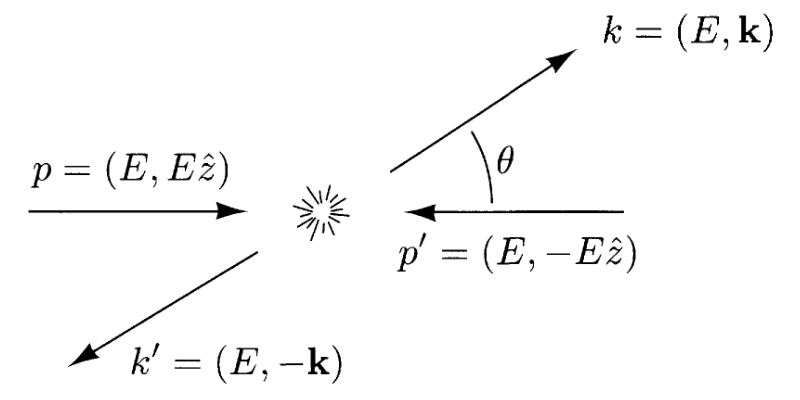
\includegraphics[width = 0.50 \textwidth]{images/com-rf.png}
  \caption{Center-of-mass RF for a $ 2 \rightarrow 2 $ scattering process.}
  \label{com-rf}
\end{figure}

Note that this is the most genera expression for $ 2 \rightarrow 2 $ scattering with $ m_{i_1} = m_{i_2} $ and $ m_{f_1} = m_{f_2} $. In this frame, the Mandelstam variables are:
\begin{equation*}
  s = 4E^2 \equiv E_\text{cm}^2
\end{equation*}
\begin{equation*}
  t = -2 (E^2 - E \abs{\ve{k}} \cos \theta) + m_e^2 + m_\mu^2 \approx -2E (E - \abs{\ve{k}} \cos \theta) + m_\mu^2
\end{equation*}
\begin{equation*}
  u = -2 (E^2 + E \abs{\ve{k}} \cos \theta) + m_e^2 + m_\mu^2 \approx -2E (E - \abs{\ve{k}} \cos \theta) + m_\mu^2
\end{equation*}
Inserting into \eref{eq:mat-el-mand}:
\begin{equation*}
  \begin{split}
    \abs{\mathcal{M}}^2
    & = \frac{2e^4}{16 E^4} \left[ 4E^2 (E - \abs{\ve{k}} \cos \theta)^2 + 4E^2 (E - \abs{\ve{k}} \cos \theta)^2 + 8 m_\mu^2 E^2 \right] \\
    & = \frac{e^4}{2E^2} \left[ (E - \abs{\ve{k}} \cos \theta)^2 + (E - \abs{\ve{k}} \cos \theta)^2 + 2m_\mu^2 \right] \\
    & = e^4 \left[ 1 + \frac{\abs{\ve{k}}^2}{E^2} \cos^2 \theta + \frac{m_\mu^2}{E^2} \right] = \left[ 1 + \frac{m_\mu^2}{E^2} + \left( 1 - \frac{m_\mu^2}{E^2} \right) \cos^2 \theta \right]
  \end{split}
\end{equation*}

\subsubsection{Unpolarized cross-section}

In general, the \bctxt{cross-section} generalizes the geometric section of an object in the context of scattering processes.












\part{Renormalization}
\pagestyle{body}

\chapter{1-Loop Renormalization}
\selectlanguage{english}

As already noted in \secref{sssec:div}, the computation of Next-to-Leading Order (NLO) corrections often produces diverging amplitudes. However, this seems to be a consequence of Heisenberg's principle, implying that a quantum field theory cannot be valid at all energy scales at once.

\section{Renormalization of \texorpdfstring{$ \lambda \phi^4 $}{λφ4}-theory}

\subsection{1-Loop diagrams}
\label{ssec:f4-1-loop}

Consider $ \lambda \phi^4 $-theory and compute the scattering cross-section for $ \phi \phi \rightarrow \phi \phi $ at LO:
\begin{equation*}
  \begin{tikzpicture}[baseline=(r.base)]
    \begin{feynman}[inline=(r.base)]
      \vertex (a1) {};
      \vertex[right=4cm of a1] (a2) {};
      \vertex[below=4em of a1] (b1) {};
      \vertex[below=4em of a2] (b2) {};
      \vertex[below=2em of a1] (c1) {};
      \vertex[right=2cm of c1, dot] (c2) {};

      \vertex[below=2.2em of a1] (r);

      \diagram* {
        (a1) -- [scalar, momentum = \(p_1\)] (c2),
        (b1) -- [scalar, momentum' = \(p_2\)] (c2),
        (c2) -- [scalar, momentum = \(p_3\)] (a2),
        (c2) -- [scalar, momentum' = \(p_4\)] (b2),
      };
    \end{feynman}
  \end{tikzpicture}
  \qquad \Rightarrow \qquad
  \dd \sigma^\text{LO} = \frac{1}{\Phi} \frac{\dd^3p_3}{(2\pi)^3 2E_{p_3}} \frac{\dd^3p_4}{(2\pi)^4 2E_{p_4}} (2\pi)^4 \delta^{(4)}(p_1 + p_2 - p_3 - p_4) \lambda^2
\end{equation*}
In the CM frame:
\begin{equation*}
  p_1 = (E, 0, 0, p)
  \quad
  p_2 = (E, 0, 0, -p)
  \qquad
  p_3 = (E, p \sin \theta, 0, p \cos \theta)
  \quad
  p_4 = (E, -p \sin \theta, 0, - p \cos \theta)
\end{equation*}
\begin{equation*}
  s = 4E^2
  \qquad
  t = -2p^2 (1 + \cos \theta)
  \qquad
  u = -2p^2 (1 - \cos \theta)
\end{equation*}
with flux factor $ \Phi = 8pE $. Then the cross-section becomes:
\begin{equation*}
  \dd \sigma^\text{LO} = \frac{\lambda^2}{8pE} \frac{\dd^3p_3}{(2\pi)^2 (2E_{p_3})^2} \delta(2E - 2\sqrt{p_3^2 + m^2}) = \frac{\lambda^2}{8pE} \frac{p_3 \dd p_3 \dd \Omega_2}{(2\pi)^2 4E_{p_3}} \delta(E_{p_3} - E) = \frac{\lambda^2}{8pE} \frac{p}{16\pi E} \dd \cos \theta
\end{equation*}
Therefore, there's no angular dependence:
\begin{equation}
  \frac{\dd \sigma^\text{LO}}{\dd \cos \theta} = \frac{\lambda^2}{128 \pi} \frac{1}{E^2}
\end{equation}
Now, consider the NLO corrections to this cross-section, i.e. the 1-loop corrections:
\begin{equation*}
  \begin{tikzpicture}[baseline=(r.base)]
    \begin{feynman}[inline=(r.base)]
      \vertex (a1) {};
      \vertex[right=4cm of a1] (a2) {};
      \vertex[below=4em of a1] (b1) {};
      \vertex[below=4em of a2] (b2) {};
      \vertex[below=2em of a1] (c1) {};
      \vertex[right=2cm of c1, blob] (c2) {};

      \vertex[below=2.2em of a1] (r);

      \diagram* {
        (a1) -- [scalar, momentum = \(p_1\)] (c2),
        (b1) -- [scalar, momentum' = \(p_2\)] (c2),
        (c2) -- [scalar, momentum = \(p_3\)] (a2),
        (c2) -- [scalar, momentum' = \(p_4\)] (b2),
      };
    \end{feynman}
  \end{tikzpicture}
  \quad = \quad
  \begin{tikzpicture}[baseline=(r.base)]
    \begin{feynman}[inline=(r.base)]
      \vertex (a1) {};
      \vertex[right=4cm of a1] (a2) {};
      \vertex[below=4em of a1] (b1) {};
      \vertex[below=4em of a2] (b2) {};
      \vertex[below=2em of a1] (c1) {};
      \vertex[right=2cm of c1, dot] (c2) {};

      \vertex[below=2.2em of a1] (r);

      \diagram* {
        (a1) -- [scalar, momentum = \(p_1\)] (c2),
        (b1) -- [scalar, momentum' = \(p_2\)] (c2),
        (c2) -- [scalar, momentum = \(p_3\)] (a2),
        (c2) -- [scalar, momentum' = \(p_4\)] (b2),
      };
    \end{feynman}
  \end{tikzpicture}
  \quad + \smo(\lambda^2) \equiv -i \lambda F(s,t)
\end{equation*}
where $ F(s,t) $ is called \bctxt{form factor}.

\begin{proposition}{Form factor}{}
  In $ \lambda \phi^4 $-theory, the form factor at NLO is:
  \begin{equation}
    F(s,t) = 1 - i\lambda \left( V(s) + V(t) + V(u) \right) + \smo(\lambda^2)
  \end{equation}
  with:
  \begin{equation}
    V(p^2) \defeq \frac{1}{2} \int \frac{\dd^4k}{(2\pi)^4} \frac{i}{k^2 - m^2} \frac{i}{(p + k)^2 - m^2}
    \label{eq:vps-def}
  \end{equation}
\end{proposition}

\begin{proofbox}
  \begin{proof}
    The NLO correction to the scattering amplitude is given by three loop diagrams:
    \begin{equation*}
      \begin{tikzpicture}[baseline = (r.base)]
        \begin{feynman}[inline = (r.base)]
          \vertex (x1) {};
          \vertex[below=3em of x1] (p1) {};
          \vertex[below=3em of p1] (x2) {};

          \vertex[right=3em of p1, dot] (v1) {};
          \vertex[right=5em of v1, dot] (v2) {};

          \vertex[right=3em of v2] (p2) {};
          \vertex[above=3em of p2] (x3) {};
          \vertex[below=3em of p2] (x4) {};

          \vertex[above=0.5em of v1] (r) {};

          \diagram* {
            (x1) -- [scalar, momentum = \(p_1\)] (v1),
            (x2) -- [scalar, momentum' = \(p_2\)] (v1),
            (v2) -- [scalar, momentum = \(p_3\)] (x3),
            (v2) -- [scalar, momentum' = \(p_4\)] (x4),

            (v1) -- [scalar, half left, momentum' = \(p'\)] (v2),
            (v2) -- [scalar, half left, momentum' = \(p\)] (v1),
          };
        \end{feynman}
      \end{tikzpicture}
      \qquad
      \begin{tikzpicture}[baseline = (r.base)]
        \begin{feynman}[inline = (r.base)]
          \vertex (x1) {};
          \vertex[right=4em of x1] (p1) {};
          \vertex[right=4em of p1] (x3) {};

          \vertex[below=2em of p1, dot] (v1) {};
          \vertex[below=5em of v1, dot] (v2) {};

          \vertex[below=9em of x1] (x2) {};
          \vertex[below=9em of x3] (x4) {};

          \vertex[below=2em of v1] (r) {};

          \diagram* {
            (x1) -- [scalar, momentum = \(p_1\)] (v1) -- [scalar, momentum = \(p_3\)] (x3),
            (x2) -- [scalar, momentum' = \(p_2\)] (v2) -- [scalar, momentum' = \(p_4\)] (x4),

            (v1) -- [scalar, half left, momentum = \(p + p_1 - p_3\)] (v2),
            (v2) -- [scalar, half left, momentum = \(p\)] (v1),
          };
        \end{feynman}
      \end{tikzpicture}
      \qquad
      \begin{tikzpicture}[baseline = (r.base)]
        \begin{feynman}[inline = (r.base)]
          \vertex (x1) {};
          \vertex[right=4em of x1] (p1) {};
          \vertex[right=4em of p1] (x3) {};

          \vertex[below=2em of p1, dot] (v1) {};
          \vertex[below=5em of v1, dot] (v2) {};

         \vertex[below=9em of x1] (x2) {};
          \vertex[below=9em of x3] (x4) {};

          \vertex[below=2em of v1] (r) {};

          \diagram* {
            (x1) -- [scalar, momentum = \(p_1\)] (v1) -- [scalar, momentum = \(p_4\)] (x3),
            (x2) -- [scalar, momentum' = \(p_2\)] (v2) -- [scalar, momentum' = \(p_3\)] (x4),

            (v1) -- [scalar, half left, momentum = \(p + p_1 - p_4\)] (v2),
            (v2) -- [scalar, half left, momentum = \(p\)] (v1),
          };
        \end{feynman}
      \end{tikzpicture}
    \end{equation*}
    with $ p' = p_1 + p_2 + p $. These correspond to loop diagrams in the $ s $, $ t $ and $ u $ channels, therefore, recalling \eref{eq:f4-loop-ampl}, the thesis is trivially found.
  \end{proof}
\end{proofbox}

\begin{lemma}[before upper = {\tcbtitle}]{Feynman parameters}{}
  \begin{equation}
    \frac{1}{AB} = \int_0^1 \dd x \frac{1}{\left( x A + (1-x) B \right)^2}  
  \end{equation}
\end{lemma}

This allows to rewrite $ V(p^2) $:
\begin{equation*}
  V(p^2) = - \frac{1}{2} \int \frac{\dd^4k}{(2\pi)^4} \int_0^1 \dd x \left[ k^2 - m^2 + x \left( 2 k \cdot p + p^2 \right) \right]^{-2} \equiv - \frac{1}{2} \int_0^1 \dd x \int \frac{\dd^4\ell}{(2\pi)^4} \frac{1}{\left( \ell^2 - M^2 \right)^2}
\end{equation*}
having defined:
\begin{equation}
  \ell \equiv k + x p
  \qquad \qquad
  M^2 \equiv m^2 - x (1-x) p^2
\end{equation}

\begin{lemma}[before upper = {\tcbtitle}]{}{}
  \begin{equation}
    I_d(n) \equiv \int \frac{\dd^dk}{(2\pi)^d} \frac{1}{(k^2 - M^2 + i\epsilon)^n} = \frac{i (-1)^n}{(4\pi)^{d/2}} \frac{\Gamma(n - \frac{d}{2})}{\Gamma(n)} \left( \frac{1}{M^2} \right)^{n - d/2}
    \label{eq:int-dn}
  \end{equation}
\end{lemma}

\begin{proofbox}
  \begin{proof}
    The poles of the integrand function are $ k_0 = \pm \left[ \sqrt{M^2 + \ve{k}^2} - i\epsilon \right] $, therefore the integration path $ I = \R $ can be rotated counterclockwise by $ \frac{\pi}{2} $ without overlapping with any pole. The resulting Wick rotation $ k_0 \mapsto i k_0 $, i.e. $ k \mapsto k_\text{E} $ implies $ k_E \in \R $, therefore the $ d $-dimensional integral in Minkowskian metric becomes a $ d $-dimensional integral with (negative) Euclidean metric:
    \begin{equation*}
      I_d(n) = i (-1)^n \int \frac{\dd^dk_\text{E}}{(2\pi)^d} \frac{1}{(k_\text{E}^2 + M^2 - i\epsilon)^n} = i (-1)^n \int_{\mathbb{S}^d} \dd \Omega_d \int_{\R^+} \dd k_\text{E} \frac{k_\text{E}^{d-1}}{(k_\text{E}^2 + M^2)^n}
    \end{equation*}
    It can be shown that:
    \begin{equation}
      \int_{\R^+} \dd k_\text{E} \frac{k_\text{E}^{d-1}}{(k_\text{E}^2 + M^2)^n} = \frac{1}{2} \frac{\Gamma(n - \frac{d}{2}) \Gamma(\frac{d}{2})}{\Gamma(n)} \left( \frac{1}{M^2} \right)^{n - \frac{d}{2}}
    \end{equation}
    Inserting \eref{eq:solid-angle} yields the thesis.
  \end{proof}
\end{proofbox}

\eref{eq:int-dn} diverges for $ (d,n) = (4,2) $, as $ \Gamma(z) = \frac{1}{z} - \gamma_\text{E} + o(z) $, therefore a cutoff needs to be introduced to regularize the integral:
\begin{equation*}
  \begin{split}
    V(p^2)
    & = \lim_{\Lambda \rightarrow \infty} \frac{-i}{2} \int_0^1 \dd x \int_0^\Lambda \frac{\dd k_\text{E}}{8\pi^2} \frac{k_\text{E}^3}{(k_\text{E}^2 + M^2)^2} = \lim_{\Lambda \rightarrow \infty} \frac{-i}{2} \int_0^1 \dd x \int_{M^2}^{\Lambda^2 + M^2} \frac{\dd \rho}{16\pi^2} \frac{\rho - M^2}{\rho^2} \\
    & = \lim_{\Lambda \rightarrow \infty} \frac{-i}{32 \pi^2} \int_0^1 \dd x \left[ \log \left( 1 + \frac{\Lambda^2}{M^2} \right) - \frac{\Lambda^2}{\Lambda^2 + M^2} \right] \\
    & = \lim_{\Lambda \rightarrow \infty} \frac{-i}{32\pi^2} \int_0^1 \dd x \left[ \log \frac{\Lambda^2}{M^2} - 1 + \smo  \left( \frac{M^2}{\Lambda^2} \right) \right]
  \end{split}
\end{equation*}
The form factor can then be rewritten as:
\begin{equation}
  F(s,t) = 1 + \frac{\lambda}{32\pi^2} \left[ 3 + \lim_{\Lambda \rightarrow \infty} \int_0^1 \dd x \left( \log \frac{M^2(s)}{\Lambda^2} + \log \frac{M^2(t)}{\Lambda^2} + \log \frac{M^2(u)}{\Lambda^2} \right) \right] + \smo(\lambda^2)
  \label{eq:form-factor}
\end{equation}
Now, define the threshold values $ s_0 \equiv 4m^2 $, $ t_0 = u_0 \equiv 0 $. The \bctxt{physical coupling constant} $ \lambda_\text{phys} $ is defined as:
\begin{equation}
  \frac{\dd \sigma}{\dd \cos \theta}\bigg\vert_{s_0 , t_0} = \frac{\lambda_\text{phys}^2}{128\pi m^2}
\end{equation}
which is linked to the \bctxt{bare coupling constant} $ \lambda_\text{bare} \equiv \lambda $ by:
\begin{equation}
  \lambda_\text{bare} F(s_0,t_0) = \lambda_\text{phys}
  \label{eq:bare-phys-def}
\end{equation}

\begin{proposition}{Bare and physical coupling}{bare-phys-coupl}
  The NLO form factor can be expressed as:
  \begin{equation}
    \lambda F(s,t) = \lambda_\text{phys} \left[ 1 - \frac{\lambda_\text{phys}}{32\pi^2} \int_0^1 \dd x \left( \log \frac{M^2(s)}{M^2(s_0)} + \log \frac{M^2(t)}{M^2(t_0)} + \log \frac{M^2(u)}{M^2(u_0)} \right) \right] + \smo(\lambda_\text{phys}^3)
    \label{eq:l-f-cutoff}
  \end{equation}
\end{proposition}

\begin{proofbox}
  \begin{proof}
    By \eref{eq:bare-phys-def}:
    \begin{equation*}
      \lambda_\text{phys} = \lambda (1 - c_0 \lambda) + \smo(\lambda^3)
      \qquad \Leftrightarrow \qquad
      \lambda = \lambda_\text{phys} (1 + c_0 \lambda_\text{phys}) + \smo(\lambda_\text{phys}^3)
    \end{equation*}
    Therefore:
    \begin{equation*}
      \lambda (1 - c \lambda) = \lambda_\text{phys} (1 + c_0 \lambda_\text{phys}) (1 - c \lambda_\text{phys}) + \smo(\lambda_\text{phys}^3) = \lambda_\text{phys} (1 - (c - c_0) \lambda_\text{phys}) + \smo(\lambda_\text{phys}^3)
    \end{equation*}
    Inserting \eref{eq:form-factor} yields the thesis.
  \end{proof}
\end{proofbox}

Expressing $ \lambda_\text{bare} $ as a function of $ \lambda_\text{phys} $ eliminates the divergence regularized by the cutoff, which is absorbed into $ \lambda_\text{phys} $, which is the observable coupling constant. Note that the choice of $ s_0 $ and $ t_0 $ to define $ \lambda_\text{phys} $ is purely conventional: a more useful choice is imposing:
\begin{equation}
  M^2(s_0) = M^2(t_0) = M^2(u_0) = \mu^2
\end{equation}
It is important to stress the difference between $ \Lambda $ and $ \mu $: $ \Lambda $ is a \bctxt{regularization scale}, introduced to regularize diverging loop integrals, while $ \mu $ is a \bctxt{renormalization point}, introduced to eliminate the $ \Lambda $-depedence\footnotemark. Both parameters are arbitrary, hence physical observables cannot depend on any of them: this means that the explicit $ \mu $-dependence of $ F(s,t) $ must cancel the implicit $ \mu $-dependence of $ \lambda $, so that $ \lambda_\text{phys} $. \\
The infinities which cancel expressing $ F(s,t) $ in terms of $ \lambda_\text{phys} $ are explicit when expressing $ \lambda_\text{bare} = \lambda_\text{bare}(\lambda_\text{phys}) $. In fact:
\begin{equation*}
  \lambda_\text{phys} = \lambda_\text{bare} \left[ 1 + \frac{3\lambda_\text{bare}}{32\pi^2} \left( 1 + \log \frac{\mu^2}{\Lambda^2} \right) \right] + \smo(\lambda_\text{bare}^3)
\end{equation*}
Thus, choosing $ \mu^2 \propto \Lambda^2 $, it is possible to express $ \lambda_\text{phys} $ as a limit of $ \lambda_\text{bare} $, and eventually $ \lambda_\text{phys} = \lambda_\text{bare} $: the bare coupling constant is the physical coupling at the scale $ \Lambda \rightarrow \infty $ (infinitely-small distances), i.e. including the fluctuations at all scales. Due to Heisenberg's principle, then, $ \lambda_\text{bare} $ is expected to diverge: excitations of the fields in momentum space are defined as normal coordinates of the system in position space, i.e. $ p \sim \pa_x \phi \sim \frac{1}{\Delta x} $, which diverges as $ \Delta x \rightarrow 0 $ (as $ \Lambda \rightarrow \infty $).

\footnotetext{The regularization scale $ \Lambda $ is an unphysical artifact introduce to isolate UV divergences, it depends on the specific regularization scheme adopted (UV cut-off, dimensional regolarization, etc.) and it disappears in renormalized results, while the renormalization point $ \mu $ is the physical reference scale which defines renormalized physical parameters.}

\subsection{Renormalized perturbation theory}

The process of renormalization, which allows to obtain finite results from diverging amplitudes, can be implemented in various ways. That of introducing a UV cut-off $ \Lambda $, expressing the bare observables in terms of the physical observables at some scale $ \mu $ and then setting $ \Lambda \rightarrow \infty $ is rather inefficient at higher orders in perturbation theory: thus, a more efficient renormalization scheme must be adopted. \\
First of all, substitute the UV cut-off with a \bctxt{dimensional regularization scheme} ('t Hooft--Veltman scheme): this scheme consists in turning diverging loop integrals into meromorphic\footnotemark functions of $ d \in \C $, which is an analytic continuation of the number of spacetime dimensions. In particular:
\begin{equation}
  d = 4 - 2 \epsilon
\end{equation}
with $ \epsilon \in \C : \Re{\epsilon} < 0 $. By analytic continuation of the Lagrangian of the theory, the dimensionality of the various objects changes.

\footnotetext{Given an open set $ D \subset \C $, then $ f : D \rightarrow \C $ is \textit{meromorphic} if it is holomorphic on $ D - P $, where $ P \subset D $ is a set of isolated points called \textit{poles}. Recall that a function $ f : D \rightarrow \C $ is \textit{holomorphic} on $ D $ if it is complex differentiable at every point in $ D $.}

\begin{proposition}{Dimensional analysis}{}
  In $ d = 4 $:
  \begin{equation}
    [\phi] = [M]
    \qquad \qquad
    [\lambda] = 1
  \end{equation}
\end{proposition}

\begin{proofbox}
  \begin{proof}
    In natural units $ \hbar = c = 1 $, each physical quantity has the dimension of a power of mass, as:
    \begin{equation*}
      [\hbar] = [E] [T] = [M] [T] \equiv 1
      \qquad \qquad
      [c] = [L] [T]^{-1} \equiv 1
    \end{equation*}
    where $ E = m $ ($ c^2 = 1 $) was used. Therefore, $ [L] = [T] = [M]^{-1} $. In this system, the action must be a dimensionless quantity:
    \begin{equation*}
      \act = \int \dd^4x \,\lag
      \qquad \Rightarrow \qquad
      1 = [L]^4 [\lag] = [M]^{-4} [\lag]
      \qquad \Rightarrow \qquad
      [\lag] = [M]^4
    \end{equation*}
    As $ [\pa_\mu] = [L]^{-1} = [M] $, then, it is clear that $ [\phi] = [M] $ and, being $ \lag_\text{int} = - \frac{\lambda}{4!} \phi^4 $, $ [\lambda] = 1 $.
  \end{proof}
\end{proofbox}

\begin{proposition}{Dimensionality in 't Hooft--Veltman scheme}{}
  In $ d = 4 - 2\epsilon $:
  \begin{equation}
    [\phi] = [M]^{1 - \epsilon}
    \qquad \qquad
    [\lambda] = [M]^{2\epsilon}
  \end{equation}
\end{proposition}

\begin{proofbox}
  \begin{proof}
    In the dimensional regularization scheme the differential becomes $ \dd^4x \mapsto \dd^dx $, therefore the Lagrangian must have:
    \begin{equation*}
      [\lag] = [M]^d = [M]^{4 - 2\epsilon}
    \end{equation*}
    $ [\pa_\mu] = [M] $ remains unchanged, therefore $ [\phi] = [M]^{1 - \epsilon} $ and, as a consequence, $ [\lambda] = [M]^{2\epsilon} $.
  \end{proof}
\end{proofbox}

To explicit the dimensionality of the (bare) coupling constant, a regularization scale $ \mu_\text{reg} $ is introduced, so that:
\begin{equation}
  \lambda = \mu_\text{reg}^{2\epsilon} \lambda_\text{bare}
\end{equation}

\begin{proposition}{}{}
  In $ d = 4 - 2\epsilon $:
  \begin{equation}
    -i \lambda V(p^2) = - \frac{\lambda_\text{bare}}{32\pi^2} \int_0^1 \dd x \left[ \frac{1}{\epsilon} - \gamma_\text{E} + \ln 4\pi - \log \frac{M^2}{\mu_\text{reg}^2} + \smo(\epsilon) \right]
  \end{equation}
  where $ \gamma_\text{E} \simeq 0.5772 $ is the Euler--Mascheroni constant.
\end{proposition}

\begin{proofbox}
  \begin{proof}
    From \eref{eq:vps-def} and using \eref{eq:int-dn}:
    \begin{equation*}
      \begin{split}
        -i \lambda V(p^2)
        & = \frac{i \lambda}{2} \int_0^1 \dd x \int \frac{\dd^d\ell}{(2\pi)^d} \frac{1}{(\ell^2 - M^2)^2} = \frac{i \lambda_\text{bare}}{2} \mu_\text{reg}^{2\epsilon} \int_0^1 \dd x \frac{i}{(4\pi)^{2 - \epsilon}} \frac{\Gamma(\epsilon)}{2} (M^2)^{-\epsilon} \\
        & = - \frac{\lambda_\text{bare}}{32\pi^2} \int_0^1 \dd x \, (4\pi)^\epsilon \Gamma(\epsilon) \left( \frac{M^2}{\mu_\text{reg}^2} \right)^{-\epsilon}
      \end{split}
    \end{equation*}
    Now, the Laurent series in $ \epsilon $ for this expression is:
    \begin{equation*}
      \begin{split}
        -i \lambda V(p^2)
        &= - \frac{\lambda_\text{bare}}{32\pi^2} \int_0^1 \dd x \left( 1 + \epsilon \log 4\pi + \smo(\epsilon) \right) \left( \frac{1}{\epsilon} - \gamma_\text{E} + \smo(\epsilon) \right) \left( 1 - \epsilon \log \frac{M^2}{\mu_\text{reg}^2} + \smo(\epsilon) \right) \\
        & = - \frac{\lambda_\text{bare}}{32\pi^2} \int_0^1 \dd x \left[ \frac{1}{\epsilon} - \gamma_\text{E} + \log 4\pi - \log \frac{M^2}{\mu_\text{reg}^2} + \smo(\epsilon) \right]
      \end{split}
    \end{equation*}
    which is the thesis.
  \end{proof}
\end{proofbox}

The dimensionally-regularized form factor, then, takes the form:
\begin{equation*}
  F(s,t) = 1 - \frac{\lambda_\text{bare}}{32\pi^2} \left[ 3 \left( \frac{1}{\epsilon} - \gamma_\text{E} + \log 4\pi \right) - \int_0^1 \dd x \left( \log \frac{M^2(s)}{\mu_\text{reg}^2} + \log \frac{M^2(t)}{\mu_\text{reg}^2} + \log \frac{M^2(u)}{\mu_\text{reg}^2} \right) \right] + \smo(\epsilon)
\end{equation*}
It would then be possible to proceed with the renormalization of the coupling constant specifying a cinematic $ (s_0,t_0) $ and setting $ \lambda_\text{phys} = \lambda_\text{bare} F(s_0,t_0) $. However, given the arbitrariness of the renormalization point $ \mu_\text{ren} $, it is algebrically convenient to choose an unphysical cinematic which simplifies the expression of $ \lambda_\text{phys} $.

\begin{definition}{Minimal subtraction scheme}{}
  The \bcdef{minimal subtraction scheme} (MS) is a renormalization scheme with renormalization point such that:
  \begin{equation}
    \lambda_\text{MS} = \lambda_\text{bare} \left[ 1 - \frac{3\lambda_\text{bare}}{32\pi^2} \frac{1}{\epsilon} \right] + \smo(\lambda_\text{bare}^3)
  \end{equation}
\end{definition}

When working with dimensional regularization, it is more useful to adopt the \bctxt{modified MS scheme} ($ \msb $), which includes the universal constant $ -\gamma_\text{E} + \log 4\pi $ in the expression for the physical coupling constant:
\begin{equation}
  \lambda_{\msb} = \lambda_\text{bare} \left[ 1 - \frac{3\lambda_\text{bare}}{32\pi^2} \left( \frac{1}{\epsilon} - \gamma_\text{E} + \log 4\pi \right) \right] + \smo(\lambda_\text{bare}^3)
  \label{eq:l-msb}
\end{equation}

\begin{theorem}{Scales in the $ \msb $ scheme}{}
  In the $ \msb $ scheme:
  \begin{equation}
    \mu_\text{reg} = \mu_\text{ren}
  \end{equation}
\end{theorem}

\begin{proofbox}
  \begin{proof}
    As of \eref{eq:l-msb}, using the same reasoning as in the proof of \pref{prop:bare-phys-coupl}:
    \begin{equation}
      \lambda_\text{bare} = \lambda_{\msb} \left[ 1 + \frac{3\lambda_{\msb}}{32\pi^2} \left( \frac{1}{\epsilon} - \gamma_\text{E} + \log 4\pi \right) \right] + \smo(\lambda_{\msb}^3)
    \end{equation}
    Moreover:
    \begin{equation*}
      \begin{split}
        \lambda_\text{bare} F(s,t)
        & = \lambda_\text{bare} \left[ 1 - \frac{3\lambda_\text{bare}}{32\pi^2} \left( \frac{1}{\epsilon} - \gamma_\text{E} + \log 4\pi \right) \right] \\
        & \qquad \qquad \qquad \qquad  + \frac{\lambda_\text{bare}^2}{32\pi^2} \int_0^1 \dd x \left( \log \frac{M^2(s)}{\mu_\text{reg}^2} + \log \frac{M^2(t)}{\mu_\text{reg}^2} + \log \frac{M^2(u)}{\mu_\text{reg}^2} \right) + \smo(\lambda_\text{bare}^3) \\
      \end{split}
    \end{equation*}
    Then, noting that $ \lambda_\text{bare}^2 = \lambda_{\msb}^2 + \smo(\lambda_{\msb}^3) $:
    \begin{equation*}
      \lambda_\text{bare} F(s,t) = \lambda_{\msb} \left[ 1 + \frac{\lambda_{\msb}}{32\pi^2} \int_0^1 \dd x \left( \log \frac{M^2(s)}{\mu_\text{reg}^2} + \log \frac{M^2(t)}{\mu_\text{reg}^2} + \log \frac{M^2(u)}{\mu_\text{reg}^2} \right) \right] + \smo(\lambda_{\msb}^3)
    \end{equation*}
    Comparing this expression to \eref{eq:l-f-cutoff}, it is clear that $ \mu_\text{reg} $ is also the renormalization point of the scheme.
  \end{proof}
\end{proofbox}

Hence, in the $ \msb $ scheme $ \mu_\text{reg} = \mu_\text{ren} \equiv \mu $.

\subsubsection{Lagrangian counterterms}
\label{sssec:lag-count}

Define $ Z_\lambda : \lambda_\text{bare} = Z_\lambda \lambda_{\msb} \equiv \lambda_{\msb} + \delta_\lambda $, so that:
\begin{equation*}
  Z_\lambda = 1 + \frac{3\lambda_{\msb}}{32\pi^2} \left( \frac{1}{\epsilon} - \gamma_\text{E} + \log 4\pi \right) + \smo(\lambda_{\msb}^2)
  \qquad
  \delta_\lambda = 1 + \frac{3\lambda_{\msb}}{32\pi^2} \left( \frac{1}{\epsilon} - \gamma_\text{E} + \log 4\pi \right) + \smo(\lambda_{\msb}^3)
\end{equation*}
Inserting into the Lagrangian:
\begin{equation*}
  \begin{split}
    \lag
    & = \frac{1}{2} \left( \pa_\mu \phi \pa^\mu \phi - m^2 \phi^2 \right) - \frac{\lambda}{4!} \phi^4 \\
    & = \frac{1}{2} \left( \pa_\mu \phi \pa^\mu \phi - m^2 \phi^2 \right) - \frac{\lambda_{\msb}}{4!} \phi^4 - \frac{\delta_\lambda}{4!} \phi^4 + \smo(\lambda_{\msb}^3)
  \end{split}
\end{equation*}
It is then clear that renormalizing the coupling constant is equivalent to adding a counterterm to the Lagrangian, which contains the original divergence. This counterterm induces a new interaction vertex:
\begin{equation}
  \begin{tikzpicture}[baseline=(r.base)]
    \begin{feynman}[inline=(r.base)]
      \vertex (a1) {};
      \vertex[right=4cm of a1] (a2) {};
      \vertex[below=4em of a1] (b1) {};
      \vertex[below=4em of a2] (b2) {};
      \vertex[below=2em of a1] (c1) {};
      \vertex[right=2cm of c1, crossed dot] (c2) {};

      \vertex[below=2.2em of a1] (r);

      \diagram* {
        (a1) -- [scalar] (c2),
        (b1) -- [scalar] (c2),
        (c2) -- [scalar] (a2),
        (c2) -- [scalar] (b2),
      };
    \end{feynman}
  \end{tikzpicture}
  \quad = \quad -i \delta_\lambda
  \label{eq:counterterm}
\end{equation}
This process is general: divergences are cured order by order in perturbation theory by adding each time new counterterms to the Lagrangian: hence the name of renormalized perturbation theory\footnote{The name may be confusing, as the counterterms still contain divergences.}. At each order, each new counterterms are fixed by an appropriate physical condition.

\subsection{Renormalizability}

The problem of renormalization has been reduced to that of classifying all possible counterterms to the Lagrangian, where each counterterm arises from the normalization of a different class of diverging Feynman diagrams.

\begin{definition}{Superficial degree of divergence}{}
  Given a scalar field theory in $ d $ dimensions, the \bcdef{superficial degree of divergence} of a Feynman diagram with $ L $ loops and $ P_\text{s} $ scalar propagators is:
  \begin{equation}
    D \defeq d L - 2 P_\text{s}
    \label{eq:sup-deg-div-def}
  \end{equation}
\end{definition}

The superficial degree of divergence gives an idea of how badly the considered diagram diverges: indeed, each loop corresponds to an integration with measure $ \dd^dk $, which has dimension $ [M]^d $, and each propagator corresponds to a factor of $ \tilde{D}_\text{F}(p) \sim (p^2 - m^2)^{-1} $, which has dimension $ [M]^{-2} $, so $ D $ is the net power of momentum present in the amplitude:
\begin{equation*}
  \mat \sim \int \frac{\dd k}{k^{1-D}}
\end{equation*}
Introducing a UV cut-off $ \Lambda $, the divergence will be different for different values of $ D $:
\begin{itemize}
  \item $ D > 0 $: $ \mat \sim \Lambda^D $, hence the diagram has a UV divergence which must be renormalized;
  \item $ D = 0 $: $ \mat \sim \log \Lambda $, hence the diagram has a logarithmic UV divergence;
  \item $ D < 0 $: $ \mat \sim \Lambda^{-\abs{D}} $, hence the diagram is UV finite.
\end{itemize}
This, however, is a naive analysis: in fact, the diagram may have diverging sub-diagrams which make the actual degree of divergence worse, or it may have symmetries which make divergences partially cancel, leaving a better degree of divergence. As an example, a trivial diagram with no loops and no propagators has $ D = 0 $, but it is not a diverging diagram. \\
The problem of diverging sub-diagrams requires a more careful analysis. Consider the following diagram in $ 4 $-dimensional $ \lambda \phi^4 $-theory:
\begin{equation*}
  \begin{tikzpicture}[baseline = (r.base)]
    \begin{feynman}[inline = (r.base)]
      \vertex (a1) {};
      \vertex[right=1.3cm of a1] (a2) {};
      \vertex[right=1.3cm of a2] (a3) {};

      \vertex[above=1.3cm of a2, dot] (b1) {};
      \vertex[above=2.6cm of b1, dot] (b2) {};

      \vertex[above=1.3cm of b2] (c2) {};
      \vertex[left=1.3cm of c2, dot] (c1) {};
      \vertex[above=1.3cm of c1] (c4) {};
      \vertex[right=1.3cm of c2, dot] (c3) {};
      \vertex[above=1.3cm of c3] (c5) {};

      \vertex[left=1.3cm of c1] (d1) {};
      \vertex[above=1.3cm of d1] (d2) {};
      \vertex[right=1.3cm of c3] (d3) {};
      \vertex[above=1.3cm of d3] (d4) {};

      \vertex[below=0.5cm of b2] (r) {};

      \diagram* {
        (a1) -- [scalar] (b1) -- [scalar] (a3),
        (b1) -- [scalar, half left] (b2) -- [scalar, half left] (b1),
        (b2) -- [scalar] (c1) -- [scalar] (d2),
        (b2) -- [scalar] (c3) -- [scalar] (d4),
        (c4) -- [scalar] (c1) -- [scalar] (c3) -- [scalar] (c5),
      };
    \end{feynman}
  \end{tikzpicture}
  \qquad \qquad
  D = 4 \cdot 2 - 2 \cdot 5 = -2
\end{equation*}
Although $ D < 0 $, the loop integral diverges: however, in renormalized perturbation theory this divergence is cured by the counterterm \eref{eq:counterterm} This is a general property: apart from superficially divergent diagrams, the only other divergences arise from diverging sub-diagrams of superficially finite diagrams, but these divergences are cured by the counterterms already added to the Lagrangian. Hence, the renormalization procedure correctly cures all UV divergences.

\begin{theorem}{Bogolyubov--Parasyuk theorem}{}
  For any renormalized quantum field theory, the perturbative expansion of matrix elements of the $ S $-matrix is UV-finite.
\end{theorem}

\begin{proofbox}
  \begin{proof}
    The proof is found in \cite{bog-par, azp}.
  \end{proof}
\end{proofbox}

\subsubsection{\texorpdfstring{$ \lambda \phi^n $}{λφn}-theory}

\begin{lemma}{Loop number}{}
  Given a diagram with $ P $ propagators and $ V $ vertices, then:
  \begin{equation}
    L = P - V + 1
    \label{eq:loop-num}
  \end{equation}
\end{lemma}

\begin{proofbox}
  \begin{proof}
    Each loop is associated to an unconstrained momentum: each propagator corresponds to a momentum, while each vertex to a $ \delta $ which constrains the momenta of the diagram, but there's also an overall momentum-conserving $ \delta $ which makes one of the vertex-associated $ \delta $ redundant, hence $ L = P - (V - 1) $, which is the thesis.
  \end{proof}
\end{proofbox}

This result is valid in general for any field theory, and $ P $ represents the total number of propagators (even of different kinds). \\
Considering the specific case of $ \lambda \phi^n $-theory, instead, there's another relation which can simplify the computation of the superficial degrees of freedom: as each vertex has $ n $ scalar lines, then:
\begin{equation}
  n V = 2 P_\text{s} + N_\text{s}
  \label{eq:fn-v}
\end{equation}
where $ N_\text{s} $ is the number of external scalar lines. This expression takes into account the fact that each propagator links two vertices.

\begin{theorem}{Superficial degree of divergence}{lfn-sup-deg-div}
  In $ \lambda \phi^n $-theory in $ d $ dimensions, the \bcth{superficial degree of divergence} is:
    \begin{equation}
      D = d + \left( n \frac{d - 2}{2} - d \right) V - \frac{d - 2}{2} N
      \label{eq:lfn-sup-deg-div}
    \end{equation}
\end{theorem}

\begin{proofbox}
  \begin{proof}
    By \eref{eq:fn-v} $ P = \frac{1}{2} (n V - N) $, thus by \eref{eq:loop-num}:
    \begin{equation*}
      L = \left( \frac{n}{2} - 1 \right) V - \frac{N}{2} + 1
    \end{equation*}
    Recalling \eref{eq:sup-deg-div-def}:
    \begin{equation*}
      D = d \left[ \left( \frac{n}{2} - 1 \right) V - \frac{N}{2} + 1 \right] - n V + N = d + \left( n \frac{d - 2}{2} - d \right) V - \frac{d - 2}{2} N
    \end{equation*}
    which is the thesis.
  \end{proof}
\end{proofbox}

\begin{example}{$ \lambda \phi^4 $-theory}{p4-th}
  The case of $ \lambda \phi^4 $-theory in $ 4 $ dimensions is a particularly simple one, as:
  \begin{equation}
    D = 4 - N
  \end{equation}
  Hence, the only classes of diverging diagrams are vacuum-to-vacuum diagrams, which diverge as $ \sim \Lambda^4 $, the $ 1 \rightarrow 1 $ diagrams (i.e. the $ 2 $-point Green function of the theory and all its possible loop corrections), which diverges as $ \sim \Lambda^2 $, and the $ 2 \rightarrow 2 $ scattering, which diverges as $ \sim \log \Lambda $ (agreeing with \eref{eq:form-factor}). In this case there is only a finite number of classes of diverging diagrams.
\end{example}

\tref{th:lfn-sup-deg-div} can be derived also with dimensional analysis alone. In $ d $-dimensional $ \lambda \phi^n $-theory, it is trivial to show that:
\begin{equation*}
  [\phi] = [M]^{\frac{d - 2}{2}}
  \qquad \qquad
  [\lambda] = [M]^{d - n \frac{d - 2}{2}}
\end{equation*}
The dimensionality of $ \lambda $ is the dimensionality of a diagram with a single vertex, i.e. with $ N = n $ amputated legs, and, as diagrams with the same $ N $ have the same dimensionality, of any diagram with $ N = n $: generalizing, the dimensionality of a diagram with $ N $ amputated legs should be $ d - N \frac{d - 2}{2} $. On the other hand, if the diagram has $ V $ vertices, by definition it should have dimension $ [d]^V [M]^D $, thus:
\begin{equation*}
  \left( d - n \frac{d - 2}{2} \right) V + D = d - N \frac{d - 2}{2}
\end{equation*}
which is exactly \eref{eq:lfn-sup-deg-div}. It is then clear that $ D $ decreases as $ V $ increases (i.e. going to higher orders in perturbation theory) if and only if the coupling constant has positive mass dimension, leaving with only three possible classes theories:
\begin{itemize}
  \item super-renormalizable theories: the coupling constant has strictly negative mass dimension, hence there is only a finite number of diverging diagrams.
  \item renormalizable theories: the coupling constant is dimensionless, hence there is only a finite number of classes of diverging diagrams (although their absolute number may be infinite);
  \item non-renormalizable theories: the coupling constant has strictly negative mass dimension, hence there is an infinite number of diverging classes of diagrams.
\end{itemize}
Note that this are general properties, not restricted to real scalar field theories.

\begin{example}{$ d = 4 $ theories}{}
  Consider $ \lambda \phi^n $-theory in $ d = 4 $ dimensions. The coupling constant in $ \lag_\text{int} = - \frac{1}{n!} \lambda \phi^n $ has dimension $ 4 - n $, hence:
  \begin{itemize}
    \item $ \lambda \phi^3 $-theory is super-renormalizable: $ D = 4 - V - N $, thus the only diverging diagrams are the $ 2 $-point Green function (loop corrections have $ D < 0 $) and the single interaction vertex, while all other diagrams have a finite amplitude;
    \item $ \lambda \phi^4 $-theory is renormalizable: $ D = 4 - N $, so the finitely-many classes of diverging diagrams are those listed in \exref{ex:p4-th};
    \item $ \lambda \phi^n $-theory with $ n \ge 5 $ is non-renormalizable: for example, in $ \lambda \phi^5 $-theory $ D = 4 + V - N $, hence increasing the number of vertices increases the superficial degree of divergence, i.e. $ \forall N \in \N_{\ge 2} \, \exists V \in \N : D > 0 $.
  \end{itemize}
\end{example}

It si then clear what is the conceptual distinction between renormalizable and non-renormalizable theories: renormalizable theories can be renormalizable with a finite set of counterterms, which can be fixed with a finite number of physical conditions (i.e. comparison with experiments), while non-renormalizable theories require an infinite set of counterterms, hence having no predictive power (as infinite parameters must be fixed by comparison with experiments). \\
Although at first glance non-renormalizability may seem problematic, in reality it is not. Consider a non-renormalizable theory with coupling constant $ g \propto M^{-k} $, with $ k \in \R^+ $ and some mass scale $ M $, and assume that the theory has already been renormalized up to $ (N - 1) $-point amplitudes, with $ N \in \N_{\ge 2} $: then, an $ N $-point amplitude at typical energy scale $ E $ can be expressed as:
\begin{equation*}
  \mathcal{A}_N(E) = \mathcal{A}^{(0)}_N(E) \left[ 1 + c_1 \frac{E^k}{M^k} + c_2 \frac{E^{2k}}{M^{2k}} + \dots + c_n \frac{E^{nk}}{M^{nk}} \right]
\end{equation*}
where $ c_1, \dots, c_{n-1} $ are finite constant already fixed by physical conditions. As $ c_n $ should be fixed too by a new physical condition, the theory would not be predictive even at order $ n $: however, at low energy $ E \ll M $, this lack of predictivity due to $ c_n $ is negligible, as the quantity $ (E/M)^{nk} $ can be assumed to be below the sensitivity of the experimental apparatus taken into consideration. Therefore, it is clear that non-renormalizable theories are acceptable low-energy theories: they gain predictive power by limiting the set of counterterms to be fixed to those necessary at the desired energy scale, as the ignorance about higher-order divergences is beyond the required accuracy. At $ E \sim M $ the above series expansion diverges, signaling a lack of meaning of the theory: non-renormalizable theories have a built-in scale which provides their limit of validity, while renormalizable theories are in principle valid at all energy scales.

\subsubsection{\texorpdfstring{$ \lambda \phi^4 $}{λφ4}-theory}

Consider $ \lambda \phi^4 $-theory in $ d = 4 $ dimensions:
\begin{equation}
  \lag = \frac{1}{2} \pa_\mu \phi \pa^\mu \phi - \frac{1}{2} m_0^2 \phi^2 - \frac{\lambda_0}{4!} \phi^4
\end{equation}
where $ m_0 , \lambda_0 $ are the bare mass and coupling constant. By \eref{eq:lfn-sup-deg-div}, the superficial degree of divergence of a diagram depends only on the number of external legs, as $ D = 4 - N $; moreover, as the theory is symmetric under $ \phi \rightarrow -\phi $, alla amplitudes with an odd number of external legs vanish. The only classes of divergent diagrams then are:
\begin{equation*}
  \begin{tikzpicture}[baseline=(r.base)]
    \begin{feynman}[inline=(r.base)]
      \vertex (a1) {};
      \vertex[right=4cm of a1] (a2) {};
      \vertex[below=4em of a1] (b1) {};
      \vertex[below=4em of a2] (b2) {};
      \vertex[below=2em of a1] (c1) {};
      \vertex[right=2cm of c1, blob] (c2) {};

      \vertex[below=2.2em of a1] (r);
    \end{feynman}
  \end{tikzpicture}
  \qquad
  \begin{tikzpicture}[baseline=(r.base)]
    \begin{feynman}[inline=(r.base)]
      \vertex (a1) {};
      \vertex[right=4cm of a1] (a2) {};
      \vertex[below=4em of a1] (b1) {};
      \vertex[below=4em of a2] (b2) {};
      \vertex[below=2em of a1] (c1) {};
      \vertex[right=2cm of c1, blob] (c2) {};

      \vertex[left = 2cm of c2] (d1) {};
      \vertex[right = 2cm of c2] (d2) {};

      \vertex[below=2.2em of a1] (r);

      \diagram* {
        (d1) -- [scalar] (c2),
        (c2) -- [scalar] (d2),
      };
    \end{feynman}
  \end{tikzpicture}
  \qquad
  \begin{tikzpicture}[baseline=(r.base)]
    \begin{feynman}[inline=(r.base)]
      \vertex (a1) {};
      \vertex[right=4cm of a1] (a2) {};
      \vertex[below=4em of a1] (b1) {};
      \vertex[below=4em of a2] (b2) {};
      \vertex[below=2em of a1] (c1) {};
      \vertex[right=2cm of c1, blob] (c2) {};

      \vertex[below=2.2em of a1] (r);

      \diagram* {
        (a1) -- [scalar] (c2),
        (b1) -- [scalar] (c2),
        (c2) -- [scalar] (a2),
        (c2) -- [scalar] (b2),
      };
    \end{feynman}
  \end{tikzpicture}
\end{equation*}
The first class is that of vacuum-to-vacuum diagrams, which are unobservable vacuum energy shifts as they are all accounted for in the definition of correlation functions (see \secref{sssec:lamb-4}).
The second class of diagrams are the loop corrections to the $ 2 $-point Green function and, having $ D = 2 $, has the general diverging structure $ \sim c_1 \Lambda^2 + c_2 p^2 \log \Lambda $, where $ p $ is the initial-state four-momentum.
The third class of diagrams are the loop corrections to the $ 2 \rightarrow 2 $ scattering amplitude, with $ D = 0 $ and diverging structure $ \sim c_3 \log \Lambda $ (agreeing with \secref{ssec:f4-1-loop}).
Ignoring the vacuum-to-vacuum diagrams, there are three infinite constants that need to be absorved into three unobservable parameters of the theory: the bare mass, the bare coupling constant and the field-strength.

\paragraph{Correlation functions}

To express the identity operator on the Fock space $ \fock $ of the theory, it is necessary to choose a complete basis of $ \fock $. Consider an eigenstate of the Hamiltonian $ H \ket{\lambda_0} = m_0 \ket{\lambda_0} $ such that $ \ve{P} \ket{\lambda_0} = \ve{0} $ (i.e. $ m_0^2 = E_0^2 $): as per Lorentz invariance, all possible boosts of $ \ket{\lambda_0} $ are still eigenstates of $ H $, and they have all the possible three-momenta. Conversely , any eigenstate of $ H $ with definite three-momentum can be expressed as the boost of some zero-momentum eigenstate $ \ket{\lambda_0} $. Denoting with $ \ket{\lambda_\ve{p}} $ the eigenstate of $ H $ with three-momentum $ \ve{p} $ obtained as a boost of $ \ket{\lambda_0} $ and defining $ E_\ve{p}(\lambda) \equiv \sqrt{\ve{p}^2 + m_\lambda^2} $, where $ m_\lambda : H \ket{\lambda_0} = m_\lambda \ket{\lambda} $, then the completeness relation on $ \fock $ can be written as\footnotemark:
\begin{equation}
  \id_\fock = \ket{0}\bra{0} + \sum_\lambda \int \frac{\dd^3p}{(2\pi)^3} \frac{1}{2E_\ve{p}(\lambda)} \ket{\lambda_\ve{p}}\bra{\lambda_\ve{p}}
\end{equation}
where $ \ket{0} $ is the vacuum state of $ \fock $.

\footnotetext{Recall that for the one-particle Hilbert space $ \hilb $ with relativistic normalization (\eref{eq:scal-rel-norm}):
\begin{equation}
  \id_\hilb = \int \frac{\dd^3p}{(2\pi)^3} \frac{1}{2E_\ve{p}} \ket{\ve{p}}\bra{\ve{p}}
\end{equation}}

\begin{proposition}{Correlation functions}{}
  The correlation function for a real scalar field theory can be written as (with $ x^0 > y^0 $):
  \begin{equation}
    \braket{0 | \tempord\{\phi(x) \phi(y)\} | 0} = \sum_\lambda \int \frac{\dd^4p}{(2\pi)^4} \frac{i}{p^2 - m_\lambda^2 + i\epsilon} e^{-i p_\mu (x - y)^\mu} \abs{\braket{0 | \phi(0) | \lambda_0}}^2
  \end{equation}
\end{proposition}

\begin{proofbox}
  \begin{proof}
    Inserting the identity in the $ 2 $-point Green function, as $ x^0 > y^0 $:
    \begin{equation*}
      \braket{0 | \phi(x) \phi(y) | 0} = \braket{0 | \phi(x) | 0} \braket{0 | \phi(y) | 0} +  \sum_\lambda \int \frac{\dd^3p}{(2\pi)^3} \frac{1}{2E_\ve{p}(\lambda)} \braket{0 | \phi(x) | \lambda_\ve{p}} \braket{\lambda_\ve{p} | \phi(y) | 0}
    \end{equation*}
    The first term is constant and can be discarderd, as it usually vanishes by symmetry or Lorentz invariance. Manipulating the matrix elements:
    \begin{equation*}
      \begin{split}
        \braket{0 | \phi(x) | \lambda_\ve{p}}
        & = \braket{0 | e^{i x_\mu P^\mu} \phi(0) e^{-i x_\mu P^\mu} | \lambda_\ve{p}} = e^0 \braket{0 | \phi(0) | \lambda_\ve{p}} e^{-i p_\mu x^\mu} \big\vert_{p^0 = E_\ve{p}} \\
        & = \braket{0 | \tens{U}^{-1} \tens{U} \phi(0) \tens{U}^{-1} \tens{U} | \lambda_\ve{p}} e^{-i p_\mu x^\mu} \big\vert_{p^0 = E_\ve{p}} = \braket{0 | \phi(0) | \lambda_0} e^{-i p_\mu x^\mu} \big\vert_{p^0 = E_\ve{p}}
      \end{split}
    \end{equation*}
    where $ \tens{U} $ is a unitary operator implementing a Lorentz boost $ \ve{p} \mapsto \ve{0} $, using that $ \tens{U} \phi(0) \tens{U}^{-1} = \phi(0) $ (this is valid for a spinless field, while higher-spin fields have non-trivial transformation properties). Introducing an integration in $ \dd p^0 $ as in the proof of \tref{th:feynman-prop} yields the thesis.
  \end{proof}
\end{proofbox}

The case $ x^0 < y^0 $ is analogous, and a common expression can be formulated.

\begin{definition}{Källén--Lehmann representation}{}
  The \bcdef{Källén--Lehmann spectral representation} of the correlation function of a real scalar field theory is defined as:
  \begin{equation}
    \braket{0 | \tempord\{\phi(x) \phi(y)\} | 0} = \int_0^\infty \frac{\dd M^2}{2\pi} \rho(M^2) D_\text{F}(x-y ; M^2)
  \end{equation}
  where $ \rho(M^2) $ is a positive \bcdef{spectral density} function:
  \begin{equation}
    \rho(M^2) \defeq \sum_\lambda 2\pi \delta(M^2 - m_\lambda^2) {\braket{0 | \phi(0) | \lambda_0}}^2
  \end{equation}
\end{definition}

\begin{figure}[!ht]
  \centering
  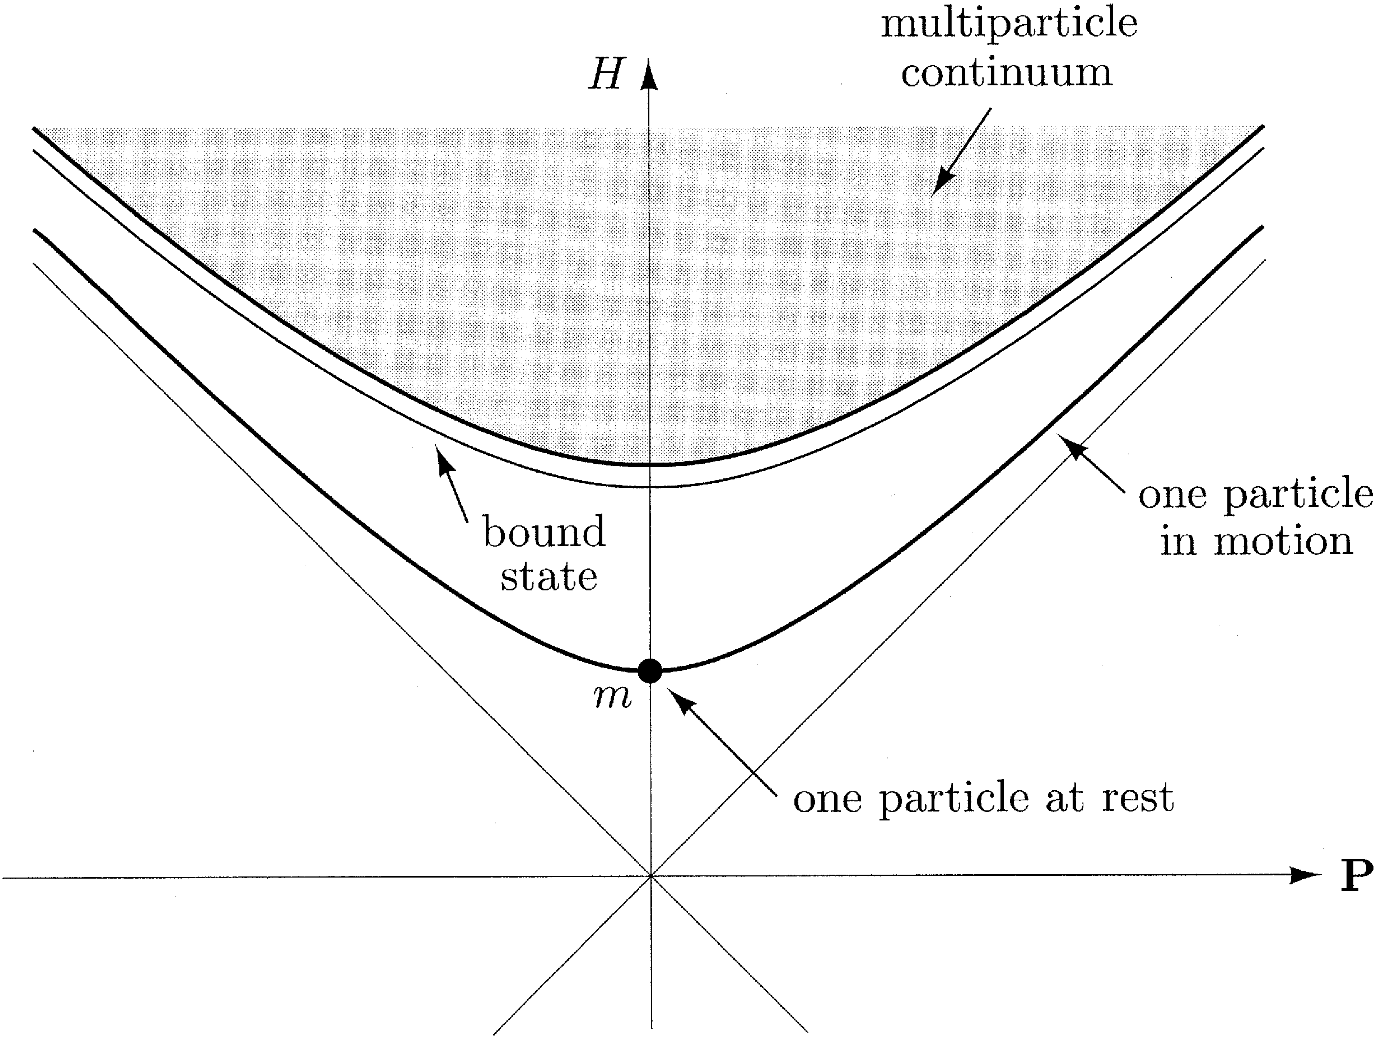
\includegraphics[width = 0.70 \textwidth]{images/mas-hyp.png}
  \caption{Hyperboloids in energy-momentum space formed by the eigenvalues of $ P^\mu = (H, \ve{P}) $.}
  \label{fig:mass-1}
\end{figure}

\begin{figure}[!ht]
  \centering
  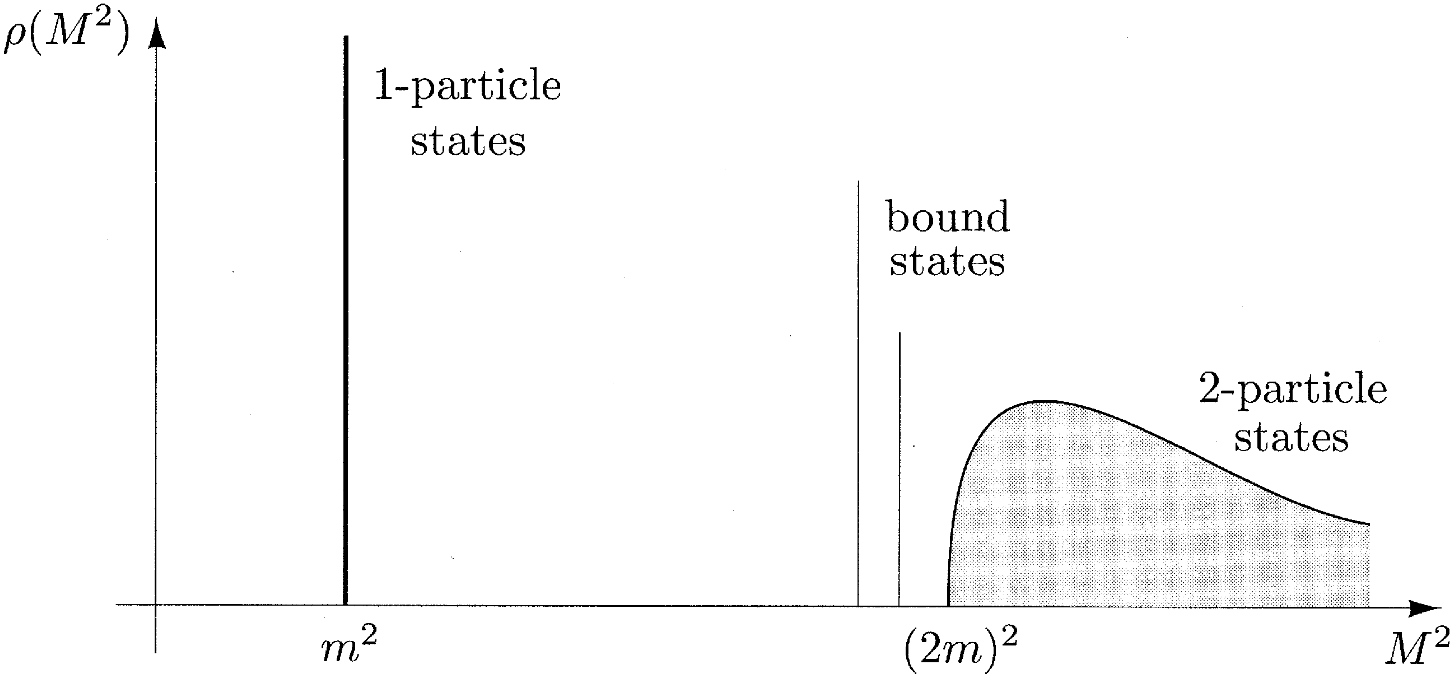
\includegraphics[width = 0.60 \textwidth]{images/spec-dens.png}
  \caption{Spectral density function for a typical interacting field theory.}
  \label{fig:mass-2}
\end{figure}

\begin{figure}[!ht]
  \centering
  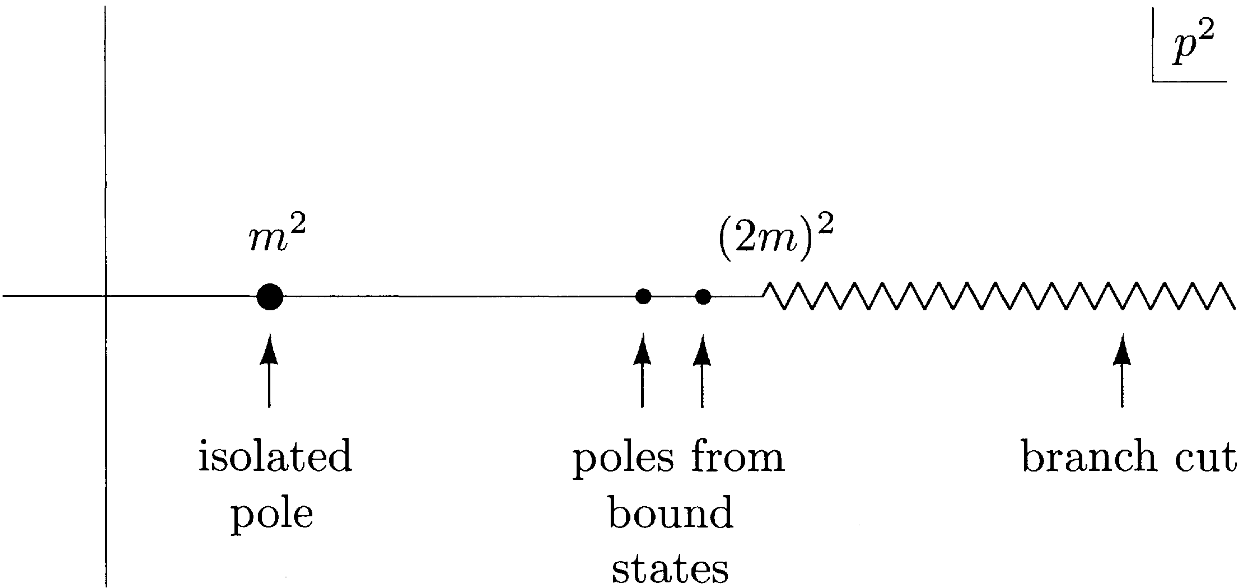
\includegraphics[width = 0.60 \textwidth]{images/poles.png}
  \caption{Analytic structure in the complex $ p^2 $-plane of $ \tilde{D}_\text{F}(p) $.}
  \label{fig:mass-3}
\end{figure}

As shown in Fig. \ref{fig:mass-2}, the one-particle states contribute to the spectral density with an isolated $ \delta $:
\begin{equation}
  \rho(M^2) = 2\pi \delta(M^2 - m^2) Z + (\text{terms with } M^2 \gtrsim (2m)^2)
\end{equation}
where $ Z $ is a number coming from the squared matrix element and it is called \bctxt{field-strength renormalization} (the same factor appearing in the LSZ reduction formula). Note that $ m $ is the physical mass of the particle, as opposed to the bare mass $ m_0 $ appearing in the Lagrangian. The Fourier transform of the $ 2 $-point Green function then is:
\begin{equation}
  \tilde{D}_\text{F}(p) = \frac{i Z}{p^2 - m^2 + i\epsilon} + \int_{\sim 4m^2}^\infty \frac{\dd M^2}{2\pi} \rho(M^2) \frac{i}{p^2 - M^2 + i\epsilon}
  \label{eq:corr-func-gen}
\end{equation}
The pole structure of $ \tilde{D}_\text{F}(p) $ is shown in Fig. \ref{fig:mass-3}: the first term gives an isolated simple pole in $ p^2 = m^2 $, while the second term contributes a branch cut beginning at $ p^2 = (2m)^2 $ (any two-particle bound states will appear as an additional $ \delta $ in $ \rho(M^2) $, i.e. additional an isolated pole below the branch cut). \eref{eq:corr-func-gen} is a direct generalization of \eref{eq:corr-func}: the former contains the field-strength renormalization $ Z = \abs{\braket{\lambda_0 | \phi(0) | 0}}^2 $, i.e. the probability for $ \phi(0) $ to create a given state from vacuum, while the latter has it implicitly, since in the free theory $ \abs{\braket{\ve{p} | \phi(0) | 0}}^2 = 1 $; moreover, \eref{eq:corr-func} is the amplitude of a single particle propagating from $ x $ to $ y $, as in the free theory $ \phi(0) $ can only create a single particle from vacuum, while \eref{eq:corr-func-gen} contains contributions from multiparticle intermediate states with a continuous mass spectrum.

\paragraph{Counterterms}

\eref{eq:corr-func-gen} has a single term which is singular at $ p^2 = m^2 $, and to eliminate the awkward residue $ Z $ it is possible to set:
\begin{equation}
  \phi \equiv \sqrt{Z} \phi_\text{r}
  \label{eq:phi-ren}
\end{equation}
This is the renormalized field (recall that it is equivalent to renormalize multiplicatively or additively).

\begin{proposition}{Renormalized $ \lambda \phi^4 $-theory}{}
  The renormalized Lagrangian of $ \lambda \phi^4 $-theory takes the form:
  \begin{equation}
    \lag = \frac{1}{2} \pa_\mu \phi_\text{r} \pa^\mu \phi_\text{r} - \frac{1}{2} m^2 \phi_\text{r}^2 - \frac{\lambda}{4!} \phi_\text{r}^4 + \frac{1}{2} \delta_Z \pa_\mu \phi_\text{r} \pa^\rho \phi_\text{r} - \frac{1}{2} \delta_m \phi_\text{r}^2 - \frac{\delta_\lambda}{4!} \phi_\text{r}^4
  \end{equation}
  with:
  \begin{equation}
    \delta_Z \equiv Z - 1
    \qquad \qquad
    \delta_m \equiv m_0^2 Z - m^2
    \qquad \qquad
    \delta_\lambda \equiv \lambda_0 Z^2 - \lambda
  \end{equation}
\end{proposition}

\begin{proofbox}
  \begin{proof}
    Inserting \eref{eq:phi-ren} into the Lagrangian of $ \lambda \phi^4 $-theory:
    \begin{equation*}
      \lag = \frac{1}{2} Z \pa_\mu \phi_\text{r} \pa^\mu \phi_\text{r} - \frac{1}{2} m_0^2 Z \phi_\text{r}^2 - \frac{\lambda_0}{4!} \phi_\text{r}^4
    \end{equation*}
    The isolation of counterterms is then trivial.
  \end{proof}
\end{proofbox}

This Lagrangian is composed of the standard $ \lambda \phi^4 $-theory Lagrangian, with renormalized field, mass and coupling constant, plus three counterterms: this is precisely the number of infinite constants appearing in diverging amplitudes of the theory. The Feynman rules for the renormalized theory are:
\begin{equation*}
  \begin{tikzpicture}[baseline=(r.base)]
    \begin{feynman}[inline=(r.base)]
      \vertex (a1) {};
      \vertex[right=4cm of a1] (a2) {};
      \vertex[below=4em of a1] (b1) {};
      \vertex[below=4em of a2] (b2) {};
      \vertex[below=2em of a1] (c1) {};
      \vertex[right=2cm of c1] (c2) {};

      \vertex[left = 2cm of c2] (d1) {};
      \vertex[right = 2cm of c2] (d2) {};

      \vertex[below=2.2em of a1] (r);

      \diagram* {
        (d1) -- [scalar, momentum = \(p\)] (d2),
      };
    \end{feynman}
  \end{tikzpicture}
  \quad = \quad \frac{i}{p^2 - m^2 + i\epsilon}
  \qquad
  \begin{tikzpicture}[baseline=(r.base)]
    \begin{feynman}[inline=(r.base)]
      \vertex (a1) {};
      \vertex[right=4cm of a1] (a2) {};
      \vertex[below=4em of a1] (b1) {};
      \vertex[below=4em of a2] (b2) {};
      \vertex[below=2em of a1] (c1) {};
      \vertex[right=2cm of c1, crossed dot] (c2) {};

      \vertex[left = 2cm of c2] (d1) {};
      \vertex[right = 2cm of c2] (d2) {};

      \vertex[below=2.2em of a1] (r);

      \diagram* {
        (d1) -- [scalar, momentum = \(p\)] (c2) -- [scalar] (d2),
      };
    \end{feynman}
  \end{tikzpicture}
  \quad = \quad i (p^2 \delta_Z - \delta_m)
\end{equation*}
\begin{equation*}
  \begin{tikzpicture}[baseline=(r.base)]
    \begin{feynman}[inline=(r.base)]
      \vertex (a1) {};
      \vertex[right=4cm of a1] (a2) {};
      \vertex[below=4em of a1] (b1) {};
      \vertex[below=4em of a2] (b2) {};
      \vertex[below=2em of a1] (c1) {};
      \vertex[right=2cm of c1, dot] (c2) {};

      \vertex[below=2.2em of a1] (r);

      \diagram* {
        (a1) -- [scalar] (c2),
        (b1) -- [scalar] (c2),
        (c2) -- [scalar] (a2),
        (c2) -- [scalar] (b2),
      };
    \end{feynman}
  \end{tikzpicture}
  \quad = \quad -i \lambda
  \qquad \qquad
  \begin{tikzpicture}[baseline=(r.base)]
    \begin{feynman}[inline=(r.base)]
      \vertex (a1) {};
      \vertex[right=4cm of a1] (a2) {};
      \vertex[below=4em of a1] (b1) {};
      \vertex[below=4em of a2] (b2) {};
      \vertex[below=2em of a1] (c1) {};
      \vertex[right=2cm of c1, crossed dot] (c2) {};

      \vertex[below=2.2em of a1] (r);

      \diagram* {
        (a1) -- [scalar] (c2),
        (b1) -- [scalar] (c2),
        (c2) -- [scalar] (a2),
        (c2) -- [scalar] (b2),
      };
    \end{feynman}
  \end{tikzpicture}
  \quad = \quad -i \delta_\lambda
\end{equation*}
To make the definition of the counterterms effective, the physical conditions which fix $ Z $, $ m $ and $ \lambda $ must be set, in order to set their value via comparison with experiments. The three \bctxt{renormalization conditions} are:
\begin{equation*}
  \begin{tikzpicture}[baseline=(r.base)]
    \begin{feynman}[inline=(r.base)]
      \vertex (a1) {};
      \vertex[right=4cm of a1] (a2) {};
      \vertex[below=4em of a1] (b1) {};
      \vertex[below=4em of a2] (b2) {};
      \vertex[below=2em of a1] (c1) {};
      \vertex[right=2cm of c1, blob] (c2) {};

      \vertex[left = 2cm of c2] (d1) {};
      \vertex[right = 2cm of c2] (d2) {};

      \vertex[below=2.2em of a1] (r);

      \diagram* {
        (d1) -- [scalar, momentum = \(p\)] (c2) -- [scalar] (d2),
      };
    \end{feynman}
  \end{tikzpicture}
  \quad = \quad \frac{i}{p^2 - m^2} + (\text{terms regular at } p^2 = m^2)
\end{equation*}
\begin{equation*}
  \begin{tikzpicture}[baseline=(r.base)]
    \begin{feynman}[inline=(r.base)]
      \vertex (a1) {};
      \vertex[right=4cm of a1] (a2) {};
      \vertex[below=4em of a1] (b1) {};
      \vertex[below=4em of a2] (b2) {};
      \vertex[below=2em of a1] (c1) {};
      \vertex[right=2cm of c1, blob] (c2) {};

      \vertex[below=2.2em of a1] (r);

      \diagram* {
        (a1) -- [scalar] (c2),
        (b1) -- [scalar] (c2),
        (c2) -- [scalar] (a2),
        (c2) -- [scalar] (b2),
      };
    \end{feynman}
  \end{tikzpicture}
  \quad = \quad -i \lambda
  \qquad \text{at} \qquad
  s = 4m^2 \,\,,\,\, t = u = 0
\end{equation*}
These physical conditions fix the pole and the residue of the $ 2 $-point Green function and the zero-momentum $ 2 \rightarrow 2 $ scattering amplitude: once loop integrals have been regularized, the $ \delta_Z $, $ \delta_m $ and $ \delta_\lambda $ are adjusted (renormalized) to satisfy the renormalization conditions and, after this adjustment, the amplitudes should be finite and independent of the regulator. This marks the successful renormalization of the theory\footnote{Note that in the $ \msb $ scheme the physical conditions are replaced by subtraction of poles: this means that the $ \msb $ mass $ m_{\msb} $ is not the pole of the $ 2 $-point Green function, hence it is not physically observable.}. \\
At $ \smo(\lambda) $ order only $ \delta_\lambda $ is non-trivial, as $ \delta_Z $ and $ \delta_m $ come into play only at $ \smo(\lambda)^2 $ with diagrams:
\begin{equation*}
  \begin{tikzpicture}[baseline = (r.base)]
    \begin{feynman}[inline = (r.base)]
      \vertex (x1) {};
      \vertex[below=3em of x1] (p1) {};
      \vertex[below=3em of p1] (x2) {};

      \vertex[right=3em of p1, dot] (v1) {};
      \vertex[right=5em of v1, dot] (v2) {};

      \vertex[right=3em of v2] (p2) {};
      \vertex[above=3em of p2] (x3) {};
      \vertex[below=3em of p2] (x4) {};

      \vertex[above=0.5em of v1] (r) {};

      \diagram* {
        (x1) -- [scalar] (v1),
        (x2) -- [scalar] (v1),
        (v2) -- [scalar] (x3),
        (v2) -- [scalar] (x4),

        (v1) -- [scalar, half left] (v2),
        (v2) -- [scalar, half left] (v1),
        (v1) -- [scalar] (v2),
      };
    \end{feynman}
  \end{tikzpicture}
  \quad + \quad
  \begin{tikzpicture}[baseline=(r.base)]
    \begin{feynman}[inline=(r.base)]
      \vertex (a1) {};
      \vertex[right=4cm of a1] (a2) {};
      \vertex[below=4em of a1] (b1) {};
      \vertex[below=4em of a2] (b2) {};
      \vertex[below=2em of a1] (c1) {};
      \vertex[right=2cm of c1, crossed dot] (c2) {};

      \vertex[left = 2cm of c2] (d1) {};
      \vertex[right = 2cm of c2] (d2) {};
      \vertex[above = 2cm of c2, empty dot] (d3) {};

      \vertex[above=1.1cm of c2] (r);

      \diagram* {
        (d1) -- [scalar] (c2) -- [scalar] (d2),
        (c2) -- [scalar, half left] (d3) -- [scalar, half left] (c2),
      };
    \end{feynman}
  \end{tikzpicture}
  \quad + \quad
  \begin{tikzpicture}[baseline=(r.base)]
    \begin{feynman}[inline=(r.base)]
      \vertex (a1) {};
      \vertex[right=4cm of a1] (a2) {};
      \vertex[below=4em of a1] (b1) {};
      \vertex[below=4em of a2] (b2) {};
      \vertex[below=2em of a1] (c1) {};
      \vertex[right=2cm of c1, crossed dot] (c2) {};

      \vertex[left = 2cm of c2] (d1) {};
      \vertex[right = 2cm of c2] (d2) {};

      \vertex[below=2.2em of a1] (r);

      \diagram* {
        (d1) -- [scalar] (c2) -- [scalar] (d2),
      };
    \end{feynman}
  \end{tikzpicture}
\end{equation*}
This means that:
\begin{equation}
  \delta_\lambda = 1 + \smo(\lambda)
  \qquad \qquad
  \delta_Z = 1 + \smo(\lambda^2)
  \qquad \qquad
  \delta_m = 1 + \smo(\lambda^2)
\end{equation}
agreeing with \secref{sssec:lag-count}. Tadpoles produces by the physical vertex (not the counterterm) should be considered too, but, as per \lref{lemma:tadpole-resumm}, they only contribute as a shift between $ m $ and $ m_0 $.












\bookmarksetupnext{level = -1}
\begin{appendices}
\pagestyle{append}

\chapter{Mathematical Reference}
\selectlanguage{english}

\section{Phase-space parametrization}
\label{sec:ph-sp-p}

In dimensional regularization with $ d = 4 - 2 \de $, we define the measure on the phase space of a parton $ i $ to be:
\begin{equation}
  [\dd p_i] \equiv \frac{\dd^{d-1} p_i}{(2\pi)^{d-1} 2E_i} \theta(\ema - E_i)
\end{equation}
Note that $ \ema $ is an upper bound on the energies of individual partons: it is an arbitrary parameter to be taken sufficiently large as to be greater or equal to the maximal energy that a final-state parton can reach.

This measure can be cast in a more useful form introducing a suitable parametrization of the phase space: in particular, given that $ \R^n-\{\ve{0}\} \cong \R^+ \times \mathbb{S}^{n-1} $, it is convenient to introduce hyperspherical coordinates on the $ \mathbb{S}^{d-2} $ component of the phase space. In general, the \bctxt{hyperspherical measure} on $ \mathbb{S}^n $ is recursively defined as:
\begin{equation}
  \dd \Omega_n = \sin^{n-1} \varphi \, \dd \varphi \, \dd \Omega_{n-1}
  \label{eq:hyp-rec}
\end{equation}
Using \eref{eq:hyp-rec} (with $ \sin \varphi \, \dd \varphi = \dd \cos \varphi $), we can express the measure $ \dd^{d-1} p_i $ as:
\begin{equation}
  \dd^{d-1} p_i = \abs{\ve{p}_i}^{d-2} \, \dd \abs{\ve{p}_i} \, \sin^{d-4} \varphi \, \dd \cos \varphi \, \dd \Omega_{d-2}
\end{equation}
As we are only interested in integrations on phase spaces of real unresolved partons, which can only be massless, we can use the on-shell condition $ p_i^2 = 0 $ to express $ \abs{\ve{p}_i} = E_i $, so that the phase-space measure becomes:
\begin{equation}
  [\dd p_i] = \theta(\ema - E_i) E_i^{d-3} \dd E_i \, \sin^{d-4} \varphi \, \dd \cos \varphi \, \frac{\dd \Omega_{d-2}}{2(2\pi)^{d-1}}
\end{equation}
with $ E_i \in \R^+ $ and $ \varphi \in [0,\pi] $.

\subsection{Multi-particle phase space}

When considering scattering processes, in general the final state is a multi-particle state, hence the measure on the final-state phase space must account for energy conservation too.

Given a $ 2 \rightarrow m $ scattering process with well-defined initial momenta $ p_\mathcal{A} $ and $ p_\mathcal{B} $, then the differential cross-section is (see Chapter 4 of \cite{Peskin-1995}):
\begin{equation}
  \dd\sigma = \frac{1}{2E_a 2E_b \abs{\ve{v}_a - \ve{v}_b}} \prod_{k = 1}^m \int \frac{\dd^3p_k}{(2\pi)^3 2E_k} \abs{\ampl(ab \rightarrow \mathcal{H})}^2 (2\pi)^4 \delta^{(4)}(p_a + p_b - \textstyle\sum_{i = 1}^m p_i)
  \label{eq:scatt-cr-sec}
\end{equation}
where $ \ampl(ab \rightarrow \mathcal{H}) $ is the amplitude of the scattering process and $ \ve{v}_k \equiv \frac{\ve{p}_k}{E_k} $ is the velocity of the $ k^\text{th} $ particle.

As we are only interested in massless initial-state partons, in the center-of-mass (CM) frame $ p_{a,b} = (E, \pm\ve{p}) $, hence it is trivial to see that the flux factor in \eref{eq:scatt-cr-sec} is just $ 2\hat{s} \defeq 2 (p_a + p_b)^2 $. The differential cross-section can then be rewritten as:
\begin{equation}
  \dd \sigma = \frac{1}{2\hat{s}} \int \lps_m \abs{\mat(ab \rightarrow \mathcal{H})}^2
\end{equation}
where the \bctxt{invariant $ m $-body phase space measure} is defined as:
\begin{equation}
  \lps_m \equiv \prod_{k = 1}^m [\dd p_k] (2\pi)^4 \delta^{(4)}(p_a + p_b - \sum_{i = 1}^m p_i)
\end{equation}

\section{Angular integrals}

\section{Partitions of unity}
\label{sec:unit-part}

To define a partition of unity such as \eref{eq:delta-part}, define $ \mathcal{H}^i \equiv \fsu{n}{m+1} - \{i\} $ and introduce the function:
\begin{equation}
  d^i \equiv \prod_{k \in \mathcal{H}^i} p_{k,\perp} \prod_{l < m \in \mathcal{H}^i} \rho_{lm}
\end{equation}
where $ p_{k,\perp} $ is the transverse momentum of the parton $ k $. Then, the partition is found as:
\begin{equation}
  \Delta^i \defeq \frac{d^i}{\sum_{j \in \fsu{n}{m+1}} d^j}
\end{equation}
These clearly provide a $ \fsu{n}{m+1} $-partition of unity. To prove its properties, note that:
\begin{equation*}
  \so_i d^j = \lim_{E_i \rightarrow 0} \prod_{k \in \mathcal{H}^i} p_{k,\perp} \prod_{l < m \in \mathcal{H}^i} \rho_{lm} =
  \begin{cases}
    0 & i \neq j \\
    d_j & i = j
  \end{cases}
\end{equation*}
Thus trivially $ \so_i \Delta^j = \delta_i^j $. The collinear limit is slightly more complex:
\begin{equation*}
  \co_{ij} d^k = \lim_{\rho_{ij} \rightarrow 0} \prod_{s \in \mathcal{H}^i} p_{s,\perp} \prod_{l < m \in \mathcal{H}^i} \rho_{lm} =
  \begin{cases}
    0 & i,j \neq k \\
    d^k & i = k \neq j
  \end{cases}
\end{equation*}
The latter case has two possibilities: either $ j \in \{a,b\} $ or $ j \in \mathcal{H}^i $. Then, clearly $ \co_{ia} d^i = \co_{ib} d^i = 1 $, while if $ j \in \mathcal{H}^i $:
\begin{equation*}
  \co_{ij} \Delta^i = \frac{d^i}{d^i + d^j} = \left[ 1 + \frac{d^j}{d^i} \right]^{-1}
\end{equation*}
With explicit calculation:
\begin{equation*}
  \frac{d^j}{d^i} = \frac{p_{i_\perp}}{p_{j,\perp}} \frac{\rho_{1,j} \dots \rho_{i-1,j} \rho_{i+1,j} \dots \rho_{j-1,j} \rho_{j,j+1} \dots \rho_{j,m+1}}{\rho_{1,i} \dots \rho_{i-1,i} \rho_{i,i+1} \dots \rho_{i,j-1} \rho_{i,j+1} \dots \rho_{i,m+1}} = \frac{p_{i,\perp}}{p_{j,\perp}} = \frac{E_i}{E_j}
\end{equation*}
where we have used the fact that $ \rho_{ik} \rightarrow \rho_{jk} \,\,\forall k \neq i,j $ as $ \rho_{ij} \rightarrow 0 $. This completes the proof.

To construct the angular partition of unity in \eref{eq:omega-part}, we set $ g_{kl} \equiv \rho_{kl}^{-1} $ and define the angular factors:
\begin{equation}
  \omega^{\ur i} \defeq \frac{g_{i\ur}}{\sum_{j \in \prt{n}{m}(\ur)} g_{j\ur}}
\end{equation}
These clearly provide a $ \prt{n}{m}(\ur) $-partition of unity. Moreover:
\begin{equation*}
  \co_{j\ur} \omega^{\ur i} = \lim_{\rho_{j\ur} \rightarrow 0} \frac{g_{i\ur}}{\sum_{k \in \prt{n}{m}(\ur)} g_{k\ur}} = \bigg[ \lim_{\rho_{j\ur} \rightarrow 0} \sum_{k \in \prt{n}{m}(\ur)} \frac{\rho_{i\ur}}{\rho_{k\ur}} \bigg]^{-1} =
  \begin{cases}
    1^{-1} & j = i \\
    \infty^{-1} & j \neq i
  \end{cases}
  = \delta^i_j
\end{equation*}
where we made an abuse of notation. This completes the proof.

\section{Quadratic Casimir operators of \texorpdfstring{$ \SUn{n_c} $}{SU(n)}}
\label{sec:cas-op}

To prove \eref{eq:cas-sun}, first consider the fundamental representation $ \mathtt{n} $ of $ \SUn{n_c} $.
Then, contracting \eref{eq:quad-cas} with $ \delta^{ab} $ (with $ a,b = 1,\dots, n^2 - 1 $, as they label the basis of $ \mathfrak{su}(n_c) $):
\begin{equation*}
  C_2(\mathtt{n}) n_c = \frac{1}{2} (n_c^2 - 1)
\end{equation*}
To compute the Casimir operator for the adjoint representation $ \mathtt{g} $, consider the decomposition of the direct product of two representations:
\begin{equation*}
  \mathtt{r}_1 \otimes \mathtt{r}_2 = \bigoplus_i \mathtt{r}_i
\end{equation*}
In this representation $ T^a_{\mathtt{r}_1 \otimes \mathtt{r}_2} = T^a_{\mathtt{r}_1} \otimes \id_{\mathtt{r}_2} + \id_{\mathtt{r}_1} \otimes T^a_{\mathtt{r}_2} $, and it acts on tensor objects $ \Xi_{pq} $ whose first index transforms according to $ \mathtt{r}_1 $ and the second index according to $ \mathtt{r}_2 $. Recalling that $ \tr{T^a} = 0 $:
\begin{equation*}
  \begin{split}
    \tr (T^a_{\mathtt{r}_1 \otimes \mathtt{r}_2})^2
    &= \tr ((T^a_{\mathtt{r}_1})^2 \otimes \id_{\mathtt{r}_2} + 2 T^a_{\mathtt{r}_1} \otimes T^a_{\mathtt{r}_2} + \id_{\mathtt{r}_1} \otimes (T^a_{\mathtt{r}_2})^2) \\
    &= \tr (C_2(\mathtt{r}_1) \id_{\mathtt{r}_1} \otimes \id_{\mathtt{r}_2}) + \tr (C_2(\mathtt{r}_2) \id_{\mathtt{r}_1} \otimes \id_{\mathtt{r}_2}) = (C_2(\mathtt{r}_1) + C_2(\mathtt{r}_2)) n_{\mathtt{r}_1} n_{\mathtt{r}_2}
  \end{split}
\end{equation*}
However, by the decomposition above:
\begin{equation*}
  \tr (T^a_{\mathtt{r}_1 \otimes \mathtt{r}_2})^2 = \sum_i C_2(\mathtt{r}_i) n_{\mathtt{r}_i}
\end{equation*}
Consider $ \mathtt{n} \otimes \mathtt{n}^* $, where $ \mathtt{n}^* $ is the complex conjugate of the fundamental representation (for complex representations, $ \mathtt{r} $ and $ \mathtt{r}^* $ are generally inequivalent representations): then $ \Xi_{pq} $ contains a term proportional to the invariant $ \delta_{pq} $, while the other $ n_c^2 - 1 $  independent components transform as a general $ n_c \times n_c $ traceless tensor, i.e. under the adjoint representation of $ \SUn{n_c} $ (as of \eeref{eq:sun-herm}{eq:sun-trace}), thus $ \mathtt{n} \otimes \mathtt{n}^* = \ve{1} \oplus \mathtt{g} $ and the above identity becomes:
\begin{equation*}
  (C_2(\ve{1}) + C_2(\mathtt{g})) (n_c^2 - 1) = (C_2(\mathtt{n}) + C_2(\mathtt{n}^*)) n_c^2
\end{equation*}
Using $ C_2(\ve{1}) = 0 $ (as all generators are trivially zero) and $ C_2(\mathtt{n}^*) = C_2(\mathtt{n}) $:
\begin{equation*}
  C_2(\mathtt{g}) (n_c^2 - 1) = \frac{n_c^2 - 1}{n_c} n_c^2
\end{equation*}
which completes the proof.












\chapter{Scattering Processes}
\selectlanguage{english}

\section{Cross-sections and \texorpdfstring{$ S $}{S}-matrix}

The cross-section generalizes the notion of geometric area of an object. Consider a flux of particles (particles per unit area per unit time):
\begin{equation*}
  j = \frac{\dd n}{\dd S \dd t}
\end{equation*}
Then, the number of incident particles diffused by a disk of section $ S $ in a time $ \Delta t $ is:
\begin{equation*}
  N = j S \Delta t
\end{equation*}
The (classical) \bctxt{cross-section} of the disk is then defined as:
\begin{equation}
  \sigma \defeq \frac{N}{j \Delta t}
\end{equation}
From a quantum point of view, $ N $ is the probability of the transition $ \ket{\text{i}} \rightarrow \ket{\text{f}} $ between the initial and final states, thus:
\begin{equation*}
  \dd \sigma = \frac{1}{j \Delta t} \abs{\braket{\text{f}(f) | \text{i}}}^2 \dd f
\end{equation*}
where $ f $ is some quantity which the final state depends on.

\subsection{Classical and quantum definition}

\subsection{Phase-space integration}

\begin{proposition}{Scattering cross-section}{}
  Given a $ 2 \rightarrow n $ scattering process with well-defined initial momenta $ p_\mathcal{A} $ and $ p_\mathcal{B} $, then the \bcprop{differential cross-section} is:
  \begin{equation}
    \dd\sigma = \frac{1}{2E_\mathcal{A} 2E_\mathcal{B} \abs{\ve{v}_\mathcal{A} - \ve{v}_\mathcal{B}}} \prod_{k = 1}^n \frac{\dd^3p_k}{(2\pi)^3 2E_k} \abs{\mathcal{M}(\mathcal{A} \mathcal{B} \rightarrow \{f\})}^2 (2\pi)^4 \delta^{(4)}(p_\mathcal{A} + p_\mathcal{B} - \textstyle\sum_{i = 1}^n p_i)
    \label{eq:scatt-cr-sec}
  \end{equation}
  where $ \mathcal{M}(\mathcal{A} \mathcal{B} \rightarrow \{f\}) $ is the matrix element of the scattering process and $ \ve{v}_k \equiv \frac{\ve{p}_k}{E_k} $ is the velocity of the $ k^\text{th} $ particle.
\end{proposition}

This cross-section is differential in $ 3n - 4 $ variables, as the momentum-conserving $ \delta^{(4)} $ allows to perform $ 4 $ integrations. The integration measure is defined as the \bctxt{invariant} $ n $\bctxt{-body phase space}:
\begin{equation}
  \int \dd \Pi_n \equiv \prod_{k = 1}^n \int \frac{\dd^3p_k}{(2\pi)^3 2E_k} (2\pi)^4 \delta^{(4)}(P - \textstyle\sum_{i = 1}^n p_i)
\end{equation}
with $ P $ the total initial 4-momentum.

\section{Feynman diagrams}


\clearpage
\end{appendices}

\bookmarksetupnext{level = -1}
\pagestyle{biblio}
\printbibliography[heading = bibintoc, title = {Bibliography}]

\end{document}
